\documentclass[
  paper=a4,
  fontsize=12pt,
  twoside,
  BCOR=8mm,
  DIV=calc,
  headings=small,
  parskip=half-,
  footnotes=multiple,
  numbers=noendperiod,
  ngerman,
]{scrbook}

\usepackage[ngerman]{babel}
\usepackage{fontspec}
\setmainfont{IBM Plex Serif}
\setsansfont{IBM Plex Sans}
\setmonofont{IBM Plex Mono}[Scale=MatchLowercase]
\usepackage[babel=true]{microtype}
\usepackage[autostyle]{csquotes}
\usepackage{xcolor}
\usepackage{graphicx}
\usepackage{longtable,booktabs,array,calc}
\usepackage{float}
\floatplacement{figure}{H}
\usepackage{scrlayer-scrpage}
\usepackage[noautomatic]{imakeidx}
\makeindex[intoc,columns=2,title=Stichwortverzeichnis]
\indexsetup{othercode=\small}
\newcommand{\indexgroup}[1]{\par\pagebreak[2]\bigskip{\sffamily\bfseries\color{akzent}#1}\par\nopagebreak\smallskip}
\usepackage[hidelinks,unicode]{hyperref}
\usepackage{xurl}

\recalctypearea
\makeatletter\renewcommand*\@pnumwidth{2.2em}\makeatother % dreistellige Seitenzahlen im Inhaltsverzeichnis
% Platz für zweistellige Kapitelnummern (10.1.1) im Inhaltsverzeichnis
\DeclareTOCStyleEntry[numwidth=2.8em]{tocline}{section}
\DeclareTOCStyleEntry[indent=4.3em,numwidth=3.8em]{tocline}{subsection}
\setlength{\emergencystretch}{3em}

% --- Farben (druckfreundlich, auch in Graustufen lesbar)
\definecolor{codebg}{gray}{0.95}
\definecolor{codekw}{HTML}{1F4E79}
\definecolor{codestr}{HTML}{7A3E00}
\definecolor{codecom}{gray}{0.40}
\definecolor{akzent}{HTML}{1F4E79}

% --- Überschriften und Kolumnentitel
\addtokomafont{disposition}{\color{akzent}}
\addtokomafont{chapterentry}{\color{black}}
\pagestyle{scrheadings}
\clearpairofpagestyles
\automark[section]{chapter}
\ohead{\headmark}
\ofoot*{\pagemark}
\setkomafont{pageheadfoot}{\normalfont\sffamily\footnotesize}

% --- Code (Hervorhebung durch pandoc/skylighting, Makros in build/highlight.tex)
\usepackage{fvextra}
\usepackage{color}
\usepackage{fancyvrb}
\newcommand{\VerbBar}{|}
\newcommand{\VERB}{\Verb[commandchars=\\\{\}]}
\DefineVerbatimEnvironment{Highlighting}{Verbatim}{commandchars=\\\{\}}
% Add ',fontsize=\small' for more characters per line
\usepackage{framed}
\definecolor{shadecolor}{RGB}{242,242,242}
\newenvironment{Shaded}{\begin{snugshade}}{\end{snugshade}}
\newcommand{\AlertTok}[1]{#1}
\newcommand{\AnnotationTok}[1]{\textcolor[rgb]{0.40,0.40,0.40}{\textit{#1}}}
\newcommand{\AttributeTok}[1]{#1}
\newcommand{\BaseNTok}[1]{\textcolor[rgb]{0.12,0.31,0.47}{#1}}
\newcommand{\BuiltInTok}[1]{\textcolor[rgb]{0.12,0.31,0.47}{#1}}
\newcommand{\CharTok}[1]{\textcolor[rgb]{0.48,0.24,0.00}{#1}}
\newcommand{\CommentTok}[1]{\textcolor[rgb]{0.40,0.40,0.40}{\textit{#1}}}
\newcommand{\CommentVarTok}[1]{\textcolor[rgb]{0.40,0.40,0.40}{\textit{#1}}}
\newcommand{\ConstantTok}[1]{\textcolor[rgb]{0.12,0.31,0.47}{#1}}
\newcommand{\ControlFlowTok}[1]{\textcolor[rgb]{0.12,0.31,0.47}{\textbf{#1}}}
\newcommand{\DataTypeTok}[1]{#1}
\newcommand{\DecValTok}[1]{\textcolor[rgb]{0.12,0.31,0.47}{#1}}
\newcommand{\DocumentationTok}[1]{\textcolor[rgb]{0.40,0.40,0.40}{\textit{#1}}}
\newcommand{\ErrorTok}[1]{#1}
\newcommand{\ExtensionTok}[1]{#1}
\newcommand{\FloatTok}[1]{\textcolor[rgb]{0.12,0.31,0.47}{#1}}
\newcommand{\FunctionTok}[1]{\textcolor[rgb]{0.12,0.31,0.47}{#1}}
\newcommand{\ImportTok}[1]{#1}
\newcommand{\InformationTok}[1]{#1}
\newcommand{\KeywordTok}[1]{\textcolor[rgb]{0.12,0.31,0.47}{\textbf{#1}}}
\newcommand{\NormalTok}[1]{#1}
\newcommand{\OperatorTok}[1]{#1}
\newcommand{\OtherTok}[1]{#1}
\newcommand{\PreprocessorTok}[1]{#1}
\newcommand{\RegionMarkerTok}[1]{#1}
\newcommand{\SpecialCharTok}[1]{#1}
\newcommand{\SpecialStringTok}[1]{\textcolor[rgb]{0.48,0.24,0.00}{#1}}
\newcommand{\StringTok}[1]{\textcolor[rgb]{0.48,0.24,0.00}{#1}}
\newcommand{\VariableTok}[1]{#1}
\newcommand{\VerbatimStringTok}[1]{\textcolor[rgb]{0.48,0.24,0.00}{#1}}
\newcommand{\WarningTok}[1]{#1}

\fvset{fontsize=\small,breaklines=true,listparameters={\setlength{\topsep}{0pt}\setlength{\partopsep}{0pt}}}
\setlength{\FrameSep}{0.6em}
% Kasten mit Innenabstand, aber innerhalb des Satzspiegels
\renewenvironment{Shaded}{%
  \def\FrameCommand{\fboxsep=\FrameSep\colorbox{shadecolor}}%
  \MakeFramed{\advance\hsize-\width\FrameRestore}%
  \parskip=0pt\topsep=0pt\partopsep=0pt}%
  {\endMakeFramed}

% Hinweiskasten (im Original: notice.html)
\newenvironment{hinweis}[1]{%
  \def\FrameCommand{{\color{akzent}\vrule width 2.5pt}\hspace{0.8em}}%
  \MakeFramed{\advance\hsize-\width\FrameRestore}%
  \noindent{\sffamily\bfseries\color{akzent}#1}\par\nobreak}%
  {\endMakeFramed}

% pandoc-Hilfsmakros
\providecommand{\pandocbounded}[1]{#1}
\setkomafont{caption}{\small\sffamily}
\providecommand{\tightlist}{\setlength{\itemsep}{0pt}\setlength{\parskip}{0pt}}
\newcommand{\passthrough}[1]{#1}

\hypersetup{
  pdftitle={Luanti-Modding-Buch},
  pdfauthor={rubenwardy},
  pdflang={de-DE},
}

\begin{document}

% ---------------------------------------------------------------- Titelei
\frontmatter

\extratitle{\centering\vspace*{0.3\textheight}
  {\usekomafont{title}\Huge Luanti-Modding-Buch}}
\titlehead{}
\title{Luanti-Modding-Buch}
\subtitle{Eigene Mods und Spiele für Luanti entwickeln}
\author{rubenwardy}
\publishers{%
  \normalsize
  Lektorat: Shara}
\date{}

\uppertitleback{}
\lowertitleback{\small
  \textbf{Luanti-Modding-Buch}\\
  Originaltitel: \emph{Luanti Modding Book}\\[1ex]
  Text: rubenwardy, \url{https://rubenwardy.com}\\[1ex]
  Quelle: \url{https://gitlab.com/rubenwardy/minetest_modding_book}\\
  Stand der Quelle: Commit b3904f8 (23.\,10.\,2026)\\[1ex]
  Dieses Werk ist lizenziert unter der Creative-Commons-Lizenz
  \enquote{Namensnennung -- Weitergabe unter gleichen Bedingungen 4.0
  International} (CC BY-SA 4.0):\\
  \url{https://creativecommons.org/licenses/by-sa/4.0/deed.de}\\[1ex]
  Die deutsche Übersetzung wurde für diese Ausgabe aus dem englischen
  Original erstellt. Die Bezeichnung \enquote{Minetest} wurde
  durchgehend auf \enquote{Luanti}, der API-Namensraum \texttt{minetest} auf
  \texttt{core} aktualisiert.\\[1ex]
  Gesetzt aus der IBM Plex mit \LaTeX{} und KOMA-Script.}

\maketitle

\tableofcontents

\addchap{Einleitung}
\label{ch:index}

Luanti verwendet Lua-Skripte, um Modding zu ermöglichen. Dieses Buch
soll dir, beginnend mit den Grundlagen, beibringen, wie du deine eigenen
Mods erstellst. Jedes Kapitel konzentriert sich auf einen bestimmten
Teil der API und bringt dich schnell dahin, eigene Mods zu schreiben.

Das Buch ist auch online lesbar\footnote{\url{https://rubenwardy.com/minetest_modding_book/de/}}
und als HTML herunterladbar\footnote{\url{https://gitlab.com/rubenwardy/minetest_modding_book/-/releases}}.

\section*{Feedback und Beiträge}\label{feedback-und-beitruxe4ge}
\addcontentsline{toc}{section}{Feedback und Beiträge}

Hast du einen Fehler bemerkt oder möchtest du Feedback geben? Dann teile
es bitte mit:

\begin{itemize}
\tightlist
\item
  Erstelle ein Issue auf GitLab\footnote{\url{https://gitlab.com/rubenwardy/minetest_modding_book/-/issues}}.
\item
  Schreib im Forenthema\footnote{\url{https://forum.luanti.org/viewtopic.php?f=14&t=10729}}
  oder im deutschen Forenthema\footnote{\url{https://forum.luanti.org/viewtopic.php?t=26723}}.
\item
  Nimm Kontakt mit dem Autor auf\footnote{\url{https://rubenwardy.com/contact/}}.
\item
  Lust mitzumachen? Lies die README\footnote{\url{https://gitlab.com/rubenwardy/minetest_modding_book/-/blob/master/README.md}}.
\end{itemize}


% ---------------------------------------------------------------- Hauptteil
\mainmatter

\part{Grundlagen}
\chapter{Erste Schritte}
\label{ch:basics/getting-started}

Den grundlegenden Aufbau eines Mod-Verzeichnisses zu verstehen, ist beim
Erstellen von Mods unerlässlich. In diesem Kapitel erfährst du, wie
Modding in Luanti funktioniert, und erstellst deinen ersten Mod.

\section{Was sind Spiele und Mods?}\label{was-sind-spiele-und-mods}

Die Stärke von Luanti liegt darin, dass sich Spiele einfach entwickeln
lassen, ohne eigene Voxel-Grafik, Voxel-Algorithmen oder ausgefeilten
Netzwerkcode schreiben zu müssen.

In Luanti ist ein Spiel eine Sammlung von Modulen, die zusammenarbeiten,
um den Inhalt und das Verhalten des Spiels bereitzustellen. Ein Modul,
allgemein als Mod bezeichnet, ist eine Sammlung von Skripten und
Ressourcen. Es ist möglich, ein Spiel mit nur einem Mod zu erstellen,
aber das wird selten gemacht, weil sich dann Teile des Spiels nicht mehr
so einfach unabhängig voneinander anpassen oder ersetzen lassen.

Ebenso ist es möglich, Mods außerhalb eines Spiels zu verbreiten. Dann
sind sie ebenfalls \emph{Mods}, aber im traditionelleren Sinn:
\emph{Modifikationen}. Diese Mods verändern oder erweitern die
Eigenschaften eines Spiels.

Sowohl die Mods, die in einem Spiel enthalten sind, als auch Mods von
Dritten nutzen dieselbe API (Programmierschnittstelle).

Dieses Buch behandelt die wichtigsten Teile der Luanti-API und richtet
sich gleichermaßen an Spieleentwickler und Modder.

\section{Wo werden die Mods
gespeichert?}\label{wo-werden-die-mods-gespeichert}

Jeder Mod hat sein eigenes Verzeichnis, in dem sich seine
Lua-Quelltexte, Texturen,\index{textur@Textur} Modelle und Tondateien
befinden. Luanti sucht an verschiedenen Orten nach Mods. Diese Orte
werden allgemein \emph{Mod-Ladepfade} genannt.

Für eine bestimmte Welt werden drei Mod-Speicherorte geprüft, und zwar
in dieser Reihenfolge:

\begin{enumerate}
\def\labelenumi{\arabic{enumi}.}
\tightlist
\item
  Spiel-Mods. Das sind die Mods des Spiels, in dem die Welt läuft.\\
  Z.~B.:
  \texttt{minetest/\allowbreak{}games/\allowbreak{}minetest\_\allowbreak{}game/\allowbreak{}mods/\allowbreak{}}
  oder\\
  \texttt{/\allowbreak{}usr/\allowbreak{}share/\allowbreak{}minetest/\allowbreak{}games/\allowbreak{}minetest/\allowbreak{}}
\item
  Globale Mods. Der Ort, an dem Mods fast immer installiert werden. Im
  Zweifelsfall legst du Mods hier ab.\\
  Z.~B.: \texttt{minetest/\allowbreak{}mods/\allowbreak{}}
\item
  Welt-Mods. Der Ort für Mods, die zu einer bestimmten Welt gehören.\\
  Z.~B.:
  \texttt{minetest/\allowbreak{}worlds/\allowbreak{}world/\allowbreak{}worldmods/\allowbreak{}}
\end{enumerate}

\texttt{minetest} ist das
Benutzerdatenverzeichnis.\index{benutzerdatenverzeichnis@Benutzerdatenverzeichnis}
Seinen Ort findest du, indem du Luanti öffnest und in der Registerkarte
„Über`` auf „Benutzerdatenverzeichnis öffnen`` klickst. Wurde Luanti
über Flathub installiert, passiert bei diesem Klick unter Umständen
nichts. Das Verzeichnis liegt dann normalerweise unter
\texttt{\textasciitilde{}/.\allowbreak{}var/\allowbreak{}app/\allowbreak{}org.\allowbreak{}luanti.\allowbreak{}luanti/.\allowbreak{}minetest/\allowbreak{}}.

Beim Laden prüft Luanti die oben genannten Orte der Reihe nach. Stößt es
auf einen Mod mit demselben Namen wie ein zuvor gefundener, wird der
spätere anstelle des früheren geladen. Du kannst also Spiel-Mods
überschreiben, indem du einen gleichnamigen Mod in das globale
Mod-Verzeichnis legst.

\section{Deinen ersten Mod erstellen}\label{deinen-ersten-mod-erstellen}

\subsection{Mod-Verzeichnis}\label{mod-verzeichnis}

Geh in das globale Mod-Verzeichnis (Über \textgreater{}
Benutzerdatenverzeichnis öffnen \textgreater{} mods) und lege einen
neuen Ordner namens \texttt{mymod} an. \texttt{mymod} ist der Name des
Mods.

Jeder Mod sollte einen eindeutigen \emph{Mod-Namen} haben, eine
technische Kennung (ID), über die auf den Mod verwiesen wird. Mod-Namen
dürfen Buchstaben, Ziffern und Unterstriche enthalten. Ein guter Name
beschreibt, was der Mod tut. Das Verzeichnis mit den Bestandteilen eines
Mods muss genauso heißen wie der Mod. Ob ein Mod-Name noch frei ist,
findest du mit einer Suche auf \url{https://content.luanti.org} heraus.

\begin{Shaded}
\begin{Highlighting}[]
\NormalTok{mymod}
\NormalTok{├── textures}
\NormalTok{│   └── mymod\_node.png}
\NormalTok{├── init.lua}
\NormalTok{└── mod.conf}
\end{Highlighting}
\end{Shaded}

Ein Mod benötigt nur eine
\texttt{init.\allowbreak{}lua}\index{init.lua@\texttt{init.\allowbreak{}lua}}.
Eine
\texttt{mod.\allowbreak{}conf}\index{mod.conf@\texttt{mod.\allowbreak{}conf}}
wird jedoch empfohlen, und je nach Funktionsumfang können weitere
Bestandteile nötig sein.

\subsection{mod.conf}\label{mod.conf}

Lege eine Datei \texttt{mod.\allowbreak{}conf} mit folgendem Inhalt an:

\begin{Shaded}
\begin{Highlighting}[]
\NormalTok{name = mymod}
\NormalTok{description = Fügt foo, bar und bo hinzu.}
\NormalTok{depends = default}
\end{Highlighting}
\end{Shaded}

Diese Datei enthält die Metadaten\index{metadaten@Metadaten} des Mods,
darunter seinen Namen, seine Beschreibung und weitere Angaben.

\subsection{init.lua}\label{init.lua}

Lege eine Datei \texttt{init.\allowbreak{}lua} mit folgendem Inhalt an:

\begin{Shaded}
\begin{Highlighting}[]
\FunctionTok{print}\OperatorTok{(}\StringTok{"Diese Datei wird beim Laden ausgeführt!"}\OperatorTok{)}

\VariableTok{core}\OperatorTok{.}\NormalTok{register\_node}\OperatorTok{(}\StringTok{"mymod:node"}\OperatorTok{,} \OperatorTok{\{}
    \VariableTok{description} \OperatorTok{=} \StringTok{"Das ist ein Node"}\OperatorTok{,}
    \VariableTok{tiles} \OperatorTok{=} \OperatorTok{\{} \StringTok{"mymod\_node.png"} \OperatorTok{\},}
    \VariableTok{groups} \OperatorTok{=} \OperatorTok{\{} \VariableTok{cracky} \OperatorTok{=} \DecValTok{1} \OperatorTok{\},}
\OperatorTok{\})}

\VariableTok{core}\OperatorTok{.}\NormalTok{register\_craft}\OperatorTok{(\{}
    \FunctionTok{type} \OperatorTok{=} \StringTok{"shapeless"}\OperatorTok{,}
    \VariableTok{output} \OperatorTok{=} \StringTok{"mymod:node 3"}\OperatorTok{,}
    \VariableTok{recipe} \OperatorTok{=} \OperatorTok{\{} \StringTok{"default:dirt"}\OperatorTok{,} \StringTok{"default:stone"} \OperatorTok{\},}
\OperatorTok{\})}
\end{Highlighting}
\end{Shaded}

Die \texttt{init.\allowbreak{}lua} ist der Einstiegspunkt eines Mods und
wird ausgeführt, wenn der Mod geladen wird.

\subsection{Zusammenfassung}\label{zusammenfassung}

Dieser Mod heißt „mymod``. Er besteht aus zwei Textdateien:
\texttt{init.\allowbreak{}lua} und \texttt{mod.\allowbreak{}conf}. Das
Skript gibt eine Nachricht aus und registriert dann einen Node und ein
Handwerksrezept -- beides wird später erklärt. Es gibt eine einzige
Abhängigkeit, den default-Mod\footnote{\url{https://content.luanti.org/metapackages/default/}},
der normalerweise in Minetest Game enthalten ist. Außerdem liegt in
\texttt{textures/\allowbreak{}} eine Textur für den Node.

\section{Abhängigkeiten}\label{abhuxe4ngigkeiten}

Eine Abhängigkeit besteht, wenn ein Mod einen anderen Mod benötigt, der
vor ihm geladen werden muss. Ein Mod kann darauf angewiesen sein, dass
Code, Gegenstände oder andere Ressourcen eines anderen Mods verfügbar
sind.

Es gibt zwei Arten von Abhängigkeiten: feste und optionale. Bei beiden
wird der andere Mod zuerst geladen. Ist der Mod, von dem abgehangen
wird, nicht verfügbar, führt eine feste Abhängigkeit dazu, dass der
eigene Mod nicht geladen wird, während eine optionale Abhängigkeit
höchstens dazu führt, dass weniger Funktionen zur Verfügung stehen.

Eine optionale Abhängigkeit ist nützlich, wenn du einen anderen Mod
optional unterstützen möchtest; so lassen sich zusätzliche Inhalte
aktivieren, wenn der Benutzer beide Mods gleichzeitig verwendet.

Abhängigkeiten werden in der \texttt{mod.\allowbreak{}conf} als
kommagetrennte Liste angegeben:

\begin{Shaded}
\begin{Highlighting}[]
\NormalTok{depends = modeins, modzwei}
\NormalTok{optional\_depends = moddrei}
\end{Highlighting}
\end{Shaded}

\section{Mod-Pakete}\label{mod-pakete}

Mods lassen sich zu Mod-Paketen\index{mod-paket@Mod-Paket} (Modpacks)
zusammenfassen, sodass mehrere Mods gemeinsam verpackt und verschoben
werden können. Das ist nützlich, wenn du einem Spieler mehrere Mods
bereitstellen möchtest, ohne dass er jeden einzeln herunterladen muss.

\begin{Shaded}
\begin{Highlighting}[]
\NormalTok{modpack1}
\NormalTok{├── modpack.conf (erforderlich, kennzeichnet Mod{-}Paket)}
\NormalTok{├── mod1}
\NormalTok{│   └── ... Mod{-}Dateien}
\NormalTok{└── mymod (optional)}
\NormalTok{    └── ... Mod{-}Dateien}
\end{Highlighting}
\end{Shaded}

Beachte, dass ein Mod-Paket kein \emph{Spiel} ist. Spiele haben eine
eigene Verzeichnisstruktur, die im Kapitel „Spiele`` erklärt wird.

\chapter{Lua-Skripting}
\label{ch:basics/lua}

In diesem Kapitel lernst du die Skripterstellung in Lua kennen, die
Werkzeuge, die dir dabei helfen, und einige Techniken, die du nützlich
finden wirst.

\section{Programmierung}\label{programmierung}

Beim Programmieren geht es darum, ein Problem -- etwa das Sortieren
einer Liste -- in Schritte zu zerlegen, die ein Computer verstehen kann.
Den logischen Prozess des Programmierens zu vermitteln, würde den Rahmen
dieses Buches sprengen; die folgenden Angebote sind dafür aber sehr
hilfreich:

\begin{itemize}
\tightlist
\item
  Codecademy\footnote{\url{http://www.codecademy.com/}} (englisch) ist
  eine der besten Quellen, um Programmieren zu lernen. Sie bietet
  interaktive Lerneinheiten.
\item
  Scratch\footnote{\url{https://scratch.mit.edu}} eignet sich gut, um
  bei den absoluten Grundlagen anzufangen und die
  Problemlösungstechniken zu erlernen, die man zum Programmieren
  braucht. Besonders gut geeignet für Kinder und Jugendliche.
\item
  The Morpheus\footnote{\url{https://www.youtube.com/@TheMorpheusTutorials}}
  ist ein guter YouTube-Kanal, um programmieren zu lernen.
\end{itemize}

\subsection{Programmieren in Lua}\label{programmieren-in-lua}

Auch Lua selbst zu lehren, würde über dieses Buch hinausgehen. Das Buch
Programming in Lua (PiL)\footnote{\url{https://www.lua.org/pil/contents.html}}
(englisch) ist jedoch eine ausgezeichnete Einführung in die
Programmierung mit Lua.

\section{Code-Editoren}\label{code-editoren}

Zum Schreiben von Lua-Skripten genügt ein Code-Editor mit
Syntaxhervorhebung. Dabei werden Wörter und Zeichen je nach Bedeutung
unterschiedlich eingefärbt. So fallen Fehler und Ungereimtheiten leicht
auf.

Zum Beispiel:

\begin{Shaded}
\begin{Highlighting}[]
\KeywordTok{function} \VariableTok{ctf}\OperatorTok{.}\NormalTok{post}\OperatorTok{(}\VariableTok{team}\OperatorTok{,} \VariableTok{msg}\OperatorTok{)}
    \ControlFlowTok{if} \KeywordTok{not} \VariableTok{ctf}\OperatorTok{.}\NormalTok{team}\OperatorTok{(}\VariableTok{team}\OperatorTok{)} \ControlFlowTok{then}
        \ControlFlowTok{return} \KeywordTok{false}
    \ControlFlowTok{end}
    \ControlFlowTok{if} \KeywordTok{not} \VariableTok{ctf}\OperatorTok{.}\NormalTok{team}\OperatorTok{(}\VariableTok{team}\OperatorTok{).}\VariableTok{log} \ControlFlowTok{then}
        \VariableTok{ctf}\OperatorTok{.}\NormalTok{team}\OperatorTok{(}\VariableTok{team}\OperatorTok{).}\VariableTok{log} \OperatorTok{=} \OperatorTok{\{\}}
    \ControlFlowTok{end}

    \FunctionTok{table.insert}\OperatorTok{(}\VariableTok{ctf}\OperatorTok{.}\NormalTok{team}\OperatorTok{(}\VariableTok{team}\OperatorTok{).}\VariableTok{log}\OperatorTok{,} \DecValTok{1}\OperatorTok{,} \VariableTok{msg}\OperatorTok{)}
    \VariableTok{ctf}\OperatorTok{.}\NormalTok{save}\OperatorTok{()}

    \ControlFlowTok{return} \KeywordTok{true}
\KeywordTok{end}
\end{Highlighting}
\end{Shaded}

In diesem Beispiel sind die Schlüsselwörter hervorgehoben, darunter
\texttt{if}, \texttt{then}, \texttt{end} und \texttt{return}.
Funktionen, die Lua standardmäßig mitbringt, etwa
\texttt{table.\allowbreak{}insert}, werden ebenfalls hervorgehoben.

Für den Einstieg empfehlen sich diese Editoren:

\begin{itemize}
\tightlist
\item
  VSCode\footnote{\url{https://code.visualstudio.com/}} bzw. die
  quelloffene Variante VSCodium\footnote{\url{https://vscodium.com/}}:
  verbreitet und für alle Betriebssysteme erhältlich. Installiere dazu
  die Erweiterung Lua\footnote{\url{https://marketplace.visualstudio.com/items?itemName=sumneko.lua}}
  (Lua Language Server). Sie vervollständigt Code automatisch, zeigt
  Fehler schon beim Tippen an und springt auf Wunsch zur Definition
  einer Funktion. Ergänzend gibt es Erweiterungen speziell für
  Luanti\footnote{\url{https://marketplace.visualstudio.com/items?itemName=GreenXenith.minetest-tools}}.
\item
  Notepad++\footnote{\url{http://notepad-plus-plus.org/}} (englisch):
  schlicht, nur für Windows.
\end{itemize}

Es gibt auch andere geeignete Editoren.

\section{Lokaler und globaler
Gültigkeitsbereich}\label{lokaler-und-globaler-guxfcltigkeitsbereich}

Ob eine Variable lokal oder global ist, bestimmt, von wo aus sie gelesen
und beschrieben werden kann. Auf globale Variablen kann von überall in
der Skriptdatei und auch von jedem anderen Mod aus zugegriffen werden:

\begin{Shaded}
\begin{Highlighting}[]
\KeywordTok{function}\NormalTok{ one}\OperatorTok{()}
    \VariableTok{foo} \OperatorTok{=} \StringTok{"bar"}
\KeywordTok{end}

\KeywordTok{function}\NormalTok{ two}\OperatorTok{()}
    \FunctionTok{print}\OperatorTok{(}\FunctionTok{dump}\OperatorTok{(}\VariableTok{foo}\OperatorTok{))} \CommentTok{{-}{-} Ausgabe: "bar"}
\KeywordTok{end}

\NormalTok{one}\OperatorTok{()}
\NormalTok{two}\OperatorTok{()}
\end{Highlighting}
\end{Shaded}

Auf eine lokale Variable kann dagegen nur dort zugegriffen werden, wo
sie definiert ist. In Lua sind Variablen standardmäßig global; du musst
daher ausdrücklich das Schlüsselwort \texttt{local} verwenden:

\begin{Shaded}
\begin{Highlighting}[]
\CommentTok{{-}{-} Innerhalb dieser Skriptdatei zugänglich}
\KeywordTok{local} \VariableTok{one} \OperatorTok{=} \DecValTok{1}

\KeywordTok{function}\NormalTok{ myfunc}\OperatorTok{()}
    \CommentTok{{-}{-} Innerhalb dieser Funktion zugänglich}
    \KeywordTok{local} \VariableTok{two} \OperatorTok{=} \VariableTok{one} \OperatorTok{+} \VariableTok{one}

    \ControlFlowTok{if} \VariableTok{two} \OperatorTok{==} \VariableTok{one} \ControlFlowTok{then}
        \CommentTok{{-}{-} Innerhalb dieser if{-}Anweisung zugänglich}
        \KeywordTok{local} \VariableTok{three} \OperatorTok{=} \VariableTok{one} \OperatorTok{+} \VariableTok{two}
    \ControlFlowTok{end}
\KeywordTok{end}
\end{Highlighting}
\end{Shaded}

\subsection{Möglichst lokale Variablen
verwenden}\label{muxf6glichst-lokale-variablen-verwenden}

Wann immer möglich, sollten lokale Variablen verwendet werden. Ein Mod
sollte höchstens eine globale Variable anlegen, und zwar mit demselben
Namen wie der Mod. Weitere globale Variablen sind unsauberer
Programmierstil, und Luanti warnt davor:

\begin{Shaded}
\begin{Highlighting}[]
\NormalTok{Assignment to undeclared global \textquotesingle{}foo\textquotesingle{} inside function}
\NormalTok{at init.lua:2}
\end{Highlighting}
\end{Shaded}

Sinngemäß: Zuweisung an die nicht deklarierte globale Variable
\texttt{foo} innerhalb einer Funktion in
\texttt{init.\allowbreak{}lua}\index{init.lua@\texttt{init.\allowbreak{}lua}},
Zeile 2.

Um das zu beheben, verwende \texttt{local}:

\begin{Shaded}
\begin{Highlighting}[]
\KeywordTok{function}\NormalTok{ one}\OperatorTok{()}
    \KeywordTok{local} \VariableTok{foo} \OperatorTok{=} \StringTok{"bar"}
\KeywordTok{end}

\KeywordTok{function}\NormalTok{ two}\OperatorTok{()}
    \FunctionTok{print}\OperatorTok{(}\FunctionTok{dump}\OperatorTok{(}\VariableTok{foo}\OperatorTok{))} \CommentTok{{-}{-} Ausgabe: nil}
\KeywordTok{end}

\NormalTok{one}\OperatorTok{()}
\NormalTok{two}\OperatorTok{()}
\end{Highlighting}
\end{Shaded}

Denk daran, dass \texttt{nil} \textbf{nicht initialisiert} bedeutet: Der
Variablen wurde noch kein Wert zugewiesen, sie existiert nicht, oder ihr
Wert wurde entfernt (also auf \texttt{nil} gesetzt).

Funktionen sind Variablen eines besonderen Typs, sollten aber ebenfalls
lokal sein, weil andere Mods Funktionen mit demselben Namen haben
könnten.

\begin{Shaded}
\begin{Highlighting}[]
\KeywordTok{local} \KeywordTok{function}\NormalTok{ foo}\OperatorTok{(}\VariableTok{bar}\OperatorTok{)}
    \ControlFlowTok{return} \VariableTok{bar} \OperatorTok{*} \DecValTok{2}
\KeywordTok{end}
\end{Highlighting}
\end{Shaded}

Damit andere Mods deine Funktionen aufrufen können, lege eine Tabelle
mit demselben Namen wie der Mod an und füge deine Funktionen dort ein.
Diese Tabelle wird oft als API-Tabelle oder
Namensraum\index{namensraum@Namensraum} (\emph{namespace}) bezeichnet.

\begin{Shaded}
\begin{Highlighting}[]
\VariableTok{mymod} \OperatorTok{=} \OperatorTok{\{\}}

\KeywordTok{function} \VariableTok{mymod}\OperatorTok{.}\NormalTok{foo}\OperatorTok{(}\VariableTok{bar}\OperatorTok{)}
    \ControlFlowTok{return} \StringTok{"foo"} \OperatorTok{..} \VariableTok{bar}
\KeywordTok{end}

\CommentTok{{-}{-} In einem anderen Mod oder Skript:}
\VariableTok{mymod}\OperatorTok{.}\NormalTok{foo}\OperatorTok{(}\StringTok{"foobar"}\OperatorTok{)}
\end{Highlighting}
\end{Shaded}

Die Schreibweise \texttt{function mymod.\allowbreak{}foo()} ist
gleichbedeutend mit \texttt{mymod.\allowbreak{}foo = function()}, nur
etwas lesbarer.

\section{Andere Lua-Skripte
einbinden}\label{andere-lua-skripte-einbinden}

Andere Lua-Skripte bindet man in einen Mod am besten mit
\emph{dofile\index{dofile@\texttt{dofile}}} ein.

\begin{Shaded}
\begin{Highlighting}[]
\FunctionTok{dofile}\OperatorTok{(}\VariableTok{core}\OperatorTok{.}\NormalTok{get\_modpath}\OperatorTok{(}\StringTok{"modname"}\OperatorTok{)} \OperatorTok{..} \StringTok{"/script.lua"}\OperatorTok{)}
\end{Highlighting}
\end{Shaded}

Ein Skript kann einen Wert zurückgeben. Damit lassen sich private lokale
Variablen gezielt weitergeben:

\begin{Shaded}
\begin{Highlighting}[]
\CommentTok{{-}{-} script.lua}
\KeywordTok{local} \VariableTok{module} \OperatorTok{=} \OperatorTok{\{\}}
\VariableTok{module}\OperatorTok{.}\VariableTok{message} \OperatorTok{=} \StringTok{"Hallo Welt!"}
\ControlFlowTok{return} \VariableTok{module}
\end{Highlighting}
\end{Shaded}

\begin{Shaded}
\begin{Highlighting}[]
\CommentTok{{-}{-} init.lua}
\KeywordTok{local} \VariableTok{ret} \OperatorTok{=}
    \FunctionTok{dofile}\OperatorTok{(}\VariableTok{core}\OperatorTok{.}\NormalTok{get\_modpath}\OperatorTok{(}\StringTok{"modname"}\OperatorTok{)} \OperatorTok{..} \StringTok{"/script.lua"}\OperatorTok{)}
\FunctionTok{print}\OperatorTok{(}\VariableTok{ret}\OperatorTok{.}\VariableTok{message}\OperatorTok{)} \CommentTok{{-}{-} Hallo Welt!}
\end{Highlighting}
\end{Shaded}

Wie man den Code eines Mods am besten aufteilt, wird in einem späteren
Kapitel~(Kapitel~\ref{ch:quality/clean-arch}) erklärt.


\part{Items}
\chapter{Nodes, Items und Craften}
\label{ch:items/nodes-items-crafting}

Neue Nodes und Craftitems\index{craftitem@Craftitem} zu registrieren und
Craftingrezepte\index{craftingrezept@Craftingrezept} anzulegen, gehört
zu den Grundlagen vieler Mods.

\section{Was sind Nodes und Items?}\label{was-sind-nodes-und-items}

Nodes, Craftitems und Werkzeuge sind alles Items. Ein Item ist etwas,
das sich in einem Inventar\index{inventar@Inventar} befinden kann --
selbst wenn das im normalen Spielverlauf nicht möglich ist.

Ein Node ist ein Item, das platziert oder in der Welt gefunden werden
kann. Jede Position in der Welt ist mit genau einem Node belegt --
scheinbar leere Positionen sind normalerweise Luft-Nodes.

Ein Craftitem kann nicht platziert werden. Es kommt nur in Inventaren
oder als fallengelassenes Item in der Welt vor.

Ein Werkzeug ist wie ein Craftitem, kann sich aber abnutzen. Während du
das Werkzeug benutzt, sinkt der Abnutzungsbalken, bis das Werkzeug
zerbricht. Werkzeuge lassen sich außerdem nie stapeln. Vermutlich werden
Craftitems und Werkzeuge künftig zu einer einzigen Item-Art
verschmelzen, da die Unterscheidung zwischen ihnen recht künstlich ist.

\section{Items registrieren}\label{items-registrieren}

Eine Item-Definition besteht aus einem \emph{Itemnamen} und einer
\emph{Definitionstabelle}. Die Definitionstabelle enthält Attribute, die
das Verhalten des Items bestimmen.

\begin{Shaded}
\begin{Highlighting}[]
\VariableTok{core}\OperatorTok{.}\NormalTok{register\_craftitem}\OperatorTok{(}\StringTok{"modname:itemname"}\OperatorTok{,} \OperatorTok{\{}
    \VariableTok{description} \OperatorTok{=} \StringTok{"Mein besonderes Item"}\OperatorTok{,}
    \VariableTok{inventory\_image} \OperatorTok{=} \StringTok{"modname\_itemname.png"}\OperatorTok{,}
\OperatorTok{\})}
\end{Highlighting}
\end{Shaded}

\subsection{Itemnamen}\label{itemnamen}

Jedes Item hat einen Itemnamen, über den es angesprochen wird. Er hat
folgendes Format:

\begin{Shaded}
\begin{Highlighting}[]
\NormalTok{modname:itemname}
\end{Highlighting}
\end{Shaded}

\texttt{modname} ist der Name des Mods, in dem das Item registriert
wird, \texttt{itemname} der Name des Items selbst. Der Itemname sollte
beschreiben, was das Item ist, und darf nicht bereits registriert sein.

Sowohl \texttt{modname} als auch \texttt{itemname} sollten nur
Kleinbuchstaben, Ziffern und Unterstriche enthalten.

\subsection{Item-Aliase}\label{item-aliase}

Items können auch \emph{Aliase\index{alias@Alias}} haben, die auf ihren
Namen verweisen. Ein \emph{Alias} ist ein Pseudo-Itemname: Die Engine
behandelt jedes Vorkommen des Alias so, als stünde dort der eigentliche
Itemname. Dafür gibt es zwei häufige Anwendungsfälle:

\begin{itemize}
\tightlist
\item
  Entfernte Items umbenennen. Wird ein Item ohne Korrekturcode aus einem
  Mod entfernt, können unbekannte Nodes in der Welt und in Inventaren
  zurückbleiben.
\item
  Abkürzungen anlegen. \texttt{/\allowbreak{}giveme dirt} ist einfacher
  als \texttt{/\allowbreak{}giveme default:dirt}.
\end{itemize}

Einen Alias zu registrieren, ist einfach. Die Reihenfolge der Argumente
merkst du dir am besten als \texttt{von → nach}, wobei \emph{von} der
Alias und \emph{nach} das Ziel ist.

\begin{Shaded}
\begin{Highlighting}[]
\VariableTok{core}\OperatorTok{.}\NormalTok{register\_alias}\OperatorTok{(}\StringTok{"dirt"}\OperatorTok{,} \StringTok{"default:dirt"}\OperatorTok{)}
\end{Highlighting}
\end{Shaded}

Mods müssen Aliase selbst auflösen, bevor sie direkt mit Itemnamen
arbeiten, denn die Engine tut das nicht. Das geht aber ganz einfach:

\begin{Shaded}
\begin{Highlighting}[]
\VariableTok{itemname} \OperatorTok{=} \VariableTok{core}\OperatorTok{.}\VariableTok{registered\_aliases}\OperatorTok{[}\VariableTok{itemname}\OperatorTok{]} \KeywordTok{or} \VariableTok{itemname}
\end{Highlighting}
\end{Shaded}

\subsection{Texturen}\label{texturen}

Texturen\index{textur@Textur} gehören in den Ordner
\texttt{textures/\allowbreak{}} und tragen Namen im Format
\texttt{modname\_\allowbreak{}itemname.\allowbreak{}png}. JPEG-Texturen
werden unterstützt, können aber keine Transparenz und sehen bei
niedrigen Auflösungen meist schlecht aus. Meist ist PNG die bessere
Wahl.

Texturen in Luanti sind in der Regel 16 × 16 Pixel groß. Sie können jede
Auflösung haben, empfohlen sind aber Zweierpotenzen, etwa 16, 32, 64
oder 128. Andere Auflösungen werden auf älteren Geräten, besonders auf
Smartphones, möglicherweise nicht richtig unterstützt und verschlechtern
dann die Leistung.

\section{Einen einfachen Node
registrieren}\label{einen-einfachen-node-registrieren}

Nodes werden ähnlich wie Items registriert, nur mit einer anderen
Funktion:

\begin{Shaded}
\begin{Highlighting}[]
\VariableTok{core}\OperatorTok{.}\NormalTok{register\_node}\OperatorTok{(}\StringTok{"mymod:diamond"}\OperatorTok{,} \OperatorTok{\{}
    \VariableTok{description} \OperatorTok{=} \StringTok{"Alien{-}Diamant"}\OperatorTok{,}
    \VariableTok{tiles} \OperatorTok{=} \OperatorTok{\{} \StringTok{"mymod\_diamond.png"} \OperatorTok{\},}
    \VariableTok{is\_ground\_content} \OperatorTok{=} \KeywordTok{true}\OperatorTok{,}
    \VariableTok{groups} \OperatorTok{=} \OperatorTok{\{} \VariableTok{cracky} \OperatorTok{=} \DecValTok{3}\OperatorTok{,} \VariableTok{stone} \OperatorTok{=} \DecValTok{1} \OperatorTok{\},}
\OperatorTok{\})}
\end{Highlighting}
\end{Shaded}

Node-Definitionen können jede Eigenschaft einer Item-Definition
enthalten und haben zusätzlich eigene, node-spezifische Eigenschaften.

Die Eigenschaft \texttt{tiles} ist eine Tabelle mit den Texturnamen, die
der Node verwendet. Gibt es nur eine Textur, wird sie auf allen Seiten
verwendet. Für eine eigene Textur je Seite gibst du die Namen von sechs
Texturen in dieser Reihenfolge an:

\begin{Shaded}
\begin{Highlighting}[]
\NormalTok{oben (+Y), unten ({-}Y), rechts (+X), links ({-}X),}
\NormalTok{hinten (+Z), vorne ({-}Z)}
\end{Highlighting}
\end{Shaded}

Denk daran, dass +Y in Luanti nach oben zeigt, wie in den meisten
3D-Computerspielen üblich.

\begin{Shaded}
\begin{Highlighting}[]
\VariableTok{core}\OperatorTok{.}\NormalTok{register\_node}\OperatorTok{(}\StringTok{"mymod:diamond"}\OperatorTok{,} \OperatorTok{\{}
    \VariableTok{description} \OperatorTok{=} \StringTok{"Alien{-}Diamant"}\OperatorTok{,}
    \VariableTok{tiles} \OperatorTok{=} \OperatorTok{\{}
        \StringTok{"mymod\_diamond\_up.png"}\OperatorTok{,} \CommentTok{{-}{-} y+}
        \StringTok{"mymod\_diamond\_down.png"}\OperatorTok{,} \CommentTok{{-}{-} y{-}}
        \StringTok{"mymod\_diamond\_right.png"}\OperatorTok{,} \CommentTok{{-}{-} x+}
        \StringTok{"mymod\_diamond\_left.png"}\OperatorTok{,} \CommentTok{{-}{-} x{-}}
        \StringTok{"mymod\_diamond\_back.png"}\OperatorTok{,} \CommentTok{{-}{-} z+}
        \StringTok{"mymod\_diamond\_front.png"}\OperatorTok{,} \CommentTok{{-}{-} z{-}}
    \OperatorTok{\},}
    \VariableTok{is\_ground\_content} \OperatorTok{=} \KeywordTok{true}\OperatorTok{,}
    \VariableTok{groups} \OperatorTok{=} \OperatorTok{\{} \VariableTok{cracky} \OperatorTok{=} \DecValTok{3} \OperatorTok{\},}
    \VariableTok{drop} \OperatorTok{=} \StringTok{"mymod:diamond\_fragments"}\OperatorTok{,}
    \CommentTok{{-}{-} \^{} statt des Diamanten Fragmente fallen lassen}
\OperatorTok{\})}
\end{Highlighting}
\end{Shaded}

Das Attribut \texttt{is\_\allowbreak{}ground\_\allowbreak{}content}
erlaubt es, Höhlen durch diesen Node zu graben. Das ist wichtig für
jeden Node, der bei der
Kartengenerierung\index{kartengenerierung@Kartengenerierung} unter der
Erde platziert werden kann. Höhlen werden aus der Welt
herausgeschnitten, nachdem alle anderen Nodes eines Gebiets generiert
wurden.

\section{Crafting}\label{crafting}

Es gibt mehrere Arten von Craftingrezepten; welche gemeint ist, gibt die
Eigenschaft \texttt{type} an.

\begin{itemize}
\tightlist
\item
  \texttt{shaped} -- Die Zutaten müssen an der richtigen Stelle liegen.
\item
  \texttt{shapeless} -- Es ist egal, wo die Zutaten liegen; nur die
  Menge muss stimmen.
\item
  \texttt{cooking} -- Rezepte für den Ofen.
\item
  \texttt{fuel} -- Legt fest, welche Items in Öfen verbrannt werden
  können.
\item
  \texttt{tool\_\allowbreak{}repair} -- Legt fest, welche Items sich als
  Werkzeug reparieren lassen.
\end{itemize}

Craftingrezepte sind keine Items und haben daher keinen Itemnamen, der
sie eindeutig kennzeichnet.

\subsection{Shaped}\label{shaped}

Bei Shaped-Rezepten müssen die Zutaten in der richtigen Form, also im
richtigen Muster, angeordnet sein. Im folgenden Beispiel müssen die
Fragmente wie ein Stuhl angeordnet sein, damit das Rezept funktioniert.
Die lokale Variable \texttt{frag} hält das Rezept übersichtlich.

\begin{Shaded}
\begin{Highlighting}[]
\KeywordTok{local} \VariableTok{frag} \OperatorTok{=} \StringTok{"mymod:diamond\_fragments"}

\VariableTok{core}\OperatorTok{.}\NormalTok{register\_craft}\OperatorTok{(\{}
    \FunctionTok{type} \OperatorTok{=} \StringTok{"shaped"}\OperatorTok{,}
    \VariableTok{output} \OperatorTok{=} \StringTok{"mymod:diamond\_chair 99"}\OperatorTok{,}
    \VariableTok{recipe} \OperatorTok{=} \OperatorTok{\{}
        \OperatorTok{\{} \VariableTok{frag}\OperatorTok{,} \StringTok{""}\OperatorTok{,}   \StringTok{""} \OperatorTok{\},}
        \OperatorTok{\{} \VariableTok{frag}\OperatorTok{,} \VariableTok{frag}\OperatorTok{,} \StringTok{""} \OperatorTok{\},}
        \OperatorTok{\{} \VariableTok{frag}\OperatorTok{,} \VariableTok{frag}\OperatorTok{,} \StringTok{""} \OperatorTok{\},}
    \OperatorTok{\},}
\OperatorTok{\})}
\end{Highlighting}
\end{Shaded}

Beachte die leere Spalte auf der rechten Seite. Sie bedeutet, dass
rechts von der Form eine leere Spalte vorhanden sein \emph{muss}, sonst
funktioniert das Rezept nicht. Soll diese leere Spalte nicht nötig sein,
lässt du die leeren Strings einfach weg:

\begin{Shaded}
\begin{Highlighting}[]
\VariableTok{core}\OperatorTok{.}\NormalTok{register\_craft}\OperatorTok{(\{}
    \VariableTok{output} \OperatorTok{=} \StringTok{"mymod:diamond\_chair 99"}\OperatorTok{,}
    \VariableTok{recipe} \OperatorTok{=} \OperatorTok{\{}
        \OperatorTok{\{} \VariableTok{frag}\OperatorTok{,} \StringTok{""}   \OperatorTok{\},}
        \OperatorTok{\{} \VariableTok{frag}\OperatorTok{,} \VariableTok{frag} \OperatorTok{\},}
        \OperatorTok{\{} \VariableTok{frag}\OperatorTok{,} \VariableTok{frag} \OperatorTok{\},}
    \OperatorTok{\},}
\OperatorTok{\})}
\end{Highlighting}
\end{Shaded}

Das Feld \texttt{type} wird für Shaped-Rezepte eigentlich nicht
gebraucht, da \texttt{shaped} der Standardtyp ist.

\subsection{Shapeless}\label{shapeless}

Shapeless-Rezepte verwendest du, wenn es egal ist, wo die Zutaten liegen
-- Hauptsache, sie sind da.

\begin{Shaded}
\begin{Highlighting}[]
\VariableTok{core}\OperatorTok{.}\NormalTok{register\_craft}\OperatorTok{(\{}
    \FunctionTok{type} \OperatorTok{=} \StringTok{"shapeless"}\OperatorTok{,}
    \VariableTok{output} \OperatorTok{=} \StringTok{"mymod:diamond 3"}\OperatorTok{,}
    \VariableTok{recipe} \OperatorTok{=} \OperatorTok{\{}
        \StringTok{"mymod:diamond\_fragments"}\OperatorTok{,}
        \StringTok{"mymod:diamond\_fragments"}\OperatorTok{,}
        \StringTok{"mymod:diamond\_fragments"}\OperatorTok{,}
    \OperatorTok{\},}
\OperatorTok{\})}
\end{Highlighting}
\end{Shaded}

\subsection{Cooking und Fuel}\label{cooking-und-fuel}

Rezepte vom Typ \texttt{cooking} werden nicht im Craftinggitter
hergestellt, sondern in Öfen oder anderen Kochgeräten gekocht, die es in
Mods geben kann.

\begin{Shaded}
\begin{Highlighting}[]
\VariableTok{core}\OperatorTok{.}\NormalTok{register\_craft}\OperatorTok{(\{}
    \FunctionTok{type} \OperatorTok{=} \StringTok{"cooking"}\OperatorTok{,}
    \VariableTok{output} \OperatorTok{=} \StringTok{"mymod:diamond\_fragments"}\OperatorTok{,}
    \VariableTok{recipe} \OperatorTok{=} \StringTok{"default:coalblock"}\OperatorTok{,}
    \VariableTok{cooktime} \OperatorTok{=} \DecValTok{10}\OperatorTok{,}
\OperatorTok{\})}
\end{Highlighting}
\end{Shaded}

Der einzige echte Unterschied im Code ist, dass \texttt{recipe} nur ein
einzelnes Item ist statt einer Tabelle (in geschweiften Klammern).
Optional gibt es den Parameter \texttt{cooktime}, der festlegt, wie
lange das Item zum Kochen braucht. Ohne Angabe sind es 3 Sekunden.

Das Rezept oben funktioniert, wenn der Kohleblock im Eingabefeld liegt
und darunter irgendein Brennstoff. Nach 10 Sekunden entstehen
Diamantfragmente!

Der Typ \texttt{fuel} ergänzt den Typ \texttt{cooking}: Er legt fest,
was in Öfen und anderen Kochgeräten aus Mods verbrannt werden kann.

\begin{Shaded}
\begin{Highlighting}[]
\VariableTok{core}\OperatorTok{.}\NormalTok{register\_craft}\OperatorTok{(\{}
    \FunctionTok{type} \OperatorTok{=} \StringTok{"fuel"}\OperatorTok{,}
    \VariableTok{recipe} \OperatorTok{=} \StringTok{"mymod:diamond"}\OperatorTok{,}
    \VariableTok{burntime} \OperatorTok{=} \DecValTok{300}\OperatorTok{,}
\OperatorTok{\})}
\end{Highlighting}
\end{Shaded}

Fuel-Rezepte haben kein Ergebnis wie andere Rezepte, dafür aber eine
Brenndauer in Sekunden, die angibt, wie lange sie als Brennstoff
reichen. Der Diamant brennt also 300 Sekunden lang!

\section{Gruppen}\label{gruppen}

Items können Mitglied in vielen Gruppen\index{gruppe@Gruppe} sein, und
Gruppen können viele Mitglieder haben. Gruppen werden mit der
Eigenschaft \texttt{groups} in der Definitionstabelle festgelegt und
haben jeweils einen zugehörigen Wert.

\begin{Shaded}
\begin{Highlighting}[]
\VariableTok{groups} \OperatorTok{=} \OperatorTok{\{} \VariableTok{cracky} \OperatorTok{=} \DecValTok{3}\OperatorTok{,} \VariableTok{wood} \OperatorTok{=} \DecValTok{1} \OperatorTok{\}}
\end{Highlighting}
\end{Shaded}

Gruppen haben mehrere Zwecke. Erstens beschreiben sie Eigenschaften wie
Abbautyp\index{abbautyp@Abbautyp} und Brennbarkeit. Zweitens kann in
einem Craftingrezept statt eines Itemnamens eine Gruppe stehen; dann
passt jedes Item dieser Gruppe.

\begin{Shaded}
\begin{Highlighting}[]
\VariableTok{core}\OperatorTok{.}\NormalTok{register\_craft}\OperatorTok{(\{}
    \FunctionTok{type} \OperatorTok{=} \StringTok{"shapeless"}\OperatorTok{,}
    \VariableTok{output} \OperatorTok{=} \StringTok{"mymod:diamond\_thing 3"}\OperatorTok{,}
    \VariableTok{recipe} \OperatorTok{=} \OperatorTok{\{} \StringTok{"group:wood"}\OperatorTok{,} \StringTok{"mymod:diamond"} \OperatorTok{\},}
\OperatorTok{\})}
\end{Highlighting}
\end{Shaded}

\section{Werkzeuge, Fähigkeiten und
Abbautypen}\label{werkzeuge-fuxe4higkeiten-und-abbautypen}

Abbautypen sind Gruppen, die festlegen, wie widerstandsfähig ein Node
beim Abbauen mit verschiedenen Werkzeugen ist. Ein höherer Wert in einer
Abbautyp-Gruppe bedeutet, dass sich der Node leichter und schneller
abbauen lässt. Mehrere Abbautypen lassen sich kombinieren, damit
verschiedene Werkzeugarten effizient eingesetzt werden können. Ein Node
ohne Abbautyp kann mit keinem Werkzeug abgebaut werden.

\begin{longtable}[]{@{}
  >{\raggedright\arraybackslash}p{(\linewidth - 4\tabcolsep) * \real{0.2051}}
  >{\raggedright\arraybackslash}p{(\linewidth - 4\tabcolsep) * \real{0.4359}}
  >{\raggedright\arraybackslash}p{(\linewidth - 4\tabcolsep) * \real{0.3590}}@{}}
\toprule\noalign{}
\begin{minipage}[b]{\linewidth}\raggedright
Gruppe
\end{minipage} & \begin{minipage}[b]{\linewidth}\raggedright
Bestes Werkzeug
\end{minipage} & \begin{minipage}[b]{\linewidth}\raggedright
Beschreibung
\end{minipage} \\
\midrule\noalign{}
\endhead
\bottomrule\noalign{}
\endlastfoot
\texttt{crumbly} & Schaufel & Erde, Sand \\
\texttt{cracky} & Spitzhacke & Zähes (aber sprödes) Material wie
Stein \\
\texttt{snappy} & \emph{beliebig} & Lässt sich mit feinen Werkzeugen
schneiden, z.~B. Blätter, kleine Pflanzen, Draht, Blech \\
\texttt{choppy} & Axt & Lässt sich mit scharfer Kraft schneiden, z.~B.
Bäume, Holzbretter \\
\texttt{fleshy} & Schwert & Lebewesen wie Tiere und der Spieler; kann
Bluteffekte beim Treffen nahelegen \\
\texttt{explody} & ? & Besonders anfällig für Explosionen \\
\texttt{oddly\_\allowbreak{}breakable\_\allowbreak{}by\_\allowbreak{}hand}
& \emph{beliebig} & Fackeln und Ähnliches -- sehr schnell abzubauen \\
\end{longtable}

Jedes Werkzeug hat eine Werkzeugfähigkeit (\emph{tool capability}). Sie
umfasst eine Liste der unterstützten Abbautypen und für jeden Typ
zugehörige Eigenschaften wie Abbauzeiten und
Abnutzung.\index{abnutzung@Abnutzung} Werkzeuge können außerdem je Typ
eine maximale Härte haben; so lässt sich verhindern, dass schwächere
Werkzeuge härtere Nodes abbauen. Sehr häufig enthalten Werkzeuge alle
Abbautypen in ihren Fähigkeiten, wobei die weniger geeigneten sehr
ineffiziente Werte haben. Hat das Item, das ein Spieler gerade in der
Hand hält, keine eigene Werkzeugfähigkeit, wird stattdessen die
Fähigkeit der Hand verwendet.

\begin{Shaded}
\begin{Highlighting}[]
\VariableTok{core}\OperatorTok{.}\NormalTok{register\_tool}\OperatorTok{(}\StringTok{"mymod:tool"}\OperatorTok{,} \OperatorTok{\{}
    \VariableTok{description} \OperatorTok{=} \StringTok{"Mein Werkzeug"}\OperatorTok{,}
    \VariableTok{inventory\_image} \OperatorTok{=} \StringTok{"mymod\_tool.png"}\OperatorTok{,}
    \VariableTok{tool\_capabilities} \OperatorTok{=} \OperatorTok{\{}
        \VariableTok{full\_punch\_interval} \OperatorTok{=} \DecValTok{1.5}\OperatorTok{,}
        \VariableTok{max\_drop\_level} \OperatorTok{=} \DecValTok{1}\OperatorTok{,}
        \VariableTok{groupcaps} \OperatorTok{=} \OperatorTok{\{}
            \VariableTok{crumbly} \OperatorTok{=} \OperatorTok{\{}
                \VariableTok{maxlevel} \OperatorTok{=} \DecValTok{2}\OperatorTok{,}
                \VariableTok{uses} \OperatorTok{=} \DecValTok{20}\OperatorTok{,}
                \VariableTok{times} \OperatorTok{=} \OperatorTok{\{} \OperatorTok{[}\DecValTok{1}\OperatorTok{]} \OperatorTok{=} \DecValTok{1.60}\OperatorTok{,} \OperatorTok{[}\DecValTok{2}\OperatorTok{]} \OperatorTok{=} \DecValTok{1.20}\OperatorTok{,} \OperatorTok{[}\DecValTok{3}\OperatorTok{]} \OperatorTok{=} \DecValTok{0.80} \OperatorTok{\},}
            \OperatorTok{\},}
        \OperatorTok{\},}
        \VariableTok{damage\_groups} \OperatorTok{=} \OperatorTok{\{} \VariableTok{fleshy} \OperatorTok{=} \DecValTok{2} \OperatorTok{\},}
    \OperatorTok{\},}
\OperatorTok{\})}
\end{Highlighting}
\end{Shaded}

\texttt{groupcaps} ist die Liste der Abbautypen, mit denen das Werkzeug
Nodes abbauen kann. Schadensgruppen\index{schadensgruppe@Schadensgruppe}
(\emph{damage groups}) steuern, wie Werkzeuge Objekten Schaden zufügen;
das wird später im Kapitel „Objekte, Spieler und
Entities``\index{entity@Entity} behandelt.

\chapter{Node- und Item-Callbacks}
\label{ch:items/callbacks}

Luanti setzt beim Modding stark auf Callbacks.\index{callback@Callback}
Ein Callback ist eine Funktion, die du einer API übergibst und die
aufgerufen wird, wenn ein Ereignis eintritt. Du kannst zum Beispiel in
einer Node-Definition eine Funktion
\texttt{on\_\allowbreak{}punch}\index{callback@Callback!on_punch@\texttt{on\_\allowbreak{}punch}}
angeben, die aufgerufen wird, wenn ein Spieler den Node schlägt. Es gibt
auch globale Callbacks wie
\texttt{core.\allowbreak{}register\_\allowbreak{}on\_\allowbreak{}punchnode}\index{core@\texttt{core}!register_on_punchnode@\texttt{core.\allowbreak{}register\_\allowbreak{}on\_\allowbreak{}punchnode}},
die Ereignisse für alle Nodes empfangen.

\section{Item-Callbacks}\label{item-callbacks}

Hat ein Spieler einen Node, ein Craftitem\index{craftitem@Craftitem}
oder ein Werkzeug im Inventar,\index{inventar@Inventar} kann er damit
bestimmte Ereignisse auslösen:

\begin{longtable}[]{@{}
  >{\raggedright\arraybackslash}p{(\linewidth - 4\tabcolsep) * \real{0.3333}}
  >{\raggedright\arraybackslash}p{(\linewidth - 4\tabcolsep) * \real{0.2821}}
  >{\raggedright\arraybackslash}p{(\linewidth - 4\tabcolsep) * \real{0.3846}}@{}}
\toprule\noalign{}
\begin{minipage}[b]{\linewidth}\raggedright
Callback
\end{minipage} & \begin{minipage}[b]{\linewidth}\raggedright
Standardbelegung
\end{minipage} & \begin{minipage}[b]{\linewidth}\raggedright
Standardwert
\end{minipage} \\
\midrule\noalign{}
\endhead
\bottomrule\noalign{}
\endlastfoot
\texttt{on\_\allowbreak{}use} & Linksklick & \texttt{nil} \\
\texttt{on\_\allowbreak{}place} & Rechtsklick auf einen Node &
\texttt{core.\allowbreak{}item\_\allowbreak{}place} \\
\texttt{on\_\allowbreak{}secondary\_\allowbreak{}use} & Rechtsklick ins
Leere &
\texttt{core.\allowbreak{}item\_\allowbreak{}secondary\_\allowbreak{}use}
(tut nichts) \\
\texttt{on\_\allowbreak{}drop} & Q &
\texttt{core.\allowbreak{}item\_\allowbreak{}drop} \\
\texttt{after\_\allowbreak{}use} & Abbauen eines Nodes & \texttt{nil} \\
\end{longtable}

\subsection{on\_use}\label{on_use}

Hat ein Item einen
\texttt{on\_\allowbreak{}use}\index{callback@Callback!on_use@\texttt{on\_\allowbreak{}use}}-Callback,
kann es nicht mehr zum Abbauen von Nodes verwendet werden. Ein typischer
Einsatz von \texttt{on\_\allowbreak{}use} sind Lebensmittel:

\begin{Shaded}
\begin{Highlighting}[]
\VariableTok{core}\OperatorTok{.}\NormalTok{register\_craftitem}\OperatorTok{(}\StringTok{"mymod:mudpie"}\OperatorTok{,} \OperatorTok{\{}
    \VariableTok{description} \OperatorTok{=} \StringTok{"Alien{-}Matschkuchen"}\OperatorTok{,}
    \VariableTok{inventory\_image} \OperatorTok{=} \StringTok{"myfood\_mudpie.png"}\OperatorTok{,}
    \VariableTok{on\_use} \OperatorTok{=} \VariableTok{core}\OperatorTok{.}\NormalTok{item\_eat}\OperatorTok{(}\DecValTok{20}\OperatorTok{),}
\OperatorTok{\})}
\end{Highlighting}
\end{Shaded}

Die Zahl, die du
\texttt{core.\allowbreak{}item\_\allowbreak{}eat}\index{core@\texttt{core}!item_eat@\texttt{core.\allowbreak{}item\_\allowbreak{}eat}}
übergibst, ist die Anzahl der
Lebenspunkte,\index{lebenspunkte@Lebenspunkte} die der Verzehr heilt.
Jedes Herz des Spielers ist zwei Lebenspunkte wert. Ein Spieler hat
normalerweise bis zu 10 Herzen, also 20 Lebenspunkte.

\texttt{core.\allowbreak{}item\_\allowbreak{}eat()} ist eine Funktion,
die eine Funktion zurückgibt; diese wird als
\texttt{on\_\allowbreak{}use}-Callback eingetragen. Der Code oben ist
also gleichbedeutend mit:

\begin{Shaded}
\begin{Highlighting}[]
\VariableTok{core}\OperatorTok{.}\NormalTok{register\_craftitem}\OperatorTok{(}\StringTok{"mymod:mudpie"}\OperatorTok{,} \OperatorTok{\{}
    \VariableTok{description} \OperatorTok{=} \StringTok{"Alien{-}Matschkuchen"}\OperatorTok{,}
    \VariableTok{inventory\_image} \OperatorTok{=} \StringTok{"myfood\_mudpie.png"}\OperatorTok{,}
    \VariableTok{on\_use} \OperatorTok{=} \KeywordTok{function}\OperatorTok{(...)}
        \ControlFlowTok{return} \VariableTok{core}\OperatorTok{.}\NormalTok{do\_item\_eat}\OperatorTok{(}\DecValTok{20}\OperatorTok{,} \KeywordTok{nil}\OperatorTok{,} \OperatorTok{...)}
    \KeywordTok{end}\OperatorTok{,}
\OperatorTok{\})}
\end{Highlighting}
\end{Shaded}

Wenn du verstehst, dass \texttt{item\_\allowbreak{}eat} einfach eine
Funktion zurückgibt, kannst du sie abwandeln und komplexeres Verhalten
einbauen, etwa einen eigenen Sound abspielen.

\subsection{on\_place und
on\_secondary\_use}\label{on_place-und-on_secondary_use}

\texttt{on\_\allowbreak{}place}\index{callback@Callback!on_place@\texttt{on\_\allowbreak{}place}}
wird aufgerufen, wenn der Spieler auf einen Node zeigt,
\texttt{on\_\allowbreak{}secondary\_\allowbreak{}use}\index{callback@Callback!on_secondary_use@\texttt{on\_\allowbreak{}secondary\_\allowbreak{}use}},
wenn er das nicht tut.

Beide Callbacks werden für alle Item-Arten aufgerufen.
\texttt{on\_\allowbreak{}place} ist standardmäßig
\texttt{core.\allowbreak{}item\_\allowbreak{}place}\index{core@\texttt{core}!item_place@\texttt{core.\allowbreak{}item\_\allowbreak{}place}};
diese Funktion ruft entweder den
\texttt{on\_\allowbreak{}rightclick}\index{callback@Callback!on_rightclick@\texttt{on\_\allowbreak{}rightclick}}-Callback
des anvisierten Nodes auf oder platziert das gehaltene Item, falls es
ein Node ist.

\subsection{on\_drop}\label{on_drop}

\texttt{on\_\allowbreak{}drop}\index{callback@Callback!on_drop@\texttt{on\_\allowbreak{}drop}}
wird aufgerufen, wenn der Spieler ein Item fallen lassen will, etwa mit
der Taste Q oder indem er es aus dem Inventar herauszieht. Standardmäßig
ist das
\texttt{core.\allowbreak{}item\_\allowbreak{}drop}\index{core@\texttt{core}!item_drop@\texttt{core.\allowbreak{}item\_\allowbreak{}drop}},
die das Fallenlassen übernimmt.

\subsection{after\_use}\label{after_use}

\texttt{after\_\allowbreak{}use}\index{callback@Callback!after_use@\texttt{after\_\allowbreak{}use}}
wird beim Abbauen eines Nodes aufgerufen und erlaubt dir, selbst
festzulegen, wie sich ein Werkzeug abnutzt. Fehlt
\texttt{after\_\allowbreak{}use}, entspricht das diesem Code:

\begin{Shaded}
\begin{Highlighting}[]
\VariableTok{after\_use} \OperatorTok{=} \KeywordTok{function}\OperatorTok{(}\VariableTok{itemstack}\OperatorTok{,} \VariableTok{user}\OperatorTok{,} \VariableTok{node}\OperatorTok{,} \VariableTok{digparams}\OperatorTok{)}
    \VariableTok{itemstack}\OperatorTok{:}\NormalTok{add\_wear}\OperatorTok{(}\VariableTok{digparams}\OperatorTok{.}\VariableTok{wear}\OperatorTok{)}
    \ControlFlowTok{return} \VariableTok{itemstack}
\KeywordTok{end}
\end{Highlighting}
\end{Shaded}

\section{item\_place oder
place\_item?}\label{item_place-oder-place_item}

Die Luanti-API bringt viele fertige Callback-Implementierungen mit, die
du verwenden kannst. Sie sind nach dem Schema \emph{Typ zuerst} benannt,
zum Beispiel \texttt{core.\allowbreak{}item\_\allowbreak{}place} und
\texttt{core.\allowbreak{}node\_\allowbreak{}dig}\index{core@\texttt{core}!node_dig@\texttt{core.\allowbreak{}node\_\allowbreak{}dig}}.
Manche werden direkt eingesetzt, andere sind Funktionen, die den
Callback erst zurückgeben:

\begin{Shaded}
\begin{Highlighting}[]
\VariableTok{core}\OperatorTok{.}\NormalTok{register\_item}\OperatorTok{(}\StringTok{"mymod:example"}\OperatorTok{,} \OperatorTok{\{}
    \VariableTok{on\_place} \OperatorTok{=} \VariableTok{core}\OperatorTok{.}\VariableTok{item\_place}\OperatorTok{,}
    \VariableTok{on\_use} \OperatorTok{=} \VariableTok{core}\OperatorTok{.}\NormalTok{item\_eat}\OperatorTok{(}\DecValTok{10}\OperatorTok{),}
\OperatorTok{\})}
\end{Highlighting}
\end{Shaded}

Außerdem enthält die API Funktionen, die etwas \emph{tun}. Sie heißen
verwirrend ähnlich wie die Callback-Implementierungen, beginnen aber mit
dem Verb. Beispiele sind
\texttt{core.\allowbreak{}place\_\allowbreak{}node}\index{core@\texttt{core}!place_node@\texttt{core.\allowbreak{}place\_\allowbreak{}node}}
und
\texttt{core.\allowbreak{}dig\_\allowbreak{}node}\index{core@\texttt{core}!dig_node@\texttt{core.\allowbreak{}dig\_\allowbreak{}node}}:
Mit ihnen kannst du Nodes abbauen und platzieren, mit ähnlicher Wirkung,
als täte es ein Spieler.

\section{Node-Callbacks}\label{node-callbacks}

Solange ein Node in einem Inventar liegt, verwendet er wie oben
beschrieben Item-Callbacks. Ist er in der Welt platziert, verwendet er
Node-Callbacks. Davon gibt es sehr viele, zu viele für dieses Buch;
einige davon kommen aber in späteren Kapiteln vor.

Mehrere dieser Callbacks betreffen Node-Operationen wie das Platzieren
und Entfernen in der Welt. Wichtig: Aus Leistungsgründen werden sie bei
Massenänderungen -- also wenn sehr viele Nodes auf einmal gesetzt werden
-- nicht aufgerufen. Du kannst dich also nicht darauf verlassen, dass
sie immer ausgelöst werden.

\subsection{Rechtsklick und
Platzieren}\label{rechtsklick-und-platzieren}

Klickt der Spieler mit einem Item rechts, während er auf einen Node
zeigt, wird der \texttt{on\_\allowbreak{}place}-Callback des Items
aufgerufen, standardmäßig
\texttt{core.\allowbreak{}item\_\allowbreak{}place}. Hat der anvisierte
Node einen \texttt{on\_\allowbreak{}rightclick}-Callback und hält der
Spieler die Schleichtaste (Shift) \emph{nicht} gedrückt, wird
\texttt{on\_\allowbreak{}rightclick} aufgerufen. Andernfalls platziert
\texttt{core.\allowbreak{}item\_\allowbreak{}place} den Node.

Beim Platzieren eines Nodes werden sowohl
\texttt{on\_\allowbreak{}construct}\index{callback@Callback!on_construct@\texttt{on\_\allowbreak{}construct}}
als auch
\texttt{after\_\allowbreak{}place\_\allowbreak{}node}\index{callback@Callback!after_place_node@\texttt{after\_\allowbreak{}place\_\allowbreak{}node}}
aufgerufen. \texttt{on\_\allowbreak{}construct} wird bei jedem Setzen
eines Nodes außerhalb von Massenänderungen ausgelöst und erhält nur die
Position des Nodes.
\texttt{after\_\allowbreak{}place\_\allowbreak{}node} wird nur beim
Platzieren aufgerufen und bekommt daher mehr Informationen, etwa den
Platzierenden und den Itemstack.\index{itemstack@\texttt{ItemStack}}

Beachte, dass nicht nur Spieler Nodes platzieren können; auch Mobs und
Mods tun das häufig. Deshalb kann \texttt{placer} ein Spieler, eine
Entity\index{entity@Entity} oder \texttt{nil} sein.

\begin{Shaded}
\begin{Highlighting}[]
\VariableTok{core}\OperatorTok{.}\NormalTok{register\_node}\OperatorTok{(}\StringTok{"mymod:mynode"}\OperatorTok{,} \OperatorTok{\{}
    \VariableTok{on\_rightclick} \OperatorTok{=} \KeywordTok{function}\OperatorTok{(}
        \VariableTok{pos}\OperatorTok{,}
        \VariableTok{node}\OperatorTok{,}
        \VariableTok{clicker}\OperatorTok{,}
        \VariableTok{itemstack}\OperatorTok{,}
        \VariableTok{pointed\_thing}
    \OperatorTok{)}
        \ControlFlowTok{if} \VariableTok{clicker}\OperatorTok{:}\NormalTok{is\_player}\OperatorTok{()} \ControlFlowTok{then}
            \VariableTok{core}\OperatorTok{.}\NormalTok{chat\_send\_player}\OperatorTok{(}
                \VariableTok{clicker}\OperatorTok{:}\NormalTok{get\_player\_name}\OperatorTok{(),}
                \StringTok{"Hallo Welt!"}
            \OperatorTok{)}
        \ControlFlowTok{end}
    \KeywordTok{end}\OperatorTok{,}
    \VariableTok{on\_construct} \OperatorTok{=} \KeywordTok{function}\OperatorTok{(}\VariableTok{pos}\OperatorTok{)}
        \KeywordTok{local} \VariableTok{meta} \OperatorTok{=} \VariableTok{core}\OperatorTok{.}\NormalTok{get\_meta}\OperatorTok{(}\VariableTok{pos}\OperatorTok{)}
        \VariableTok{meta}\OperatorTok{:}\NormalTok{set\_string}\OperatorTok{(}\StringTok{"infotext"}\OperatorTok{,} \StringTok{"Mein Node!"}\OperatorTok{)}
    \KeywordTok{end}\OperatorTok{,}
    \VariableTok{after\_place\_node} \OperatorTok{=} \KeywordTok{function}\OperatorTok{(}
        \VariableTok{pos}\OperatorTok{,}
        \VariableTok{placer}\OperatorTok{,}
        \VariableTok{itemstack}\OperatorTok{,}
        \VariableTok{pointed\_thing}
    \OperatorTok{)}
        \CommentTok{{-}{-} placer immer prüfen}
        \ControlFlowTok{if} \VariableTok{placer} \KeywordTok{and} \VariableTok{placer}\OperatorTok{:}\NormalTok{is\_player}\OperatorTok{()} \ControlFlowTok{then}
            \KeywordTok{local} \VariableTok{meta} \OperatorTok{=} \VariableTok{core}\OperatorTok{.}\NormalTok{get\_meta}\OperatorTok{(}\VariableTok{pos}\OperatorTok{)}
            \VariableTok{meta}\OperatorTok{:}\NormalTok{set\_string}\OperatorTok{(}
                \StringTok{"owner"}\OperatorTok{,}
                \VariableTok{placer}\OperatorTok{:}\NormalTok{get\_player\_name}\OperatorTok{()}
            \OperatorTok{)}
        \ControlFlowTok{end}
    \KeywordTok{end}\OperatorTok{,}
\OperatorTok{\})}
\end{Highlighting}
\end{Shaded}

\subsection{Schlagen und Abbauen}\label{schlagen-und-abbauen}

Schlagen heißt, dass der Spieler kurz links klickt. Hat das gehaltene
Item einen \texttt{on\_\allowbreak{}use}-Callback, wird dieser
aufgerufen, andernfalls der \texttt{on\_\allowbreak{}punch}-Callback des
anvisierten Nodes.

Versucht der Spieler, einen Node abzubauen, wird dessen
\texttt{on\_\allowbreak{}dig}\index{callback@Callback!on_dig@\texttt{on\_\allowbreak{}dig}}-Callback
aufgerufen. Standardmäßig ist das
\texttt{core.\allowbreak{}node\_\allowbreak{}dig}: Die Funktion prüft
den Gebietsschutz, nutzt das Werkzeug ab, entfernt den Node und führt
den
\texttt{after\_\allowbreak{}dig\_\allowbreak{}node}\index{callback@Callback!after_dig_node@\texttt{after\_\allowbreak{}dig\_\allowbreak{}node}}-Callback
aus.

\begin{Shaded}
\begin{Highlighting}[]
\VariableTok{core}\OperatorTok{.}\NormalTok{register\_node}\OperatorTok{(}\StringTok{"mymod:mynode"}\OperatorTok{,} \OperatorTok{\{}
    \VariableTok{on\_punch} \OperatorTok{=} \KeywordTok{function}\OperatorTok{(}\VariableTok{pos}\OperatorTok{,} \VariableTok{node}\OperatorTok{,} \VariableTok{puncher}\OperatorTok{,} \VariableTok{pointed\_thing}\OperatorTok{)}
        \ControlFlowTok{if} \VariableTok{puncher}\OperatorTok{:}\NormalTok{is\_player}\OperatorTok{()} \ControlFlowTok{then}
            \VariableTok{core}\OperatorTok{.}\NormalTok{chat\_send\_player}\OperatorTok{(}
                \VariableTok{puncher}\OperatorTok{:}\NormalTok{get\_player\_name}\OperatorTok{(),}
                \StringTok{"Au!"}
            \OperatorTok{)}
        \ControlFlowTok{end}
    \KeywordTok{end}\OperatorTok{,}
\OperatorTok{\})}
\end{Highlighting}
\end{Shaded}

\subsection{\ldots{} und mehr!}\label{und-mehr}

Eine Liste aller Node-Callbacks und weitere Details zu den oben
genannten findest du in der Lua-API-Referenz von Luanti.

\chapter{Texturen erstellen}
\label{ch:items/creating-textures}

Texturen\index{textur@Textur} erstellen und optimieren zu können, ist
bei der Entwicklung für Luanti sehr nützlich. Für Pixel-Art-Texturen
gibt es viele hilfreiche Techniken, und wer sie versteht, verbessert die
Qualität seiner Texturen erheblich.

Ausführliche Anleitungen für gute Pixel-Art würden den Rahmen dieses
Buches sprengen; hier geht es nur um die wichtigsten Grundtechniken. Es
gibt viele gute Online-Tutorials\footnote{\url{http://www.photonstorm.com/art/tutorials-art/16x16-pixel-art-tutorial}}
(englisch), die Pixel-Art viel ausführlicher behandeln.

\section{Techniken}\label{techniken}

\subsection{Mit dem Stift arbeiten}\label{mit-dem-stift-arbeiten}

Das Stiftwerkzeug gibt es in den meisten Editoren. Auf die kleinste
Größe eingestellt, bearbeitest du damit ein Pixel nach dem anderen, ohne
andere Teile des Bildes zu verändern. So entstehen klare, scharfe
Texturen ohne ungewollte Unschärfe. Außerdem hast du damit viel
Präzision und Kontrolle.

\subsection{Kacheln}\label{kacheln}

Texturen für Nodes sollten in der Regel kachelbar sein. Das heißt: Setzt
du mehrere Nodes mit derselben Textur nebeneinander, passen die Kanten
nahtlos aneinander.

Passen die Kanten nicht zusammen, sieht das Ergebnis deutlich weniger
ansprechend aus.

\subsection{Transparenz}\label{transparenz}

Transparenz ist wichtig für die Texturen fast aller
Craftitems\index{craftitem@Craftitem} und mancher Nodes, etwa Glas.
Nicht jeder Editor unterstützt Transparenz; achte also darauf, einen
Editor zu wählen, der zu deinen Texturen passt.

\subsection{Farbpaletten}\label{farbpaletten}

Eine einheitliche Farbpalette ist ein einfacher Weg, deine Grafiken
deutlich besser aussehen zu lassen. Verwende am besten eine Palette mit
wenigen Farben, höchstens etwa 32. Fertige Paletten findest du auf
lospec.com\footnote{\url{https://lospec.com/palette-list}}.

\section{Editoren}\label{editoren}

\subsection{MS Paint}\label{ms-paint}

MS Paint ist ein einfacher Editor, der für grundlegendes Texturdesign
ausreichen kann; Transparenz unterstützt er allerdings nicht. Für die
Seiten von Nodes spielt das meist keine Rolle, brauchst du aber
Transparenz, solltest du einen anderen Editor wählen.

\subsection{Aseprite / LibreSprite}\label{aseprite-libresprite}

Aseprite\footnote{\url{https://www.aseprite.org/}} ist ein proprietärer
Pixel-Art-Editor. Er bringt von Haus aus viele nützliche Funktionen mit,
etwa Farbpaletten und Animationswerkzeuge.

LibreSprite\footnote{\url{https://libresprite.github.io/}} ist ein
quelloffener Fork von Aseprite aus der Zeit, bevor Aseprite proprietär
wurde.

\subsection{GIMP}\label{gimp}

GIMP ist in der Luanti-Community weit verbreitet. Die Einarbeitung
dauert recht lange, weil viele Funktionen nicht sofort ersichtlich sind.

Verwende in GIMP das Stiftwerkzeug mit dem Pinsel „Pixel`` und der Größe
1. Außerdem empfiehlt es sich, beim Radierer die Option „Harte Kanten``
zu aktivieren.

\chapter{Zeichnungstypen von Nodes}
\label{ch:items/node-drawtypes}

Die Art, wie ein Node gezeichnet wird, heißt
\emph{Zeichnungstyp\index{zeichnungstyp@Zeichnungstyp}}
(\emph{drawtype}). Es gibt viele davon. Das Verhalten eines
Zeichnungstyps steuerst du über Eigenschaften in der Definition des
Node-Typs. Diese Eigenschaften gelten für alle Instanzen dieses Nodes;
manche lassen sich aber über \texttt{param2} auch je Node steuern.

Im vorigen Kapitel wurden Nodes und Items eingeführt, eine vollständige
Definition eines Nodes fehlte aber noch. Die Luanti-Welt ist ein
3D-Gitter aus Positionen. Jede Position heißt Node und besteht aus dem
Node-Typ (Name) und zwei Parametern (\texttt{param1} und
\texttt{param2}). Der Name der Funktion
\texttt{core.\allowbreak{}register\_\allowbreak{}node}\index{core@\texttt{core}!register_node@\texttt{core.\allowbreak{}register\_\allowbreak{}node}}
ist etwas irreführend: Sie registriert nicht wirklich einen Node,
sondern einen neuen \emph{Typ} von Node.

Die Node-Parameter steuern, wie ein einzelner Node dargestellt wird.
\texttt{param1} speichert die Beleuchtung eines Nodes; die Bedeutung von
\texttt{param2} hängt von der Eigenschaft \texttt{paramtype2} der
Node-Typ-Definition ab.

\section{Würfelförmige Nodes: normal und
allfaces}\label{wuxfcrfelfuxf6rmige-nodes-normal-und-allfaces}

\begin{figure}
\centering
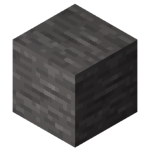
\includegraphics[width=4cm,height=\textheight,keepaspectratio,alt={Zeichnungstyp normal}]{bilder/drawtype_normal.png}
\caption{Zeichnungstyp normal}
\end{figure}

Der Zeichnungstyp \texttt{normal} wird typischerweise für würfelförmige
Nodes verwendet. Liegt eine Seite eines normalen Nodes an einer festen
Seite an, wird sie nicht gezeichnet. Das bringt einen großen
Leistungsgewinn.

Der Zeichnungstyp \texttt{allfaces} zeichnet dagegen auch die
Innenseite, wenn sie an einem festen Node anliegt. Das eignet sich für
Nodes mit teilweise transparenten Seiten, etwa Blätter. Mit
\texttt{allfaces\_\allowbreak{}optional} können Benutzer das langsamere
Zeichnen abschalten; der Node verhält sich dann wie ein normaler Node.

\begin{Shaded}
\begin{Highlighting}[]
\VariableTok{core}\OperatorTok{.}\NormalTok{register\_node}\OperatorTok{(}\StringTok{"mymod:diamond"}\OperatorTok{,} \OperatorTok{\{}
    \VariableTok{description} \OperatorTok{=} \StringTok{"Alien{-}Diamant"}\OperatorTok{,}
    \VariableTok{tiles} \OperatorTok{=} \OperatorTok{\{} \StringTok{"mymod\_diamond.png"} \OperatorTok{\},}
    \VariableTok{groups} \OperatorTok{=} \OperatorTok{\{} \VariableTok{cracky} \OperatorTok{=} \DecValTok{3} \OperatorTok{\},}
\OperatorTok{\})}

\VariableTok{core}\OperatorTok{.}\NormalTok{register\_node}\OperatorTok{(}\StringTok{"default:leaves"}\OperatorTok{,} \OperatorTok{\{}
    \VariableTok{description} \OperatorTok{=} \StringTok{"Blätter"}\OperatorTok{,}
    \VariableTok{drawtype} \OperatorTok{=} \StringTok{"allfaces\_optional"}\OperatorTok{,}
    \VariableTok{tiles} \OperatorTok{=} \OperatorTok{\{} \StringTok{"default\_leaves.png"} \OperatorTok{\},}
\OperatorTok{\})}
\end{Highlighting}
\end{Shaded}

Hinweis: \texttt{normal} ist der Standard-Zeichnungstyp, du musst ihn
also nicht ausdrücklich angeben.

\section{Glasartige Nodes}\label{glasartige-nodes}

Der Unterschied zwischen glasartigen (\texttt{glasslike}) und normalen
Nodes: Steht ein glasartiger Node neben einem normalen, wird die
angrenzende Seite des normalen Nodes trotzdem gezeichnet. Das ist
nützlich, weil glasartige Nodes meist transparent sind -- mit dem
Zeichnungstyp \texttt{normal} könnte man sonst durch die Welt
hindurchsehen.

\begin{figure}
\centering
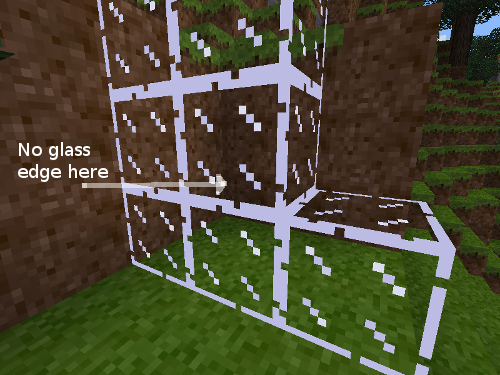
\includegraphics[width=7cm,height=\textheight,keepaspectratio,alt={Kanten bei glasslike}]{bilder/drawtype_glasslike_edges.png}
\caption{Kanten bei glasslike}
\end{figure}

\begin{Shaded}
\begin{Highlighting}[]
\VariableTok{core}\OperatorTok{.}\NormalTok{register\_node}\OperatorTok{(}\StringTok{"default:obsidian\_glass"}\OperatorTok{,} \OperatorTok{\{}
    \VariableTok{description} \OperatorTok{=} \StringTok{"Obsidianglas"}\OperatorTok{,}
    \VariableTok{drawtype} \OperatorTok{=} \StringTok{"glasslike"}\OperatorTok{,}
    \VariableTok{tiles} \OperatorTok{=} \OperatorTok{\{} \StringTok{"default\_obsidian\_glass.png"} \OperatorTok{\},}
    \VariableTok{paramtype} \OperatorTok{=} \StringTok{"light"}\OperatorTok{,}
    \VariableTok{is\_ground\_content} \OperatorTok{=} \KeywordTok{false}\OperatorTok{,}
    \VariableTok{sunlight\_propagates} \OperatorTok{=} \KeywordTok{true}\OperatorTok{,}
    \VariableTok{sounds} \OperatorTok{=} \VariableTok{default}\OperatorTok{.}\NormalTok{node\_sound\_glass\_defaults}\OperatorTok{(),}
    \VariableTok{groups} \OperatorTok{=} \OperatorTok{\{} \VariableTok{cracky} \OperatorTok{=} \DecValTok{3}\OperatorTok{,} \VariableTok{oddly\_breakable\_by\_hand} \OperatorTok{=} \DecValTok{3} \OperatorTok{\},}
\OperatorTok{\})}
\end{Highlighting}
\end{Shaded}

\subsection{glasslike\_framed}\label{glasslike_framed}

Hier läuft der Rand mit einem 3D-Effekt um die gesamte zusammenhängende
Fläche statt um jeden einzelnen Node:

\begin{figure}
\centering
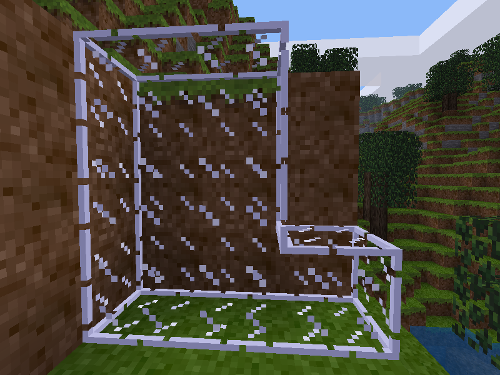
\includegraphics[width=7cm,height=\textheight,keepaspectratio,alt={Kanten bei glasslike\_framed}]{bilder/drawtype_glasslike_framed.png}
\caption{Kanten bei glasslike\_framed}
\end{figure}

Mit dem Zeichnungstyp
\texttt{glasslike\_\allowbreak{}framed\_\allowbreak{}optional} kann der
Benutzer das gerahmte Aussehen selbst \emph{einschalten}.

\begin{Shaded}
\begin{Highlighting}[]
\VariableTok{core}\OperatorTok{.}\NormalTok{register\_node}\OperatorTok{(}\StringTok{"default:glass"}\OperatorTok{,} \OperatorTok{\{}
    \VariableTok{description} \OperatorTok{=} \StringTok{"Glas"}\OperatorTok{,}
    \VariableTok{drawtype} \OperatorTok{=} \StringTok{"glasslike\_framed"}\OperatorTok{,}
    \VariableTok{tiles} \OperatorTok{=} \OperatorTok{\{}
        \StringTok{"default\_glass.png"}\OperatorTok{,}
        \StringTok{"default\_glass\_detail.png"}\OperatorTok{,}
    \OperatorTok{\},}
    \VariableTok{inventory\_image} \OperatorTok{=} \VariableTok{core}\OperatorTok{.}\NormalTok{inventorycube}\OperatorTok{(}
        \StringTok{"default\_glass.png"}
    \OperatorTok{),}
    \VariableTok{paramtype} \OperatorTok{=} \StringTok{"light"}\OperatorTok{,}
    \VariableTok{sunlight\_propagates} \OperatorTok{=} \KeywordTok{true}\OperatorTok{,} \CommentTok{{-}{-} Sonnenlicht geht durch}
    \VariableTok{groups} \OperatorTok{=} \OperatorTok{\{} \VariableTok{cracky} \OperatorTok{=} \DecValTok{3}\OperatorTok{,} \VariableTok{oddly\_breakable\_by\_hand} \OperatorTok{=} \DecValTok{3} \OperatorTok{\},}
    \VariableTok{sounds} \OperatorTok{=} \VariableTok{default}\OperatorTok{.}\NormalTok{node\_sound\_glass\_defaults}\OperatorTok{(),}
\OperatorTok{\})}
\end{Highlighting}
\end{Shaded}

\section{Luftartige Nodes}\label{luftartige-nodes}

Diese Nodes werden nicht gezeichnet und haben daher keine
Texturen.\index{textur@Textur}

\begin{Shaded}
\begin{Highlighting}[]
\VariableTok{core}\OperatorTok{.}\NormalTok{register\_node}\OperatorTok{(}\StringTok{"myair:air"}\OperatorTok{,} \OperatorTok{\{}
    \VariableTok{description} \OperatorTok{=} \StringTok{"MyAir (du Hacker, du!)"}\OperatorTok{,}
    \VariableTok{drawtype} \OperatorTok{=} \StringTok{"airlike"}\OperatorTok{,}
    \VariableTok{paramtype} \OperatorTok{=} \StringTok{"light"}\OperatorTok{,}
    \VariableTok{sunlight\_propagates} \OperatorTok{=} \KeywordTok{true}\OperatorTok{,}

    \VariableTok{walkable} \OperatorTok{=} \KeywordTok{false}\OperatorTok{,} \CommentTok{{-}{-} sonst kollidiert der Spieler}
    \VariableTok{pointable} \OperatorTok{=} \KeywordTok{false}\OperatorTok{,} \CommentTok{{-}{-} Node kann nicht ausgewählt werden}
    \VariableTok{diggable} \OperatorTok{=} \KeywordTok{false}\OperatorTok{,} \CommentTok{{-}{-} Node kann nicht abgebaut werden}
    \VariableTok{buildable\_to} \OperatorTok{=} \KeywordTok{true}\OperatorTok{,} \CommentTok{{-}{-} Nodes können diesen Node ersetzen}
    \CommentTok{{-}{-} (man kann einen Node an seine Stelle}
    \CommentTok{{-}{-} setzen, die Luft verschwindet dann)}

    \VariableTok{air\_equivalent} \OperatorTok{=} \KeywordTok{true}\OperatorTok{,}
    \VariableTok{drop} \OperatorTok{=} \StringTok{""}\OperatorTok{,}
    \VariableTok{groups} \OperatorTok{=} \OperatorTok{\{} \VariableTok{not\_in\_creative\_inventory} \OperatorTok{=} \DecValTok{1} \OperatorTok{\},}
\OperatorTok{\})}
\end{Highlighting}
\end{Shaded}

\section{Beleuchtung und Ausbreitung des
Sonnenlichts}\label{beleuchtung-und-ausbreitung-des-sonnenlichts}

Die Beleuchtung eines Nodes wird in \texttt{param1} gespeichert. Um zu
berechnen, wie eine Seite eines Nodes schattiert wird, nimmt Luanti den
Lichtwert des benachbarten Nodes. Deshalb haben feste Nodes keine
Lichtwerte -- sie blockieren das Licht ja.

Standardmäßig erlaubt ein Node-Typ nicht, Licht in seinen Instanzen zu
speichern. Bei manchen Nodes wie Glas und Luft soll Licht aber
durchgehen. Dazu müssen zwei Eigenschaften gesetzt werden:

\begin{Shaded}
\begin{Highlighting}[]
\VariableTok{paramtype} \OperatorTok{=} \StringTok{"light"}\OperatorTok{,}
\VariableTok{sunlight\_propagates} \OperatorTok{=} \KeywordTok{true}\OperatorTok{,}
\end{Highlighting}
\end{Shaded}

Die erste Zeile bedeutet, dass \texttt{param1} tatsächlich den Lichtwert
speichert. Die zweite, dass Sonnenlicht ohne Abschwächung durch den Node
hindurchgeht.

\section{Flüssige Nodes}\label{fluxfcssige-nodes}

\begin{figure}
\centering

\includegraphics[width=4cm,height=\textheight,keepaspectratio,alt={Zeichnungstyp liquid}]{bilder/drawtype_liquid.png}
\caption{Zeichnungstyp liquid}
\end{figure}

Jede Flüssigkeit braucht zwei Node-Definitionen: eine für die Quelle und
eine für die fließende Flüssigkeit.

\begin{Shaded}
\begin{Highlighting}[]
\CommentTok{{-}{-} Einige Eigenschaften wurden weggelassen, weil sie über}
\CommentTok{{-}{-} dieses Kapitel hinausgehen.}
\VariableTok{core}\OperatorTok{.}\NormalTok{register\_node}\OperatorTok{(}\StringTok{"default:water\_source"}\OperatorTok{,} \OperatorTok{\{}
    \VariableTok{drawtype} \OperatorTok{=} \StringTok{"liquid"}\OperatorTok{,}
    \VariableTok{paramtype} \OperatorTok{=} \StringTok{"light"}\OperatorTok{,}

    \VariableTok{inventory\_image} \OperatorTok{=} \VariableTok{core}\OperatorTok{.}\NormalTok{inventorycube}\OperatorTok{(}
        \StringTok{"default\_water.png"}
    \OperatorTok{),}
    \CommentTok{{-}{-} \^{} nötig, damit das Inventarbild nicht animiert wird}

    \VariableTok{tiles} \OperatorTok{=} \OperatorTok{\{}
        \OperatorTok{\{}
            \VariableTok{name} \OperatorTok{=} \StringTok{"default\_water\_source\_animated.png"}\OperatorTok{,}
            \VariableTok{animation} \OperatorTok{=} \OperatorTok{\{}
                \FunctionTok{type} \OperatorTok{=} \StringTok{"vertical\_frames"}\OperatorTok{,}
                \VariableTok{aspect\_w} \OperatorTok{=} \DecValTok{16}\OperatorTok{,}
                \VariableTok{aspect\_h} \OperatorTok{=} \DecValTok{16}\OperatorTok{,}
                \VariableTok{length} \OperatorTok{=} \DecValTok{2.0}\OperatorTok{,}
            \OperatorTok{\},}
        \OperatorTok{\},}
    \OperatorTok{\},}

    \VariableTok{special\_tiles} \OperatorTok{=} \OperatorTok{\{}
        \CommentTok{{-}{-} Wasserquellen neuen Typs (kaum genutzt)}
        \OperatorTok{\{}
            \VariableTok{name} \OperatorTok{=} \StringTok{"default\_water\_source\_animated.png"}\OperatorTok{,}
            \VariableTok{animation} \OperatorTok{=} \OperatorTok{\{}
                \FunctionTok{type} \OperatorTok{=} \StringTok{"vertical\_frames"}\OperatorTok{,}
                \VariableTok{aspect\_w} \OperatorTok{=} \DecValTok{16}\OperatorTok{,}
                \VariableTok{aspect\_h} \OperatorTok{=} \DecValTok{16}\OperatorTok{,}
                \VariableTok{length} \OperatorTok{=} \DecValTok{2.0}\OperatorTok{,}
            \OperatorTok{\},}
            \VariableTok{backface\_culling} \OperatorTok{=} \KeywordTok{false}\OperatorTok{,}
        \OperatorTok{\},}
    \OperatorTok{\},}

    \CommentTok{{-}{-}}
    \CommentTok{{-}{-} Verhalten}
    \CommentTok{{-}{-}}
    \VariableTok{walkable} \OperatorTok{=} \KeywordTok{false}\OperatorTok{,} \CommentTok{{-}{-} Spieler fällt hindurch}
    \VariableTok{pointable} \OperatorTok{=} \KeywordTok{false}\OperatorTok{,} \CommentTok{{-}{-} Spieler kann es nicht auswählen}
    \VariableTok{diggable} \OperatorTok{=} \KeywordTok{false}\OperatorTok{,} \CommentTok{{-}{-} Spieler kann es nicht abbauen}
    \VariableTok{buildable\_to} \OperatorTok{=} \KeywordTok{true}\OperatorTok{,} \CommentTok{{-}{-} Nodes können diesen Node ersetzen}

    \VariableTok{alpha} \OperatorTok{=} \DecValTok{160}\OperatorTok{,}

    \CommentTok{{-}{-}}
    \CommentTok{{-}{-} Flüssigkeitseigenschaften}
    \CommentTok{{-}{-}}
    \VariableTok{drowning} \OperatorTok{=} \DecValTok{1}\OperatorTok{,}
    \VariableTok{liquidtype} \OperatorTok{=} \StringTok{"source"}\OperatorTok{,}

    \VariableTok{liquid\_alternative\_flowing} \OperatorTok{=} \StringTok{"default:water\_flowing"}\OperatorTok{,}
    \CommentTok{{-}{-} \^{} wenn die Flüssigkeit fließt}

    \VariableTok{liquid\_alternative\_source} \OperatorTok{=} \StringTok{"default:water\_source"}\OperatorTok{,}
    \CommentTok{{-}{-} \^{} wenn die Flüssigkeit eine Quelle ist}

    \VariableTok{liquid\_viscosity} \OperatorTok{=} \ConstantTok{WATER\_VISC}\OperatorTok{,}
    \CommentTok{{-}{-} \^{} wie schnell}

    \VariableTok{liquid\_range} \OperatorTok{=} \DecValTok{8}\OperatorTok{,}
    \CommentTok{{-}{-} \^{} wie weit}

    \VariableTok{post\_effect\_color} \OperatorTok{=} \OperatorTok{\{} \VariableTok{a} \OperatorTok{=} \DecValTok{64}\OperatorTok{,} \VariableTok{r} \OperatorTok{=} \DecValTok{100}\OperatorTok{,} \VariableTok{g} \OperatorTok{=} \DecValTok{100}\OperatorTok{,} \VariableTok{b} \OperatorTok{=} \DecValTok{200} \OperatorTok{\},}
    \CommentTok{{-}{-} \^{} Bildschirmfarbe unter Wasser}
\OperatorTok{\})}
\end{Highlighting}
\end{Shaded}

Fließende Nodes werden ähnlich definiert, nur mit anderem Namen und
anderer Animation. Ein vollständiges Beispiel ist
\texttt{default:water\_\allowbreak{}flowing} im Mod \texttt{default} von
Minetest Game.

\section{Nodeboxen}\label{nodeboxen}

\begin{figure}
\centering
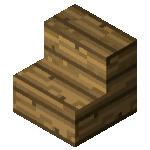
\includegraphics[width=4cm,height=\textheight,keepaspectratio,alt={Zeichnungstyp nodebox}]{bilder/drawtype_nodebox.png}
\caption{Zeichnungstyp nodebox}
\end{figure}

Mit Nodeboxen\index{nodebox@Nodebox} erstellst du Nodes, die nicht
würfelförmig sind, sondern aus beliebig vielen Quadern bestehen.

\begin{Shaded}
\begin{Highlighting}[]
\VariableTok{core}\OperatorTok{.}\NormalTok{register\_node}\OperatorTok{(}\StringTok{"stairs:stair\_stone"}\OperatorTok{,} \OperatorTok{\{}
    \VariableTok{drawtype} \OperatorTok{=} \StringTok{"nodebox"}\OperatorTok{,}
    \VariableTok{paramtype} \OperatorTok{=} \StringTok{"light"}\OperatorTok{,}
    \VariableTok{node\_box} \OperatorTok{=} \OperatorTok{\{}
        \FunctionTok{type} \OperatorTok{=} \StringTok{"fixed"}\OperatorTok{,}
        \VariableTok{fixed} \OperatorTok{=} \OperatorTok{\{}
            \OperatorTok{\{} \OperatorTok{{-}}\DecValTok{0.5}\OperatorTok{,} \OperatorTok{{-}}\DecValTok{0.5}\OperatorTok{,} \OperatorTok{{-}}\DecValTok{0.5}\OperatorTok{,} \DecValTok{0.5}\OperatorTok{,} \DecValTok{0}\OperatorTok{,} \DecValTok{0.5} \OperatorTok{\},}
            \OperatorTok{\{} \OperatorTok{{-}}\DecValTok{0.5}\OperatorTok{,} \DecValTok{0}\OperatorTok{,} \DecValTok{0}\OperatorTok{,} \DecValTok{0.5}\OperatorTok{,} \DecValTok{0.5}\OperatorTok{,} \DecValTok{0.5} \OperatorTok{\},}
        \OperatorTok{\},}
    \OperatorTok{\},}
\OperatorTok{\})}
\end{Highlighting}
\end{Shaded}

Der wichtigste Teil ist die Nodebox-Tabelle:

\begin{Shaded}
\begin{Highlighting}[]
\OperatorTok{\{{-}}\DecValTok{0.5}\OperatorTok{,} \OperatorTok{{-}}\DecValTok{0.5}\OperatorTok{,} \OperatorTok{{-}}\DecValTok{0.5}\OperatorTok{,}       \DecValTok{0.5}\OperatorTok{,}    \DecValTok{0}\OperatorTok{,}  \DecValTok{0.5}\OperatorTok{\},}
\OperatorTok{\{{-}}\DecValTok{0.5}\OperatorTok{,}    \DecValTok{0}\OperatorTok{,}    \DecValTok{0}\OperatorTok{,}       \DecValTok{0.5}\OperatorTok{,}  \DecValTok{0.5}\OperatorTok{,}  \DecValTok{0.5}\OperatorTok{\}}
\end{Highlighting}
\end{Shaded}

Jede Zeile ist ein Quader; zusammen ergeben sie einen einzigen Node. Die
ersten drei Zahlen sind die Koordinaten (von −0,5 bis einschließlich
0,5) der unteren, vorderen, linken Ecke, die letzten drei die der
gegenüberliegenden Ecke. Die Reihenfolge ist X, Y, Z, wobei Y nach oben
zeigt.

Mit dem NodeBoxEditor\footnote{\url{https://forum.luanti.org/viewtopic.php?f=14&t=2840}}
kannst du Nodeboxen erstellen, indem du die Kanten ziehst. Das ist
anschaulicher als die Arbeit von Hand.

\subsection{Nodeboxen für
Wandmontage}\label{nodeboxen-fuxfcr-wandmontage}

Manchmal braucht man unterschiedliche Nodeboxen, je nachdem, ob der Node
auf dem Boden, an der Wand oder an der Decke platziert wird, etwa bei
Fackeln.

\begin{Shaded}
\begin{Highlighting}[]
\VariableTok{core}\OperatorTok{.}\NormalTok{register\_node}\OperatorTok{(}\StringTok{"default:sign\_wall"}\OperatorTok{,} \OperatorTok{\{}
    \VariableTok{drawtype} \OperatorTok{=} \StringTok{"nodebox"}\OperatorTok{,}
    \VariableTok{node\_box} \OperatorTok{=} \OperatorTok{\{}
        \FunctionTok{type} \OperatorTok{=} \StringTok{"wallmounted"}\OperatorTok{,}

        \CommentTok{{-}{-} Decke}
        \VariableTok{wall\_top} \OperatorTok{=} \OperatorTok{\{}
            \OperatorTok{\{}
                \OperatorTok{{-}}\DecValTok{0.4375}\OperatorTok{,}
                \DecValTok{0.4375}\OperatorTok{,}
                \OperatorTok{{-}}\DecValTok{0.3125}\OperatorTok{,}
                \DecValTok{0.4375}\OperatorTok{,}
                \DecValTok{0.5}\OperatorTok{,}
                \DecValTok{0.3125}\OperatorTok{,}
            \OperatorTok{\},}
        \OperatorTok{\},}

        \CommentTok{{-}{-} Boden}
        \VariableTok{wall\_bottom} \OperatorTok{=} \OperatorTok{\{}
            \OperatorTok{\{}
                \OperatorTok{{-}}\DecValTok{0.4375}\OperatorTok{,}
                \OperatorTok{{-}}\DecValTok{0.5}\OperatorTok{,}
                \OperatorTok{{-}}\DecValTok{0.3125}\OperatorTok{,}
                \DecValTok{0.4375}\OperatorTok{,}
                \OperatorTok{{-}}\DecValTok{0.4375}\OperatorTok{,}
                \DecValTok{0.3125}\OperatorTok{,}
            \OperatorTok{\},}
        \OperatorTok{\},}

        \CommentTok{{-}{-} Wand}
        \VariableTok{wall\_side} \OperatorTok{=} \OperatorTok{\{}
            \OperatorTok{\{}
                \OperatorTok{{-}}\DecValTok{0.5}\OperatorTok{,}
                \OperatorTok{{-}}\DecValTok{0.3125}\OperatorTok{,}
                \OperatorTok{{-}}\DecValTok{0.4375}\OperatorTok{,}
                \OperatorTok{{-}}\DecValTok{0.4375}\OperatorTok{,}
                \DecValTok{0.3125}\OperatorTok{,}
                \DecValTok{0.4375}\OperatorTok{,}
            \OperatorTok{\},}
        \OperatorTok{\},}
    \OperatorTok{\},}
\OperatorTok{\})}
\end{Highlighting}
\end{Shaded}

\section{Mesh-Nodes}\label{mesh-nodes}

Nodeboxen sind zwar meist einfacher zu erstellen, bestehen aber nur aus
Quadern. Außerdem sind sie nicht optimiert: Innenflächen werden auch
dann gezeichnet, wenn sie vollständig verdeckt sind.

Eine Fläche (\emph{face}) ist eine ebene Oberfläche eines Meshs. Eine
Innenfläche entsteht, wenn sich die Flächen zweier Nodeboxen überlappen.
Teile des Modells sind dann unsichtbar, werden aber trotzdem gezeichnet.

So registrierst du einen Mesh-Node:

\begin{Shaded}
\begin{Highlighting}[]
\VariableTok{core}\OperatorTok{.}\NormalTok{register\_node}\OperatorTok{(}\StringTok{"mymod:meshy"}\OperatorTok{,} \OperatorTok{\{}
    \VariableTok{drawtype} \OperatorTok{=} \StringTok{"mesh"}\OperatorTok{,}

    \CommentTok{{-}{-} Enthält die Textur für jedes „Material“}
    \VariableTok{tiles} \OperatorTok{=} \OperatorTok{\{}
        \StringTok{"mymod\_meshy.png"}\OperatorTok{,}
    \OperatorTok{\},}

    \CommentTok{{-}{-} Pfad zum Mesh}
    \VariableTok{mesh} \OperatorTok{=} \StringTok{"mymod\_meshy.b3d"}\OperatorTok{,}
\OperatorTok{\})}
\end{Highlighting}
\end{Shaded}

Achte darauf, dass das Mesh\index{mesh@Mesh} in einem Verzeichnis
\texttt{models} liegt. Meist gehört es in den Ordner deines eigenen
Mods; du kannst aber auch ein Mesh aus einem anderen Mod verwenden, von
dem deiner abhängt. Ein Mod, der weitere Möbel hinzufügt, kann zum
Beispiel die Modelle eines grundlegenden Möbel-Mods mitnutzen.

\section{Signlike-Nodes}\label{signlike-nodes}

Signlike-Nodes sind flache Nodes, die an den Seiten anderer Nodes
angebracht werden. Trotz des Namens verwenden Schilder meist nicht
\texttt{signlike}, sondern \texttt{nodebox}, um einen 3D-Effekt zu
erzielen. Leitern dagegen nutzen häufig \texttt{signlike}.

\begin{Shaded}
\begin{Highlighting}[]
\VariableTok{core}\OperatorTok{.}\NormalTok{register\_node}\OperatorTok{(}\StringTok{"default:ladder\_wood"}\OperatorTok{,} \OperatorTok{\{}
    \VariableTok{drawtype} \OperatorTok{=} \StringTok{"signlike"}\OperatorTok{,}

    \VariableTok{tiles} \OperatorTok{=} \OperatorTok{\{} \StringTok{"default\_ladder\_wood.png"} \OperatorTok{\},}

    \CommentTok{{-}{-} Erforderlich: Drehung in param2 speichern}
    \VariableTok{paramtype2} \OperatorTok{=} \StringTok{"wallmounted"}\OperatorTok{,}

    \VariableTok{selection\_box} \OperatorTok{=} \OperatorTok{\{}
        \FunctionTok{type} \OperatorTok{=} \StringTok{"wallmounted"}\OperatorTok{,}
    \OperatorTok{\},}
\OperatorTok{\})}
\end{Highlighting}
\end{Shaded}

\section{Plantlike-Nodes}\label{plantlike-nodes}

\begin{figure}
\centering

\includegraphics[width=4cm,height=\textheight,keepaspectratio,alt={Zeichnungstyp plantlike}]{bilder/drawtype_plantlike.png}
\caption{Zeichnungstyp plantlike}
\end{figure}

Plantlike-Nodes zeichnen ihre Textur in einem X-förmigen Muster.

\begin{Shaded}
\begin{Highlighting}[]
\VariableTok{core}\OperatorTok{.}\NormalTok{register\_node}\OperatorTok{(}\StringTok{"default:papyrus"}\OperatorTok{,} \OperatorTok{\{}
    \VariableTok{drawtype} \OperatorTok{=} \StringTok{"plantlike"}\OperatorTok{,}

    \CommentTok{{-}{-} Nur eine Textur}
    \VariableTok{tiles} \OperatorTok{=} \OperatorTok{\{} \StringTok{"default\_papyrus.png"} \OperatorTok{\},}

    \VariableTok{selection\_box} \OperatorTok{=} \OperatorTok{\{}
        \FunctionTok{type} \OperatorTok{=} \StringTok{"fixed"}\OperatorTok{,}
        \VariableTok{fixed} \OperatorTok{=} \OperatorTok{\{}
            \OperatorTok{{-}}\DecValTok{6} \OperatorTok{/} \DecValTok{16}\OperatorTok{,}
            \OperatorTok{{-}}\DecValTok{0.5}\OperatorTok{,}
            \OperatorTok{{-}}\DecValTok{6} \OperatorTok{/} \DecValTok{16}\OperatorTok{,}
            \DecValTok{6} \OperatorTok{/} \DecValTok{16}\OperatorTok{,}
            \DecValTok{0.5}\OperatorTok{,}
            \DecValTok{6} \OperatorTok{/} \DecValTok{16}\OperatorTok{,}
        \OperatorTok{\},}
    \OperatorTok{\},}
\OperatorTok{\})}
\end{Highlighting}
\end{Shaded}

\section{Firelike-Nodes}\label{firelike-nodes}

\texttt{firelike} ähnelt \texttt{plantlike}, ist aber so gestaltet, dass
es an Wänden und Decken „haftet``.

\begin{figure}
\centering
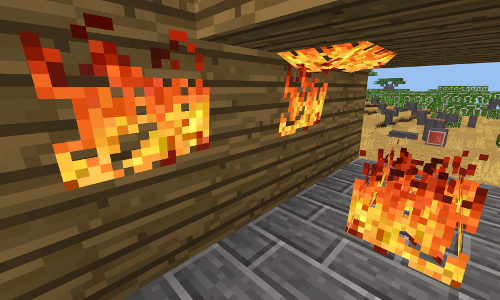
\includegraphics[width=7cm,height=\textheight,keepaspectratio,alt={Firelike-Nodes}]{bilder/drawtype_firelike.png}
\caption{Firelike-Nodes}
\end{figure}

\begin{Shaded}
\begin{Highlighting}[]
\VariableTok{core}\OperatorTok{.}\NormalTok{register\_node}\OperatorTok{(}\StringTok{"mymod:clinger"}\OperatorTok{,} \OperatorTok{\{}
    \VariableTok{drawtype} \OperatorTok{=} \StringTok{"firelike"}\OperatorTok{,}

    \CommentTok{{-}{-} Nur eine Textur}
    \VariableTok{tiles} \OperatorTok{=} \OperatorTok{\{} \StringTok{"mymod\_clinger.png"} \OperatorTok{\},}
\OperatorTok{\})}
\end{Highlighting}
\end{Shaded}

\section{Weitere Zeichnungstypen}\label{weitere-zeichnungstypen}

Die Liste ist nicht vollständig; es gibt noch weitere Typen, darunter:

\begin{itemize}
\tightlist
\item
  \texttt{fencelike}
\item
  \texttt{plantlike\_\allowbreak{}rooted} -- für Unterwasserpflanzen
\item
  \texttt{raillike} -- für Schienen
\item
  \texttt{torchlike} -- für 2D-Nodes an Wand, Boden oder Decke. Die
  Fackeln in Minetest Game verwenden allerdings Mesh-Nodes mit drei
  getrennten Definitionen (\texttt{default:torch},
  \texttt{default:torch\_\allowbreak{}wall} und
  \texttt{default:torch\_\allowbreak{}ceiling}).
\end{itemize}

Die vollständige Liste findest du wie immer in der
Lua-API-Dokumentation\footnote{\url{https://api.luanti.org/nodes/\#node-drawtypes}}.

\chapter{ItemStacks und Inventare}
\label{ch:items/inventories}

In diesem Kapitel lernst du, wie man Inventare\index{inventar@Inventar}
verwendet und verändert -- egal ob Spielerinventar, Node-Inventar oder
freistehendes Inventar.

\section{Was sind ItemStacks und
Inventare?}\label{was-sind-itemstacks-und-inventare}

Ein ItemStack\index{itemstack@\texttt{ItemStack}} sind die Daten hinter
einem einzelnen Feld eines Inventars.

Ein \emph{Inventar} ist eine Sammlung von \emph{Inventarlisten}, von
denen jede ein 2D-Gitter aus ItemStacks ist. Im Zusammenhang mit
Inventaren heißen Inventarlisten einfach \emph{Listen}.

Spieler und Nodes haben jeweils nur ein einziges Inventar; Listen
erlauben mehrere Gitter innerhalb dieses Inventars. Standardmäßig hat
der Spieler die Liste \texttt{main} für den Großteil seines Inventars
und einige Listen für das Crafting.

\section{ItemStacks}\label{itemstacks}

ItemStacks bestehen aus vier Teilen: \texttt{name}, \texttt{count},
\texttt{wear} und Metadaten.\index{metadaten@Metadaten}

Der Itemname kann der Name eines registrierten Items, ein
Alias\index{alias@Alias} oder ein unbekannter Itemname sein. Unbekannte
Items entstehen häufig, wenn Benutzer Mods deinstallieren oder Mods
Items ohne Vorkehrungen wie Aliase entfernen.

\begin{Shaded}
\begin{Highlighting}[]
\FunctionTok{print}\OperatorTok{(}\VariableTok{stack}\OperatorTok{:}\NormalTok{get\_name}\OperatorTok{())}
\VariableTok{stack}\OperatorTok{:}\NormalTok{set\_name}\OperatorTok{(}\StringTok{"default:dirt"}\OperatorTok{)}

\ControlFlowTok{if} \KeywordTok{not} \VariableTok{stack}\OperatorTok{:}\NormalTok{is\_known}\OperatorTok{()} \ControlFlowTok{then}
    \FunctionTok{print}\OperatorTok{(}\StringTok{"Unbekanntes Item!"}\OperatorTok{)}
\ControlFlowTok{end}
\end{Highlighting}
\end{Shaded}

Die Anzahl ist immer 0 oder größer. Im normalen Spielverlauf sollte sie
die maximale Stapelgröße des Items, \texttt{stack\_\allowbreak{}max},
nicht überschreiten. Admin-Befehle und fehlerhafte Mods können aber dazu
führen, dass Stacks größer werden.

\begin{Shaded}
\begin{Highlighting}[]
\FunctionTok{print}\OperatorTok{(}\VariableTok{stack}\OperatorTok{:}\NormalTok{get\_stack\_max}\OperatorTok{())}
\end{Highlighting}
\end{Shaded}

Ein ItemStack kann leer sein; dann ist die Anzahl 0.

\begin{Shaded}
\begin{Highlighting}[]
\FunctionTok{print}\OperatorTok{(}\VariableTok{stack}\OperatorTok{:}\NormalTok{get\_count}\OperatorTok{())}
\VariableTok{stack}\OperatorTok{:}\NormalTok{set\_count}\OperatorTok{(}\DecValTok{10}\OperatorTok{)}
\end{Highlighting}
\end{Shaded}

ItemStacks lassen sich mit der Funktion \texttt{ItemStack} auf
verschiedene Weise erzeugen:

\begin{Shaded}
\begin{Highlighting}[]
\NormalTok{ItemStack}\OperatorTok{()} \CommentTok{{-}{-} name="", count=0}
\NormalTok{ItemStack}\OperatorTok{(}\StringTok{"default:pick\_stone"}\OperatorTok{)} \CommentTok{{-}{-} count=1}
\NormalTok{ItemStack}\OperatorTok{(}\StringTok{"default:stone 30"}\OperatorTok{)}
\NormalTok{ItemStack}\OperatorTok{(\{} \VariableTok{name} \OperatorTok{=} \StringTok{"default:wood"}\OperatorTok{,} \VariableTok{count} \OperatorTok{=} \DecValTok{10} \OperatorTok{\})}
\end{Highlighting}
\end{Shaded}

Item-Metadaten sind ein unbegrenzter Schlüssel-Wert-Speicher für Daten
zum Item. Schlüssel-Wert heißt: Über einen Namen (den Schlüssel,
\emph{key}) greifst du auf die Daten (den Wert, \emph{value}) zu. Manche
Schlüssel haben eine besondere Bedeutung, etwa \texttt{description}, mit
dem ein Stack eine eigene Beschreibung bekommt. Mehr dazu im Kapitel
Speicherung und Metadaten~(Kapitel~\ref{ch:map/storage}).

\section{Inventarorte}\label{inventarorte}

Der Inventarort legt fest, wo und wie ein Inventar gespeichert wird. Es
gibt drei Arten: Spieler, Node und freistehend. Ein Inventar ist fest an
genau einen Ort gebunden -- Änderungen am Inventar wirken sofort.

\subsection{Node-Inventare}\label{node-inventare}

Node-Inventare gehören zur Position eines bestimmten Nodes, etwa einer
Truhe. Der Node muss geladen sein, weil das Inventar in den
Node-Metadaten~(Kapitel~\ref{ch:map/storage}) gespeichert wird.

\begin{Shaded}
\begin{Highlighting}[]
\VariableTok{on\_punch} \OperatorTok{=} \KeywordTok{function}\OperatorTok{(}\VariableTok{pos}\OperatorTok{,} \VariableTok{node}\OperatorTok{)}
    \KeywordTok{local} \VariableTok{inv} \OperatorTok{=}
        \VariableTok{core}\OperatorTok{.}\NormalTok{get\_inventory}\OperatorTok{(\{} \FunctionTok{type} \OperatorTok{=} \StringTok{"node"}\OperatorTok{,} \VariableTok{pos} \OperatorTok{=} \VariableTok{pos} \OperatorTok{\})}
    \CommentTok{{-}{-} jetzt das Inventar verwenden}
\KeywordTok{end}\OperatorTok{,}
\end{Highlighting}
\end{Shaded}

So erhältst du eine \emph{Inventar-Referenz}, meist \emph{InvRef}
genannt. Mit Inventar-Referenzen veränderst du ein Inventar.
\emph{Referenz} bedeutet, dass die Daten nicht im Objekt selbst liegen;
das Objekt ändert die Daten direkt an Ort und Stelle.

Den Ort einer Inventar-Referenz ermittelst du so:

\begin{Shaded}
\begin{Highlighting}[]
\KeywordTok{local} \VariableTok{location} \OperatorTok{=} \VariableTok{inv}\OperatorTok{:}\NormalTok{get\_location}\OperatorTok{()}
\end{Highlighting}
\end{Shaded}

\subsection{Spielerinventare}\label{spielerinventare}

Spielerinventare erhältst du auf ähnliche Weise oder über eine
Spieler-Referenz. Der Spieler muss online sein, damit du auf sein
Inventar zugreifen kannst.

\begin{Shaded}
\begin{Highlighting}[]
\KeywordTok{local} \VariableTok{inv} \OperatorTok{=} \VariableTok{core}\OperatorTok{.}\NormalTok{get\_inventory}\OperatorTok{(\{}
    \FunctionTok{type} \OperatorTok{=} \StringTok{"player"}\OperatorTok{,}
    \VariableTok{name} \OperatorTok{=} \StringTok{"player1"}\OperatorTok{,}
\OperatorTok{\})}
\CommentTok{{-}{-} oder}
\KeywordTok{local} \VariableTok{inv} \OperatorTok{=} \VariableTok{player}\OperatorTok{:}\NormalTok{get\_inventory}\OperatorTok{()}
\end{Highlighting}
\end{Shaded}

\subsection{Freistehende Inventare}\label{freistehende-inventare}

Ein freistehendes Inventar (\emph{detached inventory}) ist unabhängig
von Spielern und Nodes. Es wird bei einem Neustart nicht gespeichert.

\begin{Shaded}
\begin{Highlighting}[]
\KeywordTok{local} \VariableTok{inv} \OperatorTok{=} \VariableTok{core}\OperatorTok{.}\NormalTok{get\_inventory}\OperatorTok{(\{}
    \FunctionTok{type} \OperatorTok{=} \StringTok{"detached"}\OperatorTok{,}
    \VariableTok{name} \OperatorTok{=} \StringTok{"inventory\_name"}\OperatorTok{,}
\OperatorTok{\})}
\end{Highlighting}
\end{Shaded}

Anders als die anderen Inventararten musst du ein freistehendes Inventar
erst anlegen, bevor du darauf zugreifst:

\begin{Shaded}
\begin{Highlighting}[]
\VariableTok{core}\OperatorTok{.}\NormalTok{create\_detached\_inventory}\OperatorTok{(}\StringTok{"inventory\_name"}\OperatorTok{)}
\end{Highlighting}
\end{Shaded}

\texttt{create\_\allowbreak{}detached\_\allowbreak{}inventory} nimmt
drei Argumente entgegen, von denen nur das erste -- der Inventarname --
Pflicht ist. Das zweite ist eine Tabelle mit
Callbacks,\index{callback@Callback} mit denen du steuerst, wie Spieler
mit dem Inventar umgehen können:

\begin{Shaded}
\begin{Highlighting}[]
\CommentTok{{-}{-} Freistehendes Inventar, in das man nur hineinlegen kann}
\VariableTok{core}\OperatorTok{.}\NormalTok{create\_detached\_inventory}\OperatorTok{(}\StringTok{"inventory\_name"}\OperatorTok{,} \OperatorTok{\{}
    \VariableTok{allow\_move} \OperatorTok{=} \KeywordTok{function}\OperatorTok{(}
        \VariableTok{inv}\OperatorTok{,}
        \VariableTok{from\_list}\OperatorTok{,}
        \VariableTok{from\_index}\OperatorTok{,}
        \VariableTok{to\_list}\OperatorTok{,}
        \VariableTok{to\_index}\OperatorTok{,}
        \VariableTok{count}\OperatorTok{,}
        \VariableTok{player}
    \OperatorTok{)}
        \ControlFlowTok{return} \VariableTok{count} \CommentTok{{-}{-} Verschieben erlauben}
    \KeywordTok{end}\OperatorTok{,}

    \VariableTok{allow\_put} \OperatorTok{=} \KeywordTok{function}\OperatorTok{(}
        \VariableTok{inv}\OperatorTok{,}
        \VariableTok{listname}\OperatorTok{,}
        \VariableTok{index}\OperatorTok{,}
        \VariableTok{stack}\OperatorTok{,}
        \VariableTok{player}
    \OperatorTok{)}
        \ControlFlowTok{return} \VariableTok{stack}\OperatorTok{:}\NormalTok{get\_count}\OperatorTok{()} \CommentTok{{-}{-} Hineinlegen erlauben}
    \KeywordTok{end}\OperatorTok{,}

    \VariableTok{allow\_take} \OperatorTok{=} \KeywordTok{function}\OperatorTok{(}
        \VariableTok{inv}\OperatorTok{,}
        \VariableTok{listname}\OperatorTok{,}
        \VariableTok{index}\OperatorTok{,}
        \VariableTok{stack}\OperatorTok{,}
        \VariableTok{player}
    \OperatorTok{)}
        \ControlFlowTok{return} \DecValTok{0} \CommentTok{{-}{-} Herausnehmen verbieten}
    \KeywordTok{end}\OperatorTok{,}

    \VariableTok{on\_put} \OperatorTok{=} \KeywordTok{function}\OperatorTok{(}\VariableTok{inv}\OperatorTok{,} \VariableTok{listname}\OperatorTok{,} \VariableTok{index}\OperatorTok{,} \VariableTok{stack}\OperatorTok{,} \VariableTok{player}\OperatorTok{)}
        \VariableTok{core}\OperatorTok{.}\NormalTok{chat\_send\_all}\OperatorTok{(}
            \VariableTok{player}\OperatorTok{:}\NormalTok{get\_player\_name}\OperatorTok{()}
                \OperatorTok{..} \StringTok{" hat "}
                \OperatorTok{..} \VariableTok{stack}\OperatorTok{:}\NormalTok{to\_string}\OperatorTok{()}
                \OperatorTok{..} \StringTok{" in die Spendenkiste gelegt, von "}
                \OperatorTok{..} \VariableTok{core}\OperatorTok{.}\NormalTok{pos\_to\_string}\OperatorTok{(}\VariableTok{player}\OperatorTok{:}\NormalTok{get\_pos}\OperatorTok{())}
        \OperatorTok{)}
    \KeywordTok{end}\OperatorTok{,}
\OperatorTok{\})}
\end{Highlighting}
\end{Shaded}

Berechtigungs-Callbacks -- also die mit \texttt{allow\_\allowbreak{}} am
Anfang -- geben die Anzahl der zu übertragenden Items zurück; 0
verhindert die Übertragung ganz.

Aktions-Callbacks -- die mit \texttt{on\_\allowbreak{}} am Anfang --
haben dagegen keinen Rückgabewert.

\section{Listen}\label{listen}

Mit Inventarlisten lassen sich mehrere Gitter an einem einzigen Ort
speichern. Das ist vor allem für Spieler nützlich, denn es gibt einige
Listen, die alle Spiele haben, etwa das Hauptinventar (\texttt{main})
und die Craftingfelder (\texttt{craft}).

\subsection{Größe und Breite}\label{gruxf6uxdfe-und-breite}

Listen haben eine Größe, also die Gesamtzahl der Felder, und eine
Breite, die nur intern in der Engine verwendet wird. Beim Anzeigen des
Inventars in einem Fenster spielt die Breite der Liste keine Rolle, weil
der Code des Fensters die Breite selbst festlegt.

\begin{Shaded}
\begin{Highlighting}[]
\ControlFlowTok{if} \VariableTok{inv}\OperatorTok{:}\NormalTok{set\_size}\OperatorTok{(}\StringTok{"main"}\OperatorTok{,} \DecValTok{32}\OperatorTok{)} \ControlFlowTok{then}
    \VariableTok{inv}\OperatorTok{:}\NormalTok{set\_width}\OperatorTok{(}\StringTok{"main"}\OperatorTok{,} \DecValTok{8}\OperatorTok{)}
    \FunctionTok{print}\OperatorTok{(}\StringTok{"Größe:  "} \OperatorTok{..} \VariableTok{inv}\OperatorTok{:}\NormalTok{get\_size}\OperatorTok{(}\StringTok{"main"}\OperatorTok{))}
    \FunctionTok{print}\OperatorTok{(}\StringTok{"Breite: "} \OperatorTok{..} \VariableTok{inv}\OperatorTok{:}\NormalTok{get\_width}\OperatorTok{(}\StringTok{"main"}\OperatorTok{))}
\ControlFlowTok{else}
    \FunctionTok{print}\OperatorTok{(}\StringTok{"Fehler: ungültige Liste oder Größe"}\OperatorTok{)}
\ControlFlowTok{end}
\end{Highlighting}
\end{Shaded}

\texttt{set\_\allowbreak{}size} schlägt fehl und gibt \texttt{false}
zurück, wenn der Listenname oder die Größe ungültig ist -- etwa wenn die
neue Größe zu klein für die Items ist, die gerade im Inventar liegen.

\subsection{Inhalt prüfen}\label{inhalt-pruxfcfen}

Mit \texttt{is\_\allowbreak{}empty} prüfst du, ob eine Liste überhaupt
Items enthält:

\begin{Shaded}
\begin{Highlighting}[]
\ControlFlowTok{if} \VariableTok{inv}\OperatorTok{:}\NormalTok{is\_empty}\OperatorTok{(}\StringTok{"main"}\OperatorTok{)} \ControlFlowTok{then}
    \FunctionTok{print}\OperatorTok{(}\StringTok{"Die Liste ist leer!"}\OperatorTok{)}
\ControlFlowTok{end}
\end{Highlighting}
\end{Shaded}

Mit \texttt{contains\_\allowbreak{}item} prüfst du, ob eine Liste ein
bestimmtes Item enthält:

\begin{Shaded}
\begin{Highlighting}[]
\ControlFlowTok{if} \VariableTok{inv}\OperatorTok{:}\NormalTok{contains\_item}\OperatorTok{(}\StringTok{"main"}\OperatorTok{,} \StringTok{"default:stone"}\OperatorTok{)} \ControlFlowTok{then}
    \FunctionTok{print}\OperatorTok{(}\StringTok{"Ich habe Stein gefunden!"}\OperatorTok{)}
\ControlFlowTok{end}
\end{Highlighting}
\end{Shaded}

\section{Inventare und ItemStacks
verändern}\label{inventare-und-itemstacks-veruxe4ndern}

\subsection{Zu einer Liste
hinzufügen}\label{zu-einer-liste-hinzufuxfcgen}

\texttt{add\_\allowbreak{}item} fügt Items zu einer Liste hinzu (hier
\texttt{\textquotedbl{}main\textquotedbl{}}). Im folgenden Beispiel wird
dabei auch die maximale Stapelgröße beachtet:

\begin{Shaded}
\begin{Highlighting}[]
\KeywordTok{local} \VariableTok{stack} \OperatorTok{=}\NormalTok{ ItemStack}\OperatorTok{(}\StringTok{"default:stone 99"}\OperatorTok{)}
\KeywordTok{local} \VariableTok{leftover} \OperatorTok{=} \VariableTok{inv}\OperatorTok{:}\NormalTok{add\_item}\OperatorTok{(}\StringTok{"main"}\OperatorTok{,} \VariableTok{stack}\OperatorTok{)}
\ControlFlowTok{if} \VariableTok{leftover}\OperatorTok{:}\NormalTok{get\_count}\OperatorTok{()} \OperatorTok{\textgreater{}} \DecValTok{0} \ControlFlowTok{then}
    \FunctionTok{print}\OperatorTok{(}
        \StringTok{"Inventar ist voll! "}
            \OperatorTok{..} \VariableTok{leftover}\OperatorTok{:}\NormalTok{get\_count}\OperatorTok{()}
            \OperatorTok{..} \StringTok{" Items wurden nicht hinzugefügt"}
    \OperatorTok{)}
\ControlFlowTok{end}
\end{Highlighting}
\end{Shaded}

\subsection{Items herausnehmen}\label{items-herausnehmen}

So entfernst du Items aus einer Liste:

\begin{Shaded}
\begin{Highlighting}[]
\KeywordTok{local} \VariableTok{taken} \OperatorTok{=} \VariableTok{inv}\OperatorTok{:}\NormalTok{remove\_item}\OperatorTok{(}\StringTok{"main"}\OperatorTok{,} \VariableTok{stack}\OperatorTok{)}
\FunctionTok{print}\OperatorTok{(}\StringTok{"Herausgenommen: "} \OperatorTok{..} \VariableTok{taken}\OperatorTok{:}\NormalTok{get\_count}\OperatorTok{())}
\end{Highlighting}
\end{Shaded}

\subsection{Stacks verändern}\label{stacks-veruxe4ndern}

Einzelne Stacks veränderst du, indem du sie zuerst holst:

\begin{Shaded}
\begin{Highlighting}[]
\KeywordTok{local} \VariableTok{stack} \OperatorTok{=} \VariableTok{inv}\OperatorTok{:}\NormalTok{get\_stack}\OperatorTok{(}\VariableTok{listname}\OperatorTok{,} \DecValTok{1}\OperatorTok{)}
\end{Highlighting}
\end{Shaded}

Dann änderst du sie, indem du Eigenschaften setzt oder Methoden
verwendest, die die Stapelgröße beachten:

\begin{Shaded}
\begin{Highlighting}[]
\KeywordTok{local} \VariableTok{stack} \OperatorTok{=}\NormalTok{ ItemStack}\OperatorTok{(}\StringTok{"default:stone 50"}\OperatorTok{)}
\KeywordTok{local} \VariableTok{to\_add} \OperatorTok{=}\NormalTok{ ItemStack}\OperatorTok{(}\StringTok{"default:stone 100"}\OperatorTok{)}
\KeywordTok{local} \VariableTok{leftover} \OperatorTok{=} \VariableTok{stack}\OperatorTok{:}\NormalTok{add\_item}\OperatorTok{(}\VariableTok{to\_add}\OperatorTok{)}
\KeywordTok{local} \VariableTok{taken} \OperatorTok{=} \VariableTok{stack}\OperatorTok{:}\NormalTok{take\_item}\OperatorTok{(}\DecValTok{19}\OperatorTok{)}

\FunctionTok{print}\OperatorTok{(}
    \StringTok{"Konnte "}
        \OperatorTok{..} \VariableTok{leftover}\OperatorTok{:}\NormalTok{get\_count}\OperatorTok{()}
        \OperatorTok{..} \StringTok{" Items nicht hinzufügen."}
\OperatorTok{)}
\CommentTok{{-}{-} \^{} ergibt 51}

\FunctionTok{print}\OperatorTok{(}\StringTok{"Habe "} \OperatorTok{..} \VariableTok{stack}\OperatorTok{:}\NormalTok{get\_count}\OperatorTok{()} \OperatorTok{..} \StringTok{" Items"}\OperatorTok{)}
\CommentTok{{-}{-} \^{} ergibt 80}
\CommentTok{{-}{-}   min(50+100, stack\_max) {-} 19 = 80}
\CommentTok{{-}{-}     mit stack\_max = 99}
\end{Highlighting}
\end{Shaded}

\texttt{add\_\allowbreak{}item} fügt einem ItemStack Items hinzu und
gibt alles zurück, was nicht hineingepasst hat.
\texttt{take\_\allowbreak{}item} nimmt höchstens die angegebene Anzahl
heraus, eventuell auch weniger, und gibt den herausgenommenen Stack
zurück.

Zum Schluss setzt du den ItemStack wieder ein:

\begin{Shaded}
\begin{Highlighting}[]
\VariableTok{inv}\OperatorTok{:}\NormalTok{set\_stack}\OperatorTok{(}\VariableTok{listname}\OperatorTok{,} \DecValTok{1}\OperatorTok{,} \VariableTok{stack}\OperatorTok{)}
\end{Highlighting}
\end{Shaded}

Die Felder einer Liste werden, wie in Lua üblich, ab 1 gezählt.

\section{Abnutzung}\label{abnutzung}

Werkzeuge können sich abnutzen. Die Abnutzung\index{abnutzung@Abnutzung}
wird als Balken angezeigt, und ist das Werkzeug vollständig abgenutzt,
zerbricht es. Die Abnutzung ist eine Zahl bis 65535; je höher sie ist,
desto stärker ist das Werkzeug abgenutzt.

Du veränderst sie mit \texttt{add\_\allowbreak{}wear()},
\texttt{get\_\allowbreak{}wear()} und
\texttt{set\_\allowbreak{}wear(wear)}.

\begin{Shaded}
\begin{Highlighting}[]
\KeywordTok{local} \VariableTok{stack} \OperatorTok{=}\NormalTok{ ItemStack}\OperatorTok{(}\StringTok{"default:pick\_mese"}\OperatorTok{)}
\KeywordTok{local} \VariableTok{max\_uses} \OperatorTok{=} \DecValTok{10}

\CommentTok{{-}{-} Passiert automatisch beim Abbauen mit einem Werkzeug:}
\CommentTok{{-}{-} erhöht die Abnutzung um eine Benutzung.}
\VariableTok{stack}\OperatorTok{:}\NormalTok{add\_wear}\OperatorTok{(}\DecValTok{65535} \OperatorTok{/} \OperatorTok{(}\VariableTok{max\_uses} \OperatorTok{{-}} \DecValTok{1}\OperatorTok{))}
\end{Highlighting}
\end{Shaded}

Beim Abbauen kann die Abnutzung eines Werkzeugs vom abgebauten Node
abhängen; \texttt{max\_\allowbreak{}uses} ist also je nach Node
verschieden.

\section{Lua-Tabellen}\label{lua-tabellen}

ItemStacks und Inventare lassen sich in Tabellen umwandeln und
umgekehrt. Das ist praktisch zum Kopieren und für Massenoperationen.

\begin{Shaded}
\begin{Highlighting}[]
\CommentTok{{-}{-} Ganzes Inventar}
\KeywordTok{local} \VariableTok{data} \OperatorTok{=} \VariableTok{inv1}\OperatorTok{:}\NormalTok{get\_lists}\OperatorTok{()}
\VariableTok{inv2}\OperatorTok{:}\NormalTok{set\_lists}\OperatorTok{(}\VariableTok{data}\OperatorTok{)}

\CommentTok{{-}{-} Eine Liste}
\KeywordTok{local} \VariableTok{listdata} \OperatorTok{=} \VariableTok{inv1}\OperatorTok{:}\NormalTok{get\_list}\OperatorTok{(}\StringTok{"main"}\OperatorTok{)}
\VariableTok{inv2}\OperatorTok{:}\NormalTok{set\_list}\OperatorTok{(}\StringTok{"main"}\OperatorTok{,} \VariableTok{listdata}\OperatorTok{)}
\end{Highlighting}
\end{Shaded}

Die von \texttt{get\_\allowbreak{}lists()} zurückgegebene Tabelle sieht
so aus:

\begin{Shaded}
\begin{Highlighting}[]
\OperatorTok{\{}
    \VariableTok{list\_one} \OperatorTok{=} \OperatorTok{\{}
        \VariableTok{ItemStack}\OperatorTok{,}
        \VariableTok{ItemStack}\OperatorTok{,}
        \VariableTok{ItemStack}\OperatorTok{,}
        \VariableTok{ItemStack}\OperatorTok{,}
        \CommentTok{{-}{-} inv:get\_size("list\_one") Elemente}
    \OperatorTok{\},}
    \VariableTok{list\_two} \OperatorTok{=} \OperatorTok{\{}
        \VariableTok{ItemStack}\OperatorTok{,}
        \VariableTok{ItemStack}\OperatorTok{,}
        \VariableTok{ItemStack}\OperatorTok{,}
        \VariableTok{ItemStack}\OperatorTok{,}
        \CommentTok{{-}{-} inv:get\_size("list\_two") Elemente}
    \OperatorTok{\},}
\OperatorTok{\},}
\end{Highlighting}
\end{Shaded}

\texttt{get\_\allowbreak{}list()} gibt eine einzelne Liste zurück, also
einfach eine Liste von ItemStacks.

Wichtig: Die \texttt{set}-Methoden oben verändern die Größe der Listen
nicht. Du kannst eine Liste also leeren, indem du sie auf eine leere
Tabelle setzt, ohne dass sie kleiner wird:

\begin{Shaded}
\begin{Highlighting}[]
\VariableTok{inv}\OperatorTok{:}\NormalTok{set\_list}\OperatorTok{(}\StringTok{"main"}\OperatorTok{,} \OperatorTok{\{\})}
\end{Highlighting}
\end{Shaded}


\part{Karte}
\chapter{Grundlegende Kartenoperationen}
\label{ch:map/environment}

In diesem Kapitel lernst du grundlegende Operationen auf der Karte
kennen, etwa Nodes hinzufügen, entfernen und finden.

\section{Aufbau der Karte}\label{aufbau-der-karte}

Die Luanti-Karte ist in Mapblöcke aufgeteilt; jeder
Mapblock\index{mapblock@Mapblock} ist ein Würfel mit der Kantenlänge 16.
Während Spieler sich über die Karte bewegen, werden Mapblöcke erzeugt,
geladen, aktiviert und wieder entladen. Noch nicht geladene Bereiche der
Karte sind mit \emph{ignore}-Nodes gefüllt, einem unpassierbaren, nicht
auswählbaren Platzhalter. Leerer Raum ist mit \emph{air}-Nodes gefüllt,
unsichtbaren Nodes, durch die man hindurchgehen kann.

Ein aktiver Mapblock ist einer, der geladen ist und auf dem
Aktualisierungen laufen.

Geladene Mapblöcke werden oft \emph{aktive Blöcke} genannt. Mods und
Spieler können aus aktiven Blöcken lesen und in sie schreiben, und sie
enthalten aktive Entities.\index{entity@Entity} Auch die Engine führt
Operationen auf der Karte aus, etwa die Flüssigkeitsphysik.

Mapblöcke werden entweder aus der Weltdatenbank geladen oder neu
generiert. Generiert werden sie bis zur Kartengenerierungsgrenze
(\texttt{mapgen\_\allowbreak{}limit}), die standardmäßig auf ihren
Höchstwert 31000 eingestellt ist. Bereits vorhandene Mapblöcke können
aber auch jenseits dieser Grenze aus der Weltdatenbank geladen werden.

\section{Lesen}\label{lesen}

\subsection{Nodes lesen}\label{nodes-lesen}

Sobald du eine Position hast, kannst du aus der Karte lesen:

\begin{Shaded}
\begin{Highlighting}[]
\KeywordTok{local} \VariableTok{node} \OperatorTok{=} \VariableTok{core}\OperatorTok{.}\NormalTok{get\_node}\OperatorTok{(\{} \VariableTok{x} \OperatorTok{=} \DecValTok{1}\OperatorTok{,} \VariableTok{y} \OperatorTok{=} \DecValTok{3}\OperatorTok{,} \VariableTok{z} \OperatorTok{=} \DecValTok{4} \OperatorTok{\})}
\FunctionTok{print}\OperatorTok{(}\FunctionTok{dump}\OperatorTok{(}\VariableTok{node}\OperatorTok{))} \CommentTok{{-}{-}\textgreater{} \{ name=.., param1=.., param2=.. \}}
\end{Highlighting}
\end{Shaded}

Ist die Position keine ganze Zahl, wird sie auf den Node gerundet, in
dem sie liegt. Die Funktion gibt immer eine Tabelle mit den
Node-Informationen zurück:

\begin{itemize}
\tightlist
\item
  \texttt{name} -- der Node-Name; \emph{ignore}, wenn der Bereich nicht
  geladen ist.
\item
  \texttt{param1} -- siehe Node-Definition; meist die Beleuchtung.
\item
  \texttt{param2} -- siehe Node-Definition.
\end{itemize}

Beachte, dass die Funktion einen inaktiven Block nicht lädt, sondern
eine Tabelle mit dem Namen \texttt{ignore} zurückgibt.

Stattdessen kannst du
\texttt{core.\allowbreak{}get\_\allowbreak{}node\_\allowbreak{}or\_\allowbreak{}nil}\index{core@\texttt{core}!get_node_or_nil@\texttt{core.\allowbreak{}get\_\allowbreak{}node\_\allowbreak{}or\_\allowbreak{}nil}}
verwenden; sie gibt dann \texttt{nil} zurück statt einer Tabelle mit dem
Namen \texttt{ignore}. Auch sie lädt den Block nicht. Sie kann trotzdem
\texttt{ignore} zurückgeben, wenn ein Block tatsächlich \emph{ignore}
enthält -- das passiert am Rand der Karte, wie ihn die
Kartengenerierungsgrenze (\texttt{mapgen\_\allowbreak{}limit}) festlegt.

\subsection{Nodes finden}\label{nodes-finden}

Luanti bietet eine Reihe von Hilfsfunktionen, die häufige
Kartenoperationen beschleunigen. Am häufigsten werden die Funktionen zum
Finden von Nodes verwendet.

Angenommen, du möchtest eine Pflanze erstellen, die in der Nähe von Mese
besser wächst. Dann musst du nach Mese-Nodes in der Umgebung suchen und
die Wachstumsrate entsprechend anpassen.

\texttt{core.\allowbreak{}find\_\allowbreak{}node\_\allowbreak{}near}\index{core@\texttt{core}!find_node_near@\texttt{core.\allowbreak{}find\_\allowbreak{}node\_\allowbreak{}near}}
gibt den ersten gefundenen Node in einem bestimmten Radius zurück, der
zu den angegebenen Node-Namen oder Gruppen\index{gruppe@Gruppe} passt.
Im folgenden Beispiel suchen wir einen Mese-Node im Umkreis von 5 Nodes
um die Position:

\begin{Shaded}
\begin{Highlighting}[]
\KeywordTok{local} \VariableTok{grow\_speed} \OperatorTok{=} \DecValTok{1}
\KeywordTok{local} \VariableTok{node\_pos} \OperatorTok{=}
    \VariableTok{core}\OperatorTok{.}\NormalTok{find\_node\_near}\OperatorTok{(}\VariableTok{pos}\OperatorTok{,} \DecValTok{5}\OperatorTok{,} \OperatorTok{\{} \StringTok{"default:mese"} \OperatorTok{\})}
\ControlFlowTok{if} \VariableTok{node\_pos} \ControlFlowTok{then}
    \VariableTok{core}\OperatorTok{.}\NormalTok{chat\_send\_all}\OperatorTok{(}
        \StringTok{"Node gefunden bei: "} \OperatorTok{..} \FunctionTok{dump}\OperatorTok{(}\VariableTok{node\_pos}\OperatorTok{)}
    \OperatorTok{)}
    \VariableTok{grow\_speed} \OperatorTok{=} \DecValTok{2}
\ControlFlowTok{end}
\end{Highlighting}
\end{Shaded}

Angenommen, die Wachstumsrate soll umso höher sein, je mehr Mese in der
Nähe ist. Dann brauchst du eine Funktion, die mehrere Nodes in einem
Bereich findet:

\begin{Shaded}
\begin{Highlighting}[]
\KeywordTok{local} \VariableTok{pos1} \OperatorTok{=} \VariableTok{vector}\OperatorTok{.}\NormalTok{subtract}\OperatorTok{(}\VariableTok{pos}\OperatorTok{,} \OperatorTok{\{} \VariableTok{x} \OperatorTok{=} \DecValTok{5}\OperatorTok{,} \VariableTok{y} \OperatorTok{=} \DecValTok{5}\OperatorTok{,} \VariableTok{z} \OperatorTok{=} \DecValTok{5} \OperatorTok{\})}
\KeywordTok{local} \VariableTok{pos2} \OperatorTok{=} \VariableTok{vector}\OperatorTok{.}\NormalTok{add}\OperatorTok{(}\VariableTok{pos}\OperatorTok{,} \OperatorTok{\{} \VariableTok{x} \OperatorTok{=} \DecValTok{5}\OperatorTok{,} \VariableTok{y} \OperatorTok{=} \DecValTok{5}\OperatorTok{,} \VariableTok{z} \OperatorTok{=} \DecValTok{5} \OperatorTok{\})}
\KeywordTok{local} \VariableTok{pos\_list} \OperatorTok{=}
    \VariableTok{core}\OperatorTok{.}\NormalTok{find\_nodes\_in\_area}\OperatorTok{(}\VariableTok{pos1}\OperatorTok{,} \VariableTok{pos2}\OperatorTok{,} \OperatorTok{\{} \StringTok{"default:mese"} \OperatorTok{\})}
\KeywordTok{local} \VariableTok{grow\_speed} \OperatorTok{=} \DecValTok{1} \OperatorTok{+} \OperatorTok{\#}\VariableTok{pos\_list}
\end{Highlighting}
\end{Shaded}

Dieser Code zählt die Nodes in einem \emph{Quader}. Das unterscheidet
sich von \texttt{find\_\allowbreak{}node\_\allowbreak{}near}, das den
Abstand zur Position verwendet (also eine \emph{Kugel}). Um das zu
korrigieren, müssen wir den Abstand selbst prüfen:

\begin{Shaded}
\begin{Highlighting}[]
\KeywordTok{local} \VariableTok{pos1} \OperatorTok{=} \VariableTok{vector}\OperatorTok{.}\NormalTok{subtract}\OperatorTok{(}\VariableTok{pos}\OperatorTok{,} \OperatorTok{\{} \VariableTok{x} \OperatorTok{=} \DecValTok{5}\OperatorTok{,} \VariableTok{y} \OperatorTok{=} \DecValTok{5}\OperatorTok{,} \VariableTok{z} \OperatorTok{=} \DecValTok{5} \OperatorTok{\})}
\KeywordTok{local} \VariableTok{pos2} \OperatorTok{=} \VariableTok{vector}\OperatorTok{.}\NormalTok{add}\OperatorTok{(}\VariableTok{pos}\OperatorTok{,} \OperatorTok{\{} \VariableTok{x} \OperatorTok{=} \DecValTok{5}\OperatorTok{,} \VariableTok{y} \OperatorTok{=} \DecValTok{5}\OperatorTok{,} \VariableTok{z} \OperatorTok{=} \DecValTok{5} \OperatorTok{\})}
\KeywordTok{local} \VariableTok{pos\_list} \OperatorTok{=}
    \VariableTok{core}\OperatorTok{.}\NormalTok{find\_nodes\_in\_area}\OperatorTok{(}\VariableTok{pos1}\OperatorTok{,} \VariableTok{pos2}\OperatorTok{,} \OperatorTok{\{} \StringTok{"default:mese"} \OperatorTok{\})}
\KeywordTok{local} \VariableTok{grow\_speed} \OperatorTok{=} \DecValTok{1}
\ControlFlowTok{for} \VariableTok{i} \OperatorTok{=} \DecValTok{1}\OperatorTok{,} \OperatorTok{\#}\VariableTok{pos\_list} \ControlFlowTok{do}
    \KeywordTok{local} \VariableTok{delta} \OperatorTok{=} \VariableTok{vector}\OperatorTok{.}\NormalTok{subtract}\OperatorTok{(}\VariableTok{pos\_list}\OperatorTok{[}\VariableTok{i}\OperatorTok{],} \VariableTok{pos}\OperatorTok{)}
    \ControlFlowTok{if}
        \VariableTok{delta}\OperatorTok{.}\VariableTok{x} \OperatorTok{*} \VariableTok{delta}\OperatorTok{.}\VariableTok{x}
            \OperatorTok{+} \VariableTok{delta}\OperatorTok{.}\VariableTok{y} \OperatorTok{*} \VariableTok{delta}\OperatorTok{.}\VariableTok{y}
            \OperatorTok{+} \VariableTok{delta}\OperatorTok{.}\VariableTok{z} \OperatorTok{*} \VariableTok{delta}\OperatorTok{.}\VariableTok{z}
        \OperatorTok{\textless{}=} \DecValTok{5} \OperatorTok{*} \DecValTok{5}
    \ControlFlowTok{then}
        \VariableTok{grow\_speed} \OperatorTok{=} \VariableTok{grow\_speed} \OperatorTok{+} \DecValTok{1}
    \ControlFlowTok{end}
\ControlFlowTok{end}
\end{Highlighting}
\end{Shaded}

Jetzt erhöht der Code \texttt{grow\_\allowbreak{}speed} korrekt anhand
der Mese-Nodes im Umkreis.

Beachte, dass wir den \emph{quadrierten} Abstand vergleichen, statt die
Wurzel zu ziehen und den echten Abstand zu berechnen. Wurzeln sind für
Computer rechenaufwendig und sollten daher möglichst vermieden werden.

Es gibt weitere Varianten der beiden Funktionen, etwa
\texttt{find\_\allowbreak{}nodes\_\allowbreak{}with\_\allowbreak{}meta}
und
\texttt{find\_\allowbreak{}nodes\_\allowbreak{}in\_\allowbreak{}area\_\allowbreak{}under\_\allowbreak{}air}.
Sie funktionieren ähnlich und sind in anderen Situationen nützlich.

\section{Schreiben}\label{schreiben}

\subsection{Nodes schreiben}\label{nodes-schreiben}

Mit \texttt{set\_\allowbreak{}node} schreibst du in die Karte. Jeder
Aufruf von \texttt{set\_\allowbreak{}node} führt dazu, dass die
Beleuchtung neu berechnet wird und Node-Callbacks laufen. Für viele
Nodes ist \texttt{set\_\allowbreak{}node} deshalb recht langsam.

\begin{Shaded}
\begin{Highlighting}[]
\VariableTok{core}\OperatorTok{.}\NormalTok{set\_node}\OperatorTok{(}
    \OperatorTok{\{} \VariableTok{x} \OperatorTok{=} \DecValTok{1}\OperatorTok{,} \VariableTok{y} \OperatorTok{=} \DecValTok{3}\OperatorTok{,} \VariableTok{z} \OperatorTok{=} \DecValTok{4} \OperatorTok{\},}
    \OperatorTok{\{} \VariableTok{name} \OperatorTok{=} \StringTok{"default:mese"} \OperatorTok{\}}
\OperatorTok{)}

\KeywordTok{local} \VariableTok{node} \OperatorTok{=} \VariableTok{core}\OperatorTok{.}\NormalTok{get\_node}\OperatorTok{(\{} \VariableTok{x} \OperatorTok{=} \DecValTok{1}\OperatorTok{,} \VariableTok{y} \OperatorTok{=} \DecValTok{3}\OperatorTok{,} \VariableTok{z} \OperatorTok{=} \DecValTok{4} \OperatorTok{\})}
\FunctionTok{print}\OperatorTok{(}\VariableTok{node}\OperatorTok{.}\VariableTok{name}\OperatorTok{)} \CommentTok{{-}{-}\textgreater{} default:mese}
\end{Highlighting}
\end{Shaded}

\texttt{set\_\allowbreak{}node} entfernt alle
Metadaten\index{metadaten@Metadaten} und das
Inventar\index{inventar@Inventar} an dieser Position. Das ist nicht
immer erwünscht, besonders wenn du mehrere Node-Definitionen für einen
einzigen gedachten Node verwendest. Ein Beispiel ist der Ofen: Man denkt
sich ihn als einen Node, tatsächlich sind es aber zwei.

So setzt du einen Node, ohne Metadaten und Inventar zu löschen:

\begin{Shaded}
\begin{Highlighting}[]
\VariableTok{core}\OperatorTok{.}\NormalTok{swap\_node}\OperatorTok{(}
    \OperatorTok{\{} \VariableTok{x} \OperatorTok{=} \DecValTok{1}\OperatorTok{,} \VariableTok{y} \OperatorTok{=} \DecValTok{3}\OperatorTok{,} \VariableTok{z} \OperatorTok{=} \DecValTok{4} \OperatorTok{\},}
    \OperatorTok{\{} \VariableTok{name} \OperatorTok{=} \StringTok{"default:mese"} \OperatorTok{\}}
\OperatorTok{)}
\end{Highlighting}
\end{Shaded}

\subsection{Nodes entfernen}\label{nodes-entfernen}

An jeder Position muss ein Node sein. Um einen Node zu entfernen, setzt
du die Position auf \texttt{air}.

Die folgenden beiden Zeilen entfernen beide einen Node und sind
gleichwertig:

\begin{Shaded}
\begin{Highlighting}[]
\VariableTok{core}\OperatorTok{.}\NormalTok{remove\_node}\OperatorTok{(}\VariableTok{pos}\OperatorTok{)}
\VariableTok{core}\OperatorTok{.}\NormalTok{set\_node}\OperatorTok{(}\VariableTok{pos}\OperatorTok{,} \OperatorTok{\{} \VariableTok{name} \OperatorTok{=} \StringTok{"air"} \OperatorTok{\})}
\end{Highlighting}
\end{Shaded}

\texttt{remove\_\allowbreak{}node} ist tatsächlich nur eine
Hilfsfunktion, die \texttt{set\_\allowbreak{}node} mit
\texttt{\textquotedbl{}air\textquotedbl{}} aufruft.

\section{Mapblöcke laden}\label{mapbluxf6cke-laden}

Mit
\texttt{core.\allowbreak{}emerge\_\allowbreak{}area}\index{core@\texttt{core}!emerge_area@\texttt{core.\allowbreak{}emerge\_\allowbreak{}area}}
lädst du Mapblöcke. Das geschieht asynchron, die Blöcke sind also nicht
sofort geladen. Sie werden in Kürze geladen, und für jeden Block wird
der Callback\index{callback@Callback} aufgerufen.

\begin{Shaded}
\begin{Highlighting}[]
\CommentTok{{-}{-} Einen Bereich von 20×20×20 laden}
\KeywordTok{local} \VariableTok{halfsize} \OperatorTok{=} \OperatorTok{\{} \VariableTok{x} \OperatorTok{=} \DecValTok{10}\OperatorTok{,} \VariableTok{y} \OperatorTok{=} \DecValTok{10}\OperatorTok{,} \VariableTok{z} \OperatorTok{=} \DecValTok{10} \OperatorTok{\}}
\KeywordTok{local} \VariableTok{pos1} \OperatorTok{=} \VariableTok{vector}\OperatorTok{.}\NormalTok{subtract}\OperatorTok{(}\VariableTok{pos}\OperatorTok{,} \VariableTok{halfsize}\OperatorTok{)}
\KeywordTok{local} \VariableTok{pos2} \OperatorTok{=} \VariableTok{vector}\OperatorTok{.}\NormalTok{add}\OperatorTok{(}\VariableTok{pos}\OperatorTok{,} \VariableTok{halfsize}\OperatorTok{)}

\KeywordTok{local} \VariableTok{context} \OperatorTok{=} \OperatorTok{\{\}} \CommentTok{{-}{-} Daten zwischen den Callback{-}Aufrufen}
\VariableTok{core}\OperatorTok{.}\NormalTok{emerge\_area}\OperatorTok{(}\VariableTok{pos1}\OperatorTok{,} \VariableTok{pos2}\OperatorTok{,} \VariableTok{emerge\_callback}\OperatorTok{,} \VariableTok{context}\OperatorTok{)}
\end{Highlighting}
\end{Shaded}

Luanti ruft \texttt{emerge\_\allowbreak{}callback} jedes Mal auf, wenn
ein Block geladen wurde, und übergibt dabei Informationen zum
Fortschritt. Die Funktion muss definiert sein, bevor
\texttt{emerge\_\allowbreak{}area} aufgerufen wird:

\begin{Shaded}
\begin{Highlighting}[]
\KeywordTok{local} \KeywordTok{function}\NormalTok{ emerge\_callback}\OperatorTok{(}
    \VariableTok{pos}\OperatorTok{,}
    \VariableTok{action}\OperatorTok{,}
    \VariableTok{num\_calls\_remaining}\OperatorTok{,}
    \VariableTok{context}
\OperatorTok{)}
    \CommentTok{{-}{-} Beim ersten Aufruf die Anzahl der Blöcke merken}
    \ControlFlowTok{if} \KeywordTok{not} \VariableTok{context}\OperatorTok{.}\VariableTok{total\_blocks} \ControlFlowTok{then}
        \VariableTok{context}\OperatorTok{.}\VariableTok{total\_blocks} \OperatorTok{=} \VariableTok{num\_calls\_remaining} \OperatorTok{+} \DecValTok{1}
        \VariableTok{context}\OperatorTok{.}\VariableTok{loaded\_blocks} \OperatorTok{=} \DecValTok{0}
    \ControlFlowTok{end}

    \CommentTok{{-}{-} Anzahl der geladenen Blöcke erhöhen}
    \VariableTok{context}\OperatorTok{.}\VariableTok{loaded\_blocks} \OperatorTok{=} \VariableTok{context}\OperatorTok{.}\VariableTok{loaded\_blocks} \OperatorTok{+} \DecValTok{1}

    \CommentTok{{-}{-} Fortschritt melden}
    \ControlFlowTok{if} \VariableTok{context}\OperatorTok{.}\VariableTok{total\_blocks} \OperatorTok{==} \VariableTok{context}\OperatorTok{.}\VariableTok{loaded\_blocks} \ControlFlowTok{then}
        \VariableTok{core}\OperatorTok{.}\NormalTok{chat\_send\_all}\OperatorTok{(}\StringTok{"Alle Blöcke geladen!"}\OperatorTok{)}
    \ControlFlowTok{else}
        \KeywordTok{local} \VariableTok{perc} \OperatorTok{=} \DecValTok{100}
            \OperatorTok{*} \VariableTok{context}\OperatorTok{.}\VariableTok{loaded\_blocks}
            \OperatorTok{/} \VariableTok{context}\OperatorTok{.}\VariableTok{total\_blocks}
        \KeywordTok{local} \VariableTok{msg} \OperatorTok{=} \FunctionTok{string.format}\OperatorTok{(}
            \StringTok{"Lade Blöcke \%d/\%d (\%.2f\%\%)"}\OperatorTok{,}
            \VariableTok{context}\OperatorTok{.}\VariableTok{loaded\_blocks}\OperatorTok{,}
            \VariableTok{context}\OperatorTok{.}\VariableTok{total\_blocks}\OperatorTok{,}
            \VariableTok{perc}
        \OperatorTok{)}
        \VariableTok{core}\OperatorTok{.}\NormalTok{chat\_send\_all}\OperatorTok{(}\VariableTok{msg}\OperatorTok{)}
    \ControlFlowTok{end}
\KeywordTok{end}
\end{Highlighting}
\end{Shaded}

Das ist nicht die einzige Möglichkeit, Blöcke zu laden: Auch ein Lua
Voxel Manipulator (LVM)\index{lvm@LVM}~(Kapitel~\ref{ch:advmap/lvm})
lädt die betroffenen Blöcke, und zwar synchron.

\section{Mapblöcke löschen}\label{mapbluxf6cke-luxf6schen}

Mit
\texttt{core.\allowbreak{}delete\_\allowbreak{}area}\index{core@\texttt{core}!delete_area@\texttt{core.\allowbreak{}delete\_\allowbreak{}area}}
löschst du einen Bereich von Mapblöcken:

\begin{Shaded}
\begin{Highlighting}[]
\CommentTok{{-}{-} Einen Bereich von 20×20×20 löschen}
\KeywordTok{local} \VariableTok{halfsize} \OperatorTok{=} \OperatorTok{\{} \VariableTok{x} \OperatorTok{=} \DecValTok{10}\OperatorTok{,} \VariableTok{y} \OperatorTok{=} \DecValTok{10}\OperatorTok{,} \VariableTok{z} \OperatorTok{=} \DecValTok{10} \OperatorTok{\}}
\KeywordTok{local} \VariableTok{pos1} \OperatorTok{=} \VariableTok{vector}\OperatorTok{.}\NormalTok{subtract}\OperatorTok{(}\VariableTok{pos}\OperatorTok{,} \VariableTok{halfsize}\OperatorTok{)}
\KeywordTok{local} \VariableTok{pos2} \OperatorTok{=} \VariableTok{vector}\OperatorTok{.}\NormalTok{add}\OperatorTok{(}\VariableTok{pos}\OperatorTok{,} \VariableTok{halfsize}\OperatorTok{)}

\VariableTok{core}\OperatorTok{.}\NormalTok{delete\_area}\OperatorTok{(}\VariableTok{pos1}\OperatorTok{,} \VariableTok{pos2}\OperatorTok{)}
\end{Highlighting}
\end{Shaded}

Dabei werden alle Mapblöcke in diesem Bereich gelöscht, und zwar
\emph{einschließlich} der Ränder. Es werden also auch Nodes außerhalb
des Bereichs gelöscht, wenn sie in einem Mapblock liegen, der über die
Bereichsgrenzen hinausragt.

\chapter{Node-Timer und ABMs}
\label{ch:map/timers}

Eine Funktion regelmäßig auf bestimmten Nodes auszuführen, ist eine
häufige Aufgabe. Luanti bietet dafür zwei Wege: \emph{Active Block
Modifiers} (ABMs)\index{abm@ABM} und
Node-Timer.\index{node-timer@Node-Timer}

ABMs durchsuchen alle geladenen Mapblöcke nach Nodes, die bestimmte
Kriterien erfüllen. Sie eignen sich am besten für Nodes, die in der Welt
häufig vorkommen, etwa Gras. Sie kosten viel Rechenzeit, aber wenig
Arbeits- und Speicherplatz.

Für seltene Nodes oder solche, die ohnehin
Metadaten\index{metadaten@Metadaten} verwenden, etwa Öfen und Maschinen,
solltest du stattdessen Node-Timer verwenden. Node-Timer merken sich die
anstehenden Timer in jedem Mapblock\index{mapblock@Mapblock} und führen
sie aus, sobald sie ablaufen. Sie müssen also nicht alle geladenen Nodes
nach Treffern durchsuchen, brauchen dafür aber etwas mehr Arbeits- und
Speicherplatz, um die anstehenden Timer zu verwalten.

\section{Node-Timer}\label{node-timer}

Node-Timer sind direkt an einen einzelnen Node gebunden. Du steuerst sie
über ein \texttt{NodeTimerRef}-Objekt:

\begin{Shaded}
\begin{Highlighting}[]
\KeywordTok{local} \VariableTok{timer} \OperatorTok{=} \VariableTok{core}\OperatorTok{.}\NormalTok{get\_node\_timer}\OperatorTok{(}\VariableTok{pos}\OperatorTok{)}
\VariableTok{timer}\OperatorTok{:}\NormalTok{start}\OperatorTok{(}\DecValTok{10.5}\OperatorTok{)} \CommentTok{{-}{-} in Sekunden}
\end{Highlighting}
\end{Shaded}

Läuft ein Node-Timer ab, wird die Methode
\texttt{on\_\allowbreak{}timer}\index{callback@Callback!on_timer@\texttt{on\_\allowbreak{}timer}}
in der Definitionstabelle des Nodes aufgerufen. Sie bekommt nur einen
Parameter, die Position des Nodes:

\begin{Shaded}
\begin{Highlighting}[]
\VariableTok{core}\OperatorTok{.}\NormalTok{register\_node}\OperatorTok{(}\StringTok{"autodoors:door\_open"}\OperatorTok{,} \OperatorTok{\{}
    \VariableTok{on\_timer} \OperatorTok{=} \KeywordTok{function}\OperatorTok{(}\VariableTok{pos}\OperatorTok{)}
        \VariableTok{core}\OperatorTok{.}\NormalTok{set\_node}\OperatorTok{(}\VariableTok{pos}\OperatorTok{,} \OperatorTok{\{} \VariableTok{name} \OperatorTok{=} \StringTok{"autodoors:door"} \OperatorTok{\})}
        \ControlFlowTok{return} \KeywordTok{false}
    \KeywordTok{end}\OperatorTok{,}
\OperatorTok{\})}
\end{Highlighting}
\end{Shaded}

Gibt \texttt{on\_\allowbreak{}timer} \texttt{true} zurück, läuft der
Timer mit demselben Intervall erneut. Du kannst auch innerhalb von
\texttt{on\_\allowbreak{}timer}
\texttt{get\_\allowbreak{}node\_\allowbreak{}timer(pos)} verwenden; gib
dann aber \texttt{false} zurück, um Konflikte zu vermeiden.

Timer haben eine Einschränkung: Aus Optimierungsgründen gibt es je
Node-Typ nur eine Art von Timer, und je Node kann nur ein Timer laufen.

\section{Active Block Modifiers}\label{active-block-modifiers}

Alien-Gras ist für dieses Kapitel eine Grasart, die mit einer gewissen
Wahrscheinlichkeit in der Nähe von Wasser erscheint.

\begin{Shaded}
\begin{Highlighting}[]
\VariableTok{core}\OperatorTok{.}\NormalTok{register\_node}\OperatorTok{(}\StringTok{"aliens:grass"}\OperatorTok{,} \OperatorTok{\{}
    \VariableTok{description} \OperatorTok{=} \StringTok{"Alien{-}Gras"}\OperatorTok{,}
    \VariableTok{light\_source} \OperatorTok{=} \DecValTok{3}\OperatorTok{,} \CommentTok{{-}{-} Der Node leuchtet; min. 0, max. 14}
    \VariableTok{tiles} \OperatorTok{=} \OperatorTok{\{} \StringTok{"aliens\_grass.png"} \OperatorTok{\},}
    \VariableTok{groups} \OperatorTok{=} \OperatorTok{\{} \VariableTok{choppy} \OperatorTok{=} \DecValTok{1} \OperatorTok{\},}
    \VariableTok{on\_use} \OperatorTok{=} \VariableTok{core}\OperatorTok{.}\NormalTok{item\_eat}\OperatorTok{(}\DecValTok{20}\OperatorTok{),}
\OperatorTok{\})}

\VariableTok{core}\OperatorTok{.}\NormalTok{register\_abm}\OperatorTok{(\{}
    \VariableTok{nodenames} \OperatorTok{=} \OperatorTok{\{} \StringTok{"default:dirt\_with\_grass"} \OperatorTok{\},}
    \VariableTok{neighbors} \OperatorTok{=} \OperatorTok{\{}
        \StringTok{"default:water\_source"}\OperatorTok{,}
        \StringTok{"default:water\_flowing"}\OperatorTok{,}
    \OperatorTok{\},}
    \VariableTok{interval} \OperatorTok{=} \DecValTok{10.0}\OperatorTok{,} \CommentTok{{-}{-} alle 10 Sekunden ausführen}
    \VariableTok{chance} \OperatorTok{=} \DecValTok{50}\OperatorTok{,} \CommentTok{{-}{-} jeder Node wird mit Chance 1:50 gewählt}
    \VariableTok{action} \OperatorTok{=} \KeywordTok{function}\OperatorTok{(}
        \VariableTok{pos}\OperatorTok{,}
        \VariableTok{node}\OperatorTok{,}
        \VariableTok{active\_object\_count}\OperatorTok{,}
        \VariableTok{active\_object\_count\_wider}
    \OperatorTok{)}
        \KeywordTok{local} \VariableTok{above} \OperatorTok{=}
            \OperatorTok{\{} \VariableTok{x} \OperatorTok{=} \VariableTok{pos}\OperatorTok{.}\VariableTok{x}\OperatorTok{,} \VariableTok{y} \OperatorTok{=} \VariableTok{pos}\OperatorTok{.}\VariableTok{y} \OperatorTok{+} \DecValTok{1}\OperatorTok{,} \VariableTok{z} \OperatorTok{=} \VariableTok{pos}\OperatorTok{.}\VariableTok{z} \OperatorTok{\}}
        \VariableTok{core}\OperatorTok{.}\NormalTok{set\_node}\OperatorTok{(}\VariableTok{above}\OperatorTok{,} \OperatorTok{\{} \VariableTok{name} \OperatorTok{=} \StringTok{"aliens:grass"} \OperatorTok{\})}
    \KeywordTok{end}\OperatorTok{,}
\OperatorTok{\})}
\end{Highlighting}
\end{Shaded}

Dieser ABM läuft alle zehn Sekunden, und für jeden passenden Node wird
er mit einer Wahrscheinlichkeit von 1 zu 50 ausgeführt. Läuft der ABM
auf einem Node, wird darüber ein Alien-Gras-Node gesetzt. Achtung: Dabei
wird jeder Node gelöscht, der sich vorher an dieser Stelle befand. Um
das zu verhindern, solltest du mit
\texttt{core.\allowbreak{}get\_\allowbreak{}node}\index{core@\texttt{core}!get_node@\texttt{core.\allowbreak{}get\_\allowbreak{}node}}
prüfen, ob dort Platz für das Gras ist.

Die Angabe von Nachbarn (\texttt{neighbors}) ist optional. Gibst du
mehrere Nachbarn an, genügt es, wenn einer davon vorhanden ist.

Auch \texttt{chance} ist optional. Ohne Angabe läuft der ABM immer, wenn
die übrigen Bedingungen erfüllt sind.

\section{Jetzt bist du dran}\label{jetzt-bist-du-dran}

\begin{itemize}
\tightlist
\item
  Midas-Berührung: Lass Wasser alle 5 Sekunden mit einer
  Wahrscheinlichkeit von 1 zu 100 zu Goldblöcken werden.
\item
  Verfall: Lass Holz zu Erde werden, wenn Wasser angrenzt.
\item
  Lauffeuer: Lass jeden Luft-Node in Flammen aufgehen. (Tipp:
  \texttt{\textquotedbl{}air\textquotedbl{}} und
  \texttt{\textquotedbl{}fire:basic\_\allowbreak{}flame\textquotedbl{}}.)
  Warnung: Rechne damit, dass das Spiel abstürzt.
\end{itemize}

\chapter{Speicherung und Metadaten}
\label{ch:map/storage}

In diesem Kapitel lernst du, wie du Daten speichern kannst.

\section{Metadaten}\label{metadaten}

\subsection{Was sind Metadaten?}\label{was-sind-metadaten}

Metadaten\index{metadaten@Metadaten} sind in Luanti ein
Schlüssel-Wert-Speicher, mit dem du eigene Daten an etwas anhängst. Du
kannst damit Informationen zu einem Node, einem Spieler oder einem
ItemStack\index{itemstack@\texttt{ItemStack}} speichern.

Alle Arten von Metadaten verwenden genau dieselbe API. Metadaten
speichern Werte als Strings, es gibt aber eine Reihe von Methoden, um
andere einfache Datentypen umzuwandeln und zu speichern.

Manche Schlüssel haben eine besondere Bedeutung. So speichert
\texttt{infotext} in Node-Metadaten den Tooltip, der erscheint, wenn man
mit dem Fadenkreuz auf den Node zeigt. Um Konflikte mit anderen Mods zu
vermeiden, solltest du für Schlüssel die übliche Namensraum-Konvention
verwenden: \texttt{modname:keyname}. Ausnahme sind gebräuchliche Angaben
wie der Name des Besitzers, der als \texttt{owner} gespeichert wird.

Metadaten sind Daten über Daten. Die Daten selbst, etwa der Typ eines
Nodes oder die Anzahl in einem Stack, sind keine Metadaten.

\subsection{Ein Metadaten-Objekt
holen}\label{ein-metadaten-objekt-holen}

Kennst du die Position eines Nodes, kannst du seine Metadaten abrufen:

\begin{Shaded}
\begin{Highlighting}[]
\KeywordTok{local} \VariableTok{meta} \OperatorTok{=} \VariableTok{core}\OperatorTok{.}\NormalTok{get\_meta}\OperatorTok{(\{} \VariableTok{x} \OperatorTok{=} \DecValTok{1}\OperatorTok{,} \VariableTok{y} \OperatorTok{=} \DecValTok{2}\OperatorTok{,} \VariableTok{z} \OperatorTok{=} \DecValTok{3} \OperatorTok{\})}
\end{Highlighting}
\end{Shaded}

Spieler- und ItemStack-Metadaten erhältst du mit
\texttt{get\_\allowbreak{}meta()}:

\begin{Shaded}
\begin{Highlighting}[]
\KeywordTok{local} \VariableTok{pmeta} \OperatorTok{=} \VariableTok{player}\OperatorTok{:}\NormalTok{get\_meta}\OperatorTok{()}
\KeywordTok{local} \VariableTok{imeta} \OperatorTok{=} \VariableTok{stack}\OperatorTok{:}\NormalTok{get\_meta}\OperatorTok{()}
\end{Highlighting}
\end{Shaded}

\subsection{Lesen und Schreiben}\label{lesen-und-schreiben}

Meist liest und schreibst du Metadaten mit den Methoden
\texttt{get\_\allowbreak{}<typ>()} und
\texttt{set\_\allowbreak{}<typ>()}. Da Metadaten Strings speichern,
setzen und lesen die String-Methoden den Wert direkt.

\begin{Shaded}
\begin{Highlighting}[]
\FunctionTok{print}\OperatorTok{(}\VariableTok{meta}\OperatorTok{:}\NormalTok{get\_string}\OperatorTok{(}\StringTok{"foo"}\OperatorTok{))} \CommentTok{{-}{-}\textgreater{} ""}
\VariableTok{meta}\OperatorTok{:}\NormalTok{set\_string}\OperatorTok{(}\StringTok{"foo"}\OperatorTok{,} \StringTok{"bar"}\OperatorTok{)}
\FunctionTok{print}\OperatorTok{(}\VariableTok{meta}\OperatorTok{:}\NormalTok{get\_string}\OperatorTok{(}\StringTok{"foo"}\OperatorTok{))} \CommentTok{{-}{-}\textgreater{} "bar"}
\end{Highlighting}
\end{Shaded}

Alle typisierten Getter geben einen neutralen Standardwert zurück, wenn
der Schlüssel nicht existiert, etwa
\texttt{\textquotedbl{}\textquotedbl{}} oder \texttt{0}. Mit
\texttt{get()} erhältst du einen String oder \texttt{nil}.

Metadaten-Objekte sind Referenzen; Änderungen landen also automatisch an
der Quelle. ItemStacks sind dagegen keine Referenzen; nach einer
Änderung musst du den ItemStack wieder ins
Inventar\index{inventar@Inventar} setzen.

Die Getter und Setter für andere Typen wandeln von und nach String um:

\begin{Shaded}
\begin{Highlighting}[]
\FunctionTok{print}\OperatorTok{(}\VariableTok{meta}\OperatorTok{:}\NormalTok{get\_int}\OperatorTok{(}\StringTok{"count"}\OperatorTok{))} \CommentTok{{-}{-}\textgreater{} 0}
\VariableTok{meta}\OperatorTok{:}\NormalTok{set\_int}\OperatorTok{(}\StringTok{"count"}\OperatorTok{,} \DecValTok{3}\OperatorTok{)}
\FunctionTok{print}\OperatorTok{(}\VariableTok{meta}\OperatorTok{:}\NormalTok{get\_int}\OperatorTok{(}\StringTok{"count"}\OperatorTok{))} \CommentTok{{-}{-}\textgreater{} 3}
\FunctionTok{print}\OperatorTok{(}\VariableTok{meta}\OperatorTok{:}\NormalTok{get\_string}\OperatorTok{(}\StringTok{"count"}\OperatorTok{))} \CommentTok{{-}{-}\textgreater{} "3"}
\end{Highlighting}
\end{Shaded}

\subsection{Besondere Schlüssel}\label{besondere-schluxfcssel}

\texttt{infotext} zeigt in Node-Metadaten einen Tooltip an, wenn das
Fadenkreuz auf den Node zeigt. Das ist nützlich, um Besitzer oder
Zustand eines Nodes anzuzeigen.

\texttt{description} überschreibt in ItemStack-Metadaten die
Beschreibung, die beim Überfahren des Stacks im Inventar erscheint.
Farben kannst du mit
\texttt{core.\allowbreak{}colorize()}\index{core@\texttt{core}!colorize@\texttt{core.\allowbreak{}colorize}}
einfügen.

\texttt{owner} ist ein gebräuchlicher Schlüssel für den Namen des
Spielers, dem das Item oder der Node gehört.

\subsection{Tabellen speichern}\label{tabellen-speichern}

Tabellen müssen in Strings umgewandelt werden, bevor du sie speichern
kannst. Luanti bietet dafür zwei Formate: Lua und JSON.

Das Lua-Format ist meist deutlich schneller und entspricht der
Tabellenschreibweise von Lua. JSON ist ein verbreiteterer Standard,
besser strukturiert und gut geeignet, wenn du Daten mit einem anderen
Programm austauschen musst. Für JSON gibt es
\texttt{core.\allowbreak{}write\_\allowbreak{}json()}\index{core@\texttt{core}!write_json@\texttt{core.\allowbreak{}write\_\allowbreak{}json}}
und
\texttt{core.\allowbreak{}parse\_\allowbreak{}json()}\index{core@\texttt{core}!parse_json@\texttt{core.\allowbreak{}parse\_\allowbreak{}json}}.

\begin{Shaded}
\begin{Highlighting}[]
\KeywordTok{local} \VariableTok{data} \OperatorTok{=} \OperatorTok{\{} \VariableTok{username} \OperatorTok{=} \StringTok{"player1"}\OperatorTok{,} \VariableTok{score} \OperatorTok{=} \DecValTok{1234} \OperatorTok{\}}
\VariableTok{meta}\OperatorTok{:}\NormalTok{set\_string}\OperatorTok{(}\StringTok{"foo"}\OperatorTok{,} \VariableTok{core}\OperatorTok{.}\NormalTok{serialize}\OperatorTok{(}\VariableTok{data}\OperatorTok{))}

\VariableTok{data} \OperatorTok{=} \VariableTok{core}\OperatorTok{.}\NormalTok{deserialize}\OperatorTok{(}\VariableTok{meta}\OperatorTok{:}\NormalTok{get\_string}\OperatorTok{(}\StringTok{"foo"}\OperatorTok{))}
\end{Highlighting}
\end{Shaded}

\subsection{Private Metadaten}\label{private-metadaten}

Standardmäßig werden alle Node-Metadaten an den Client geschickt. Um das
zu verhindern, kannst du Schlüssel als privat markieren:

\begin{Shaded}
\begin{Highlighting}[]
\VariableTok{meta}\OperatorTok{:}\NormalTok{set\_string}\OperatorTok{(}\StringTok{"secret"}\OperatorTok{,} \StringTok{"asd34dn"}\OperatorTok{)}
\VariableTok{meta}\OperatorTok{:}\NormalTok{mark\_as\_private}\OperatorTok{(}\StringTok{"secret"}\OperatorTok{)}
\end{Highlighting}
\end{Shaded}

\subsection{Lua-Tabellen}\label{lua-tabellen}

Mit \texttt{to\_\allowbreak{}table} und
\texttt{from\_\allowbreak{}table} wandelst du Metadaten in Lua-Tabellen
um und zurück:

\begin{Shaded}
\begin{Highlighting}[]
\KeywordTok{local} \VariableTok{tmp} \OperatorTok{=} \VariableTok{meta}\OperatorTok{:}\NormalTok{to\_table}\OperatorTok{()}
\VariableTok{tmp}\OperatorTok{.}\VariableTok{foo} \OperatorTok{=} \StringTok{"bar"}
\VariableTok{meta}\OperatorTok{:}\NormalTok{from\_table}\OperatorTok{(}\VariableTok{tmp}\OperatorTok{)}
\end{Highlighting}
\end{Shaded}

\section{Mod-Speicher}\label{mod-speicher}

Der Mod-Speicher\index{mod-speicher@Mod-Speicher} (\emph{mod storage})
verwendet genau dieselbe API wie Metadaten, auch wenn er technisch
gesehen keine Metadaten sind. Er gehört jeweils zu einem Mod und kann
nur während der Ladezeit abgerufen werden, damit Luanti weiß, welcher
Mod ihn anfordert.

\begin{Shaded}
\begin{Highlighting}[]
\KeywordTok{local} \VariableTok{storage} \OperatorTok{=} \VariableTok{core}\OperatorTok{.}\NormalTok{get\_mod\_storage}\OperatorTok{()}
\end{Highlighting}
\end{Shaded}

Jetzt kannst du den Speicher genau wie Metadaten verwenden:

\begin{Shaded}
\begin{Highlighting}[]
\VariableTok{storage}\OperatorTok{:}\NormalTok{set\_string}\OperatorTok{(}\StringTok{"foo"}\OperatorTok{,} \StringTok{"bar"}\OperatorTok{)}
\end{Highlighting}
\end{Shaded}

\section{Datenbanken}\label{datenbanken}

Wird ein Mod wahrscheinlich auf Servern eingesetzt und speichert er
viele Daten, lohnt es sich, eine Datenbank als Speicher anzubieten. Mach
das optional, indem du trennst, \emph{wie} die Daten gespeichert werden
und \emph{wo} sie verwendet werden.

\begin{Shaded}
\begin{Highlighting}[]
\KeywordTok{local} \VariableTok{backend}
\ControlFlowTok{if} \VariableTok{use\_database} \ControlFlowTok{then}
    \VariableTok{backend} \OperatorTok{=} \FunctionTok{dofile}\OperatorTok{(}
        \VariableTok{core}\OperatorTok{.}\NormalTok{get\_modpath}\OperatorTok{(}\StringTok{"mymod"}\OperatorTok{)} \OperatorTok{..} \StringTok{"/backend\_sqlite.lua"}
    \OperatorTok{)}
\ControlFlowTok{else}
    \VariableTok{backend} \OperatorTok{=} \FunctionTok{dofile}\OperatorTok{(}
        \VariableTok{core}\OperatorTok{.}\NormalTok{get\_modpath}\OperatorTok{(}\StringTok{"mymod"}\OperatorTok{)} \OperatorTok{..} \StringTok{"/backend\_storage.lua"}
    \OperatorTok{)}
\ControlFlowTok{end}

\VariableTok{backend}\OperatorTok{.}\NormalTok{get\_foo}\OperatorTok{(}\StringTok{"a"}\OperatorTok{)}
\VariableTok{backend}\OperatorTok{.}\NormalTok{set\_foo}\OperatorTok{(}\StringTok{"a"}\OperatorTok{,} \OperatorTok{\{} \VariableTok{score} \OperatorTok{=} \DecValTok{3} \OperatorTok{\})}
\end{Highlighting}
\end{Shaded}

Die Datei \texttt{backend\_\allowbreak{}storage.\allowbreak{}lua}
enthält dann eine Umsetzung mit dem Mod-Speicher:

\begin{Shaded}
\begin{Highlighting}[]
\KeywordTok{local} \VariableTok{storage} \OperatorTok{=} \VariableTok{core}\OperatorTok{.}\NormalTok{get\_mod\_storage}\OperatorTok{()}
\KeywordTok{local} \VariableTok{backend} \OperatorTok{=} \OperatorTok{\{\}}

\KeywordTok{function} \VariableTok{backend}\OperatorTok{.}\NormalTok{set\_foo}\OperatorTok{(}\VariableTok{key}\OperatorTok{,} \VariableTok{value}\OperatorTok{)}
    \VariableTok{storage}\OperatorTok{:}\NormalTok{set\_string}\OperatorTok{(}\VariableTok{key}\OperatorTok{,} \VariableTok{core}\OperatorTok{.}\NormalTok{serialize}\OperatorTok{(}\VariableTok{value}\OperatorTok{))}
\KeywordTok{end}

\KeywordTok{function} \VariableTok{backend}\OperatorTok{.}\NormalTok{get\_foo}\OperatorTok{(}\VariableTok{key}\OperatorTok{)}
    \ControlFlowTok{return} \VariableTok{core}\OperatorTok{.}\NormalTok{deserialize}\OperatorTok{(}\VariableTok{storage}\OperatorTok{:}\NormalTok{get\_string}\OperatorTok{(}\VariableTok{key}\OperatorTok{))}
\KeywordTok{end}

\ControlFlowTok{return} \VariableTok{backend}
\end{Highlighting}
\end{Shaded}

\texttt{backend\_\allowbreak{}sqlite.\allowbreak{}lua} macht dasselbe,
verwendet aber statt des Mod-Speichers die Lua-Bibliothek
\emph{lsqlite3}.

Für eine Datenbank wie SQLite brauchst du eine unsichere Umgebung
(\emph{insecure environment}). Das ist eine Tabelle, die nur Mods zur
Verfügung steht, die der Benutzer ausdrücklich freigegeben hat. Sie
enthält eine weniger eingeschränkte Kopie der Lua-API, die von
bösartigen Mods missbraucht werden könnte. Mehr dazu im Kapitel
Sicherheit~(Kapitel~\ref{ch:quality/security}).

\begin{Shaded}
\begin{Highlighting}[]
\KeywordTok{local} \VariableTok{ie} \OperatorTok{=} \VariableTok{core}\OperatorTok{.}\NormalTok{request\_insecure\_environment}\OperatorTok{()}
\ControlFlowTok{if} \KeywordTok{not} \VariableTok{ie} \ControlFlowTok{then}
    \FunctionTok{error}\OperatorTok{(}\StringTok{"Bitte mymod zu secure.trusted\_mods hinzufügen"}\OperatorTok{)}
\ControlFlowTok{end}

\KeywordTok{local} \VariableTok{\_sql} \OperatorTok{=} \VariableTok{ie}\OperatorTok{.}\NormalTok{require}\OperatorTok{(}\StringTok{"lsqlite3"}\OperatorTok{)}
\CommentTok{{-}{-} globale sqlite3{-}Bibliothek vor anderen Mods verbergen}
\ControlFlowTok{if} \VariableTok{sqlite3} \ControlFlowTok{then}
    \VariableTok{sqlite3} \OperatorTok{=} \KeywordTok{nil}
\ControlFlowTok{end}
\end{Highlighting}
\end{Shaded}

SQL oder die Bibliothek lsqlite3 zu erklären, würde den Rahmen dieses
Buches sprengen.

\section{Was soll ich verwenden?}\label{was-soll-ich-verwenden}

Welche Methode passt, hängt davon ab, worauf sich die Daten beziehen,
wie sie aufgebaut sind und wie groß sie sind. Als Faustregel: Kleine
Datenmengen gehen bis 10 KB, mittlere bis 10 MB, alles darüber ist groß.

Node-Metadaten sind eine gute Wahl für Daten, die zu einem Node gehören.
Mittlere Datenmengen lassen sich recht effizient speichern, wenn du sie
privat markierst.

Item-Metadaten solltest du nur für kleine Datenmengen verwenden, denn
sie werden immer an den Client geschickt. Außerdem werden die Daten
jedes Mal kopiert, wenn der Stack bewegt oder aus Lua darauf zugegriffen
wird.

Der Mod-Speicher eignet sich für mittlere Datenmengen; große Datenmengen
zu schreiben, kann aber ineffizient sein. Für große Datenmengen nimmst
du besser eine Datenbank, damit nicht bei jedem Speichern alle Daten
geschrieben werden müssen.

Datenbanken kommen nur für Server in Frage, weil der Mod für die
unsichere Umgebung freigegeben werden muss. Für große Datenmengen sind
sie gut geeignet.

\section{Jetzt bist du dran}\label{jetzt-bist-du-dran}

\begin{itemize}
\tightlist
\item
  Erstelle einen Node, der verschwindet, nachdem er fünfmal geschlagen
  wurde. (Verwende
  \texttt{on\_\allowbreak{}punch}\index{callback@Callback!on_punch@\texttt{on\_\allowbreak{}punch}}
  in der Node-Definition und
  \texttt{core.\allowbreak{}set\_\allowbreak{}node}\index{core@\texttt{core}!set_node@\texttt{core.\allowbreak{}set\_\allowbreak{}node}}.)
\end{itemize}

\chapter{Objekte, Spieler und Entities}
\label{ch:map/objects}

In diesem Kapitel lernst du, wie du Objekte veränderst und eigene
definierst.

\section{Was sind Objekte, Spieler und
Entities?}\label{was-sind-objekte-spieler-und-entities}

Spieler und Entities\index{entity@Entity} sind beides Objekte. Ein
Objekt ist etwas, das sich unabhängig vom Node-Gitter bewegen kann und
Eigenschaften wie Geschwindigkeit und Größe hat. Objekte sind keine
Items und haben ein eigenes Registrierungssystem.

Zwischen Spielern und Entities gibt es einige Unterschiede. Der
wichtigste: Spieler werden von Menschen gesteuert, Entities von Mods.
Deshalb können Mods die Geschwindigkeit eines Spielers nicht setzen --
Spieler werden auf dem Client berechnet, Entities auf dem Server. Ein
weiterer Unterschied: Spieler sorgen dafür, dass Mapblöcke geladen
werden, Entities werden dagegen einfach gespeichert und inaktiv.

Verwischt wird diese Unterscheidung dadurch, dass Entities über eine
Tabelle gesteuert werden, die \emph{Lua-Entity} heißt; dazu später mehr.

\section{Position und
Geschwindigkeit}\label{position-und-geschwindigkeit}

Mit \texttt{get\_\allowbreak{}pos} und \texttt{set\_\allowbreak{}pos}
liest und setzt du die Position eines Objekts.

\begin{Shaded}
\begin{Highlighting}[]
\KeywordTok{local} \VariableTok{object} \OperatorTok{=} \VariableTok{core}\OperatorTok{.}\NormalTok{get\_player\_by\_name}\OperatorTok{(}\StringTok{"bob"}\OperatorTok{)}
\KeywordTok{local} \VariableTok{pos} \OperatorTok{=} \VariableTok{object}\OperatorTok{:}\NormalTok{get\_pos}\OperatorTok{()}
\VariableTok{object}\OperatorTok{:}\NormalTok{set\_pos}\OperatorTok{(\{} \VariableTok{x} \OperatorTok{=} \VariableTok{pos}\OperatorTok{.}\VariableTok{x}\OperatorTok{,} \VariableTok{y} \OperatorTok{=} \VariableTok{pos}\OperatorTok{.}\VariableTok{y} \OperatorTok{+} \DecValTok{1}\OperatorTok{,} \VariableTok{z} \OperatorTok{=} \VariableTok{pos}\OperatorTok{.}\VariableTok{z} \OperatorTok{\})}
\end{Highlighting}
\end{Shaded}

\texttt{set\_\allowbreak{}pos} setzt die Position sofort, ohne
Animation. Soll das Objekt sich fließend an die neue Position bewegen,
verwendest du \texttt{move\_\allowbreak{}to}. Das funktioniert leider
nur bei Entities.

\begin{Shaded}
\begin{Highlighting}[]
\VariableTok{object}\OperatorTok{:}\NormalTok{move\_to}\OperatorTok{(\{} \VariableTok{x} \OperatorTok{=} \VariableTok{pos}\OperatorTok{.}\VariableTok{x}\OperatorTok{,} \VariableTok{y} \OperatorTok{=} \VariableTok{pos}\OperatorTok{.}\VariableTok{y} \OperatorTok{+} \DecValTok{1}\OperatorTok{,} \VariableTok{z} \OperatorTok{=} \VariableTok{pos}\OperatorTok{.}\VariableTok{z} \OperatorTok{\})}
\end{Highlighting}
\end{Shaded}

Bei Entities musst du immer an die Netzwerklatenz denken. Im Idealfall
kämen Nachrichten über Bewegungen sofort an, in der richtigen
Reihenfolge und in ähnlichen Abständen, wie du sie gesendet hast.
Außerhalb des Einzelspielermodus ist die Welt aber nicht ideal.
Nachrichten brauchen eine Weile. Positionsnachrichten können in falscher
Reihenfolge ankommen, sodass manche
\texttt{set\_\allowbreak{}pos}-Aufrufe übersprungen werden -- es hat
keinen Sinn, an eine Position zu springen, die älter ist als die aktuell
bekannte. Bewegungen kommen womöglich nicht in gleichmäßigen Abständen
an, was sie für Animationen schwer nutzbar macht. All das führt dazu,
dass der Client etwas anderes sieht als der Server. Dessen solltest du
dir bewusst sein.

\section{Objekteigenschaften}\label{objekteigenschaften}

Objekteigenschaften sagen dem Client, wie er ein Objekt darstellen und
behandeln soll. Eigene Eigenschaften kannst du nicht festlegen, denn die
Eigenschaften sind per Definition für die Engine bestimmt.

Anders als Nodes haben Objekte kein festes, sondern ein veränderliches
Aussehen. Wie ein Objekt aussieht -- und einiges mehr --, kannst du
jederzeit ändern, indem du seine Eigenschaften aktualisierst.

\begin{Shaded}
\begin{Highlighting}[]
\VariableTok{object}\OperatorTok{:}\NormalTok{set\_properties}\OperatorTok{(\{}
    \VariableTok{visual} \OperatorTok{=} \StringTok{"mesh"}\OperatorTok{,}
    \VariableTok{mesh} \OperatorTok{=} \StringTok{"character.b3d"}\OperatorTok{,}
    \VariableTok{textures} \OperatorTok{=} \OperatorTok{\{} \StringTok{"character\_texture.png"} \OperatorTok{\},}
    \VariableTok{visual\_size} \OperatorTok{=} \OperatorTok{\{} \VariableTok{x} \OperatorTok{=} \DecValTok{1}\OperatorTok{,} \VariableTok{y} \OperatorTok{=} \DecValTok{1} \OperatorTok{\},}
\OperatorTok{\})}
\end{Highlighting}
\end{Shaded}

Die geänderten Eigenschaften werden an alle Spieler in Reichweite
geschickt. So erreichst du sehr günstig viel Abwechslung, etwa
unterschiedliche Skins für jeden Spieler.

Wie der nächste Abschnitt zeigt, können Entities in ihrer Definition
Anfangseigenschaften haben. Die Standardeigenschaften von Spielern sind
dagegen in der Engine festgelegt; für neu beigetretene Spieler setzt du
die Eigenschaften deshalb mit \texttt{set\_\allowbreak{}properties()} in
\texttt{on\_\allowbreak{}joinplayer}\index{callback@Callback!on_joinplayer@\texttt{on\_\allowbreak{}joinplayer}}.

\section{Entities}\label{entities}

Eine Entity hat eine Definitionstabelle, die einer Item-Definition
ähnelt. Sie kann Callback-Methoden, Anfangseigenschaften des Objekts und
eigene Felder enthalten.

\begin{Shaded}
\begin{Highlighting}[]
\KeywordTok{local} \VariableTok{MyEntity} \OperatorTok{=} \OperatorTok{\{}
    \VariableTok{initial\_properties} \OperatorTok{=} \OperatorTok{\{}
        \VariableTok{hp\_max} \OperatorTok{=} \DecValTok{1}\OperatorTok{,}
        \VariableTok{physical} \OperatorTok{=} \KeywordTok{true}\OperatorTok{,}
        \VariableTok{collide\_with\_objects} \OperatorTok{=} \KeywordTok{false}\OperatorTok{,}
        \VariableTok{collisionbox} \OperatorTok{=} \OperatorTok{\{} \OperatorTok{{-}}\DecValTok{0.3}\OperatorTok{,} \OperatorTok{{-}}\DecValTok{0.3}\OperatorTok{,} \OperatorTok{{-}}\DecValTok{0.3}\OperatorTok{,} \DecValTok{0.3}\OperatorTok{,} \DecValTok{0.3}\OperatorTok{,} \DecValTok{0.3} \OperatorTok{\},}
        \VariableTok{visual} \OperatorTok{=} \StringTok{"wielditem"}\OperatorTok{,}
        \VariableTok{visual\_size} \OperatorTok{=} \OperatorTok{\{} \VariableTok{x} \OperatorTok{=} \DecValTok{0.4}\OperatorTok{,} \VariableTok{y} \OperatorTok{=} \DecValTok{0.4} \OperatorTok{\},}
        \VariableTok{textures} \OperatorTok{=} \OperatorTok{\{} \StringTok{""} \OperatorTok{\},}
        \VariableTok{spritediv} \OperatorTok{=} \OperatorTok{\{} \VariableTok{x} \OperatorTok{=} \DecValTok{1}\OperatorTok{,} \VariableTok{y} \OperatorTok{=} \DecValTok{1} \OperatorTok{\},}
        \VariableTok{initial\_sprite\_basepos} \OperatorTok{=} \OperatorTok{\{} \VariableTok{x} \OperatorTok{=} \DecValTok{0}\OperatorTok{,} \VariableTok{y} \OperatorTok{=} \DecValTok{0} \OperatorTok{\},}
    \OperatorTok{\},}

    \VariableTok{message} \OperatorTok{=} \StringTok{"Standardnachricht"}\OperatorTok{,}
\OperatorTok{\}}

\KeywordTok{function} \VariableTok{MyEntity}\OperatorTok{:}\NormalTok{set\_message}\OperatorTok{(}\VariableTok{msg}\OperatorTok{)}
    \VariableTok{self}\OperatorTok{.}\VariableTok{message} \OperatorTok{=} \VariableTok{msg}
\KeywordTok{end}
\end{Highlighting}
\end{Shaded}

In einem sehr wichtigen Punkt unterscheiden sich Entity-Definitionen von
Item-Definitionen: Wird eine Entity \emph{emerged} (also geladen oder
erzeugt), wird für sie eine neue Tabelle angelegt, die von der
Definitionstabelle \emph{erbt}.

Über das ObjectRef\index{objectref@\texttt{ObjectRef}} kommst du an die
Entity-Tabelle und umgekehrt:

\begin{Shaded}
\begin{Highlighting}[]
\KeywordTok{local} \VariableTok{entity} \OperatorTok{=} \VariableTok{object}\OperatorTok{:}\NormalTok{get\_luaentity}\OperatorTok{()}
\KeywordTok{local} \VariableTok{object} \OperatorTok{=} \VariableTok{entity}\OperatorTok{.}\VariableTok{object}
\FunctionTok{print}\OperatorTok{(}
    \StringTok{"Entity ist bei "}
        \OperatorTok{..} \VariableTok{core}\OperatorTok{.}\NormalTok{pos\_to\_string}\OperatorTok{(}\VariableTok{object}\OperatorTok{:}\NormalTok{get\_pos}\OperatorTok{())}
\OperatorTok{)}
\end{Highlighting}
\end{Shaded}

Für Entities gibt es eine Reihe von Callbacks.\index{callback@Callback}
Eine vollständige Liste findest du in der Lua-API-Referenz\footnote{\url{https://api.luanti.org/minetest-namespace-reference/\#registered-definition-tables}}.

\begin{Shaded}
\begin{Highlighting}[]
\KeywordTok{function} \VariableTok{MyEntity}\OperatorTok{:}\NormalTok{on\_step}\OperatorTok{(}\VariableTok{dtime}\OperatorTok{)}
    \KeywordTok{local} \VariableTok{pos} \OperatorTok{=} \VariableTok{self}\OperatorTok{.}\VariableTok{object}\OperatorTok{:}\NormalTok{get\_pos}\OperatorTok{()}
    \KeywordTok{local} \VariableTok{pos\_down} \OperatorTok{=}
        \VariableTok{vector}\OperatorTok{.}\NormalTok{subtract}\OperatorTok{(}\VariableTok{pos}\OperatorTok{,} \VariableTok{vector}\OperatorTok{.}\NormalTok{new}\OperatorTok{(}\DecValTok{0}\OperatorTok{,} \DecValTok{1}\OperatorTok{,} \DecValTok{0}\OperatorTok{))}

    \KeywordTok{local} \VariableTok{delta}
    \ControlFlowTok{if} \VariableTok{core}\OperatorTok{.}\NormalTok{get\_node}\OperatorTok{(}\VariableTok{pos\_down}\OperatorTok{).}\VariableTok{name} \OperatorTok{==} \StringTok{"air"} \ControlFlowTok{then}
        \VariableTok{delta} \OperatorTok{=} \VariableTok{vector}\OperatorTok{.}\NormalTok{new}\OperatorTok{(}\DecValTok{0}\OperatorTok{,} \OperatorTok{{-}}\DecValTok{1}\OperatorTok{,} \DecValTok{0}\OperatorTok{)}
    \ControlFlowTok{elseif} \VariableTok{core}\OperatorTok{.}\NormalTok{get\_node}\OperatorTok{(}\VariableTok{pos}\OperatorTok{).}\VariableTok{name} \OperatorTok{==} \StringTok{"air"} \ControlFlowTok{then}
        \VariableTok{delta} \OperatorTok{=} \VariableTok{vector}\OperatorTok{.}\NormalTok{new}\OperatorTok{(}\DecValTok{0}\OperatorTok{,} \DecValTok{0}\OperatorTok{,} \DecValTok{1}\OperatorTok{)}
    \ControlFlowTok{else}
        \VariableTok{delta} \OperatorTok{=} \VariableTok{vector}\OperatorTok{.}\NormalTok{new}\OperatorTok{(}\DecValTok{0}\OperatorTok{,} \DecValTok{1}\OperatorTok{,} \DecValTok{0}\OperatorTok{)}
    \ControlFlowTok{end}

    \VariableTok{delta} \OperatorTok{=} \VariableTok{vector}\OperatorTok{.}\NormalTok{multiply}\OperatorTok{(}\VariableTok{delta}\OperatorTok{,} \VariableTok{dtime}\OperatorTok{)}

    \VariableTok{self}\OperatorTok{.}\VariableTok{object}\OperatorTok{:}\NormalTok{move\_to}\OperatorTok{(}\VariableTok{vector}\OperatorTok{.}\NormalTok{add}\OperatorTok{(}\VariableTok{pos}\OperatorTok{,} \VariableTok{delta}\OperatorTok{))}
\KeywordTok{end}

\KeywordTok{function} \VariableTok{MyEntity}\OperatorTok{:}\NormalTok{on\_punch}\OperatorTok{(}\VariableTok{hitter}\OperatorTok{)}
    \VariableTok{core}\OperatorTok{.}\NormalTok{chat\_send\_player}\OperatorTok{(}
        \VariableTok{hitter}\OperatorTok{:}\NormalTok{get\_player\_name}\OperatorTok{(),}
        \VariableTok{self}\OperatorTok{.}\VariableTok{message}
    \OperatorTok{)}
\KeywordTok{end}
\end{Highlighting}
\end{Shaded}

Wenn du diese Entity erzeugst und benutzt, fällt dir auf, dass die
Nachricht vergessen wird, sobald die Entity inaktiv und wieder aktiv
wird. Das liegt daran, dass die Nachricht nicht gespeichert wird. Statt
einfach die ganze Entity-Tabelle zu speichern, überlässt Luanti dir, was
gespeichert wird. \emph{Staticdata} ist ein String mit allen eigenen
Informationen, die gespeichert werden müssen.

\begin{Shaded}
\begin{Highlighting}[]
\KeywordTok{function} \VariableTok{MyEntity}\OperatorTok{:}\NormalTok{get\_staticdata}\OperatorTok{()}
    \ControlFlowTok{return} \VariableTok{core}\OperatorTok{.}\NormalTok{write\_json}\OperatorTok{(\{}
        \VariableTok{message} \OperatorTok{=} \VariableTok{self}\OperatorTok{.}\VariableTok{message}\OperatorTok{,}
    \OperatorTok{\})}
\KeywordTok{end}

\KeywordTok{function} \VariableTok{MyEntity}\OperatorTok{:}\NormalTok{on\_activate}\OperatorTok{(}\VariableTok{staticdata}\OperatorTok{,} \VariableTok{dtime\_s}\OperatorTok{)}
    \ControlFlowTok{if} \VariableTok{staticdata} \OperatorTok{\textasciitilde{}=} \StringTok{""} \KeywordTok{and} \VariableTok{staticdata} \OperatorTok{\textasciitilde{}=} \KeywordTok{nil} \ControlFlowTok{then}
        \KeywordTok{local} \VariableTok{data} \OperatorTok{=} \VariableTok{core}\OperatorTok{.}\NormalTok{parse\_json}\OperatorTok{(}\VariableTok{staticdata}\OperatorTok{)} \KeywordTok{or} \OperatorTok{\{\}}
        \VariableTok{self}\OperatorTok{:}\NormalTok{set\_message}\OperatorTok{(}\VariableTok{data}\OperatorTok{.}\VariableTok{message}\OperatorTok{)}
    \ControlFlowTok{end}
\KeywordTok{end}
\end{Highlighting}
\end{Shaded}

Luanti darf \texttt{get\_\allowbreak{}staticdata()} beliebig oft und zu
jedem Zeitpunkt aufrufen. Luanti wartet nämlich nicht, bis ein
Mapblock\index{mapblock@Mapblock} inaktiv wird, um ihn zu speichern,
denn das könnte zu Datenverlust führen. Mapblöcke werden ungefähr alle
18 Sekunden gespeichert; in ähnlichen Abständen wird also auch
\texttt{get\_\allowbreak{}staticdata()} aufgerufen.

\texttt{on\_\allowbreak{}activate()}\index{callback@Callback!on_activate@\texttt{on\_\allowbreak{}activate}}
wird dagegen nur aufgerufen, wenn eine Entity aktiv wird -- entweder
weil ihr Mapblock aktiv wird oder weil sie neu erzeugt wird. Staticdata
kann deshalb leer sein.

Zum Schluss registrierst du die Typ-Tabelle mit der passend benannten
Funktion \texttt{register\_\allowbreak{}entity}.

\begin{Shaded}
\begin{Highlighting}[]
\VariableTok{core}\OperatorTok{.}\NormalTok{register\_entity}\OperatorTok{(}\StringTok{"mymod:entity"}\OperatorTok{,} \VariableTok{MyEntity}\OperatorTok{)}
\end{Highlighting}
\end{Shaded}

Ein Mod kann die Entity so erzeugen:

\begin{Shaded}
\begin{Highlighting}[]
\KeywordTok{local} \VariableTok{pos} \OperatorTok{=} \OperatorTok{\{} \VariableTok{x} \OperatorTok{=} \DecValTok{1}\OperatorTok{,} \VariableTok{y} \OperatorTok{=} \DecValTok{2}\OperatorTok{,} \VariableTok{z} \OperatorTok{=} \DecValTok{3} \OperatorTok{\}}
\KeywordTok{local} \VariableTok{obj} \OperatorTok{=} \VariableTok{core}\OperatorTok{.}\NormalTok{add\_entity}\OperatorTok{(}\VariableTok{pos}\OperatorTok{,} \StringTok{"mymod:entity"}\OperatorTok{,} \KeywordTok{nil}\OperatorTok{)}
\end{Highlighting}
\end{Shaded}

Der dritte Parameter sind die anfänglichen Staticdata. Die Nachricht
setzt du über die Methode der Entity-Tabelle:

\begin{Shaded}
\begin{Highlighting}[]
\VariableTok{obj}\OperatorTok{:}\NormalTok{get\_luaentity}\OperatorTok{():}\NormalTok{set\_message}\OperatorTok{(}\StringTok{"Hallo!"}\OperatorTok{)}
\end{Highlighting}
\end{Shaded}

Spieler mit dem
Privileg\index{privileg@Privileg}~(Kapitel~\ref{ch:players/privileges})
\emph{give} können Entities mit einem
Chatbefehl\index{chatbefehl@Chatbefehl}~(Kapitel~\ref{ch:players/chat})
erzeugen:

\begin{Shaded}
\begin{Highlighting}[]
\NormalTok{/spawnentity mymod:entity}
\end{Highlighting}
\end{Shaded}

\section{Lebenspunkte und Schaden}\label{lebenspunkte-und-schaden}

\subsection{Lebenspunkte (HP)}\label{lebenspunkte-hp}

Jedes Objekt hat einen Wert für
Lebenspunkte\index{lebenspunkte@Lebenspunkte} (\emph{health points},
HP), der seine aktuelle Gesundheit angibt. Die maximalen HP legt die
Objekteigenschaft \texttt{hp\_\allowbreak{}max} fest. Fallen die HP auf
0, stirbt das Objekt.

\begin{Shaded}
\begin{Highlighting}[]
\KeywordTok{local} \VariableTok{hp} \OperatorTok{=} \VariableTok{object}\OperatorTok{:}\NormalTok{get\_hp}\OperatorTok{()}
\VariableTok{object}\OperatorTok{:}\NormalTok{set\_hp}\OperatorTok{(}\VariableTok{hp} \OperatorTok{+} \DecValTok{3}\OperatorTok{)}
\end{Highlighting}
\end{Shaded}

\subsection{Schläge, Schadensgruppen und
Rüstungsgruppen}\label{schluxe4ge-schadensgruppen-und-ruxfcstungsgruppen}

Schaden verringert die HP eines Objekts. Ein Objekt kann ein anderes
\emph{schlagen} (\emph{punch}), um ihm Schaden zuzufügen. Ein Schlag
muss kein echter Schlag sein -- es kann auch eine Explosion, ein
Schwerthieb oder etwas anderes sein.

Der Gesamtschaden ergibt sich, indem die
Schadensgruppen\index{schadensgruppe@Schadensgruppe} des Schlags mit der
Verwundbarkeit des Ziels multipliziert werden. Das Ergebnis wird dann
begrenzt, je nachdem, wie kurz der letzte Schlag zurückliegt. Gleich
rechnen wir das an einem Beispiel durch.

Wie die Abbautypen\index{abbautyp@Abbautyp} von
Nodes~(Kapitel~\ref{ch:items/nodes-items-crafting}) können diese
Gruppen\index{gruppe@Gruppe} beliebige Namen haben und müssen nicht
registriert werden. Üblich ist aber, dieselben Gruppennamen wie beim
Abbauen von Nodes zu verwenden.

Wie verwundbar ein Objekt für bestimmte Schadensarten ist, hängt von
seinen \texttt{armor\_\allowbreak{}groups} ab. Trotz des irreführenden
Namens geben \texttt{armor\_\allowbreak{}groups} an, wie viel Prozent
Schaden das Objekt von einer Schadensgruppe erleidet -- nicht, wie viel
es abwehrt. Fehlt eine Schadensgruppe in den Rüstungsgruppen eines
Objekts, ist es gegen diese völlig unverwundbar.

\begin{Shaded}
\begin{Highlighting}[]
\VariableTok{target}\OperatorTok{:}\NormalTok{set\_armor\_groups}\OperatorTok{(\{}
    \VariableTok{fleshy} \OperatorTok{=} \DecValTok{90}\OperatorTok{,}
    \VariableTok{crumbly} \OperatorTok{=} \DecValTok{50}\OperatorTok{,}
\OperatorTok{\})}
\end{Highlighting}
\end{Shaded}

Im Beispiel erleidet das Objekt 90 \% des \texttt{fleshy}-Schadens und
50 \% des \texttt{crumbly}-Schadens.

Schlägt ein Spieler ein Objekt, kommen die Schadensgruppen von dem Item,
das er gerade in der Hand hält. In anderen Fällen legen Mods fest,
welche Schadensgruppen verwendet werden.

\subsection{Beispiel für eine
Schadensberechnung}\label{beispiel-fuxfcr-eine-schadensberechnung}

Schlagen wir das Objekt \texttt{target}:

\begin{Shaded}
\begin{Highlighting}[]
\KeywordTok{local} \VariableTok{tool\_capabilities} \OperatorTok{=} \OperatorTok{\{}
    \VariableTok{full\_punch\_interval} \OperatorTok{=} \DecValTok{0.8}\OperatorTok{,}
    \VariableTok{damage\_groups} \OperatorTok{=} \OperatorTok{\{} \VariableTok{fleshy} \OperatorTok{=} \DecValTok{5}\OperatorTok{,} \VariableTok{choppy} \OperatorTok{=} \DecValTok{10} \OperatorTok{\},}

    \CommentTok{{-}{-} Nur fürs Abbauen von Nodes, aber trotzdem nötig}
    \VariableTok{max\_drop\_level} \OperatorTok{=} \DecValTok{1}\OperatorTok{,}
    \VariableTok{groupcaps} \OperatorTok{=} \OperatorTok{\{}
        \VariableTok{fleshy} \OperatorTok{=} \OperatorTok{\{}
            \VariableTok{times} \OperatorTok{=} \OperatorTok{\{} \OperatorTok{[}\DecValTok{1}\OperatorTok{]} \OperatorTok{=} \DecValTok{2.5}\OperatorTok{,} \OperatorTok{[}\DecValTok{2}\OperatorTok{]} \OperatorTok{=} \DecValTok{1.20}\OperatorTok{,} \OperatorTok{[}\DecValTok{3}\OperatorTok{]} \OperatorTok{=} \DecValTok{0.35} \OperatorTok{\},}
            \VariableTok{uses} \OperatorTok{=} \DecValTok{30}\OperatorTok{,}
            \VariableTok{maxlevel} \OperatorTok{=} \DecValTok{2}\OperatorTok{,}
        \OperatorTok{\},}
    \OperatorTok{\},}
\OperatorTok{\}}

\KeywordTok{local} \VariableTok{time\_since\_last\_punch} \OperatorTok{=}
    \VariableTok{tool\_capabilities}\OperatorTok{.}\VariableTok{full\_punch\_interval}
\VariableTok{target}\OperatorTok{:}\NormalTok{punch}\OperatorTok{(}
    \VariableTok{object}\OperatorTok{,}
    \VariableTok{time\_since\_last\_punch}\OperatorTok{,}
    \VariableTok{tool\_capabilities}
\OperatorTok{)}
\end{Highlighting}
\end{Shaded}

Jetzt berechnen wir den Schaden. Die Schadensgruppen des Schlags sind
\texttt{fleshy=5} und \texttt{choppy=10}; \texttt{target} erleidet 90 \%
des \texttt{fleshy}-Schadens und 0 \% des \texttt{choppy}-Schadens.

Zuerst multiplizieren wir die Schadensgruppen mit der Verwundbarkeit und
addieren die Ergebnisse. Dann multiplizieren wir mit einer Zahl zwischen
0 und 1, die von
\texttt{time\_\allowbreak{}since\_\allowbreak{}last\_\allowbreak{}punch}
abhängt.

\begin{Shaded}
\begin{Highlighting}[]
\NormalTok{t = limit(time\_since\_last\_punch / full\_punch\_interval, 0, 1)}
\NormalTok{  = 1}

\NormalTok{Schaden = (5*90/100 + 10*0/100) * t}
\NormalTok{        = 4.5}
\end{Highlighting}
\end{Shaded}

Da HP ganze Zahlen sind, wird der Schaden auf 5 Punkte gerundet.

\section{Anhängen}\label{anhuxe4ngen}

Angehängte Objekte bewegen sich mit, wenn sich das Elternobjekt -- das
Objekt, an das sie angehängt sind -- bewegt. Ein angehängtes Objekt
heißt Kind des Elternobjekts. Ein Objekt kann beliebig viele Kinder,
aber höchstens ein Elternobjekt haben.

\begin{Shaded}
\begin{Highlighting}[]
\VariableTok{child}\OperatorTok{:}\NormalTok{set\_attach}\OperatorTok{(}\VariableTok{parent}\OperatorTok{,} \VariableTok{bone}\OperatorTok{,} \VariableTok{position}\OperatorTok{,} \VariableTok{rotation}\OperatorTok{)}
\end{Highlighting}
\end{Shaded}

\texttt{get\_\allowbreak{}pos()} gibt immer die globale Position eines
Objekts zurück, egal ob es angehängt ist oder nicht.
\texttt{set\_\allowbreak{}attach} erwartet eine relative Position, aber
nicht so, wie man es erwarten würde: Die Position bezieht sich auf den
Ursprung des Elternobjekts, mit dem Faktor 10 skaliert. \texttt{0,5,0}
ist also einen halben Node über dem Ursprung des Elternobjekts.

\begin{hinweis}{Grad und Bogenmaß}

Die Drehung beim Anhängen wird in Grad angegeben, die Drehung von
Objekten dagegen im Bogenmaß. Achte darauf, in die richtige Einheit
umzurechnen.

\end{hinweis}

Bei animierten 3D-Modellen hängst du die Entity mit dem Argument
\texttt{bone} an einen Knochen. 3D-Animationen basieren auf Skeletten --
einem Netz aus Knochen im Modell, denen jeweils eine Position und
Drehung gegeben werden kann, um das Modell zu verändern, etwa um den Arm
zu bewegen. Das Anhängen an einen Knochen ist nützlich, wenn eine Figur
etwas in der Hand halten soll:

\begin{Shaded}
\begin{Highlighting}[]
\VariableTok{obj}\OperatorTok{:}\NormalTok{set\_attach}\OperatorTok{(}\VariableTok{player}\OperatorTok{,}
    \StringTok{"Arm\_Right"}\OperatorTok{,}           \CommentTok{{-}{-} Standardknochen}
    \OperatorTok{\{}\VariableTok{x}\OperatorTok{=}\DecValTok{0.2}\OperatorTok{,} \VariableTok{y}\OperatorTok{=}\DecValTok{6.5}\OperatorTok{,} \VariableTok{z}\OperatorTok{=}\DecValTok{3}\OperatorTok{\},}   \CommentTok{{-}{-} Standardposition}
    \OperatorTok{\{}\VariableTok{x}\OperatorTok{={-}}\DecValTok{100}\OperatorTok{,} \VariableTok{y}\OperatorTok{=}\DecValTok{225}\OperatorTok{,} \VariableTok{z}\OperatorTok{=}\DecValTok{90}\OperatorTok{\})} \CommentTok{{-}{-} Standarddrehung}
\end{Highlighting}
\end{Shaded}

\section{Jetzt bist du dran}\label{jetzt-bist-du-dran}

\begin{itemize}
\tightlist
\item
  Baue eine Windmühle aus Nodes und einer Entity.
\item
  Erstelle einen Mob deiner Wahl (nur mit der Entity-API und ohne andere
  Mods).
\end{itemize}


\part{Spieler}
\chapter{Privilegien}
\label{ch:players/privileges}

Privilegien,\index{privileg@Privileg} kurz \emph{Privs}, erlauben
Spielern bestimmte Aktionen. Serverbetreiber können Privilegien vergeben
und entziehen und so steuern, was jeder Spieler darf.

\section{Wann sind Privilegien
sinnvoll?}\label{wann-sind-privilegien-sinnvoll}

Ein Privileg sollte einem Spieler erlauben, etwas zu \emph{tun}.
Privilegien sind \textbf{nicht} dazu da, eine Klasse oder einen Rang
anzuzeigen.

\textbf{Gute Privilegien:}

\begin{itemize}
\tightlist
\item
  \texttt{interact}
\item
  \texttt{shout}
\item
  \texttt{noclip}
\item
  \texttt{fly}
\item
  \texttt{kick}
\item
  \texttt{ban}
\item
  \texttt{vote}
\item
  \texttt{worldedit}
\item
  \texttt{area\_\allowbreak{}admin} -- Admin-Funktionen eines einzelnen
  Mods sind in Ordnung
\end{itemize}

\textbf{Schlechte Privilegien:}

\begin{itemize}
\tightlist
\item
  \texttt{moderator}
\item
  \texttt{admin}
\item
  \texttt{elf}
\item
  \texttt{dwarf}
\end{itemize}

\section{Privilegien deklarieren}\label{privilegien-deklarieren}

Ein neues Privileg legst du mit
\texttt{register\_\allowbreak{}privilege} an:

\begin{Shaded}
\begin{Highlighting}[]
\VariableTok{core}\OperatorTok{.}\NormalTok{register\_privilege}\OperatorTok{(}\StringTok{"vote"}\OperatorTok{,} \OperatorTok{\{}
    \VariableTok{description} \OperatorTok{=} \StringTok{"Darf abstimmen"}\OperatorTok{,}
    \VariableTok{give\_to\_singleplayer} \OperatorTok{=} \KeywordTok{true}\OperatorTok{,}
\OperatorTok{\})}
\end{Highlighting}
\end{Shaded}

\texttt{give\_\allowbreak{}to\_\allowbreak{}singleplayer} ist
standardmäßig \texttt{true}; in der Definition oben wäre es also
eigentlich nicht nötig.

\section{Privilegien prüfen}\label{privilegien-pruxfcfen}

So prüfst du schnell, ob ein Spieler alle nötigen Privilegien hat:

\begin{Shaded}
\begin{Highlighting}[]
\KeywordTok{local} \VariableTok{has}\OperatorTok{,} \VariableTok{missing} \OperatorTok{=}
    \VariableTok{core}\OperatorTok{.}\NormalTok{check\_player\_privs}\OperatorTok{(}\VariableTok{player\_or\_name}\OperatorTok{,} \OperatorTok{\{}
        \VariableTok{interact} \OperatorTok{=} \KeywordTok{true}\OperatorTok{,}
        \VariableTok{vote} \OperatorTok{=} \KeywordTok{true}\OperatorTok{,}
    \OperatorTok{\})}
\end{Highlighting}
\end{Shaded}

Hier ist \texttt{has} gleich \texttt{true}, wenn der Spieler alle
nötigen Privilegien hat. Ist \texttt{has} gleich \texttt{false}, enthält
\texttt{missing} eine Schlüssel-Wert-Tabelle der fehlenden Privilegien.

\begin{Shaded}
\begin{Highlighting}[]
\KeywordTok{local} \VariableTok{has}\OperatorTok{,} \VariableTok{missing} \OperatorTok{=} \VariableTok{core}\OperatorTok{.}\NormalTok{check\_player\_privs}\OperatorTok{(}\VariableTok{name}\OperatorTok{,} \OperatorTok{\{}
    \VariableTok{interact} \OperatorTok{=} \KeywordTok{true}\OperatorTok{,}
    \VariableTok{vote} \OperatorTok{=} \KeywordTok{true}\OperatorTok{,}
\OperatorTok{\})}

\ControlFlowTok{if} \VariableTok{has} \ControlFlowTok{then}
    \FunctionTok{print}\OperatorTok{(}\StringTok{"Spieler hat alle Privilegien!"}\OperatorTok{)}
\ControlFlowTok{else}
    \FunctionTok{print}\OperatorTok{(}\StringTok{"Spieler fehlen Privilegien: "} \OperatorTok{..} \FunctionTok{dump}\OperatorTok{(}\VariableTok{missing}\OperatorTok{))}
\ControlFlowTok{end}
\end{Highlighting}
\end{Shaded}

Brauchst du die fehlenden Privilegien nicht, kannst du
\texttt{check\_\allowbreak{}player\_\allowbreak{}privs} direkt in die
\texttt{if}-Anweisung schreiben.

\begin{Shaded}
\begin{Highlighting}[]
\ControlFlowTok{if}
    \KeywordTok{not} \VariableTok{core}\OperatorTok{.}\NormalTok{check\_player\_privs}\OperatorTok{(}\VariableTok{name}\OperatorTok{,} \OperatorTok{\{} \VariableTok{interact} \OperatorTok{=} \KeywordTok{true} \OperatorTok{\})}
\ControlFlowTok{then}
    \ControlFlowTok{return} \KeywordTok{false}\OperatorTok{,} \StringTok{"Dafür brauchst du interact!"}
\ControlFlowTok{end}
\end{Highlighting}
\end{Shaded}

\section{Privilegien lesen und
setzen}\label{privilegien-lesen-und-setzen}

Die Privilegien eines Spielers kannst du lesen und ändern, egal ob er
online ist oder nicht.

\begin{Shaded}
\begin{Highlighting}[]
\KeywordTok{local} \VariableTok{privs} \OperatorTok{=} \VariableTok{core}\OperatorTok{.}\NormalTok{get\_player\_privs}\OperatorTok{(}\VariableTok{name}\OperatorTok{)}
\FunctionTok{print}\OperatorTok{(}\FunctionTok{dump}\OperatorTok{(}\VariableTok{privs}\OperatorTok{))}

\VariableTok{privs}\OperatorTok{.}\VariableTok{vote} \OperatorTok{=} \KeywordTok{true}
\VariableTok{core}\OperatorTok{.}\NormalTok{set\_player\_privs}\OperatorTok{(}\VariableTok{name}\OperatorTok{,} \VariableTok{privs}\OperatorTok{)}
\end{Highlighting}
\end{Shaded}

Privilegien werden immer als Schlüssel-Wert-Tabelle angegeben: Der
Schlüssel ist der Name des Privilegs, der Wert ein Wahrheitswert.

\begin{Shaded}
\begin{Highlighting}[]
\OperatorTok{\{}
    \VariableTok{fly} \OperatorTok{=} \KeywordTok{true}\OperatorTok{,}
    \VariableTok{interact} \OperatorTok{=} \KeywordTok{true}\OperatorTok{,}
    \VariableTok{shout} \OperatorTok{=} \KeywordTok{true}\OperatorTok{,}
\OperatorTok{\},}
\end{Highlighting}
\end{Shaded}

\section{Privilegien zu basic\_privs
hinzufügen}\label{privilegien-zu-basic_privs-hinzufuxfcgen}

Spieler mit dem Privileg \texttt{basic\_\allowbreak{}privs} dürfen eine
begrenzte Auswahl an Privilegien vergeben und entziehen. Üblicherweise
bekommen Moderatoren dieses Privileg, damit sie \texttt{interact} und
\texttt{shout} vergeben und entziehen können, sich selbst oder anderen
aber keine leichter missbrauchbaren Privilegien wie \texttt{give} oder
\texttt{server} geben können.

Welche Privilegien deine Moderatoren vergeben und entziehen dürfen,
legst du über die Einstellung \texttt{basic\_\allowbreak{}privs} fest.

Standardmäßig hat \texttt{basic\_\allowbreak{}privs} diesen Wert:

\begin{Shaded}
\begin{Highlighting}[]
\NormalTok{basic\_privs = interact, shout}
\end{Highlighting}
\end{Shaded}

Um \texttt{vote} hinzuzufügen, änderst du ihn so:

\begin{Shaded}
\begin{Highlighting}[]
\NormalTok{basic\_privs = interact, shout, vote}
\end{Highlighting}
\end{Shaded}

Damit dürfen Spieler mit \texttt{basic\_\allowbreak{}privs} das Privileg
\texttt{vote} vergeben und entziehen.

\chapter{Chat und Befehle}
\label{ch:players/chat}

Mods können mit dem Spielerchat arbeiten: Nachrichten senden,
Nachrichten abfangen und Chatbefehle\index{chatbefehl@Chatbefehl}
registrieren.

\section{Nachrichten senden}\label{nachrichten-senden}

\subsection{An alle Spieler}\label{an-alle-spieler}

Um eine Nachricht an alle Spieler im Spiel zu senden, rufst du
\texttt{chat\_\allowbreak{}send\_\allowbreak{}all} auf:

\begin{Shaded}
\begin{Highlighting}[]
\VariableTok{core}\OperatorTok{.}\NormalTok{chat\_send\_all}\OperatorTok{(}
    \StringTok{"Das ist eine Chatnachricht an alle Spieler"}
\OperatorTok{)}
\end{Highlighting}
\end{Shaded}

Im Spiel sieht das zum Beispiel so aus:

\begin{Shaded}
\begin{Highlighting}[]
\NormalTok{\textless{}player1\textgreater{} Schau dir diesen Eingang an}
\NormalTok{Das ist eine Chatnachricht an alle Spieler}
\NormalTok{\textless{}player2\textgreater{} Was ist damit?}
\end{Highlighting}
\end{Shaded}

Die Nachricht steht in einer eigenen Zeile, damit man sie vom Chat der
Spieler unterscheiden kann.

\subsection{An bestimmte Spieler}\label{an-bestimmte-spieler}

Um eine Nachricht an einen bestimmten Spieler zu senden, rufst du
\texttt{chat\_\allowbreak{}send\_\allowbreak{}player} auf:

\begin{Shaded}
\begin{Highlighting}[]
\VariableTok{core}\OperatorTok{.}\NormalTok{chat\_send\_player}\OperatorTok{(}
    \StringTok{"player1"}\OperatorTok{,}
    \StringTok{"Diese Nachricht ist für player1"}
\OperatorTok{)}
\end{Highlighting}
\end{Shaded}

Die Nachricht wird genauso angezeigt wie Nachrichten an alle Spieler,
ist aber nur für den genannten Spieler sichtbar, hier also für
\texttt{player1}.

\section{Chatbefehle}\label{chatbefehle}

Einen Chatbefehl, zum Beispiel \texttt{/\allowbreak{}foo}, registrierst
du mit \texttt{register\_\allowbreak{}chatcommand}:

\begin{Shaded}
\begin{Highlighting}[]
\VariableTok{core}\OperatorTok{.}\NormalTok{register\_chatcommand}\OperatorTok{(}\StringTok{"foo"}\OperatorTok{,} \OperatorTok{\{}
    \VariableTok{params} \OperatorTok{=} \StringTok{"\textless{}text\textgreater{}"}\OperatorTok{,}
    \VariableTok{description} \OperatorTok{=} \StringTok{"Wiederholt den Text"}\OperatorTok{,}
    \VariableTok{privs} \OperatorTok{=} \OperatorTok{\{}
        \VariableTok{interact} \OperatorTok{=} \KeywordTok{true}\OperatorTok{,}
    \OperatorTok{\},}
    \VariableTok{func} \OperatorTok{=} \KeywordTok{function}\OperatorTok{(}\VariableTok{name}\OperatorTok{,} \VariableTok{param}\OperatorTok{)}
        \ControlFlowTok{return} \KeywordTok{true}\OperatorTok{,} \StringTok{"Du hast "} \OperatorTok{..} \VariableTok{param} \OperatorTok{..} \StringTok{" gesagt!"}
    \KeywordTok{end}\OperatorTok{,}
\OperatorTok{\})}
\end{Highlighting}
\end{Shaded}

Hier ist \texttt{interact} als nötiges
Privileg\index{privileg@Privileg}~(Kapitel~\ref{ch:players/privileges})
angegeben; nur Spieler mit dem Privileg \texttt{interact} können den
Befehl also ausführen. \texttt{params} und \texttt{description}
erscheinen in der Hilfe, die \texttt{/\allowbreak{}help} anzeigt.

\texttt{param} ist ein String mit allem, was der Spieler nach dem Namen
des Befehls schreibt. Tippt jemand zum Beispiel
\texttt{/\allowbreak{}grantme one,two,three}, ist \texttt{param} gleich
\texttt{one,two,three}.

Chatbefehle können bis zu zwei Werte zurückgeben: zuerst einen
Wahrheitswert, der angibt, ob der Befehl erfolgreich war, und dann eine
Nachricht an den Benutzer.

\begin{hinweis}{Auch Offline-Spieler können Befehle ausführen}

Statt eines Spielerobjekts wird ein Spielername übergeben, weil Mods
Befehle im Namen von Spielern ausführen können, die nicht online sind.
Die IRC-Brücke erlaubt Spielern zum Beispiel, Befehle auszuführen, ohne
dem Spiel beizutreten.

Geh also nicht davon aus, dass der Spieler online ist. Das kannst du
prüfen, indem du schaust, ob
\texttt{core.\allowbreak{}get\_\allowbreak{}player\_\allowbreak{}by\_\allowbreak{}name}\index{core@\texttt{core}!get_player_by_name@\texttt{core.\allowbreak{}get\_\allowbreak{}player\_\allowbreak{}by\_\allowbreak{}name}}
einen Spieler zurückgibt.

\end{hinweis}

\subsection{Mehrere Argumente}\label{mehrere-argumente}

\texttt{param} enthält alle Argumente eines Chatbefehls in einem
einzigen String. Oft muss ein Befehl daraus mehrere Argumente
herauslösen. Dafür gibt es zwei Wege: die String-Funktion \texttt{split}
von Luanti oder Lua-Patterns.

\subsubsection{Mit string.split}\label{mit-string.split}

Mit \texttt{string.\allowbreak{}split(\textquotedbl{} \textquotedbl{})}
zerlegst du einen String in Wörter:

\begin{Shaded}
\begin{Highlighting}[]
\KeywordTok{local} \VariableTok{parts} \OperatorTok{=} \VariableTok{param}\OperatorTok{:}\NormalTok{split}\OperatorTok{(}\StringTok{" "}\OperatorTok{)}
\KeywordTok{local} \VariableTok{cmd} \OperatorTok{=} \VariableTok{parts}\OperatorTok{[}\DecValTok{1}\OperatorTok{]}

\ControlFlowTok{if} \VariableTok{cmd} \OperatorTok{==} \StringTok{"join"} \ControlFlowTok{then}
    \KeywordTok{local} \VariableTok{team\_name} \OperatorTok{=} \VariableTok{parts}\OperatorTok{[}\DecValTok{2}\OperatorTok{]}
    \VariableTok{team}\OperatorTok{.}\NormalTok{join}\OperatorTok{(}\VariableTok{name}\OperatorTok{,} \VariableTok{team\_name}\OperatorTok{)}
    \ControlFlowTok{return} \KeywordTok{true}\OperatorTok{,} \StringTok{"Team beigetreten!"}
\ControlFlowTok{elseif} \VariableTok{cmd} \OperatorTok{==} \StringTok{"max\_users"} \ControlFlowTok{then}
    \KeywordTok{local} \VariableTok{team\_name} \OperatorTok{=} \VariableTok{parts}\OperatorTok{[}\DecValTok{2}\OperatorTok{]}
    \KeywordTok{local} \VariableTok{max\_users} \OperatorTok{=} \FunctionTok{tonumber}\OperatorTok{(}\VariableTok{parts}\OperatorTok{[}\DecValTok{3}\OperatorTok{])}
    \ControlFlowTok{if} \VariableTok{team\_name} \KeywordTok{and} \VariableTok{max\_users} \ControlFlowTok{then}
        \ControlFlowTok{return} \KeywordTok{true}\OperatorTok{,}
            \StringTok{"Maximale Spielerzahl von "}
                \OperatorTok{..} \VariableTok{team\_name}
                \OperatorTok{..} \StringTok{" auf "}
                \OperatorTok{..} \VariableTok{max\_users}
                \OperatorTok{..} \StringTok{" gesetzt"}
    \ControlFlowTok{else}
        \ControlFlowTok{return} \KeywordTok{false}\OperatorTok{,}
            \StringTok{"Aufruf: /team max\_users \textless{}team\_name\textgreater{} \textless{}zahl\textgreater{}"}
    \ControlFlowTok{end}
\ControlFlowTok{else}
    \ControlFlowTok{return} \KeywordTok{false}\OperatorTok{,} \StringTok{"Befehl fehlt"}
\ControlFlowTok{end}
\end{Highlighting}
\end{Shaded}

\subsubsection{Mit Lua-Patterns}\label{mit-lua-patterns}

Mit Lua-Patterns\footnote{\url{https://www.lua.org/pil/20.2.html}}
(englisch) ziehst du anhand von Regeln Teile aus einem Text heraus. Sie
eignen sich am besten, wenn Argumente Leerzeichen enthalten können oder
du genauer steuern willst, wie Parameter erfasst werden.

\begin{Shaded}
\begin{Highlighting}[]
\KeywordTok{local} \VariableTok{to}\OperatorTok{,} \VariableTok{msg} \OperatorTok{=} \VariableTok{param}\OperatorTok{:}\FunctionTok{match}\OperatorTok{(}\StringTok{"\^{}([\%a\%d\_{-}]+) (.+)$"}\OperatorTok{)}
\end{Highlighting}
\end{Shaded}

Dieser Code setzt \texttt{/\allowbreak{}msg <an> <nachricht>} um. Gehen
wir ihn von links nach rechts durch:

\begin{itemize}
\tightlist
\item
  \texttt{\textasciicircum{}} passt auf den Anfang des Strings.
\item
  \texttt{()} ist eine Gruppe\index{gruppe@Gruppe} -- was darin passt,
  gibt \texttt{string.\allowbreak{}match} zurück.
\item
  \texttt{[]} akzeptiert die Zeichen in dieser Liste.
\item
  \texttt{\%a} akzeptiert jeden Buchstaben, \texttt{\%d} jede Ziffer.
\item
  \texttt{[\%a\%d\_\allowbreak{}-]} akzeptiert also jeden Buchstaben,
  jede Ziffer, \texttt{\_\allowbreak{}} und \texttt{-}.
\item
  \texttt{+} passt, wenn das Vorherige ein- oder mehrmals vorkommt.
\item
  \texttt{.\allowbreak{}} passt hier auf jedes beliebige Zeichen.
\item
  \texttt{\$} passt auf das Ende des Strings.
\end{itemize}

Kurz gesagt: Das Pattern erfasst den Namen (ein Wort nur aus Buchstaben,
Ziffern, \texttt{-} und \texttt{\_\allowbreak{}}), dann ein Leerzeichen,
dann die Nachricht (ein oder mehr beliebige Zeichen). Name und Nachricht
werden zurückgegeben, weil sie in Klammern stehen.

So setzen die meisten Mods komplexe Chatbefehle um. Ausführlichere
Anleitungen zu Lua-Patterns sind das Tutorial auf
lua-users.org\footnote{\url{http://lua-users.org/wiki/PatternsTutorial}}
(englisch) und die Dokumentation in PIL\footnote{\url{https://www.lua.org/pil/20.2.html}}
(englisch).

\section{Nachrichten abfangen}\label{nachrichten-abfangen}

Um Nachrichten abzufangen, verwendest du
\texttt{register\_\allowbreak{}on\_\allowbreak{}chat\_\allowbreak{}message}:

\begin{Shaded}
\begin{Highlighting}[]
\VariableTok{core}\OperatorTok{.}\NormalTok{register\_on\_chat\_message}\OperatorTok{(}\KeywordTok{function}\OperatorTok{(}\VariableTok{name}\OperatorTok{,} \VariableTok{message}\OperatorTok{)}
    \FunctionTok{print}\OperatorTok{(}\VariableTok{name} \OperatorTok{..} \StringTok{" sagt "} \OperatorTok{..} \VariableTok{message}\OperatorTok{)}
    \ControlFlowTok{return} \KeywordTok{false}
\KeywordTok{end}\OperatorTok{)}
\end{Highlighting}
\end{Shaded}

Mit \texttt{return false} lässt du zu, dass die Nachricht wie üblich
gesendet wird. Du könntest die Zeile \texttt{return false} auch
weglassen, ohne dass sich etwas ändert, denn dann wird implizit
\texttt{nil} zurückgegeben, und das wird wie \texttt{false} behandelt.

\begin{hinweis}{Privilegien und Chatbefehle}

Ein Spieler braucht das Privileg \texttt{shout} nicht, um diesen
Callback\index{callback@Callback} auszulösen. Chatbefehle sind nämlich
in Lua umgesetzt und einfach Chatnachrichten, die mit
\texttt{/\allowbreak{}} beginnen.

\end{hinweis}

Berücksichtige also, dass es sich um einen Chatbefehl handeln kann oder
dass dem Spieler \texttt{shout} fehlt.

\begin{Shaded}
\begin{Highlighting}[]
\VariableTok{core}\OperatorTok{.}\NormalTok{register\_on\_chat\_message}\OperatorTok{(}\KeywordTok{function}\OperatorTok{(}\VariableTok{name}\OperatorTok{,} \VariableTok{message}\OperatorTok{)}
    \ControlFlowTok{if} \VariableTok{message}\OperatorTok{:}\FunctionTok{sub}\OperatorTok{(}\DecValTok{1}\OperatorTok{,} \DecValTok{1}\OperatorTok{)} \OperatorTok{==} \StringTok{"/"} \ControlFlowTok{then}
        \FunctionTok{print}\OperatorTok{(}\VariableTok{name} \OperatorTok{..} \StringTok{" hat einen Chatbefehl ausgeführt"}\OperatorTok{)}
    \ControlFlowTok{elseif}
        \VariableTok{core}\OperatorTok{.}\NormalTok{check\_player\_privs}\OperatorTok{(}\VariableTok{name}\OperatorTok{,} \OperatorTok{\{} \VariableTok{shout} \OperatorTok{=} \KeywordTok{true} \OperatorTok{\})}
    \ControlFlowTok{then}
        \FunctionTok{print}\OperatorTok{(}\VariableTok{name} \OperatorTok{..} \StringTok{" sagt "} \OperatorTok{..} \VariableTok{message}\OperatorTok{)}
    \ControlFlowTok{else}
        \FunctionTok{print}\OperatorTok{(}
            \VariableTok{name}
                \OperatorTok{..} \StringTok{" wollte "}
                \OperatorTok{..} \VariableTok{message}
                \OperatorTok{..} \StringTok{" sagen, hat aber kein shout"}
        \OperatorTok{)}
    \ControlFlowTok{end}

    \ControlFlowTok{return} \KeywordTok{false}
\KeywordTok{end}\OperatorTok{)}
\end{Highlighting}
\end{Shaded}

\chapter{Spielerphysik}
\label{ch:players/player-physics}

Die Physik eines Spielers lässt sich mit \emph{Physik-Overrides}
verändern. Damit setzt du Gehgeschwindigkeit, Sprungkraft und
Schwerkraft. Physik-Overrides gelten jeweils für einen einzelnen Spieler
und sind Faktoren: Ein Wert von 2 für die Schwerkraft macht sie zum
Beispiel doppelt so stark.

\section{Ein einfaches Beispiel}\label{ein-einfaches-beispiel}

Hier ein Befehl \texttt{/\allowbreak{}antigravity}, der den aufrufenden
Spieler in geringe Schwerkraft versetzt:

\begin{Shaded}
\begin{Highlighting}[]
\VariableTok{core}\OperatorTok{.}\NormalTok{register\_chatcommand}\OperatorTok{(}\StringTok{"antigravity"}\OperatorTok{,} \OperatorTok{\{}
    \VariableTok{func} \OperatorTok{=} \KeywordTok{function}\OperatorTok{(}\VariableTok{name}\OperatorTok{,} \VariableTok{param}\OperatorTok{)}
        \KeywordTok{local} \VariableTok{player} \OperatorTok{=} \VariableTok{core}\OperatorTok{.}\NormalTok{get\_player\_by\_name}\OperatorTok{(}\VariableTok{name}\OperatorTok{)}
        \ControlFlowTok{if} \KeywordTok{not} \VariableTok{player} \ControlFlowTok{then}
            \ControlFlowTok{return} \KeywordTok{false}\OperatorTok{,} \StringTok{"Nur für Spieler im Spiel"}
        \ControlFlowTok{end}
        \VariableTok{player}\OperatorTok{:}\NormalTok{set\_physics\_override}\OperatorTok{(\{}
            \VariableTok{gravity} \OperatorTok{=} \DecValTok{0.1}\OperatorTok{,} \CommentTok{{-}{-} 10 \% der normalen Schwerkraft}
        \OperatorTok{\})}
    \KeywordTok{end}\OperatorTok{,}
\OperatorTok{\})}
\end{Highlighting}
\end{Shaded}

\section{Verfügbare Overrides}\label{verfuxfcgbare-overrides}

\texttt{player:set\_\allowbreak{}physics\_\allowbreak{}override()}
bekommt eine Tabelle mit Overrides. Laut Lua-API-Referenz\footnote{\url{https://api.luanti.org/class-reference/\#player-only-no-op-for-other-objects}}
sind die wichtigsten:

\begin{itemize}
\tightlist
\item
  \texttt{speed}: Faktor für die Gehgeschwindigkeit (Standard: 1)
\item
  \texttt{jump}: Faktor für die Sprungkraft (Standard: 1)
\item
  \texttt{gravity}: Faktor für die Schwerkraft (Standard: 1)
\item
  \texttt{sneak}: ob der Spieler schleichen kann (Standard:
  \texttt{true})
\end{itemize}

Seit Luanti 5.8 gibt es weitere Overrides, etwa
\texttt{speed\_\allowbreak{}climb}, \texttt{speed\_\allowbreak{}crouch},
\texttt{liquid\_\allowbreak{}fluidity},
\texttt{liquid\_\allowbreak{}sink},
\texttt{acceleration\_\allowbreak{}default} und
\texttt{acceleration\_\allowbreak{}air}. Die vollständige Liste steht in
der Lua-API-Referenz.

\subsection{Altes Bewegungsverhalten}\label{altes-bewegungsverhalten}

Vor Version 0.4.16 gab es den \emph{Sneak-Glitch}, der verschiedene
Bewegungstricks erlaubte. So konnte man mit einer bestimmten Anordnung
von Nodes einen „Aufzug`` hochklettern, indem man schlich (Shift) und
dabei die Leertaste drückte. Das Verhalten war zwar unbeabsichtigt, ist
aber in den Overrides erhalten geblieben, weil viele Server es nutzen.

Um das alte Bewegungsverhalten vollständig wiederherzustellen, braucht
es zwei Overrides:

\begin{itemize}
\tightlist
\item
  \texttt{new\_\allowbreak{}move}: ob der Spieler die neue Bewegung
  verwendet (Standard: \texttt{true})
\item
  \texttt{sneak\_\allowbreak{}glitch}: ob der Spieler
  „Schleich-Aufzüge`` nutzen kann (Standard: \texttt{false})
\end{itemize}

\section{Unverträglichkeit zwischen
Mods}\label{unvertruxe4glichkeit-zwischen-mods}

Achtung: Mods, die denselben Physikwert eines Spielers überschreiben,
vertragen sich meist nicht miteinander. Ein Override überschreibt alle
zuvor gesetzten. Setzen also mehrere Mods die Geschwindigkeit eines
Spielers, gilt nur der zuletzt gesetzte Wert.

\section{Jetzt bist du dran}\label{jetzt-bist-du-dran}

\begin{itemize}
\tightlist
\item
  \textbf{Sonic}: Setze den Geschwindigkeitsfaktor auf einen hohen Wert
  (mindestens 6), wenn ein Spieler dem Spiel beitritt.
\item
  \textbf{Superfeder}: Erhöhe die Sprungkraft, sodass der Spieler 20
  Meter hoch springen kann (1 Meter entspricht 1 Node).
\item
  \textbf{Weltraum}: Lass die Schwerkraft abnehmen, je höher der Spieler
  kommt.
\end{itemize}

\chapter{GUIs (Formspecs)}
\label{ch:players/formspecs}

In diesem Kapitel lernst du, wie du eine
Formspec\index{formspec@Formspec} erstellst und dem Spieler anzeigst.
Eine Formspec ist der Beschreibungscode für ein Formular. Formulare sind
in Luanti Fenster wie das Spielerinventar und können verschiedene
Elemente enthalten, etwa Beschriftungen, Schaltflächen und
Eingabefelder.

\begin{figure}
\centering
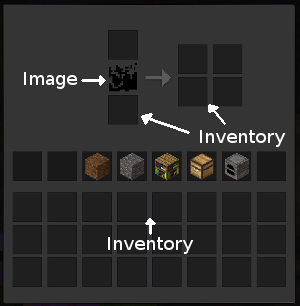
\includegraphics[width=5cm,height=\textheight,keepaspectratio,alt={Formspec eines Ofens mit Beschriftung der Elemente}]{bilder/formspec_example.png}
\caption{Formspec eines Ofens mit Beschriftung der Elemente}
\end{figure}

Musst du keine Eingaben vom Spieler entgegennehmen, sondern ihm nur
Informationen anzeigen, solltest du statt eines Formulars lieber
HUD-Elemente~(Kapitel~\ref{ch:players/hud}) verwenden. Unerwartet
aufgehende Fenster stören nämlich meist das Spiel.

\section{Echte oder alte Koordinaten}\label{echte-oder-alte-koordinaten}

In älteren Versionen von Luanti waren Formspecs uneinheitlich. Elemente
wurden auf unerwartet unterschiedliche Weise positioniert; es war schwer
vorherzusagen, wo sie landen, und sie aneinander auszurichten. Luanti
5.1.0 führte daher \emph{echte Koordinaten} (\emph{real coordinates})
ein, ein einheitliches Koordinatensystem. Echte Koordinaten sind sehr zu
empfehlen, deshalb verwendet dieses Kapitel ausschließlich sie.

Ab \texttt{formspec\_\allowbreak{}version} 2 sind echte Koordinaten
eingeschaltet.

\section{Aufbau einer Formspec}\label{aufbau-einer-formspec}

\subsection{Elemente}\label{elemente}

Formspec ist eine domänenspezifische Sprache mit einem ungewöhnlichen
Format. Sie besteht aus Elementen dieser Form:

\begin{Shaded}
\begin{Highlighting}[]
\NormalTok{typ[param1;param2]}
\end{Highlighting}
\end{Shaded}

Zuerst steht der Elementtyp, dann folgen die Parameter in eckigen
Klammern. Mehrere Elemente können direkt aneinandergehängt oder auf
mehrere Zeilen verteilt werden:

\begin{Shaded}
\begin{Highlighting}[]
\NormalTok{foo[param1]bar[param1]}
\NormalTok{bo[param1]}
\end{Highlighting}
\end{Shaded}

Elemente sind zum Beispiel Textfelder oder Schaltflächen, können aber
auch Metadaten\index{metadaten@Metadaten} wie Größe oder Hintergrund
sein. Eine Liste aller Elemente findest du in der
Lua-API-Referenz\footnote{\url{https://api.luanti.org/formspec/}}.

\subsection{Kopf}\label{kopf}

Der Kopf einer Formspec enthält Angaben, die zuerst stehen müssen: die
Größe der Formspec, ihre Position, den Anker und ob das spielweite Theme
angewendet werden soll.

Die Elemente im Kopf müssen in einer bestimmten Reihenfolge stehen,
sonst gibt es einen Fehler. Diese Reihenfolge ist die im vorigen Absatz
genannte; sie ist, wie immer, auch in der Lua-API-Referenz dokumentiert.

Die Größe wird in Formspec-Feldern angegeben, einer Maßeinheit von
ungefähr 64 Pixeln, die aber je nach Bildschirmdichte und
Skalierungseinstellungen des Clients schwankt. Hier eine Formspec der
Größe \texttt{2,2}:

\begin{Shaded}
\begin{Highlighting}[]
\NormalTok{formspec\_version[4]}
\NormalTok{size[2,2]}
\end{Highlighting}
\end{Shaded}

Beachte, dass wir die Sprachversion der Formspec ausdrücklich angegeben
haben. Ohne sie wird das alte System verwendet, und du kannst weder die
einheitliche Positionierung noch andere neue Funktionen nutzen.

Mit \texttt{position} und \texttt{anchor} platzierst du die Formspec auf
dem Bildschirm. \texttt{position} legt fest, wo auf dem Bildschirm die
Formspec erscheint; Standard ist die Mitte
(\texttt{0.\allowbreak{}5,0.\allowbreak{}5}). \texttt{anchor} legt fest,
welcher Punkt der Formspec an dieser Position liegt; so kannst du sie am
Bildschirmrand ausrichten. Am linken Rand platzierst du die Formspec so:

\begin{Shaded}
\begin{Highlighting}[]
\NormalTok{formspec\_version[4]}
\NormalTok{size[2,2]}
\NormalTok{position[0,0.5]}
\NormalTok{anchor[0,0.5]}
\end{Highlighting}
\end{Shaded}

Damit liegt der Anker in der Mitte des linken Rands der Formspec, und
dieser Anker wird an den linken Bildschirmrand gesetzt.

\section{Ein Ratespiel}\label{ein-ratespiel}

Am besten lernt man, indem man etwas baut. Bauen wir also ein Ratespiel.
Das Prinzip ist einfach: Der Mod denkt sich eine Zahl aus, und der
Spieler rät. Der Mod sagt dann, ob der Tipp zu hoch oder zu niedrig war.

\begin{figure}
\centering
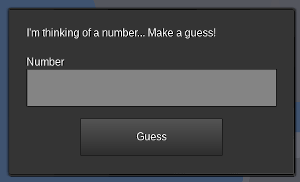
\includegraphics[width=5cm,height=\textheight,keepaspectratio,alt={Die Formspec des Ratespiels}]{bilder/formspec_guessing.png}
\caption{Die Formspec des Ratespiels}
\end{figure}

Zuerst schreiben wir eine Funktion, die den Formspec-Code erzeugt. Das
ist gute Praxis, weil sich der Code so leichter an anderer Stelle
wiederverwenden lässt.

\begin{Shaded}
\begin{Highlighting}[]
\VariableTok{guessing} \OperatorTok{=} \OperatorTok{\{\}}

\KeywordTok{function} \VariableTok{guessing}\OperatorTok{.}\NormalTok{get\_formspec}\OperatorTok{(}\VariableTok{name}\OperatorTok{)}
    \CommentTok{{-}{-} }\AlertTok{TODO}\CommentTok{: anzeigen, ob der Tipp zu hoch/niedrig war}
    \KeywordTok{local} \VariableTok{text} \OperatorTok{=} \StringTok{"Ich denke an eine Zahl ... Rate mal!"}

    \KeywordTok{local} \VariableTok{formspec} \OperatorTok{=} \OperatorTok{\{}
        \StringTok{"formspec\_version[4]"}\OperatorTok{,}
        \StringTok{"size[6,3.476]"}\OperatorTok{,}
        \StringTok{"label[0.375,0.5;"}\OperatorTok{,}
        \VariableTok{core}\OperatorTok{.}\NormalTok{formspec\_escape}\OperatorTok{(}\VariableTok{text}\OperatorTok{),}
        \StringTok{"]"}\OperatorTok{,}
        \StringTok{"field[0.375,1.25;5.25,0.8;number;Zahl;]"}\OperatorTok{,}
        \StringTok{"button[1.5,2.3;3,0.8;guess;Raten]"}\OperatorTok{,}
    \OperatorTok{\}}

    \CommentTok{{-}{-} table.concat ist schneller als Verkettung mit \textasciigrave{}..\textasciigrave{}}
    \ControlFlowTok{return} \FunctionTok{table.concat}\OperatorTok{(}\VariableTok{formspec}\OperatorTok{,} \StringTok{""}\OperatorTok{)}
\KeywordTok{end}
\end{Highlighting}
\end{Shaded}

Hier platzieren wir ein Eingabefeld, eine Beschriftung und eine
Schaltfläche. In das Feld kann man Text eingeben, die Schaltfläche
schickt das Formular ab. Die Elemente sind sorgfältig positioniert, um
Innenabstand und Zwischenraum zu erzeugen; das wird gleich erklärt.

Als Nächstes soll der Spieler die Formspec öffnen können. Der übliche
Weg dafür ist \texttt{show\_\allowbreak{}formspec}:

\begin{Shaded}
\begin{Highlighting}[]
\KeywordTok{function} \VariableTok{guessing}\OperatorTok{.}\NormalTok{show\_to}\OperatorTok{(}\VariableTok{name}\OperatorTok{)}
    \VariableTok{core}\OperatorTok{.}\NormalTok{show\_formspec}\OperatorTok{(}
        \VariableTok{name}\OperatorTok{,}
        \StringTok{"guessing:game"}\OperatorTok{,}
        \VariableTok{guessing}\OperatorTok{.}\NormalTok{get\_formspec}\OperatorTok{(}\VariableTok{name}\OperatorTok{)}
    \OperatorTok{)}
\KeywordTok{end}

\VariableTok{core}\OperatorTok{.}\NormalTok{register\_chatcommand}\OperatorTok{(}\StringTok{"game"}\OperatorTok{,} \OperatorTok{\{}
    \VariableTok{func} \OperatorTok{=} \KeywordTok{function}\OperatorTok{(}\VariableTok{name}\OperatorTok{)}
        \VariableTok{guessing}\OperatorTok{.}\NormalTok{show\_to}\OperatorTok{(}\VariableTok{name}\OperatorTok{)}
    \KeywordTok{end}\OperatorTok{,}
\OperatorTok{\})}
\end{Highlighting}
\end{Shaded}

\texttt{show\_\allowbreak{}formspec} erwartet einen Spielernamen, den
Namen der Formspec und die Formspec selbst. Der Name der Formspec sollte
ein gültiger Itemname sein, also im Format \texttt{modname:itemname}.

\subsection{Innenabstand und
Zwischenraum}\label{innenabstand-und-zwischenraum}

\begin{figure}
\centering
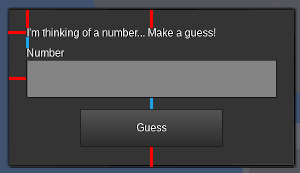
\includegraphics[width=5cm,height=\textheight,keepaspectratio,alt={Innenabstand (rot) und Zwischenraum (blau)}]{bilder/formspec_padding_spacing.png}
\caption{Innenabstand (rot) und Zwischenraum (blau)}
\end{figure}

Der Innenabstand (\emph{padding}, rot) ist der Abstand zwischen dem Rand
der Formspec und ihrem Inhalt oder zwischen Elementen, die nicht
zusammengehören. Der Zwischenraum (\emph{spacing}, blau) ist der Abstand
zwischen zusammengehörenden Elementen.

Üblich sind ein Innenabstand von \texttt{0.\allowbreak{}375} und ein
Zwischenraum von \texttt{0.\allowbreak{}25}.

\subsection{Eingaben empfangen}\label{eingaben-empfangen}

Beim Aufruf von \texttt{show\_\allowbreak{}formspec} wird die Formspec
zum Client geschickt und dort angezeigt. Nützlich wird sie aber erst,
wenn Informationen vom Client zum Server zurückkommen. Dieser Vorgang
heißt \emph{Formspec field submission}; bei
\texttt{show\_\allowbreak{}formspec} empfängst du die Eingaben mit einem
globalen Callback:\index{callback@Callback}

\begin{Shaded}
\begin{Highlighting}[]
\VariableTok{core}\OperatorTok{.}\NormalTok{register\_on\_player\_receive\_fields}\OperatorTok{(}
    \KeywordTok{function}\OperatorTok{(}\VariableTok{player}\OperatorTok{,} \VariableTok{formname}\OperatorTok{,} \VariableTok{fields}\OperatorTok{)}
        \ControlFlowTok{if} \VariableTok{formname} \OperatorTok{\textasciitilde{}=} \StringTok{"guessing:game"} \ControlFlowTok{then}
            \ControlFlowTok{return}
        \ControlFlowTok{end}

        \ControlFlowTok{if} \VariableTok{fields}\OperatorTok{.}\VariableTok{guess} \ControlFlowTok{then}
            \KeywordTok{local} \VariableTok{pname} \OperatorTok{=} \VariableTok{player}\OperatorTok{:}\NormalTok{get\_player\_name}\OperatorTok{()}
            \VariableTok{core}\OperatorTok{.}\NormalTok{chat\_send\_all}\OperatorTok{(}
                \VariableTok{pname}
                    \OperatorTok{..} \StringTok{" hat "}
                    \OperatorTok{..} \VariableTok{fields}\OperatorTok{.}\VariableTok{number}
                    \OperatorTok{..} \StringTok{" geraten"}
            \OperatorTok{)}
        \ControlFlowTok{end}
    \KeywordTok{end}
\OperatorTok{)}
\end{Highlighting}
\end{Shaded}

Die an
\texttt{core.\allowbreak{}register\_\allowbreak{}on\_\allowbreak{}player\_\allowbreak{}receive\_\allowbreak{}fields}\index{core@\texttt{core}!register_on_player_receive_fields@\texttt{core.\allowbreak{}register\_\allowbreak{}on\_\allowbreak{}player\_\allowbreak{}receive\_\allowbreak{}fields}}
übergebene Funktion wird jedes Mal aufgerufen, wenn ein Spieler ein
Formular abschickt. Die meisten Callbacks müssen den übergebenen
Formularnamen prüfen und abbrechen, wenn es nicht das richtige Formular
ist; manche Callbacks arbeiten aber auch mit mehreren oder allen
Formularen.

Der Parameter \texttt{fields} ist eine Tabelle mit den Werten, die der
Spieler abgeschickt hat, indiziert mit Strings. Benannte Elemente
erscheinen je nach Ereignis unter ihrem eigenen Namen. Manche Elemente,
etwa Schaltflächen, werden nur übermittelt, wenn sie das Ereignis
ausgelöst haben; andere, etwa Eingabefelder, sind immer dabei.

\begin{hinweis}{Bösartige Clients können jederzeit alles schicken}

Vertraue niemals den abgeschickten Daten einer Formspec. Ein bösartiger
Client kann jederzeit alles Mögliche schicken -- selbst wenn du ihm die
Formspec nie angezeigt hast. Prüfe also
Privilegien\index{privileg@Privileg} und stelle sicher, dass der Spieler
die Aktion wirklich ausführen darf.

\end{hinweis}

Die Formspec wird jetzt also zum Client geschickt, und der Client
schickt Informationen zurück. Als Nächstes müssen wir die Zielzahl
irgendwie erzeugen und uns merken und die Formspec abhängig von den
Tipps aktualisieren. Dafür gibt es das Konzept der \emph{Kontexte}.

\subsection{Kontexte}\label{kontexte}

Oft soll
\texttt{core.\allowbreak{}show\_\allowbreak{}formspec}\index{core@\texttt{core}!show_formspec@\texttt{core.\allowbreak{}show\_\allowbreak{}formspec}}
dem Callback Informationen mitgeben, die der Client nicht sehen soll --
etwa, mit welchen Argumenten ein Chatbefehl\index{chatbefehl@Chatbefehl}
aufgerufen wurde oder worum es in dem Dialog geht. Hier ist es die
Zielzahl, die wir uns merken müssen.

Ein Kontext ist eine Tabelle je Spieler, in der Informationen
gespeichert werden. Die Kontexte aller Spieler, die gerade online sind,
liegen in einer lokalen Variablen der Datei:

\begin{Shaded}
\begin{Highlighting}[]
\KeywordTok{local} \VariableTok{\_contexts} \OperatorTok{=} \OperatorTok{\{\}}
\KeywordTok{local} \KeywordTok{function}\NormalTok{ get\_context}\OperatorTok{(}\VariableTok{name}\OperatorTok{)}
    \KeywordTok{local} \VariableTok{context} \OperatorTok{=} \VariableTok{\_contexts}\OperatorTok{[}\VariableTok{name}\OperatorTok{]} \KeywordTok{or} \OperatorTok{\{\}}
    \VariableTok{\_contexts}\OperatorTok{[}\VariableTok{name}\OperatorTok{]} \OperatorTok{=} \VariableTok{context}
    \ControlFlowTok{return} \VariableTok{context}
\KeywordTok{end}

\VariableTok{core}\OperatorTok{.}\NormalTok{register\_on\_leaveplayer}\OperatorTok{(}\KeywordTok{function}\OperatorTok{(}\VariableTok{player}\OperatorTok{)}
    \VariableTok{\_contexts}\OperatorTok{[}\VariableTok{player}\OperatorTok{:}\NormalTok{get\_player\_name}\OperatorTok{()]} \OperatorTok{=} \KeywordTok{nil}
\KeywordTok{end}\OperatorTok{)}
\end{Highlighting}
\end{Shaded}

Nun ändern wir den Code zum Anzeigen so, dass er den Kontext
aktualisiert, bevor er die Formspec anzeigt:

\begin{Shaded}
\begin{Highlighting}[]
\KeywordTok{function} \VariableTok{guessing}\OperatorTok{.}\NormalTok{show\_to}\OperatorTok{(}\VariableTok{name}\OperatorTok{)}
    \KeywordTok{local} \VariableTok{context} \OperatorTok{=}\NormalTok{ get\_context}\OperatorTok{(}\VariableTok{name}\OperatorTok{)}
    \VariableTok{context}\OperatorTok{.}\VariableTok{target} \OperatorTok{=} \VariableTok{context}\OperatorTok{.}\VariableTok{target} \KeywordTok{or} \FunctionTok{math.random}\OperatorTok{(}\DecValTok{1}\OperatorTok{,} \DecValTok{10}\OperatorTok{)}

    \KeywordTok{local} \VariableTok{fs} \OperatorTok{=} \VariableTok{guessing}\OperatorTok{.}\NormalTok{get\_formspec}\OperatorTok{(}\VariableTok{name}\OperatorTok{,} \VariableTok{context}\OperatorTok{)}
    \VariableTok{core}\OperatorTok{.}\NormalTok{show\_formspec}\OperatorTok{(}\VariableTok{name}\OperatorTok{,} \StringTok{"guessing:game"}\OperatorTok{,} \VariableTok{fs}\OperatorTok{)}
\KeywordTok{end}
\end{Highlighting}
\end{Shaded}

Auch der Code, der die Formspec erzeugt, muss den Kontext verwenden:

\begin{Shaded}
\begin{Highlighting}[]
\KeywordTok{function} \VariableTok{guessing}\OperatorTok{.}\NormalTok{get\_formspec}\OperatorTok{(}\VariableTok{name}\OperatorTok{,} \VariableTok{context}\OperatorTok{)}
    \KeywordTok{local} \VariableTok{text}
    \ControlFlowTok{if} \KeywordTok{not} \VariableTok{context}\OperatorTok{.}\VariableTok{guess} \ControlFlowTok{then}
        \VariableTok{text} \OperatorTok{=} \StringTok{"Ich denke an eine Zahl ... Rate mal!"}
    \ControlFlowTok{elseif} \VariableTok{context}\OperatorTok{.}\VariableTok{guess} \OperatorTok{==} \VariableTok{context}\OperatorTok{.}\VariableTok{target} \ControlFlowTok{then}
        \VariableTok{text} \OperatorTok{=} \StringTok{"Hurra, richtig geraten!"}
    \ControlFlowTok{elseif} \VariableTok{context}\OperatorTok{.}\VariableTok{guess} \OperatorTok{\textgreater{}} \VariableTok{context}\OperatorTok{.}\VariableTok{target} \ControlFlowTok{then}
        \VariableTok{text} \OperatorTok{=} \StringTok{"Zu hoch!"}
    \ControlFlowTok{else}
        \VariableTok{text} \OperatorTok{=} \StringTok{"Zu niedrig!"}
    \ControlFlowTok{end}

    \CommentTok{{-}{-} … weiter wie oben}
\KeywordTok{end}
\end{Highlighting}
\end{Shaded}

Es ist gute Praxis, dass \texttt{get\_\allowbreak{}formspec} den Kontext
nur liest und nie verändert. Das hält die Funktion einfacher und
leichter testbar.

Zum Schluss muss der Handler den Kontext mit dem Tipp aktualisieren:

\begin{Shaded}
\begin{Highlighting}[]
\ControlFlowTok{if} \VariableTok{fields}\OperatorTok{.}\VariableTok{guess} \ControlFlowTok{then}
    \KeywordTok{local} \VariableTok{name} \OperatorTok{=} \VariableTok{player}\OperatorTok{:}\NormalTok{get\_player\_name}\OperatorTok{()}
    \KeywordTok{local} \VariableTok{context} \OperatorTok{=}\NormalTok{ get\_context}\OperatorTok{(}\VariableTok{name}\OperatorTok{)}
    \VariableTok{context}\OperatorTok{.}\VariableTok{guess} \OperatorTok{=} \FunctionTok{tonumber}\OperatorTok{(}\VariableTok{fields}\OperatorTok{.}\VariableTok{number}\OperatorTok{)}
    \VariableTok{guessing}\OperatorTok{.}\NormalTok{show\_to}\OperatorTok{(}\VariableTok{name}\OperatorTok{)}
\ControlFlowTok{end}
\end{Highlighting}
\end{Shaded}

\section{Wege zur Formspec}\label{wege-zur-formspec}

Eine Formspec kann auf drei Wegen zum Client gelangen:

\begin{itemize}
\tightlist
\item
  show\_formspec: der oben verwendete Weg; die Eingaben empfängt
  \texttt{register\_\allowbreak{}on\_\allowbreak{}player\_\allowbreak{}receive\_\allowbreak{}fields}.
\item
  Formspecs in Node-Metadaten: Der Node hat eine Formspec in seinen
  Metadaten, und der Client zeigt sie \emph{sofort} an, wenn der Spieler
  rechts klickt. Die Eingaben empfängt die Methode
  \texttt{on\_\allowbreak{}receive\_\allowbreak{}fields}\index{callback@Callback!on_receive_fields@\texttt{on\_\allowbreak{}receive\_\allowbreak{}fields}}
  in der Node-Definition.
\item
  Formspecs im Spielerinventar: Die Formspec wird irgendwann zum Client
  geschickt und sofort angezeigt, wenn der Spieler \texttt{i} drückt.
  Die Eingaben empfängt
  \texttt{register\_\allowbreak{}on\_\allowbreak{}player\_\allowbreak{}receive\_\allowbreak{}fields}.
\end{itemize}

\subsection{Formspecs in
Node-Metadaten}\label{formspecs-in-node-metadaten}

\texttt{core.\allowbreak{}show\_\allowbreak{}formspec} ist nicht der
einzige Weg, eine Formspec anzuzeigen; du kannst Formspecs auch in die
Metadaten eines Nodes~(Kapitel~\ref{ch:map/storage}) schreiben. Truhen
machen das zum Beispiel, damit sie schneller aufgehen -- man muss nicht
warten, bis der Server die Formspec der Truhe schickt.

\begin{Shaded}
\begin{Highlighting}[]
\VariableTok{core}\OperatorTok{.}\NormalTok{register\_node}\OperatorTok{(}\StringTok{"mymod:rightclick"}\OperatorTok{,} \OperatorTok{\{}
    \VariableTok{description} \OperatorTok{=} \StringTok{"Klick mich mit rechts!"}\OperatorTok{,}
    \VariableTok{tiles} \OperatorTok{=} \OperatorTok{\{} \StringTok{"mymod\_rightclick.png"} \OperatorTok{\},}
    \VariableTok{groups} \OperatorTok{=} \OperatorTok{\{} \VariableTok{cracky} \OperatorTok{=} \DecValTok{1} \OperatorTok{\},}
    \VariableTok{after\_place\_node} \OperatorTok{=} \KeywordTok{function}\OperatorTok{(}\VariableTok{pos}\OperatorTok{,} \VariableTok{placer}\OperatorTok{)}
        \CommentTok{{-}{-} Läuft, wenn der Node platziert wird, und setzt}
        \CommentTok{{-}{-} die Formspec in den Metadaten des Nodes.}
        \KeywordTok{local} \VariableTok{meta} \OperatorTok{=} \VariableTok{core}\OperatorTok{.}\NormalTok{get\_meta}\OperatorTok{(}\VariableTok{pos}\OperatorTok{)}
        \VariableTok{meta}\OperatorTok{:}\NormalTok{set\_string}\OperatorTok{(}
            \StringTok{"formspec"}\OperatorTok{,}
            \StringTok{"formspec\_version[4]"}
                \OperatorTok{..} \StringTok{"size[5,5]"}
                \OperatorTok{..} \StringTok{"label[1,1;Erscheint beim Rechtsklick]"}
                \OperatorTok{..} \StringTok{"field[1,2;2,1;x;x;]"}
        \OperatorTok{)}
    \KeywordTok{end}\OperatorTok{,}
    \VariableTok{on\_receive\_fields} \OperatorTok{=} \KeywordTok{function}\OperatorTok{(}
        \VariableTok{pos}\OperatorTok{,}
        \VariableTok{formname}\OperatorTok{,}
        \VariableTok{fields}\OperatorTok{,}
        \VariableTok{player}
    \OperatorTok{)}
        \ControlFlowTok{if} \VariableTok{fields}\OperatorTok{.}\VariableTok{quit} \ControlFlowTok{then}
            \ControlFlowTok{return}
        \ControlFlowTok{end}

        \FunctionTok{print}\OperatorTok{(}\VariableTok{fields}\OperatorTok{.}\VariableTok{x}\OperatorTok{)}
    \KeywordTok{end}\OperatorTok{,}
\OperatorTok{\})}
\end{Highlighting}
\end{Shaded}

So gesetzte Formspecs lösen nicht denselben Callback aus. Um Eingaben
aus Formspecs in Metadaten zu empfangen, musst du bei der Registrierung
des Nodes einen Eintrag
\texttt{on\_\allowbreak{}receive\_\allowbreak{}fields} angeben.

Dieser Callback wird auch ausgelöst, wenn du in einem Feld die
Eingabetaste drückst, was mit
\texttt{core.\allowbreak{}show\_\allowbreak{}formspec} nicht möglich
ist. Dafür lässt sich diese Art von Formular nur durch einen Rechtsklick
auf den Node öffnen, nicht per Programmcode.

\subsection{Formspecs im
Spielerinventar}\label{formspecs-im-spielerinventar}

Die Formspec des Spielerinventars erscheint, wenn der Spieler \texttt{i}
drückt. Ihre Ereignisse empfängst du mit dem globalen Callback; der
Formularname ist dabei \texttt{\textquotedbl{}\textquotedbl{}}.

Es gibt verschiedene Mods, mit denen mehrere Mods gemeinsam das
Spielerinventar anpassen können. Minetest Game verwendet
SFINV\footnote{\url{https://github.com/rubenwardy/sfinv/blob/master/Tutorial.md}}.

\subsection{Jetzt bist du dran}\label{jetzt-bist-du-dran}

\begin{itemize}
\tightlist
\item
  Erweitere das Ratespiel so, dass es sich für jeden Spieler die
  Bestleistung merkt, also mit wie wenigen Tipps er die Zahl erraten
  hat.
\item
  Erstelle einen Node „Briefkasten``, in dem Spieler über eine Formspec
  Nachrichten hinterlassen können. Der Node soll den Namen des
  Platzierenden als \texttt{owner} in den Metadaten speichern und mit
  \texttt{show\_\allowbreak{}formspec} unterschiedlichen Spielern
  unterschiedliche Formspecs zeigen.
\end{itemize}

\chapter{HUD}
\label{ch:players/hud}

Mit HUD-Elementen (\emph{Heads-up-Display}) zeigst du Text, Bilder und
andere grafische Elemente an.

Das HUD\index{hud@HUD} nimmt keine Eingaben entgegen; dafür verwendest
du eine
Formspec\index{formspec@Formspec}~(Kapitel~\ref{ch:players/formspecs}).

\begin{hinweis}{type statt hud\_elem\_type}

Seit Luanti 5.9 heißt die Eigenschaft für den Elementtyp \texttt{type}.
Der alte Name \texttt{hud\_\allowbreak{}elem\_\allowbreak{}type}
funktioniert noch, gilt aber als veraltet. Dieses Kapitel verwendet
durchgehend \texttt{type}.

\end{hinweis}

\section{Positionierung}\label{positionierung}

\subsection{Position und Versatz}\label{position-und-versatz}

\begin{figure}
\centering
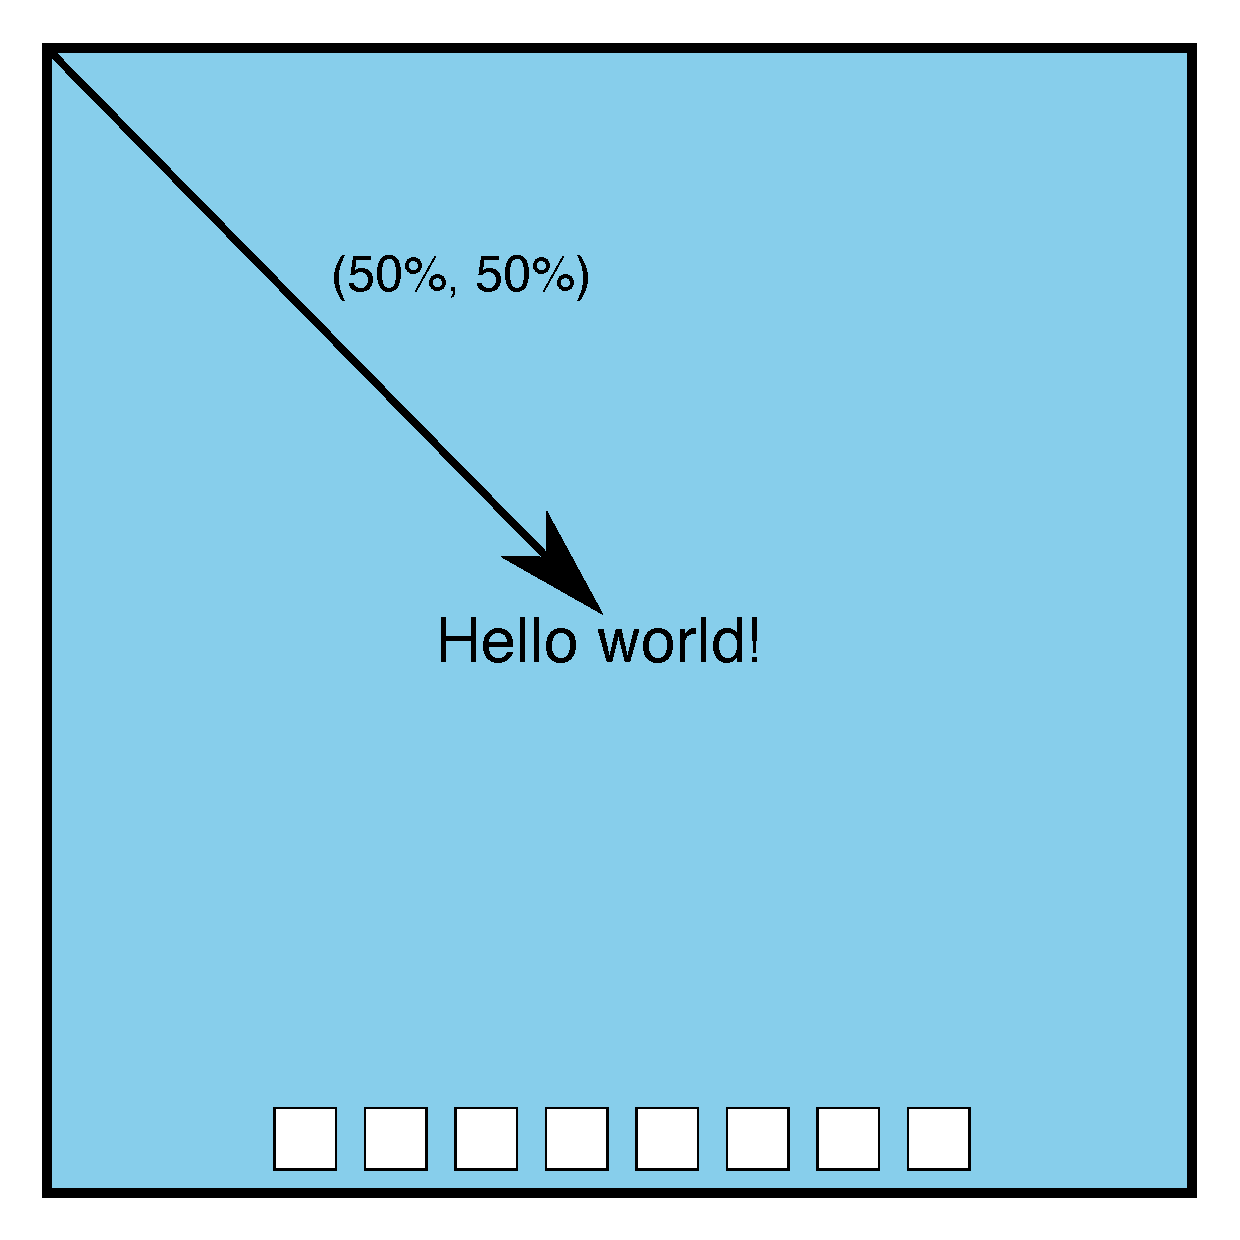
\includegraphics[width=6cm,height=\textheight,keepaspectratio,alt={Ein zentriertes Textelement}]{bilder/hud_diagram_center.pdf}
\caption{Ein zentriertes Textelement}
\end{figure}

Bildschirme gibt es in vielen Größen und Auflösungen, und das HUD muss
auf allen gut funktionieren.

Luanti löst das, indem die Lage eines Elements aus einer prozentualen
Position und einem Versatz (\emph{offset}) bestimmt wird. Die
prozentuale Position bezieht sich auf die Bildschirmgröße. Um ein
Element in der Bildschirmmitte zu platzieren, gibst du also die halbe
Bildschirmgröße als Position an, etwa (50 \%, 50 \%), und einen Versatz
von (0, 0).

Mit dem Versatz verschiebst du das Element dann relativ zur prozentualen
Position.

\subsection{Ausrichtung}\label{ausrichtung}

Die Ausrichtung (\emph{alignment}) legt fest, wo am Element der aus
Position und Versatz berechnete Punkt liegt. Mit
\texttt{\{x = -1.\allowbreak{}0, y = 0.\allowbreak{}0\}} zeigt dieser
Punkt zum Beispiel auf den linken Rand des Elements. Das ist besonders
nützlich, um Text links, mittig oder rechts auszurichten.

\begin{figure}
\centering
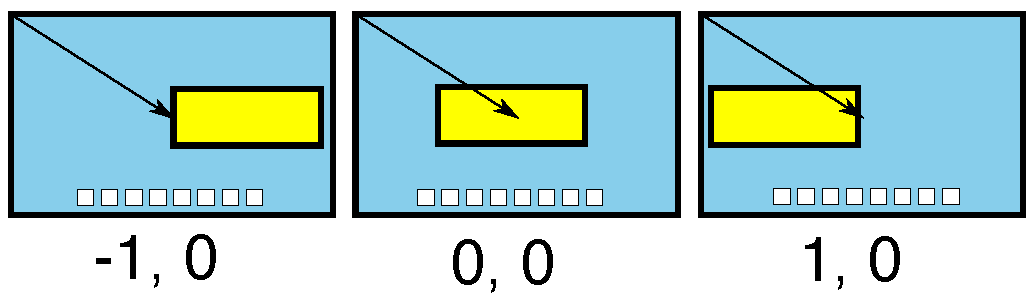
\includegraphics[width=10cm,height=\textheight,keepaspectratio,alt={Ausrichtung}]{bilder/hud_diagram_alignment.pdf}
\caption{Ausrichtung}
\end{figure}

Das Diagramm zeigt drei Fenster (blau) mit jeweils einem HUD-Element
(gelb) und unterschiedlicher Ausrichtung. Der Pfeil ist das Ergebnis aus
Position und Versatz.

\subsection{Punkteanzeige}\label{punkteanzeige}

In diesem Kapitel lernst du, eine Punkteanzeige wie diese zu
positionieren und zu aktualisieren:

\begin{figure}
\centering
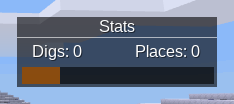
\includegraphics[width=5cm,height=\textheight,keepaspectratio,alt={So soll das HUD am Ende aussehen}]{bilder/hud_final.png}
\caption{So soll das HUD am Ende aussehen}
\end{figure}

Im Bild haben alle Elemente dieselbe prozentuale Position (100 \%, 50
\%), aber unterschiedliche Versätze. So ist das Ganze am rechten
Fensterrand verankert und bleibt beim Ändern der Fenstergröße intakt.

\section{Textelemente}\label{textelemente}

Sobald du das Spielerobjekt hast, kannst du ein HUD-Element anlegen:

\begin{Shaded}
\begin{Highlighting}[]
\KeywordTok{local} \VariableTok{player} \OperatorTok{=} \VariableTok{core}\OperatorTok{.}\NormalTok{get\_player\_by\_name}\OperatorTok{(}\StringTok{"username"}\OperatorTok{)}
\KeywordTok{local} \VariableTok{idx} \OperatorTok{=} \VariableTok{player}\OperatorTok{:}\NormalTok{hud\_add}\OperatorTok{(\{}
    \FunctionTok{type} \OperatorTok{=} \StringTok{"text"}\OperatorTok{,}
    \VariableTok{position} \OperatorTok{=} \OperatorTok{\{} \VariableTok{x} \OperatorTok{=} \DecValTok{0.5}\OperatorTok{,} \VariableTok{y} \OperatorTok{=} \DecValTok{0.5} \OperatorTok{\},}
    \VariableTok{offset} \OperatorTok{=} \OperatorTok{\{} \VariableTok{x} \OperatorTok{=} \DecValTok{0}\OperatorTok{,} \VariableTok{y} \OperatorTok{=} \DecValTok{0} \OperatorTok{\},}
    \VariableTok{text} \OperatorTok{=} \StringTok{"Hallo Welt!"}\OperatorTok{,}
    \VariableTok{alignment} \OperatorTok{=} \OperatorTok{\{} \VariableTok{x} \OperatorTok{=} \DecValTok{0}\OperatorTok{,} \VariableTok{y} \OperatorTok{=} \DecValTok{0} \OperatorTok{\},} \CommentTok{{-}{-} zentriert}
    \VariableTok{scale} \OperatorTok{=} \OperatorTok{\{} \VariableTok{x} \OperatorTok{=} \DecValTok{100}\OperatorTok{,} \VariableTok{y} \OperatorTok{=} \DecValTok{100} \OperatorTok{\},} \CommentTok{{-}{-} siehe unten}
\OperatorTok{\})}
\end{Highlighting}
\end{Shaded}

\texttt{hud\_\allowbreak{}add} gibt eine Element-ID zurück, mit der du
das HUD-Element später ändern oder entfernen kannst.

\subsection{Parameter}\label{parameter}

Den Elementtyp gibst du mit der Eigenschaft \texttt{type} in der
Definitionstabelle an. Die Bedeutung der übrigen Eigenschaften hängt vom
Typ ab.

\texttt{scale} ist der maximale Bereich für den Text; Text außerhalb
wird abgeschnitten, z.~B. \texttt{\{x=100, y=100\}}.

\texttt{number} ist die Textfarbe als Hexadezimalzahl, z.~B.
\texttt{0xFF0000}.

\subsection{Unser Beispiel}\label{unser-beispiel}

Platzieren wir nun alle Texte unserer Punkteanzeige:

\begin{Shaded}
\begin{Highlighting}[]
\CommentTok{{-}{-} Zähler aus dem Speicher holen, Standard 0}
\KeywordTok{local} \VariableTok{meta} \OperatorTok{=} \VariableTok{player}\OperatorTok{:}\NormalTok{get\_meta}\OperatorTok{()}
\KeywordTok{local} \VariableTok{digs\_text} \OperatorTok{=} \StringTok{"Abgebaut: "} \OperatorTok{..} \VariableTok{meta}\OperatorTok{:}\NormalTok{get\_int}\OperatorTok{(}\StringTok{"score:digs"}\OperatorTok{)}
\KeywordTok{local} \VariableTok{places\_text} \OperatorTok{=} \StringTok{"Platziert: "}
    \OperatorTok{..} \VariableTok{meta}\OperatorTok{:}\NormalTok{get\_int}\OperatorTok{(}\StringTok{"score:places"}\OperatorTok{)}

\VariableTok{player}\OperatorTok{:}\NormalTok{hud\_add}\OperatorTok{(\{}
    \FunctionTok{type} \OperatorTok{=} \StringTok{"text"}\OperatorTok{,}
    \VariableTok{position} \OperatorTok{=} \OperatorTok{\{} \VariableTok{x} \OperatorTok{=} \DecValTok{1}\OperatorTok{,} \VariableTok{y} \OperatorTok{=} \DecValTok{0.5} \OperatorTok{\},}
    \VariableTok{offset} \OperatorTok{=} \OperatorTok{\{} \VariableTok{x} \OperatorTok{=} \OperatorTok{{-}}\DecValTok{120}\OperatorTok{,} \VariableTok{y} \OperatorTok{=} \OperatorTok{{-}}\DecValTok{25} \OperatorTok{\},}
    \VariableTok{text} \OperatorTok{=} \StringTok{"Statistik"}\OperatorTok{,}
    \VariableTok{alignment} \OperatorTok{=} \OperatorTok{\{} \VariableTok{x} \OperatorTok{=} \DecValTok{0}\OperatorTok{,} \VariableTok{y} \OperatorTok{=} \DecValTok{0} \OperatorTok{\},}
    \VariableTok{scale} \OperatorTok{=} \OperatorTok{\{} \VariableTok{x} \OperatorTok{=} \DecValTok{100}\OperatorTok{,} \VariableTok{y} \OperatorTok{=} \DecValTok{30} \OperatorTok{\},}
    \VariableTok{number} \OperatorTok{=} \DecValTok{0xFFFFFF}\OperatorTok{,}
\OperatorTok{\})}

\VariableTok{player}\OperatorTok{:}\NormalTok{hud\_add}\OperatorTok{(\{}
    \FunctionTok{type} \OperatorTok{=} \StringTok{"text"}\OperatorTok{,}
    \VariableTok{position} \OperatorTok{=} \OperatorTok{\{} \VariableTok{x} \OperatorTok{=} \DecValTok{1}\OperatorTok{,} \VariableTok{y} \OperatorTok{=} \DecValTok{0.5} \OperatorTok{\},}
    \VariableTok{offset} \OperatorTok{=} \OperatorTok{\{} \VariableTok{x} \OperatorTok{=} \OperatorTok{{-}}\DecValTok{180}\OperatorTok{,} \VariableTok{y} \OperatorTok{=} \DecValTok{0} \OperatorTok{\},}
    \VariableTok{text} \OperatorTok{=} \VariableTok{digs\_text}\OperatorTok{,}
    \VariableTok{alignment} \OperatorTok{=} \OperatorTok{\{} \VariableTok{x} \OperatorTok{=} \OperatorTok{{-}}\DecValTok{1}\OperatorTok{,} \VariableTok{y} \OperatorTok{=} \DecValTok{0} \OperatorTok{\},}
    \VariableTok{scale} \OperatorTok{=} \OperatorTok{\{} \VariableTok{x} \OperatorTok{=} \DecValTok{50}\OperatorTok{,} \VariableTok{y} \OperatorTok{=} \DecValTok{10} \OperatorTok{\},}
    \VariableTok{number} \OperatorTok{=} \DecValTok{0xFFFFFF}\OperatorTok{,}
\OperatorTok{\})}

\VariableTok{player}\OperatorTok{:}\NormalTok{hud\_add}\OperatorTok{(\{}
    \FunctionTok{type} \OperatorTok{=} \StringTok{"text"}\OperatorTok{,}
    \VariableTok{position} \OperatorTok{=} \OperatorTok{\{} \VariableTok{x} \OperatorTok{=} \DecValTok{1}\OperatorTok{,} \VariableTok{y} \OperatorTok{=} \DecValTok{0.5} \OperatorTok{\},}
    \VariableTok{offset} \OperatorTok{=} \OperatorTok{\{} \VariableTok{x} \OperatorTok{=} \OperatorTok{{-}}\DecValTok{70}\OperatorTok{,} \VariableTok{y} \OperatorTok{=} \DecValTok{0} \OperatorTok{\},}
    \VariableTok{text} \OperatorTok{=} \VariableTok{places\_text}\OperatorTok{,}
    \VariableTok{alignment} \OperatorTok{=} \OperatorTok{\{} \VariableTok{x} \OperatorTok{=} \OperatorTok{{-}}\DecValTok{1}\OperatorTok{,} \VariableTok{y} \OperatorTok{=} \DecValTok{0} \OperatorTok{\},}
    \VariableTok{scale} \OperatorTok{=} \OperatorTok{\{} \VariableTok{x} \OperatorTok{=} \DecValTok{50}\OperatorTok{,} \VariableTok{y} \OperatorTok{=} \DecValTok{10} \OperatorTok{\},}
    \VariableTok{number} \OperatorTok{=} \DecValTok{0xFFFFFF}\OperatorTok{,}
\OperatorTok{\})}
\end{Highlighting}
\end{Shaded}

Das ergibt Folgendes:

\begin{figure}
\centering
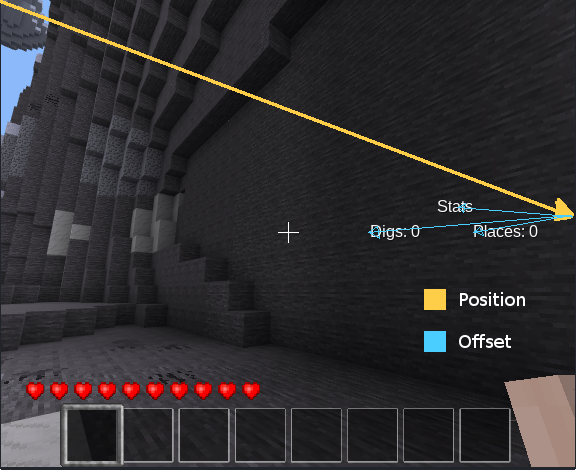
\includegraphics[width=6cm,height=\textheight,keepaspectratio,alt={Die Textelemente der Punkteanzeige}]{bilder/hud_text.png}
\caption{Die Textelemente der Punkteanzeige}
\end{figure}

\section{Bildelemente}\label{bildelemente}

Bildelemente legst du ganz ähnlich an wie Textelemente:

\begin{Shaded}
\begin{Highlighting}[]
\VariableTok{player}\OperatorTok{:}\NormalTok{hud\_add}\OperatorTok{(\{}
    \FunctionTok{type} \OperatorTok{=} \StringTok{"image"}\OperatorTok{,}
    \VariableTok{position} \OperatorTok{=} \OperatorTok{\{} \VariableTok{x} \OperatorTok{=} \DecValTok{1}\OperatorTok{,} \VariableTok{y} \OperatorTok{=} \DecValTok{0.5} \OperatorTok{\},}
    \VariableTok{offset} \OperatorTok{=} \OperatorTok{\{} \VariableTok{x} \OperatorTok{=} \OperatorTok{{-}}\DecValTok{220}\OperatorTok{,} \VariableTok{y} \OperatorTok{=} \DecValTok{0} \OperatorTok{\},}
    \VariableTok{text} \OperatorTok{=} \StringTok{"score\_background.png"}\OperatorTok{,}
    \VariableTok{scale} \OperatorTok{=} \OperatorTok{\{} \VariableTok{x} \OperatorTok{=} \DecValTok{1}\OperatorTok{,} \VariableTok{y} \OperatorTok{=} \DecValTok{1} \OperatorTok{\},}
    \VariableTok{alignment} \OperatorTok{=} \OperatorTok{\{} \VariableTok{x} \OperatorTok{=} \DecValTok{1}\OperatorTok{,} \VariableTok{y} \OperatorTok{=} \DecValTok{0} \OperatorTok{\},}
\OperatorTok{\})}
\end{Highlighting}
\end{Shaded}

Jetzt sieht es so aus:

\begin{figure}
\centering
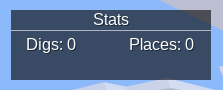
\includegraphics[width=5cm,height=\textheight,keepaspectratio,alt={Die Punkteanzeige mit Hintergrundbild}]{bilder/hud_background_img.png}
\caption{Die Punkteanzeige mit Hintergrundbild}
\end{figure}

\subsection{Parameter}\label{parameter-1}

Im Feld \texttt{text} steht der Name des Bildes.

Ist eine Koordinate von \texttt{scale} positiv, ist sie ein
Skalierungsfaktor: 1 ist die Originalgröße, 2 die doppelte Größe und so
weiter. Ist sie negativ, ist sie ein Prozentwert der Bildschirmgröße;
\texttt{x=-100} bedeutet zum Beispiel 100 \% der Breite.

\subsection{Skalierung}\label{skalierung}

Als Beispiel für die Skalierung bauen wir den Fortschrittsbalken der
Punkteanzeige:

\begin{Shaded}
\begin{Highlighting}[]
\KeywordTok{local} \VariableTok{percent} \OperatorTok{=} \FunctionTok{tonumber}\OperatorTok{(}\VariableTok{meta}\OperatorTok{:}\NormalTok{get}\OperatorTok{(}\StringTok{"score:score"}\OperatorTok{)} \KeywordTok{or} \DecValTok{0.2}\OperatorTok{)}

\VariableTok{player}\OperatorTok{:}\NormalTok{hud\_add}\OperatorTok{(\{}
    \FunctionTok{type} \OperatorTok{=} \StringTok{"image"}\OperatorTok{,}
    \VariableTok{position} \OperatorTok{=} \OperatorTok{\{} \VariableTok{x} \OperatorTok{=} \DecValTok{1}\OperatorTok{,} \VariableTok{y} \OperatorTok{=} \DecValTok{0.5} \OperatorTok{\},}
    \VariableTok{offset} \OperatorTok{=} \OperatorTok{\{} \VariableTok{x} \OperatorTok{=} \OperatorTok{{-}}\DecValTok{215}\OperatorTok{,} \VariableTok{y} \OperatorTok{=} \DecValTok{23} \OperatorTok{\},}
    \VariableTok{text} \OperatorTok{=} \StringTok{"score\_bar\_empty.png"}\OperatorTok{,}
    \VariableTok{scale} \OperatorTok{=} \OperatorTok{\{} \VariableTok{x} \OperatorTok{=} \DecValTok{1}\OperatorTok{,} \VariableTok{y} \OperatorTok{=} \DecValTok{1} \OperatorTok{\},}
    \VariableTok{alignment} \OperatorTok{=} \OperatorTok{\{} \VariableTok{x} \OperatorTok{=} \DecValTok{1}\OperatorTok{,} \VariableTok{y} \OperatorTok{=} \DecValTok{0} \OperatorTok{\},}
\OperatorTok{\})}

\VariableTok{player}\OperatorTok{:}\NormalTok{hud\_add}\OperatorTok{(\{}
    \FunctionTok{type} \OperatorTok{=} \StringTok{"image"}\OperatorTok{,}
    \VariableTok{position} \OperatorTok{=} \OperatorTok{\{} \VariableTok{x} \OperatorTok{=} \DecValTok{1}\OperatorTok{,} \VariableTok{y} \OperatorTok{=} \DecValTok{0.5} \OperatorTok{\},}
    \VariableTok{offset} \OperatorTok{=} \OperatorTok{\{} \VariableTok{x} \OperatorTok{=} \OperatorTok{{-}}\DecValTok{215}\OperatorTok{,} \VariableTok{y} \OperatorTok{=} \DecValTok{23} \OperatorTok{\},}
    \VariableTok{text} \OperatorTok{=} \StringTok{"score\_bar\_full.png"}\OperatorTok{,}
    \VariableTok{scale} \OperatorTok{=} \OperatorTok{\{} \VariableTok{x} \OperatorTok{=} \VariableTok{percent}\OperatorTok{,} \VariableTok{y} \OperatorTok{=} \DecValTok{1} \OperatorTok{\},}
    \VariableTok{alignment} \OperatorTok{=} \OperatorTok{\{} \VariableTok{x} \OperatorTok{=} \DecValTok{1}\OperatorTok{,} \VariableTok{y} \OperatorTok{=} \DecValTok{0} \OperatorTok{\},}
\OperatorTok{\})}
\end{Highlighting}
\end{Shaded}

Jetzt sieht das HUD aus wie das am Anfang des Kapitels! Ein Problem gibt
es allerdings: Es aktualisiert sich nicht, wenn sich die Werte ändern.

\section{Ein Element ändern}\label{ein-element-uxe4ndern}

Mit der ID, die \texttt{hud\_\allowbreak{}add} zurückgibt, kannst du das
Element später ändern oder entfernen.

\begin{Shaded}
\begin{Highlighting}[]
\KeywordTok{local} \VariableTok{idx} \OperatorTok{=} \VariableTok{player}\OperatorTok{:}\NormalTok{hud\_add}\OperatorTok{(\{}
    \FunctionTok{type} \OperatorTok{=} \StringTok{"text"}\OperatorTok{,}
    \VariableTok{text} \OperatorTok{=} \StringTok{"Hallo Welt!"}\OperatorTok{,}
    \CommentTok{{-}{-} weitere Parameter der Kürze halber weggelassen}
\OperatorTok{\})}

\VariableTok{player}\OperatorTok{:}\NormalTok{hud\_change}\OperatorTok{(}\VariableTok{idx}\OperatorTok{,} \StringTok{"text"}\OperatorTok{,} \StringTok{"Neuer Text"}\OperatorTok{)}
\VariableTok{player}\OperatorTok{:}\NormalTok{hud\_remove}\OperatorTok{(}\VariableTok{idx}\OperatorTok{)}
\end{Highlighting}
\end{Shaded}

\texttt{hud\_\allowbreak{}change} erwartet die Element-ID, die zu
ändernde Eigenschaft und den neuen Wert. Der Aufruf oben ändert die
Eigenschaft \texttt{text} von „Hallo Welt!{\kern0pt}`` in „Neuer Text``.

\texttt{hud\_\allowbreak{}change} direkt nach
\texttt{hud\_\allowbreak{}add} aufzurufen, hat also dieselbe Wirkung wie
Folgendes, nur deutlich umständlicher:

\begin{Shaded}
\begin{Highlighting}[]
\KeywordTok{local} \VariableTok{idx} \OperatorTok{=} \VariableTok{player}\OperatorTok{:}\NormalTok{hud\_add}\OperatorTok{(\{}
    \FunctionTok{type} \OperatorTok{=} \StringTok{"text"}\OperatorTok{,}
    \VariableTok{text} \OperatorTok{=} \StringTok{"Neuer Text"}\OperatorTok{,}
\OperatorTok{\})}
\end{Highlighting}
\end{Shaded}

\section{IDs speichern}\label{ids-speichern}

\begin{Shaded}
\begin{Highlighting}[]
\VariableTok{score} \OperatorTok{=} \OperatorTok{\{\}}
\KeywordTok{local} \VariableTok{saved\_huds} \OperatorTok{=} \OperatorTok{\{\}}

\KeywordTok{function} \VariableTok{score}\OperatorTok{.}\NormalTok{update\_hud}\OperatorTok{(}\VariableTok{player}\OperatorTok{)}
    \KeywordTok{local} \VariableTok{player\_name} \OperatorTok{=} \VariableTok{player}\OperatorTok{:}\NormalTok{get\_player\_name}\OperatorTok{()}

    \CommentTok{{-}{-} Zähler aus dem Speicher holen, Standard 0}
    \KeywordTok{local} \VariableTok{meta} \OperatorTok{=} \VariableTok{player}\OperatorTok{:}\NormalTok{get\_meta}\OperatorTok{()}
    \KeywordTok{local} \VariableTok{digs\_text} \OperatorTok{=} \StringTok{"Abgebaut: "}
        \OperatorTok{..} \VariableTok{meta}\OperatorTok{:}\NormalTok{get\_int}\OperatorTok{(}\StringTok{"score:digs"}\OperatorTok{)}
    \KeywordTok{local} \VariableTok{places\_text} \OperatorTok{=} \StringTok{"Platziert: "}
        \OperatorTok{..} \VariableTok{meta}\OperatorTok{:}\NormalTok{get\_int}\OperatorTok{(}\StringTok{"score:places"}\OperatorTok{)}
    \KeywordTok{local} \VariableTok{percent} \OperatorTok{=} \FunctionTok{tonumber}\OperatorTok{(}\VariableTok{meta}\OperatorTok{:}\NormalTok{get}\OperatorTok{(}\StringTok{"score:score"}\OperatorTok{)} \KeywordTok{or} \DecValTok{0.2}\OperatorTok{)}

    \KeywordTok{local} \VariableTok{ids} \OperatorTok{=} \VariableTok{saved\_huds}\OperatorTok{[}\VariableTok{player\_name}\OperatorTok{]}
    \ControlFlowTok{if} \VariableTok{ids} \ControlFlowTok{then}
        \VariableTok{player}\OperatorTok{:}\NormalTok{hud\_change}\OperatorTok{(}
            \VariableTok{ids}\OperatorTok{[}\StringTok{"places"}\OperatorTok{],}
            \StringTok{"text"}\OperatorTok{,}
            \VariableTok{places\_text}
        \OperatorTok{)}
        \VariableTok{player}\OperatorTok{:}\NormalTok{hud\_change}\OperatorTok{(}\VariableTok{ids}\OperatorTok{[}\StringTok{"digs"}\OperatorTok{],} \StringTok{"text"}\OperatorTok{,} \VariableTok{digs\_text}\OperatorTok{)}
        \VariableTok{player}\OperatorTok{:}\NormalTok{hud\_change}\OperatorTok{(}
            \VariableTok{ids}\OperatorTok{[}\StringTok{"bar\_foreground"}\OperatorTok{],}
            \StringTok{"scale"}\OperatorTok{,}
            \OperatorTok{\{} \VariableTok{x} \OperatorTok{=} \VariableTok{percent}\OperatorTok{,} \VariableTok{y} \OperatorTok{=} \DecValTok{1} \OperatorTok{\}}
        \OperatorTok{)}
    \ControlFlowTok{else}
        \VariableTok{ids} \OperatorTok{=} \OperatorTok{\{\}}
        \VariableTok{saved\_huds}\OperatorTok{[}\VariableTok{player\_name}\OperatorTok{]} \OperatorTok{=} \VariableTok{ids}

        \CommentTok{{-}{-} HUD{-}Elemente anlegen, IDs in \textasciigrave{}ids\textasciigrave{} merken}
    \ControlFlowTok{end}
\KeywordTok{end}

\VariableTok{core}\OperatorTok{.}\NormalTok{register\_on\_joinplayer}\OperatorTok{(}\VariableTok{score}\OperatorTok{.}\VariableTok{update\_hud}\OperatorTok{)}

\VariableTok{core}\OperatorTok{.}\NormalTok{register\_on\_leaveplayer}\OperatorTok{(}\KeywordTok{function}\OperatorTok{(}\VariableTok{player}\OperatorTok{)}
    \VariableTok{saved\_huds}\OperatorTok{[}\VariableTok{player}\OperatorTok{:}\NormalTok{get\_player\_name}\OperatorTok{()]} \OperatorTok{=} \KeywordTok{nil}
\KeywordTok{end}\OperatorTok{)}
\end{Highlighting}
\end{Shaded}

\section{Weitere Elemente}\label{weitere-elemente}

Eine vollständige Liste der HUD-Elemente findest du in der
Lua-API-Referenz\footnote{\url{https://api.luanti.org/hud/}}.


\part{Fortgeschrittene Kartenbearbeitung}
\chapter{Biome und Dekorationen}
\label{ch:advmap/biomesdeco}

Biome\index{biom@Biom} und Dekorationen\index{dekoration@Dekoration}
registrieren zu können, ist entscheidend für eine interessante und
abwechslungsreiche Spielwelt. Dieses Kapitel zeigt, wie du Biome
registrierst, ihre Verteilung steuerst und Dekorationen in Biomen
platzierst.

\section{Was sind Biome?}\label{was-sind-biome}

Ein Biom ist in Luanti eine bestimmte Umgebung in der Spielwelt. Beim
Registrieren eines Bioms legst du fest, welche Nodes bei der
Kartengenerierung\index{kartengenerierung@Kartengenerierung} darin
vorkommen. Zu den Node-Arten, die sich am häufigsten von Biom zu Biom
unterscheiden, gehören:

\begin{itemize}
\tightlist
\item
  Oberflächen-Node (\emph{top node}): der Node, der an der Oberfläche am
  häufigsten vorkommt. Ein bekanntes Beispiel ist „Erde mit Gras`` aus
  Minetest Game.
\item
  Füll-Node (\emph{filler node}): die Schicht direkt unter dem
  Oberflächen-Node. In Biomen mit Gras ist das oft Erde.
\item
  Stein-Node: der Node, den man unter der Erde am häufigsten sieht.
\item
  Wasser-Node: meist eine Flüssigkeit; dieser Node erscheint dort, wo
  man Gewässer erwartet.
\end{itemize}

Auch andere Node-Arten können sich zwischen Biomen unterscheiden. So
lassen sich im selben Spiel sehr unterschiedliche Umgebungen schaffen.

\section{Platzierung von Biomen}\label{platzierung-von-biomen}

\subsection{Wärme und Feuchtigkeit}\label{wuxe4rme-und-feuchtigkeit}

Ein Biom nur zu registrieren, genügt nicht; du musst auch festlegen, wo
es im Spiel vorkommen kann. Dazu bekommt jedes Biom einen Wert für Wärme
(\emph{heat}) und Feuchtigkeit (\emph{humidity}).

Überlege dir diese Werte gut, denn sie bestimmen, welche Biome
aneinandergrenzen können. Bei schlechter Wahl grenzt eine heiße Wüste
womöglich an einen Gletscher, und es entstehen andere unwahrscheinliche
Kombinationen, die du lieber vermeiden möchtest.

Im Spiel liegen Wärme und Feuchtigkeit an jedem Punkt der Karte meist
zwischen 0 und 100. Die Werte ändern sich allmählich, während man sich
über die Karte bewegt. An jedem Punkt entsteht das registrierte Biom,
dessen Wärme- und Feuchtigkeitswerte denen an dieser Stelle der Karte am
nächsten kommen.

Da sich Wärme und Feuchtigkeit nur allmählich ändern, solltest du die
Werte eines Bioms an dem ausrichten, was man von seiner Umgebung
erwarten würde. Zum Beispiel:

\begin{itemize}
\tightlist
\item
  Eine Wüste hat hohe Wärme und niedrige Feuchtigkeit.
\item
  Ein verschneiter Wald hat niedrige Wärme und mittlere Feuchtigkeit.
\item
  Ein Sumpf hat meist hohe Feuchtigkeit.
\end{itemize}

Solange du eine vielfältige Auswahl an Biomen hast, ergibt sich so in
der Praxis meist ein logischer Übergang zwischen benachbarten Biomen.

\subsection{Grenzen mit Voronoi-Diagrammen
veranschaulichen}\label{grenzen-mit-voronoi-diagrammen-veranschaulichen}

\begin{figure}
\centering
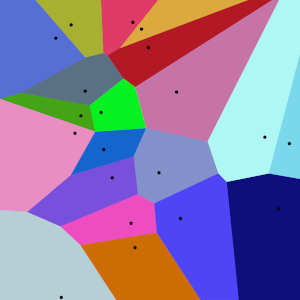
\includegraphics[width=5cm,height=\textheight,keepaspectratio,alt={Voronoi-Diagramm: Jede Fläche enthält die Punkte, die ihrem Mittelpunkt am nächsten liegen. Bild: Balu Ertl, CC BY-SA 4.0}]{bilder/biomes_voronoi.png}
\caption{Voronoi-Diagramm: Jede Fläche enthält die Punkte, die ihrem
Mittelpunkt am nächsten liegen. Bild: Balu Ertl, CC BY-SA 4.0}
\end{figure}

Wärme- und Feuchtigkeitswerte lassen sich leichter feinabstimmen, wenn
du die Beziehungen zwischen deinen Biomen sichtbar machst. Das ist
besonders wichtig, wenn du einen kompletten eigenen Satz an Biomen
erstellst, kann aber auch beim Ergänzen eines bestehenden Satzes helfen.

Am einfachsten machst du sichtbar, welche Biome aneinandergrenzen
können, mit einem
Voronoi-Diagramm.\index{voronoi-diagramm@Voronoi-Diagramm} Es zeigt für
jede Stelle eines zweidimensionalen Diagramms, welchem Punkt sie am
nächsten liegt.

Ein Voronoi-Diagramm zeigt, wo Biome, die aneinandergrenzen sollten, es
nicht tun -- und wo Biome aneinandergrenzen, die es nicht sollten.
Außerdem gibt es einen groben Eindruck davon, wie häufig Biome im Spiel
sein werden: Große und zentral liegende Biome sind häufiger als kleine
oder solche am Rand des Diagramms.

Dazu setzt du für jedes Biom einen Punkt anhand seiner Wärme und
Feuchtigkeit, mit der Wärme auf der x-Achse und der Feuchtigkeit auf der
y-Achse. Dann teilst du das Diagramm in Flächen ein, sodass jede Stelle
einer Fläche näher an deren Punkt liegt als an jedem anderen Punkt des
Diagramms.

Jede Fläche steht für ein Biom. Haben zwei Flächen eine gemeinsame
Grenze, können die zugehörigen Biome im Spiel nebeneinander liegen. Wie
lang die gemeinsame Grenze im Vergleich zu den Grenzen mit anderen
Flächen ist, verrät, wie häufig die beiden Biome voraussichtlich
nebeneinander vorkommen.

\subsection{Voronoi-Diagramme mit GeoGebra
erstellen}\label{voronoi-diagramme-mit-geogebra-erstellen}

Voronoi-Diagramme kannst du von Hand zeichnen oder mit Programmen wie
GeoGebra\footnote{\url{https://www.geogebra.org}} erstellen.

\begin{enumerate}
\def\labelenumi{\arabic{enumi}.}
\item
  Lege Punkte an, indem du in der Werkzeugleiste das Punktwerkzeug
  wählst (Symbol: ein Punkt mit „A``) und in das Diagramm klickst. Du
  kannst Punkte verschieben oder ihre Position in der linken
  Seitenleiste genau eingeben. Gib jedem Punkt außerdem eine
  Beschriftung, das macht es übersichtlicher.
\item
  Erzeuge dann das Voronoi-Diagramm, indem du in das Eingabefeld der
  linken Seitenleiste diese Funktion eingibst:

\begin{Shaded}
\begin{Highlighting}[]
\NormalTok{Voronoi(\{ A, B, C, D, E \})}
\end{Highlighting}
\end{Shaded}

  In den geschweiften Klammern stehen alle Punkte, durch Kommas
  getrennt.
\item
  Fertig! Du hast jetzt ein Voronoi-Diagramm, dessen Punkte du
  verschieben kannst.
\end{enumerate}

\section{Ein Biom registrieren}\label{ein-biom-registrieren}

Der folgende Code registriert ein einfaches Biom namens
\texttt{grasslands}:

\begin{Shaded}
\begin{Highlighting}[]
\VariableTok{core}\OperatorTok{.}\NormalTok{register\_biome}\OperatorTok{(\{}
    \VariableTok{name} \OperatorTok{=} \StringTok{"grasslands"}\OperatorTok{,}
    \VariableTok{node\_top} \OperatorTok{=} \StringTok{"default:dirt\_with\_grass"}\OperatorTok{,}
    \VariableTok{depth\_top} \OperatorTok{=} \DecValTok{1}\OperatorTok{,}
    \VariableTok{node\_filler} \OperatorTok{=} \StringTok{"default:dirt"}\OperatorTok{,}
    \VariableTok{depth\_filler} \OperatorTok{=} \DecValTok{3}\OperatorTok{,}
    \VariableTok{y\_max} \OperatorTok{=} \DecValTok{1000}\OperatorTok{,}
    \VariableTok{y\_min} \OperatorTok{=} \OperatorTok{{-}}\DecValTok{3}\OperatorTok{,}
    \VariableTok{heat\_point} \OperatorTok{=} \DecValTok{50}\OperatorTok{,}
    \VariableTok{humidity\_point} \OperatorTok{=} \DecValTok{50}\OperatorTok{,}
\OperatorTok{\})}
\end{Highlighting}
\end{Shaded}

Dieses Biom hat an der Oberfläche eine Schicht „Erde mit Gras`` und
darunter drei Schichten Erde. Es gibt keinen Stein-Node an; unter der
Erde liegt daher der Node, der als Mapgen-Alias
\texttt{mapgen\_\allowbreak{}stone} registriert ist.

Beim Registrieren eines Bioms gibt es viele Optionen; sie sind wie immer
in der Lua-API-Referenz\footnote{\url{https://api.luanti.org/definition-tables/\#biome-definition}}
dokumentiert.

Du musst nicht für jedes Biom jede Option angeben. Fehlt aber eine
bestimmte Option oder ein passender Mapgen-Alias, kann es zu Fehlern bei
der Kartengenerierung kommen.

\section{Was sind Dekorationen?}\label{was-sind-dekorationen}

Dekorationen sind Nodes oder Schematics, die bei der Kartengenerierung
auf der Karte platziert werden. Typische Beispiele sind Blumen, Büsche
und Bäume. Kreativere Einsätze sind etwa Eiszapfen oder Stalagmiten in
Höhlen, unterirdische Kristallformationen oder sogar kleine Gebäude.

Dekorationen lassen sich auf bestimmte Biome, Höhen oder
Untergrund-Nodes beschränken. Oft gestalten sie die Umgebung eines
Bioms, indem sie für bestimmte Pflanzen, Bäume oder andere Merkmale
sorgen.

\section{Eine einfache Dekoration
registrieren}\label{eine-einfache-dekoration-registrieren}

Einfache Dekorationen platzieren bei der Kartengenerierung einzelne
Nodes. Du gibst an, welcher Node als Dekoration platziert wird, wo er
platziert werden darf und wie häufig er vorkommt.

Zum Beispiel:

\begin{Shaded}
\begin{Highlighting}[]
\VariableTok{core}\OperatorTok{.}\NormalTok{register\_decoration}\OperatorTok{(\{}
    \VariableTok{deco\_type} \OperatorTok{=} \StringTok{"simple"}\OperatorTok{,}
    \VariableTok{place\_on} \OperatorTok{=} \OperatorTok{\{} \StringTok{"base:dirt\_with\_grass"} \OperatorTok{\},}
    \VariableTok{sidelen} \OperatorTok{=} \DecValTok{16}\OperatorTok{,}
    \VariableTok{fill\_ratio} \OperatorTok{=} \DecValTok{0.1}\OperatorTok{,}
    \VariableTok{biomes} \OperatorTok{=} \OperatorTok{\{} \StringTok{"grassy\_plains"} \OperatorTok{\},}
    \VariableTok{y\_max} \OperatorTok{=} \DecValTok{200}\OperatorTok{,}
    \VariableTok{y\_min} \OperatorTok{=} \DecValTok{1}\OperatorTok{,}
    \VariableTok{decoration} \OperatorTok{=} \StringTok{"plants:grass"}\OperatorTok{,}
\OperatorTok{\})}
\end{Highlighting}
\end{Shaded}

Hier wird der Node \texttt{plants:grass} im Biom
\texttt{grassy\_\allowbreak{}plains} auf
\texttt{base:dirt\_\allowbreak{}with\_\allowbreak{}grass} platziert,
zwischen den Höhen \texttt{y = 1} und \texttt{y = 200}.

\texttt{fill\_\allowbreak{}ratio} bestimmt, wie häufig die Dekoration
vorkommt; höhere Werte bis 1 führen zu sehr vielen Dekorationen.
Alternativ kannst du die Platzierung über Rauschparameter (\emph{noise
parameters}) steuern.

\section{Eine Schematic-Dekoration
registrieren}\label{eine-schematic-dekoration-registrieren}

Schematic-Dekorationen funktionieren ganz ähnlich wie einfache
Dekorationen, platzieren aber eine Schematic statt eines einzelnen
Nodes. Zum Beispiel:

\begin{Shaded}
\begin{Highlighting}[]
\VariableTok{core}\OperatorTok{.}\NormalTok{register\_decoration}\OperatorTok{(\{}
    \VariableTok{deco\_type} \OperatorTok{=} \StringTok{"schematic"}\OperatorTok{,}
    \VariableTok{place\_on} \OperatorTok{=} \OperatorTok{\{} \StringTok{"base:desert\_sand"} \OperatorTok{\},}
    \VariableTok{sidelen} \OperatorTok{=} \DecValTok{16}\OperatorTok{,}
    \VariableTok{fill\_ratio} \OperatorTok{=} \DecValTok{0.0001}\OperatorTok{,}
    \VariableTok{biomes} \OperatorTok{=} \OperatorTok{\{} \StringTok{"desert"} \OperatorTok{\},}
    \VariableTok{y\_max} \OperatorTok{=} \DecValTok{200}\OperatorTok{,}
    \VariableTok{y\_min} \OperatorTok{=} \DecValTok{1}\OperatorTok{,}
    \VariableTok{schematic} \OperatorTok{=} \VariableTok{core}\OperatorTok{.}\NormalTok{get\_modpath}\OperatorTok{(}\StringTok{"plants"}\OperatorTok{)}
        \OperatorTok{..} \StringTok{"/schematics/cactus.mts"}\OperatorTok{,}
    \VariableTok{flags} \OperatorTok{=} \StringTok{"place\_center\_x, place\_center\_z"}\OperatorTok{,}
    \VariableTok{rotation} \OperatorTok{=} \StringTok{"random"}\OperatorTok{,}
\OperatorTok{\})}
\end{Highlighting}
\end{Shaded}

Hier wird die Schematic \texttt{cactus.\allowbreak{}mts} in Wüstenbiomen
platziert. Du musst den Pfad zu einer Schematic angeben; in diesem Fall
liegt sie in einem eigenen Schematic-Verzeichnis innerhalb des Mods.

Das Beispiel setzt außerdem Flags, um die Schematic mittig zu
platzieren, und eine zufällige Drehung. Zufällig gedrehte Schematics
sorgen für mehr Abwechslung, wenn sie nicht symmetrisch sind.

\section{Mapgen-Aliase}\label{mapgen-aliase}

Bestehende Spiele bringen bereits passende Mapgen-Aliase mit. Eigene
musst du nur registrieren, wenn du ein eigenes Spiel entwickelst.

Mapgen-Aliase geben dem Kartengenerator der Engine Informationen und
werden so registriert:

\begin{Shaded}
\begin{Highlighting}[]
\VariableTok{core}\OperatorTok{.}\NormalTok{register\_alias}\OperatorTok{(}\StringTok{"mapgen\_stone"}\OperatorTok{,} \StringTok{"base:smoke\_stone"}\OperatorTok{)}
\end{Highlighting}
\end{Shaded}

Mindestens diese solltest du registrieren:

\begin{itemize}
\tightlist
\item
  \texttt{mapgen\_\allowbreak{}stone}
\item
  \texttt{mapgen\_\allowbreak{}water\_\allowbreak{}source}
\item
  \texttt{mapgen\_\allowbreak{}river\_\allowbreak{}water\_\allowbreak{}source}
\end{itemize}

Legst du nicht für alle Biome Höhlenflüssigkeiten fest, solltest du
außerdem registrieren:

\begin{itemize}
\tightlist
\item
  \texttt{mapgen\_\allowbreak{}lava\_\allowbreak{}source}
\end{itemize}

\chapter{Lua Voxel Manipulators}
\label{ch:advmap/lvm}

Die Funktionen aus dem Kapitel Grundlegende
Kartenoperationen~(Kapitel~\ref{ch:map/environment}) sind bequem und
einfach zu benutzen, für große Bereiche aber ineffizient. Bei jedem
Aufruf von \texttt{set\_\allowbreak{}node} oder
\texttt{get\_\allowbreak{}node} muss dein Mod mit der Engine
kommunizieren. Das führt zu ständigen einzelnen Kopiervorgängen zwischen
Engine und Mod, was langsam ist und die Leistung deines Spiels schnell
verschlechtert. Ein \emph{Lua Voxel Manipulator} (LVM)\index{lvm@LVM}
kann hier die bessere Wahl sein.

\section{Konzept}\label{konzept}

Mit einem LVM lädst du große Bereiche der Karte in den Speicher deines
Mods. Diese Daten kannst du dann lesen und schreiben, ohne weiter mit
der Engine zu kommunizieren und ohne dass
Callbacks\index{callback@Callback} laufen -- diese Operationen sind also
sehr schnell. Danach schreibst du den Bereich zurück in die Engine und
lässt die Beleuchtung berechnen.

\section{Daten in den LVM lesen}\label{daten-in-den-lvm-lesen}

In einen LVM kannst du nur einen Quader laden. Du musst also die
kleinste und größte Position ermitteln, die du verändern willst. Dann
erzeugst du einen LVM und liest den Bereich ein, zum Beispiel so:

\begin{Shaded}
\begin{Highlighting}[]
\KeywordTok{local} \VariableTok{vm} \OperatorTok{=} \VariableTok{core}\OperatorTok{.}\NormalTok{get\_voxel\_manip}\OperatorTok{()}
\KeywordTok{local} \VariableTok{emin}\OperatorTok{,} \VariableTok{emax} \OperatorTok{=} \VariableTok{vm}\OperatorTok{:}\NormalTok{read\_from\_map}\OperatorTok{(}\VariableTok{pos1}\OperatorTok{,} \VariableTok{pos2}\OperatorTok{)}
\end{Highlighting}
\end{Shaded}

Aus Leistungsgründen liest ein LVM fast nie genau den angegebenen
Bereich, sondern meist einen größeren. Diesen größeren Bereich geben
\texttt{emin} und \texttt{emax} an (\emph{emerged min pos} und
\emph{emerged max pos}). Der LVM lädt den Bereich für dich -- egal ob
dafür aus dem Arbeitsspeicher, von der Festplatte gelesen oder der
Kartengenerator\index{kartengenerierung@Kartengenerierung} aufgerufen
werden muss.

\begin{hinweis}{LVMs und Kartengenerierung}

Verwende
\texttt{core.\allowbreak{}get\_\allowbreak{}voxel\_\allowbreak{}manip()}\index{core@\texttt{core}!get_voxel_manip@\texttt{core.\allowbreak{}get\_\allowbreak{}voxel\_\allowbreak{}manip}}
nicht in der Kartengenerierung, das kann zu Fehlern führen. Verwende
dort stattdessen
\texttt{core.\allowbreak{}get\_\allowbreak{}mapgen\_\allowbreak{}object(\textquotedbl{}voxelmanip\textquotedbl{})}\index{core@\texttt{core}!get_mapgen_object@\texttt{core.\allowbreak{}get\_\allowbreak{}mapgen\_\allowbreak{}object}}.

\end{hinweis}

\section{Nodes lesen}\label{nodes-lesen}

Um die Node-Typen an bestimmten Positionen zu lesen, verwendest du
\texttt{get\_\allowbreak{}data()}. Die Methode gibt ein flaches Array
zurück, in dem jeder Eintrag für den Typ eines Nodes steht.

\begin{Shaded}
\begin{Highlighting}[]
\KeywordTok{local} \VariableTok{data} \OperatorTok{=} \VariableTok{vm}\OperatorTok{:}\NormalTok{get\_data}\OperatorTok{()}
\end{Highlighting}
\end{Shaded}

\texttt{param2} und Lichtwerte erhältst du mit
\texttt{get\_\allowbreak{}light\_\allowbreak{}data()} und
\texttt{get\_\allowbreak{}param2\_\allowbreak{}data()}.

Mit \texttt{emin} und \texttt{emax} berechnest du, wo ein Node in diesen
flachen Arrays liegt. Die Hilfsklasse
\texttt{VoxelArea}\index{voxelarea@\texttt{VoxelArea}} übernimmt die
Berechnung für dich.

\begin{Shaded}
\begin{Highlighting}[]
\KeywordTok{local} \VariableTok{a} \OperatorTok{=} \VariableTok{VoxelArea}\OperatorTok{:}\NormalTok{new}\OperatorTok{(\{}
    \VariableTok{MinEdge} \OperatorTok{=} \VariableTok{emin}\OperatorTok{,}
    \VariableTok{MaxEdge} \OperatorTok{=} \VariableTok{emax}\OperatorTok{,}
\OperatorTok{\})}

\CommentTok{{-}{-} Index des Nodes ermitteln}
\KeywordTok{local} \VariableTok{idx} \OperatorTok{=} \VariableTok{a}\OperatorTok{:}\NormalTok{index}\OperatorTok{(}\VariableTok{x}\OperatorTok{,} \VariableTok{y}\OperatorTok{,} \VariableTok{z}\OperatorTok{)}

\CommentTok{{-}{-} Node lesen}
\FunctionTok{print}\OperatorTok{(}\VariableTok{data}\OperatorTok{[}\VariableTok{idx}\OperatorTok{])}
\end{Highlighting}
\end{Shaded}

Dabei fällt auf, dass \texttt{data[idx]} eine ganze Zahl ist. Die Engine
speichert Nodes aus Leistungsgründen nicht als Strings, sondern als
Zahl, die \emph{Content-ID\index{content-id@Content-ID}} heißt. Die
Content-ID eines Node-Typs erhältst du mit
\texttt{get\_\allowbreak{}content\_\allowbreak{}id()}:

\begin{Shaded}
\begin{Highlighting}[]
\KeywordTok{local} \VariableTok{c\_stone} \OperatorTok{=} \VariableTok{core}\OperatorTok{.}\NormalTok{get\_content\_id}\OperatorTok{(}\StringTok{"default:stone"}\OperatorTok{)}
\end{Highlighting}
\end{Shaded}

Dann kannst du prüfen, ob der Node Stein ist:

\begin{Shaded}
\begin{Highlighting}[]
\KeywordTok{local} \VariableTok{idx} \OperatorTok{=} \VariableTok{a}\OperatorTok{:}\NormalTok{index}\OperatorTok{(}\VariableTok{x}\OperatorTok{,} \VariableTok{y}\OperatorTok{,} \VariableTok{z}\OperatorTok{)}
\ControlFlowTok{if} \VariableTok{data}\OperatorTok{[}\VariableTok{idx}\OperatorTok{]} \OperatorTok{==} \VariableTok{c\_stone} \ControlFlowTok{then}
    \FunctionTok{print}\OperatorTok{(}\StringTok{"Ist Stein!"}\OperatorTok{)}
\ControlFlowTok{end}
\end{Highlighting}
\end{Shaded}

Die Content-IDs von Node-Typen können sich während der Ladezeit noch
ändern. Ermittle sie deshalb nicht während dieser Zeit.

Die Nodes im Datenarray eines LVM liegen in umgekehrter
Koordinatenreihenfolge. Iteriere deshalb immer in der Reihenfolge
\texttt{z, y, x}:

\begin{Shaded}
\begin{Highlighting}[]
\ControlFlowTok{for} \VariableTok{z} \OperatorTok{=} \VariableTok{pos1}\OperatorTok{.}\VariableTok{z}\OperatorTok{,} \VariableTok{pos2}\OperatorTok{.}\VariableTok{z} \ControlFlowTok{do}
    \ControlFlowTok{for} \VariableTok{y} \OperatorTok{=} \VariableTok{pos1}\OperatorTok{.}\VariableTok{y}\OperatorTok{,} \VariableTok{pos2}\OperatorTok{.}\VariableTok{y} \ControlFlowTok{do}
        \ControlFlowTok{for} \VariableTok{x} \OperatorTok{=} \VariableTok{pos1}\OperatorTok{.}\VariableTok{x}\OperatorTok{,} \VariableTok{pos2}\OperatorTok{.}\VariableTok{x} \ControlFlowTok{do}
            \CommentTok{{-}{-} vi (voxel index) ist ein üblicher Name}
            \KeywordTok{local} \VariableTok{vi} \OperatorTok{=} \VariableTok{a}\OperatorTok{:}\NormalTok{index}\OperatorTok{(}\VariableTok{x}\OperatorTok{,} \VariableTok{y}\OperatorTok{,} \VariableTok{z}\OperatorTok{)}
            \ControlFlowTok{if} \VariableTok{data}\OperatorTok{[}\VariableTok{vi}\OperatorTok{]} \OperatorTok{==} \VariableTok{c\_stone} \ControlFlowTok{then}
                \FunctionTok{print}\OperatorTok{(}\StringTok{"Ist Stein!"}\OperatorTok{)}
            \ControlFlowTok{end}
        \ControlFlowTok{end}
    \ControlFlowTok{end}
\ControlFlowTok{end}
\end{Highlighting}
\end{Shaded}

Der Grund dafür liegt in der Rechnerarchitektur. Aus dem Arbeitsspeicher
zu lesen, ist recht teuer, deshalb haben Prozessoren mehrere
Cache-Ebenen. Liegen die angeforderten Daten im Cache, sind sie sehr
schnell verfügbar. Liegen sie nicht dort, kommt es zu einem
\emph{Cache-Miss}, und die Daten werden aus dem Arbeitsspeicher geholt.
Dabei werden auch die umliegenden Daten mitgeholt und ersetzen Daten im
Cache, weil das Programm sehr wahrscheinlich bald Daten aus der Nähe
anfordert. Eine gute Optimierungsregel ist daher, Daten der Reihe nach
zu lesen und \emph{Cache-Thrashing} zu vermeiden.

\section{Nodes schreiben}\label{nodes-schreiben}

Zuerst setzt du die neue Content-ID im Datenarray:

\begin{Shaded}
\begin{Highlighting}[]
\KeywordTok{local} \VariableTok{c\_air} \OperatorTok{=} \VariableTok{core}\OperatorTok{.}\NormalTok{get\_content\_id}\OperatorTok{(}\StringTok{"air"}\OperatorTok{)}

\ControlFlowTok{for} \VariableTok{z} \OperatorTok{=} \VariableTok{pos1}\OperatorTok{.}\VariableTok{z}\OperatorTok{,} \VariableTok{pos2}\OperatorTok{.}\VariableTok{z} \ControlFlowTok{do}
    \ControlFlowTok{for} \VariableTok{y} \OperatorTok{=} \VariableTok{pos1}\OperatorTok{.}\VariableTok{y}\OperatorTok{,} \VariableTok{pos2}\OperatorTok{.}\VariableTok{y} \ControlFlowTok{do}
        \ControlFlowTok{for} \VariableTok{x} \OperatorTok{=} \VariableTok{pos1}\OperatorTok{.}\VariableTok{x}\OperatorTok{,} \VariableTok{pos2}\OperatorTok{.}\VariableTok{x} \ControlFlowTok{do}
            \KeywordTok{local} \VariableTok{vi} \OperatorTok{=} \VariableTok{a}\OperatorTok{:}\NormalTok{index}\OperatorTok{(}\VariableTok{x}\OperatorTok{,} \VariableTok{y}\OperatorTok{,} \VariableTok{z}\OperatorTok{)}
            \ControlFlowTok{if} \VariableTok{data}\OperatorTok{[}\VariableTok{vi}\OperatorTok{]} \OperatorTok{==} \VariableTok{c\_stone} \ControlFlowTok{then}
                \VariableTok{data}\OperatorTok{[}\VariableTok{vi}\OperatorTok{]} \OperatorTok{=} \VariableTok{c\_air}
            \ControlFlowTok{end}
        \ControlFlowTok{end}
    \ControlFlowTok{end}
\ControlFlowTok{end}
\end{Highlighting}
\end{Shaded}

Bist du mit dem Setzen fertig, lädst du das Datenarray zurück in die
Engine:

\begin{Shaded}
\begin{Highlighting}[]
\VariableTok{vm}\OperatorTok{:}\NormalTok{set\_data}\OperatorTok{(}\VariableTok{data}\OperatorTok{)}
\VariableTok{vm}\OperatorTok{:}\NormalTok{write\_to\_map}\OperatorTok{(}\KeywordTok{true}\OperatorTok{)}
\end{Highlighting}
\end{Shaded}

Für Licht- und \texttt{param2}-Daten gibt es die passend benannten
Methoden \texttt{set\_\allowbreak{}light\_\allowbreak{}data()} und
\texttt{set\_\allowbreak{}param2\_\allowbreak{}data()}.

\texttt{write\_\allowbreak{}to\_\allowbreak{}map()} erwartet einen
Wahrheitswert: \texttt{true}, wenn die Beleuchtung berechnet werden
soll. Übergibst du \texttt{false}, musst du die Beleuchtung später mit
\texttt{core.\allowbreak{}fix\_\allowbreak{}light}\index{core@\texttt{core}!fix_light@\texttt{core.\allowbreak{}fix\_\allowbreak{}light}}
neu berechnen.

\section{Beispiel}\label{beispiel}

\begin{Shaded}
\begin{Highlighting}[]
\KeywordTok{local} \KeywordTok{function}\NormalTok{ grass\_to\_dirt}\OperatorTok{(}\VariableTok{pos1}\OperatorTok{,} \VariableTok{pos2}\OperatorTok{)}
    \KeywordTok{local} \VariableTok{c\_dirt} \OperatorTok{=} \VariableTok{core}\OperatorTok{.}\NormalTok{get\_content\_id}\OperatorTok{(}\StringTok{"default:dirt"}\OperatorTok{)}
    \KeywordTok{local} \VariableTok{c\_grass} \OperatorTok{=}
        \VariableTok{core}\OperatorTok{.}\NormalTok{get\_content\_id}\OperatorTok{(}\StringTok{"default:dirt\_with\_grass"}\OperatorTok{)}

    \CommentTok{{-}{-} Daten in den LVM lesen}
    \KeywordTok{local} \VariableTok{vm} \OperatorTok{=} \VariableTok{core}\OperatorTok{.}\NormalTok{get\_voxel\_manip}\OperatorTok{()}
    \KeywordTok{local} \VariableTok{emin}\OperatorTok{,} \VariableTok{emax} \OperatorTok{=} \VariableTok{vm}\OperatorTok{:}\NormalTok{read\_from\_map}\OperatorTok{(}\VariableTok{pos1}\OperatorTok{,} \VariableTok{pos2}\OperatorTok{)}
    \KeywordTok{local} \VariableTok{a} \OperatorTok{=} \VariableTok{VoxelArea}\OperatorTok{:}\NormalTok{new}\OperatorTok{(\{}
        \VariableTok{MinEdge} \OperatorTok{=} \VariableTok{emin}\OperatorTok{,}
        \VariableTok{MaxEdge} \OperatorTok{=} \VariableTok{emax}\OperatorTok{,}
    \OperatorTok{\})}
    \KeywordTok{local} \VariableTok{data} \OperatorTok{=} \VariableTok{vm}\OperatorTok{:}\NormalTok{get\_data}\OperatorTok{()}

    \CommentTok{{-}{-} Daten ändern}
    \ControlFlowTok{for} \VariableTok{z} \OperatorTok{=} \VariableTok{pos1}\OperatorTok{.}\VariableTok{z}\OperatorTok{,} \VariableTok{pos2}\OperatorTok{.}\VariableTok{z} \ControlFlowTok{do}
        \ControlFlowTok{for} \VariableTok{y} \OperatorTok{=} \VariableTok{pos1}\OperatorTok{.}\VariableTok{y}\OperatorTok{,} \VariableTok{pos2}\OperatorTok{.}\VariableTok{y} \ControlFlowTok{do}
            \ControlFlowTok{for} \VariableTok{x} \OperatorTok{=} \VariableTok{pos1}\OperatorTok{.}\VariableTok{x}\OperatorTok{,} \VariableTok{pos2}\OperatorTok{.}\VariableTok{x} \ControlFlowTok{do}
                \KeywordTok{local} \VariableTok{vi} \OperatorTok{=} \VariableTok{a}\OperatorTok{:}\NormalTok{index}\OperatorTok{(}\VariableTok{x}\OperatorTok{,} \VariableTok{y}\OperatorTok{,} \VariableTok{z}\OperatorTok{)}
                \ControlFlowTok{if} \VariableTok{data}\OperatorTok{[}\VariableTok{vi}\OperatorTok{]} \OperatorTok{==} \VariableTok{c\_grass} \ControlFlowTok{then}
                    \VariableTok{data}\OperatorTok{[}\VariableTok{vi}\OperatorTok{]} \OperatorTok{=} \VariableTok{c\_dirt}
                \ControlFlowTok{end}
            \ControlFlowTok{end}
        \ControlFlowTok{end}
    \ControlFlowTok{end}

    \CommentTok{{-}{-} Daten schreiben}
    \VariableTok{vm}\OperatorTok{:}\NormalTok{set\_data}\OperatorTok{(}\VariableTok{data}\OperatorTok{)}
    \VariableTok{vm}\OperatorTok{:}\NormalTok{write\_to\_map}\OperatorTok{(}\KeywordTok{true}\OperatorTok{)}
\KeywordTok{end}
\end{Highlighting}
\end{Shaded}

\section{Jetzt bist du dran}\label{jetzt-bist-du-dran}

\begin{itemize}
\tightlist
\item
  Schreibe
  \texttt{replace\_\allowbreak{}in\_\allowbreak{}area(from, to, pos1, pos2)},
  das im angegebenen Bereich jedes Vorkommen von \texttt{from} durch
  \texttt{to} ersetzt; \texttt{from} und \texttt{to} sind Node-Namen.
\item
  Schreibe eine Funktion, die alle Truhen um 90° dreht.
\item
  Schreibe eine Funktion, die mit einem LVM bemoosten Bruchstein auf
  benachbarten Stein und Bruchstein übergreifen lässt. Breitet sich der
  Moosbewuchs bei deiner Umsetzung jedes Mal weiter als einen Node aus?
  Wenn ja, wie könntest du das verhindern?
\end{itemize}


\part{Spiele}
\chapter{Spiele erstellen}
\label{ch:games/games}

Die Stärke von Luanti liegt darin, dass sich Spiele einfach entwickeln
lassen, ohne eigene Voxel-Grafik, Voxel-Algorithmen oder ausgefeilten
Netzwerkcode schreiben zu müssen.

\section{Was ist ein Spiel?}\label{was-ist-ein-spiel}

Ein Spiel ist eine Sammlung von Mods, die zusammen ein stimmiges Ganzes
ergeben. Ein gutes Spiel hat ein durchgängiges Thema und eine Richtung:
Es kann zum Beispiel ein klassisches Bau- und Abbauspiel mit harten
Überlebenselementen sein oder eine Weltraumsimulation mit
Steampunk-Automatisierung.

Spieldesign ist ein komplexes Thema und ein eigenes Fachgebiet. Dieses
Buch kann es nur kurz streifen.

\section{Spielverzeichnis}\label{spielverzeichnis}

Aufbau und Ort eines Spiels kommen dir nach der Arbeit mit Mods recht
vertraut vor. Spiele liegen in einem Spielverzeichnis, etwa
\texttt{minetest/\allowbreak{}games/\allowbreak{}foo\_\allowbreak{}game}.

\begin{Shaded}
\begin{Highlighting}[]
\NormalTok{foo\_game}
\NormalTok{├── game.conf}
\NormalTok{├── menu}
\NormalTok{│   ├── header.png}
\NormalTok{│   ├── background.png}
\NormalTok{│   └── icon.png}
\NormalTok{├── minetest.conf}
\NormalTok{├── mods}
\NormalTok{│   └── ... Mods}
\NormalTok{├── README.txt}
\NormalTok{└── settingtypes.txt}
\end{Highlighting}
\end{Shaded}

Nötig ist nur der Ordner \texttt{mods};
\texttt{game.\allowbreak{}conf}\index{game.conf@\texttt{game.\allowbreak{}conf}}
und \texttt{menu/\allowbreak{}icon.\allowbreak{}png} werden aber
empfohlen. Eine einfache \texttt{game.\allowbreak{}conf} sieht so aus:

\begin{Shaded}
\begin{Highlighting}[]
\NormalTok{title = Foo Game}
\NormalTok{description = Ein Spiel über Foo.}
\end{Highlighting}
\end{Shaded}

\section{Kompatibilität zwischen
Spielen}\label{kompatibilituxe4t-zwischen-spielen}

\subsection{API-Kompatibilität}\label{api-kompatibilituxe4t}

Es lohnt sich, so viel API-Kompatibilität mit Minetest Game zu wahren,
wie es sich einrichten lässt. Dann lassen sich Mods viel leichter auf
ein anderes Spiel übertragen.

Am besten wahrst du die Kompatibilität mit einem anderen Spiel, indem du
die API-Kompatibilität mit gleichnamigen Mods wahrst. Trägt ein Mod
denselben Namen wie ein anderer -- auch wie ein Mod von Dritten --,
sollte er also eine kompatible API haben. Enthält ein Spiel zum Beispiel
einen Mod namens \texttt{doors}, sollte er dieselbe API haben wie
\texttt{doors} in Minetest Game.

Die API-Kompatibilität eines Mods setzt sich zusammen aus:

\begin{itemize}
\tightlist
\item
  der Lua-API-Tabelle -- alle dokumentierten oder beworbenen Funktionen
  in der gleichnamigen globalen Tabelle, zum Beispiel
  \texttt{mobs.\allowbreak{}register\_\allowbreak{}mob};
\item
  den registrierten Nodes und Items -- also dass diese vorhanden sind.
\end{itemize}

Kleine Brüche sind nicht so schlimm, etwa wenn eine beiläufige
Hilfsfunktion fehlt, die eigentlich nur intern verwendet wurde. Größere
Brüche bei Kernfunktionen sind dagegen sehr schlecht.

Mit einem riesigen Alleskönner-Mod wie \emph{default} in Minetest Game
ist API-Kompatibilität kaum zu wahren. In diesem Fall sollte das Spiel
keinen Mod namens \texttt{default} enthalten.

API-Kompatibilität betrifft auch andere Mods und Spiele von Dritten.
Achte also darauf, dass neue Mods einen eindeutigen Namen haben. Ob ein
Mod-Name schon vergeben ist, findest du mit einer Suche auf
\url{https://content.luanti.org/} heraus.

\subsection{Gruppen und Aliase}\label{gruppen-und-aliase}

Gruppen\index{gruppe@Gruppe} und Aliase\index{alias@Alias} helfen beide,
die Kompatibilität zwischen Spielen zu wahren, denn mit ihnen dürfen
sich Itemnamen zwischen Spielen unterscheiden. Häufige Nodes wie Stein
und Holz sollten Gruppen haben, die das Material angeben. Es ist
außerdem sinnvoll, Aliase von \texttt{default}-Nodes auf ihre direkten
Entsprechungen anzulegen.

\section{Jetzt bist du dran}\label{jetzt-bist-du-dran}

\begin{itemize}
\tightlist
\item
  Erstelle ein einfaches Spiel, in dem der Spieler Punkte bekommt, wenn
  er besondere Blöcke abbaut.
\end{itemize}


\part{Qualität}
\chapter{Übersetzungen}
\label{ch:quality/translations}

Wenn deine Mods und Spiele übersetzt werden können, haben mehr Menschen
Freude daran. Laut Google Play haben 64 \% der Luanti-Nutzer unter
Android nicht Englisch als Hauptsprache. Für alle Plattformen zusammen
erhebt Luanti keine Statistik zu den Sprachen der Nutzer, aber der
Anteil nicht englischsprachiger Spieler dürfte hoch sein.

In Luanti schreibst du deine Texte auf Englisch und bildest sie mit
Übersetzungsdateien auf andere Sprachen ab. Übersetzt wird auf dem
Client jedes Spielers, sodass jeder Spieler eine andere Sprache sehen
kann.

\section{Wie funktioniert die Übersetzung auf dem
Client?}\label{wie-funktioniert-die-uxfcbersetzung-auf-dem-client}

\subsection{Markierter Text}\label{markierter-text}

Der Server muss den Clients mitteilen, wie Text übersetzt werden soll.
Dazu werden Steuerzeichen in den Text eingefügt, die Luanti sagen, wo
und wie übersetzt werden soll. Das nennt man \emph{markierten Text}
(\emph{marked up text}); dazu später mehr.

Um Text als übersetzbar zu markieren, verwendest du eine
Übersetzerfunktion (\texttt{S()}), die du mit
\texttt{core.\allowbreak{}get\_\allowbreak{}translator(textdomain)}\index{core@\texttt{core}!get_translator@\texttt{core.\allowbreak{}get\_\allowbreak{}translator}}
erhältst:

\begin{Shaded}
\begin{Highlighting}[]
\KeywordTok{local} \ConstantTok{S} \OperatorTok{=} \VariableTok{core}\OperatorTok{.}\NormalTok{get\_translator}\OperatorTok{(}\StringTok{"mymod"}\OperatorTok{)}

\VariableTok{core}\OperatorTok{.}\NormalTok{register\_craftitem}\OperatorTok{(}\StringTok{"mymod:item"}\OperatorTok{,} \OperatorTok{\{}
    \VariableTok{description} \OperatorTok{=}\NormalTok{ S}\OperatorTok{(}\StringTok{"My Item"}\OperatorTok{),}
\OperatorTok{\})}
\end{Highlighting}
\end{Shaded}

Das erste Argument von \texttt{get\_\allowbreak{}translator} ist die
\emph{Textdomain\index{textdomain@Textdomain}}, eine Art
Namensraum.\index{namensraum@Namensraum} Statt alle Übersetzungen einer
Sprache in einer Datei zu sammeln, werden sie nach Textdomains getrennt,
mit einer Datei je Textdomain und Sprache. Die Textdomain sollte dem
Mod-Namen entsprechen, um Konflikte zwischen Mods zu vermeiden.

Markierten Text kannst du fast überall verwenden, wo lesbarer Text
erwartet wird, etwa in Formspecs,\index{formspec@Formspec} Feldern von
Item-Definitionen, \texttt{infotext} und vielem mehr. In Formspecs musst
du markierten Text mit
\texttt{core.\allowbreak{}formspec\_\allowbreak{}escape}\index{core@\texttt{core}!formspec_escape@\texttt{core.\allowbreak{}formspec\_\allowbreak{}escape}}
maskieren.

Trifft der Client auf übersetzbaren Text, etwa in \texttt{description},
sucht er ihn in der Übersetzungsdatei für die Sprache des Spielers.
Findet er keine Übersetzung, verwendet er den englischen Text.

Übersetzbarer markierter Text enthält den englischen Ausgangstext, die
Textdomain und alle weiteren Argumente von \texttt{S()}. Er ist im
Grunde eine Textkodierung des \texttt{S}-Aufrufs mit allen nötigen
Informationen.

Eine weitere Art markierten Texts liefert
\texttt{core.\allowbreak{}colorize}\index{core@\texttt{core}!colorize@\texttt{core.\allowbreak{}colorize}}.

\begin{hinweis}{Kodierung von markiertem Text}

Das genaue Format von markiertem Text musst du nicht kennen, es hilft
aber beim Verständnis.

\begin{Shaded}
\begin{Highlighting}[]
\NormalTok{"\textbackslash{}27(T@mymod)Hello everyone!\textbackslash{}27E"}
\end{Highlighting}
\end{Shaded}

\begin{itemize}
\tightlist
\item
  \texttt{\textbackslash{}27} ist das Escape-Zeichen. Es sagt Luanti,
  dass etwas Besonderes folgt. Es wird sowohl für Übersetzungen als auch
  für das Einfärben von Text verwendet.
\item
  \texttt{(T@mymod)} besagt, dass der folgende Text mit der Textdomain
  \texttt{mymod} übersetzbar ist.
\item
  \texttt{Hello everyone!} ist der übersetzbare englische Text, wie er
  der Übersetzerfunktion übergeben wurde.
\item
  \texttt{\textbackslash{}27E} ist wieder das Escape-Zeichen, gefolgt
  von \texttt{E}; es markiert das Ende.
\end{itemize}

\end{hinweis}

\subsection{Übersetzungsdateien}\label{uxfcbersetzungsdateien}

Übersetzungsdateien sind Mediendateien im Ordner \texttt{locale} des
jeweiligen Mods.

Luanti unterstützt derzeit zwei Formate: \emph{gettext} und ein eigenes,
älteres Format. Seit Luanti 5.10 gibt es gettext, ein verbreitetes und
bewährtes Format. Wenn möglich, solltest du gettext verwenden. Einziger
Nachteil: Luanti-Clients vor Version 5.10 können damit noch nicht
umgehen.

Bei gettext erwartet Luanti Übersetzungsdateien im Format
\texttt{[textdomain].\allowbreak{}[sprache].\allowbreak{}po} im Ordner
\texttt{locale}. Zum Erstellen und Pflegen kannst du externe Werkzeuge
verwenden. Die Luanti-Dokumentation enthält einen Artikel über
Weblate\footnote{\url{https://docs.luanti.org/for-creators/translation/weblate/}}
(englisch).

Lies außerdem die offizielle Luanti-Dokumentation zu
Übersetzungen\footnote{\url{https://api.luanti.org/translations/}}
(englisch).

Um Strings automatisch aus deinem Quellcode zu ziehen und
\texttt{.\allowbreak{}pot}-Vorlagen zu erzeugen, kannst du
\texttt{gettext} installieren und diesen Befehl anpassen:

\begin{Shaded}
\begin{Highlighting}[]
\NormalTok{xgettext {-}L lua {-}kS {-}kPS:1,2 \textbackslash{}}
\NormalTok{  {-}kcore.translate:1c,2 {-}kcore.translate\_n:1c,2,3 \textbackslash{}}
\NormalTok{  {-}d your\_textdomain {-}o locale/your\_textdomain.pot *.lua}
\end{Highlighting}
\end{Shaded}

Für jeden verwendeten Funktionsnamen kannst du ein weiteres \texttt{-k}
angeben. Die Angaben nach dem Funktionsnamen betreffen Pluralformen;
Einzelheiten stehen im Handbuch von gettext.

\subsubsection{Altes Format}\label{altes-format}

Übersetzungsdateien im alten Format heißen
\texttt{[textdomain].\allowbreak{}[sprache].\allowbreak{}tr}.

Sie beginnen mit einem Kommentar, der die Textdomain angibt; die
weiteren Zeilen bilden den englischen Ausgangstext auf die Übersetzung
ab.

Zum Beispiel \texttt{mymod.\allowbreak{}de.\allowbreak{}tr}:

\begin{Shaded}
\begin{Highlighting}[]
\NormalTok{\# textdomain: mymod}
\NormalTok{Hello everyone!=Hallo zusammen!}
\NormalTok{I like grapefruit=Ich mag Grapefruit}
\end{Highlighting}
\end{Shaded}

Übersetzungsdateien solltest du aus dem Quellcode deines Mods oder
Spiels erzeugen, etwa mit update\_translations\footnote{\url{https://github.com/minetest-tools/update_translations}}.
Das Werkzeug sucht in deinem Lua-Code nach \texttt{S(} und erstellt
automatisch eine Vorlage, die Übersetzer in ihre Sprache übertragen
können. Es aktualisiert die Übersetzungsdateien auch, wenn sich dein
Quellcode ändert.

Schreib in \texttt{S()} immer wörtlichen Text (in
\texttt{\textquotedbl{}}) statt einer Variablen; so finden Werkzeuge die
zu übersetzenden Texte.

\section{Platzhalter}\label{platzhalter}

Oft müssen variable Informationen in einen übersetzbaren Text. Dabei
darf der Text nicht einfach verkettet werden, denn sonst können
Übersetzer die Reihenfolge der Variablen im Satz nicht ändern. Verwende
stattdessen das Platzhaltersystem der Übersetzung:

\begin{Shaded}
\begin{Highlighting}[]
\VariableTok{core}\OperatorTok{.}\NormalTok{register\_on\_joinplayer}\OperatorTok{(}\KeywordTok{function}\OperatorTok{(}\VariableTok{player}\OperatorTok{)}
    \VariableTok{core}\OperatorTok{.}\NormalTok{chat\_send\_all}\OperatorTok{(}
\NormalTok{        S}\OperatorTok{(}
            \StringTok{"Everyone, say hi to @1!"}\OperatorTok{,}
            \VariableTok{player}\OperatorTok{:}\NormalTok{get\_player\_name}\OperatorTok{()}
        \OperatorTok{)}
    \OperatorTok{)}
\KeywordTok{end}\OperatorTok{)}
\end{Highlighting}
\end{Shaded}

Ein wörtliches \texttt{@} schreibst du in einer Übersetzung als
\texttt{@@}.

Innerhalb eines Satzes solltest du nicht verketten, mehrere Sätze
verkettest du aber am besten. Das hilft Übersetzern, weil die Strings
kürzer bleiben.

\begin{Shaded}
\begin{Highlighting}[]
\NormalTok{S}\OperatorTok{(}\StringTok{"Hello @1!"}\OperatorTok{,} \VariableTok{player\_name}\OperatorTok{)}
    \OperatorTok{..} \StringTok{" "}
    \OperatorTok{..}\NormalTok{ S}\OperatorTok{(}\StringTok{"You have @1 new messages."}\OperatorTok{,} \OperatorTok{\#}\VariableTok{msgs}\OperatorTok{),}
\end{Highlighting}
\end{Shaded}

\section{Gute Praxis und verbreitete
Irrtümer}\label{gute-praxis-und-verbreitete-irrtuxfcmer}

\begin{itemize}
\tightlist
\item
  Verkette keinen Text, sondern verwende Platzhalter. So haben
  Übersetzer volle Kontrolle über die Reihenfolge.
\item
  Variablen verändern oft den umgebenden Text, etwa durch Geschlecht und
  Pluralbildung. Das ist schwer zu handhaben und wird deshalb oft
  übergangen oder mit geschlechtsneutralen Formulierungen umgangen.
\item
  Übersetzungen können viel länger oder kürzer sein als der englische
  Text. Lass genug Platz.
\item
  Andere Sprachen schreiben Zahlen womöglich anders, etwa mit Komma als
  Dezimaltrennzeichen: \texttt{1.\allowbreak{}000,23},
  \texttt{1'000'000,32}.
\item
  Geh nicht davon aus, dass andere Sprachen Groß- und Kleinschreibung
  genauso verwenden wie Englisch.
\end{itemize}

\section{Übersetzung auf dem
Server}\label{uxfcbersetzung-auf-dem-server}

Manchmal brauchst du die Übersetzung eines Textes auf dem Server, etwa
um Text zu sortieren oder zu durchsuchen. Die Sprache eines Spielers
erhältst du mit
\texttt{get\_\allowbreak{}player\_\allowbreak{}information}, und mit
\texttt{get\_\allowbreak{}translated\_\allowbreak{}string} übersetzt du
markierten Text.

\begin{Shaded}
\begin{Highlighting}[]
\KeywordTok{local} \VariableTok{list} \OperatorTok{=} \OperatorTok{\{}
\NormalTok{    S}\OperatorTok{(}\StringTok{"Hello world!"}\OperatorTok{),}
\NormalTok{    S}\OperatorTok{(}\StringTok{"Potato"}\OperatorTok{),}
\OperatorTok{\}}

\VariableTok{core}\OperatorTok{.}\NormalTok{register\_chatcommand}\OperatorTok{(}\StringTok{"find"}\OperatorTok{,} \OperatorTok{\{}
    \VariableTok{func} \OperatorTok{=} \KeywordTok{function}\OperatorTok{(}\VariableTok{name}\OperatorTok{,} \VariableTok{param}\OperatorTok{)}
        \KeywordTok{local} \VariableTok{info} \OperatorTok{=} \VariableTok{core}\OperatorTok{.}\NormalTok{get\_player\_information}\OperatorTok{(}\VariableTok{name}\OperatorTok{)}
        \KeywordTok{local} \VariableTok{language} \OperatorTok{=} \VariableTok{info} \KeywordTok{and} \VariableTok{info}\OperatorTok{.}\VariableTok{language} \KeywordTok{or} \StringTok{"en"}

        \ControlFlowTok{for} \ConstantTok{\_}\OperatorTok{,} \VariableTok{line} \KeywordTok{in} \FunctionTok{ipairs}\OperatorTok{(}\VariableTok{list}\OperatorTok{)} \ControlFlowTok{do}
            \KeywordTok{local} \VariableTok{trans} \OperatorTok{=}
                \VariableTok{core}\OperatorTok{.}\NormalTok{get\_translated\_string}\OperatorTok{(}\VariableTok{language}\OperatorTok{,} \VariableTok{line}\OperatorTok{)}
            \ControlFlowTok{if} \VariableTok{trans}\OperatorTok{:}\FunctionTok{find}\OperatorTok{(}\VariableTok{param}\OperatorTok{,} \DecValTok{1}\OperatorTok{,} \KeywordTok{true}\OperatorTok{)} \ControlFlowTok{then}
                \ControlFlowTok{return} \KeywordTok{true}\OperatorTok{,} \VariableTok{line}
            \ControlFlowTok{end}
        \ControlFlowTok{end}
        \ControlFlowTok{return} \KeywordTok{false}\OperatorTok{,}\NormalTok{ S}\OperatorTok{(}\StringTok{"Nothing found."}\OperatorTok{)}
    \KeywordTok{end}\OperatorTok{,}
\OperatorTok{\})}
\end{Highlighting}
\end{Shaded}

\section{Fazit}\label{fazit}

Mit der Übersetzungs-API machst du Mods und Spiele mehr Menschen
zugänglich. Sie richtig einzusetzen, erfordert aber etwas Sorgfalt.

\chapter{Häufige Fehler}
\label{ch:quality/common-mistakes}

Dieses Kapitel beschreibt häufige Fehler und wie du sie vermeidest.

\section{Vorsicht beim Speichern von
ObjectRefs}\label{vorsicht-beim-speichern-von-objectrefs}

Ein ObjectRef\index{objectref@\texttt{ObjectRef}} (also ein Spieler oder
eine Entity)\index{entity@Entity} wird ungültig, wenn der Spieler oder
die Entity, für die es steht, das Spiel verlässt. Das passiert, wenn der
Spieler offline geht oder die Entity entladen oder entfernt wird.

Seit Luanti 5.2 geben die Methoden eines ungültigen ObjectRefs immer
\texttt{nil} zurück; jeder Aufruf wird im Grunde ignoriert.

Speichere ObjectRefs möglichst nicht. Wenn du es doch tust, prüfe vor
der Verwendung, ob das ObjectRef noch gültig ist:

\begin{Shaded}
\begin{Highlighting}[]
\CommentTok{{-}{-} Funktioniert erst ab Luanti 5.2}
\ControlFlowTok{if} \VariableTok{obj}\OperatorTok{:}\NormalTok{get\_pos}\OperatorTok{()} \ControlFlowTok{then}
    \CommentTok{{-}{-} ist gültig!}
\ControlFlowTok{end}
\end{Highlighting}
\end{Shaded}

\section{Formspec-Eingaben nicht
vertrauen}\label{formspec-eingaben-nicht-vertrauen}

Bösartige Clients können Formspecs\index{formspec@Formspec} jederzeit
und mit beliebigem Inhalt abschicken.

Der folgende Code hat zum Beispiel eine Sicherheitslücke, durch die
Spieler sich selbst Moderatorrechte geben können:

\begin{Shaded}
\begin{Highlighting}[]
\KeywordTok{local} \KeywordTok{function}\NormalTok{ show\_formspec}\OperatorTok{(}\VariableTok{name}\OperatorTok{)}
    \ControlFlowTok{if}
        \KeywordTok{not} \VariableTok{core}\OperatorTok{.}\NormalTok{check\_player\_privs}\OperatorTok{(}\VariableTok{name}\OperatorTok{,} \OperatorTok{\{} \VariableTok{privs} \OperatorTok{=} \KeywordTok{true} \OperatorTok{\})}
    \ControlFlowTok{then}
        \ControlFlowTok{return} \KeywordTok{false}
    \ControlFlowTok{end}

    \VariableTok{core}\OperatorTok{.}\NormalTok{show\_formspec}\OperatorTok{(}
        \VariableTok{name}\OperatorTok{,}
        \StringTok{"modman:modman"}\OperatorTok{,}
        \VerbatimStringTok{[[}
\VerbatimStringTok{        size[3,2]}
\VerbatimStringTok{        field[0,0;3,1;target;Name;]}
\VerbatimStringTok{        button\_exit[0,1;3,1;sub;Promote]}
\VerbatimStringTok{    ]]}
    \OperatorTok{)}
    \ControlFlowTok{return} \KeywordTok{true}
\KeywordTok{end}

\VariableTok{core}\OperatorTok{.}\NormalTok{register\_on\_player\_receive\_fields}\OperatorTok{(}
    \KeywordTok{function}\OperatorTok{(}\VariableTok{player}\OperatorTok{,} \VariableTok{formname}\OperatorTok{,} \VariableTok{fields}\OperatorTok{)}
        \CommentTok{{-}{-} SCHLECHT! Hier fehlt die Prüfung der Privilegien!}

        \KeywordTok{local} \VariableTok{privs} \OperatorTok{=} \VariableTok{core}\OperatorTok{.}\NormalTok{get\_player\_privs}\OperatorTok{(}\VariableTok{fields}\OperatorTok{.}\VariableTok{target}\OperatorTok{)}
        \VariableTok{privs}\OperatorTok{.}\VariableTok{kick} \OperatorTok{=} \KeywordTok{true}
        \VariableTok{privs}\OperatorTok{.}\VariableTok{ban} \OperatorTok{=} \KeywordTok{true}
        \VariableTok{core}\OperatorTok{.}\NormalTok{set\_player\_privs}\OperatorTok{(}\VariableTok{fields}\OperatorTok{.}\VariableTok{target}\OperatorTok{,} \VariableTok{privs}\OperatorTok{)}
        \ControlFlowTok{return} \KeywordTok{true}
    \KeywordTok{end}
\OperatorTok{)}
\end{Highlighting}
\end{Shaded}

Mit einer Prüfung der Privilegien\index{privileg@Privileg} ist die Lücke
geschlossen:

\begin{Shaded}
\begin{Highlighting}[]
\VariableTok{core}\OperatorTok{.}\NormalTok{register\_on\_player\_receive\_fields}\OperatorTok{(}
    \KeywordTok{function}\OperatorTok{(}\VariableTok{player}\OperatorTok{,} \VariableTok{formname}\OperatorTok{,} \VariableTok{fields}\OperatorTok{)}
        \KeywordTok{local} \VariableTok{name} \OperatorTok{=} \VariableTok{player}\OperatorTok{:}\NormalTok{get\_player\_name}\OperatorTok{()}
        \ControlFlowTok{if}
            \KeywordTok{not} \VariableTok{core}\OperatorTok{.}\NormalTok{check\_player\_privs}\OperatorTok{(}
                \VariableTok{name}\OperatorTok{,}
                \OperatorTok{\{} \VariableTok{privs} \OperatorTok{=} \KeywordTok{true} \OperatorTok{\}}
            \OperatorTok{)}
        \ControlFlowTok{then}
            \ControlFlowTok{return} \KeywordTok{false}
        \ControlFlowTok{end}

        \CommentTok{{-}{-} Code}
    \KeywordTok{end}
\OperatorTok{)}
\end{Highlighting}
\end{Shaded}

\section{ItemStacks nach dem Ändern
zurücksetzen}\label{itemstacks-nach-dem-uxe4ndern-zuruxfccksetzen}

Ist dir aufgefallen, dass es in der API einfach
\texttt{ItemStack}\index{itemstack@\texttt{ItemStack}} heißt und nicht
\texttt{ItemStackRef}, analog zu \texttt{InvRef}? Ein \texttt{ItemStack}
ist nämlich keine Referenz, sondern eine Kopie. Du arbeitest mit einer
Kopie der Daten, nicht mit dem Stack im
Inventar.\index{inventar@Inventar} Änderst du den Stack, ändert sich der
Stack im Inventar also nicht.

Mach das zum Beispiel nicht:

\begin{Shaded}
\begin{Highlighting}[]
\KeywordTok{local} \VariableTok{inv} \OperatorTok{=} \VariableTok{player}\OperatorTok{:}\NormalTok{get\_inventory}\OperatorTok{()}
\KeywordTok{local} \VariableTok{stack} \OperatorTok{=} \VariableTok{inv}\OperatorTok{:}\NormalTok{get\_stack}\OperatorTok{(}\StringTok{"main"}\OperatorTok{,} \DecValTok{1}\OperatorTok{)}
\VariableTok{stack}\OperatorTok{:}\NormalTok{get\_meta}\OperatorTok{():}\NormalTok{set\_string}\OperatorTok{(}\StringTok{"description"}\OperatorTok{,} \StringTok{"Angebissen"}\OperatorTok{)}
\CommentTok{{-}{-} SCHLECHT! Die Änderung geht verloren}
\end{Highlighting}
\end{Shaded}

Sondern so:

\begin{Shaded}
\begin{Highlighting}[]
\KeywordTok{local} \VariableTok{inv} \OperatorTok{=} \VariableTok{player}\OperatorTok{:}\NormalTok{get\_inventory}\OperatorTok{()}
\KeywordTok{local} \VariableTok{stack} \OperatorTok{=} \VariableTok{inv}\OperatorTok{:}\NormalTok{get\_stack}\OperatorTok{(}\StringTok{"main"}\OperatorTok{,} \DecValTok{1}\OperatorTok{)}
\VariableTok{stack}\OperatorTok{:}\NormalTok{get\_meta}\OperatorTok{():}\NormalTok{set\_string}\OperatorTok{(}\StringTok{"description"}\OperatorTok{,} \StringTok{"Angebissen"}\OperatorTok{)}
\VariableTok{inv}\OperatorTok{:}\NormalTok{set\_stack}\OperatorTok{(}\StringTok{"main"}\OperatorTok{,} \DecValTok{1}\OperatorTok{,} \VariableTok{stack}\OperatorTok{)}
\CommentTok{{-}{-} Richtig! Der ItemStack wird gesetzt}
\end{Highlighting}
\end{Shaded}

Bei Callbacks\index{callback@Callback} ist es etwas komplizierter.
Änderst du einen übergebenen \texttt{ItemStack}, ändert er sich auch für
den Aufrufer und alle folgenden Callbacks. In der Engine gespeichert
wird er aber nur, wenn der Aufrufer des Callbacks ihn setzt.

\begin{Shaded}
\begin{Highlighting}[]
\VariableTok{core}\OperatorTok{.}\NormalTok{register\_on\_item\_eat}\OperatorTok{(}
    \KeywordTok{function}\OperatorTok{(}
        \VariableTok{hp\_change}\OperatorTok{,}
        \VariableTok{replace\_with\_item}\OperatorTok{,}
        \VariableTok{itemstack}\OperatorTok{,}
        \VariableTok{user}\OperatorTok{,}
        \VariableTok{pointed\_thing}
    \OperatorTok{)}
        \VariableTok{itemstack}
            \OperatorTok{:}\NormalTok{get\_meta}\OperatorTok{()}
            \OperatorTok{:}\NormalTok{set\_string}\OperatorTok{(}\StringTok{"description"}\OperatorTok{,} \StringTok{"Angebissen"}\OperatorTok{)}
        \CommentTok{{-}{-} Fast richtig! Die Daten gehen verloren,}
        \CommentTok{{-}{-} wenn ein anderer Callback das Verhalten abbricht}
    \KeywordTok{end}
\OperatorTok{)}
\end{Highlighting}
\end{Shaded}

Bricht kein Callback ab, wird der Stack gesetzt und die Beschreibung
aktualisiert. Bricht aber ein Callback ab, kann die Änderung verloren
gehen.

Besser ist es so:

\begin{Shaded}
\begin{Highlighting}[]
\VariableTok{core}\OperatorTok{.}\NormalTok{register\_on\_item\_eat}\OperatorTok{(}
    \KeywordTok{function}\OperatorTok{(}
        \VariableTok{hp\_change}\OperatorTok{,}
        \VariableTok{replace\_with\_item}\OperatorTok{,}
        \VariableTok{itemstack}\OperatorTok{,}
        \VariableTok{user}\OperatorTok{,}
        \VariableTok{pointed\_thing}
    \OperatorTok{)}
        \VariableTok{itemstack}
            \OperatorTok{:}\NormalTok{get\_meta}\OperatorTok{()}
            \OperatorTok{:}\NormalTok{set\_string}\OperatorTok{(}\StringTok{"description"}\OperatorTok{,} \StringTok{"Angebissen"}\OperatorTok{)}
        \VariableTok{user}\OperatorTok{:}\NormalTok{get\_inventory}\OperatorTok{():}\NormalTok{set\_stack}\OperatorTok{(}
            \StringTok{"main"}\OperatorTok{,}
            \VariableTok{user}\OperatorTok{:}\NormalTok{get\_wield\_index}\OperatorTok{(),}
            \VariableTok{itemstack}
        \OperatorTok{)}
        \CommentTok{{-}{-} Richtig, die Beschreibung wird immer gesetzt!}
    \KeywordTok{end}
\OperatorTok{)}
\end{Highlighting}
\end{Shaded}

Brechen die Callbacks ab oder setzt der Aufrufer den Stack nicht, wird
die Änderung trotzdem übernommen. Setzen die Callbacks oder der Aufrufer
den Stack, schadet das zusätzliche \texttt{set\_\allowbreak{}stack}
nicht.

\chapter{Automatische Fehlersuche mit LuaCheck}
\label{ch:quality/luacheck}

In diesem Kapitel lernst du, wie du deinen Mod mit dem Werkzeug
LuaCheck\index{luacheck@Luacheck} automatisch nach Fehlern durchsuchst.
LuaCheck lässt sich mit deinem Editor verbinden, der dich dann auf
Fehler hinweist.

\section{LuaCheck installieren}\label{luacheck-installieren}

\subsection{Windows}\label{windows}

Lade einfach \texttt{luacheck.\allowbreak{}exe} von der Release-Seite
auf GitHub\footnote{\url{https://github.com/lunarmodules/luacheck/releases}}
herunter.

\subsection{Linux}\label{linux}

Installiere zuerst LuaRocks:

\begin{Shaded}
\begin{Highlighting}[]
\NormalTok{sudo apt install luarocks}
\end{Highlighting}
\end{Shaded}

Dann installierst du LuaCheck global:

\begin{Shaded}
\begin{Highlighting}[]
\NormalTok{sudo luarocks install luacheck}
\end{Highlighting}
\end{Shaded}

Mit diesem Befehl prüfst du, ob die Installation geklappt hat:

\begin{Shaded}
\begin{Highlighting}[]
\NormalTok{luacheck {-}v}
\end{Highlighting}
\end{Shaded}

\section{LuaCheck ausführen}\label{luacheck-ausfuxfchren}

Beim ersten Durchlauf meldet LuaCheck wahrscheinlich viele Fehler, die
keine sind. Das liegt daran, dass es noch nicht eingerichtet ist.

Unter Windows öffnest du PowerShell oder Bash im Hauptordner deines
Projekts und führst
\texttt{path\textbackslash{}to\textbackslash{}luacheck.\allowbreak{}exe .\allowbreak{}}
aus.

Unter Linux führst du im Hauptordner deines Projekts
\texttt{luacheck .\allowbreak{}} aus.

\section{LuaCheck einrichten}\label{luacheck-einrichten}

Lege im Hauptordner deines Projekts eine Datei
\texttt{.\allowbreak{}luacheckrc} an. Das kann der Hauptordner deines
Spiels, Mod-Pakets oder Mods sein.

Schreib Folgendes hinein:

\begin{Shaded}
\begin{Highlighting}[]
\VariableTok{unused\_args} \OperatorTok{=} \KeywordTok{false}
\VariableTok{allow\_defined\_top} \OperatorTok{=} \KeywordTok{true}

\VariableTok{globals} \OperatorTok{=} \OperatorTok{\{}
    \StringTok{"core"}\OperatorTok{,}
\OperatorTok{\}}

\VariableTok{read\_globals} \OperatorTok{=} \OperatorTok{\{}
    \VariableTok{string} \OperatorTok{=} \OperatorTok{\{} \VariableTok{fields} \OperatorTok{=} \OperatorTok{\{} \StringTok{"split"} \OperatorTok{\}} \OperatorTok{\},}
    \VariableTok{table} \OperatorTok{=} \OperatorTok{\{} \VariableTok{fields} \OperatorTok{=} \OperatorTok{\{} \StringTok{"copy"}\OperatorTok{,} \StringTok{"getn"} \OperatorTok{\}} \OperatorTok{\},}

    \CommentTok{{-}{-} Eingebaut}
    \StringTok{"vector"}\OperatorTok{,}
    \StringTok{"ItemStack"}\OperatorTok{,}
    \StringTok{"dump"}\OperatorTok{,}
    \StringTok{"DIR\_DELIM"}\OperatorTok{,}
    \StringTok{"VoxelArea"}\OperatorTok{,}
    \StringTok{"Settings"}\OperatorTok{,}

    \CommentTok{{-}{-} Minetest Game}
    \StringTok{"default"}\OperatorTok{,}
    \StringTok{"sfinv"}\OperatorTok{,}
    \StringTok{"creative"}\OperatorTok{,}
\OperatorTok{\}}
\end{Highlighting}
\end{Shaded}

Verwendest du in älterem Code noch den
Namensraum\index{namensraum@Namensraum} \texttt{minetest}, nimm ihn
zusätzlich in \texttt{globals} auf.

Prüfe dann mit einem neuen Durchlauf, ob es funktioniert. Diesmal
solltest du deutlich weniger Fehler bekommen. Arbeite dich ab dem ersten
Fehler durch: Behebe das Problem im Code oder passe die Konfiguration
an, wenn der Code korrekt ist. Hilfe dazu gibt die folgende Liste.

\subsection{Fehlerbehebung}\label{fehlerbehebung}

\begin{itemize}
\tightlist
\item
  \textbf{accessing undefined variable foobar} -- Soll \texttt{foobar}
  eine globale Variable sein, nimm sie in
  \texttt{read\_\allowbreak{}globals} auf. Andernfalls ergänze die
  fehlenden \texttt{local}.
\item
  \textbf{setting non-standard global variable foobar} -- Soll
  \texttt{foobar} eine globale Variable sein, nimm sie in
  \texttt{globals} auf und entferne sie gegebenenfalls aus
  \texttt{read\_\allowbreak{}globals}. Andernfalls ergänze die fehlenden
  \texttt{local}.
\item
  \textbf{mutating read-only global variable `foobar'} -- Verschiebe
  \texttt{foobar} von \texttt{read\_\allowbreak{}globals} nach
  \texttt{globals} oder schreib nicht mehr in \texttt{foobar}.
\end{itemize}

\section{Im Editor verwenden}\label{im-editor-verwenden}

Es ist sehr zu empfehlen, für deinen Editor eine Erweiterung zu
installieren, die Fehler anzeigt, ohne dass du einen Befehl ausführen
musst. Für die meisten Editoren gibt es eine.

\begin{itemize}
\tightlist
\item
  \textbf{VSCode} -- Strg+P drücken und dann einfügen:
  \texttt{ext install dwenegar.\allowbreak{}vscode-luacheck}
\item
  \textbf{Sublime Text} -- Über Package Control installieren:
  SublimeLinter\footnote{\url{https://github.com/SublimeLinter/SublimeLinter}}
  und SublimeLinter-luacheck\footnote{\url{https://github.com/SublimeLinter/SublimeLinter-luacheck}}.
\end{itemize}

\chapter{Sicherheit}
\label{ch:quality/security}

Sicherheit ist sehr wichtig, damit dein Mod nicht dazu führt, dass der
Serverbetreiber Daten oder die Kontrolle verliert.

\section{Grundprinzipien}\label{grundprinzipien}

Das wichtigste Prinzip der Sicherheit lautet: \textbf{Vertraue niemals
dem Benutzer.} Alles, was ein Benutzer übermittelt, ist als bösartig zu
behandeln. Prüfe also immer, ob seine Eingaben gültig sind, ob er die
nötigen Rechte hat und ob er die Aktion auch sonst ausführen darf (also
etwa in Reichweite oder Besitzer ist).

Eine bösartige Aktion muss nicht unbedingt Daten verändern oder
zerstören; sie kann auch auf sensible Daten zugreifen, etwa auf
Passwort-Hashes oder private Nachrichten. Besonders schlimm ist das,
wenn der Server Angaben wie E-Mail-Adressen oder das Alter speichert,
wie es manche zur Verifizierung tun.

\section{Formspecs}\label{formspecs}

\subsection{Eingaben niemals
vertrauen}\label{eingaben-niemals-vertrauen}

Jeder Benutzer kann fast jede Formspec\index{formspec@Formspec} mit
beliebigen Werten jederzeit abschicken.

Hier echter Code aus einem Mod:

\begin{Shaded}
\begin{Highlighting}[]
\VariableTok{core}\OperatorTok{.}\NormalTok{register\_on\_player\_receive\_fields}\OperatorTok{(}
    \KeywordTok{function}\OperatorTok{(}\VariableTok{player}\OperatorTok{,} \VariableTok{formname}\OperatorTok{,} \VariableTok{fields}\OperatorTok{)}
        \ControlFlowTok{for} \VariableTok{key}\OperatorTok{,} \VariableTok{field} \KeywordTok{in} \FunctionTok{pairs}\OperatorTok{(}\VariableTok{fields}\OperatorTok{)} \ControlFlowTok{do}
            \KeywordTok{local} \VariableTok{x}\OperatorTok{,} \VariableTok{y}\OperatorTok{,} \VariableTok{z} \OperatorTok{=} \FunctionTok{string.match}\OperatorTok{(}
                \VariableTok{key}\OperatorTok{,}
                \StringTok{"goto\_([\%d{-}]+)\_([\%d{-}]+)\_([\%d{-}]+)"}
            \OperatorTok{)}
            \ControlFlowTok{if} \VariableTok{x} \KeywordTok{and} \VariableTok{y} \KeywordTok{and} \VariableTok{z} \ControlFlowTok{then}
                \VariableTok{player}\OperatorTok{:}\NormalTok{set\_pos}\OperatorTok{(\{}
                    \VariableTok{x} \OperatorTok{=} \FunctionTok{tonumber}\OperatorTok{(}\VariableTok{x}\OperatorTok{),}
                    \VariableTok{y} \OperatorTok{=} \FunctionTok{tonumber}\OperatorTok{(}\VariableTok{y}\OperatorTok{),}
                    \VariableTok{z} \OperatorTok{=} \FunctionTok{tonumber}\OperatorTok{(}\VariableTok{z}\OperatorTok{),}
                \OperatorTok{\})}
                \ControlFlowTok{return} \KeywordTok{true}
            \ControlFlowTok{end}
        \ControlFlowTok{end}
    \KeywordTok{end}
\OperatorTok{)}
\end{Highlighting}
\end{Shaded}

Siehst du das Problem? Ein bösartiger Benutzer kann eine Formspec mit
eigenen Positionswerten abschicken und sich so an jeden beliebigen Ort
teleportieren. Mit modifizierten Clients ließe sich das sogar
automatisieren -- praktisch ein \texttt{/\allowbreak{}teleport} ganz
ohne Privileg.\index{privileg@Privileg}

Die Lösung für solche Probleme ist ein
Kontext~(Kapitel~\ref{ch:players/formspecs}), wie im Kapitel über
Formspecs gezeigt.

\subsection{Zeitpunkt der Prüfung ist nicht Zeitpunkt der
Verwendung}\label{zeitpunkt-der-pruxfcfung-ist-nicht-zeitpunkt-der-verwendung}

Jeder Benutzer kann jede Formspec mit beliebigen Werten jederzeit
abschicken, außer wo die Engine es verhindert:

\begin{itemize}
\tightlist
\item
  Die Eingabe einer Node-Formspec wird blockiert, wenn der Benutzer zu
  weit entfernt ist.
\item
  Seit Version 5.0 werden benannte Formspecs blockiert, die noch nicht
  angezeigt wurden.
\end{itemize}

Prüfe deshalb im Handler, ob der Benutzer die Bedingungen erfüllt, unter
denen die Formspec überhaupt angezeigt wird, und ebenso die Bedingungen
für die jeweiligen Aktionen.

Die Sicherheitslücke, die entsteht, wenn Rechte beim Anzeigen der
Formspec, aber nicht beim Verarbeiten geprüft werden, heißt \emph{Time
of Check is not Time of Use} (TOCTOU).

\section{(Unsichere) Umgebungen}\label{unsichere-umgebungen}

Luanti erlaubt Mods, eine Umgebung ohne Sandbox anzufordern, die Zugriff
auf die vollständige Lua-API gibt.

Siehst du die Sicherheitslücke im folgenden Code?

\begin{Shaded}
\begin{Highlighting}[]
\KeywordTok{local} \VariableTok{ie} \OperatorTok{=} \VariableTok{core}\OperatorTok{.}\NormalTok{request\_insecure\_environment}\OperatorTok{()}
\VariableTok{ie}\OperatorTok{.}\VariableTok{os}\OperatorTok{.}\NormalTok{execute}\OperatorTok{((}\StringTok{"path/to/prog \%d"}\OperatorTok{):}\FunctionTok{format}\OperatorTok{(}\DecValTok{3}\OperatorTok{))}
\end{Highlighting}
\end{Shaded}

\texttt{string.\allowbreak{}format} ist eine Funktion in der global
geteilten Tabelle \texttt{string}. Ein bösartiger Mod könnte diese
Funktion überschreiben und so etwas an \texttt{os.\allowbreak{}execute}
übergeben:

\begin{Shaded}
\begin{Highlighting}[]
\FunctionTok{string.format} \OperatorTok{=} \KeywordTok{function}\OperatorTok{()}
    \ControlFlowTok{return} \StringTok{"xdg{-}open \textquotesingle{}http://example.com\textquotesingle{}"}
\KeywordTok{end}
\end{Highlighting}
\end{Shaded}

Der Mod könnte dabei viel Bösartigeres übergeben, als eine Website zu
öffnen, etwa einem entfernten Angreifer die Kontrolle über den Rechner
geben.

Einige Regeln für unsichere Umgebungen:

\begin{itemize}
\tightlist
\item
  Speichere sie immer in einer lokalen Variablen und übergib sie nie an
  eine Funktion.
\item
  Stelle sicher, dass du allen Eingaben an unsichere Funktionen
  vertrauen kannst, um das obige Problem zu vermeiden. Vermeide also
  global überschreibbare Funktionen.
\end{itemize}

\chapter{Saubere Architektur}
\label{ch:quality/clean-arch}

Hat dein Mod eine ordentliche Größe erreicht, wird es immer schwerer,
den Code sauber und fehlerfrei zu halten. Bei einer dynamisch
typisierten Sprache wie Lua ist das ein besonders großes Problem, denn
der Compiler hilft dir kaum dabei, etwa Typen richtig zu verwenden.

Dieses Kapitel behandelt wichtige Konzepte, die deinen Code sauber
halten, und verbreitete Entwurfsmuster dafür. Es ist nicht als
Vorschrift gemeint, sondern soll dir zeigen, welche Möglichkeiten es
gibt. Den einen richtigen Weg, einen Mod zu entwerfen, gibt es nicht;
was guter Mod-Entwurf ist, ist sehr subjektiv.

\section{Kohäsion, Kopplung und Trennung der
Belange}\label{kohuxe4sion-kopplung-und-trennung-der-belange}

Ohne Planung verkommt ein Programmierprojekt mit der Zeit zu
Spaghetticode. Spaghetticode zeichnet sich durch fehlende Struktur aus
-- aller Code ist zusammengewürfelt, ohne klare Grenzen. Am Ende ist das
Projekt nicht mehr wartbar und wird aufgegeben.

Das Gegenteil ist, dein Projekt als Sammlung kleinerer,
zusammenwirkender Programme oder Codebereiche zu entwerfen.

\begin{quote}
Inside every large program, there is a small program trying to get out.

In jedem großen Programm steckt ein kleines, das herauswill.

--- C. A. R. Hoare
\end{quote}

Dabei solltest du eine \emph{Trennung der Belange} (\emph{separation of
concerns}) erreichen: Jeder Bereich ist klar abgegrenzt und kümmert sich
um eine eigene Aufgabe.

Diese Programme oder Bereiche sollten zwei Eigenschaften haben:

\begin{itemize}
\tightlist
\item
  \textbf{Hohe Kohäsion} -- was in einem Bereich steht, gehört eng
  zusammen.
\item
  \textbf{Geringe Kopplung} -- halte die Abhängigkeiten zwischen
  Bereichen so gering wie möglich und verlass dich nicht auf interne
  Umsetzungen. Geringe Kopplung ist sehr sinnvoll, denn dann lassen sich
  die APIs einzelner Bereiche leichter ändern.
\end{itemize}

Das gilt sowohl für die Beziehungen zwischen Mods als auch für die
Beziehungen zwischen Bereichen innerhalb eines Mods.

\section{Beobachter}\label{beobachter}

Ein einfacher Weg, Codebereiche voneinander zu trennen, ist das
Beobachter-Muster (\emph{Observer}).

Nehmen wir als Beispiel eine Errungenschaft, die freigeschaltet wird,
wenn ein Spieler zum ersten Mal ein seltenes Tier erlegt. Der naive
Ansatz wäre, Errungenschaftscode in die Funktion für den Tod eines Mobs
zu schreiben, die den Mob-Namen prüft und bei Übereinstimmung die
Errungenschaft freischaltet. Das ist aber keine gute Idee, denn damit
ist der Mob-Mod an den Errungenschaftscode gekoppelt. Machst du so
weiter -- fügst etwa auch noch Erfahrungspunkte in den Code für den Tod
eines Mobs ein --, entsteht schnell ein Gewirr von Abhängigkeiten.

Hier kommt das Beobachter-Muster ins Spiel. Statt dass sich der Mod
\texttt{mymobs} um Errungenschaften kümmert, bietet er anderen
Codebereichen die Möglichkeit, ihr Interesse an einem Ereignis
anzumelden und Daten dazu zu erhalten.

\begin{Shaded}
\begin{Highlighting}[]
\VariableTok{mymobs}\OperatorTok{.}\VariableTok{registered\_on\_death} \OperatorTok{=} \OperatorTok{\{\}}
\KeywordTok{function} \VariableTok{mymobs}\OperatorTok{.}\NormalTok{register\_on\_death}\OperatorTok{(}\VariableTok{func}\OperatorTok{)}
    \FunctionTok{table.insert}\OperatorTok{(}\VariableTok{mymobs}\OperatorTok{.}\VariableTok{registered\_on\_death}\OperatorTok{,} \VariableTok{func}\OperatorTok{)}
\KeywordTok{end}

\CommentTok{{-}{-} im Code für den Tod eines Mobs}
\ControlFlowTok{for} \VariableTok{i} \OperatorTok{=} \DecValTok{1}\OperatorTok{,} \OperatorTok{\#}\VariableTok{mymobs}\OperatorTok{.}\VariableTok{registered\_on\_death} \ControlFlowTok{do}
    \VariableTok{mymobs}\OperatorTok{.}\VariableTok{registered\_on\_death}\OperatorTok{[}\VariableTok{i}\OperatorTok{](}\VariableTok{entity}\OperatorTok{,} \VariableTok{reason}\OperatorTok{)}
\ControlFlowTok{end}
\end{Highlighting}
\end{Shaded}

Der andere Code meldet dann sein Interesse an:

\begin{Shaded}
\begin{Highlighting}[]
\VariableTok{mymobs}\OperatorTok{.}\NormalTok{register\_on\_death}\OperatorTok{(}\KeywordTok{function}\OperatorTok{(}\VariableTok{mob}\OperatorTok{,} \VariableTok{reason}\OperatorTok{)}
    \ControlFlowTok{if}
        \VariableTok{reason}\OperatorTok{.}\VariableTok{type} \OperatorTok{==} \StringTok{"punch"}
        \KeywordTok{and} \VariableTok{reason}\OperatorTok{.}\VariableTok{object}
        \KeywordTok{and} \VariableTok{reason}\OperatorTok{.}\VariableTok{object}\OperatorTok{:}\NormalTok{is\_player}\OperatorTok{()}
    \ControlFlowTok{then}
        \VariableTok{awards}\OperatorTok{.}\NormalTok{notify\_mob\_kill}\OperatorTok{(}\VariableTok{reason}\OperatorTok{.}\VariableTok{object}\OperatorTok{,} \VariableTok{mob}\OperatorTok{.}\VariableTok{name}\OperatorTok{)}
    \ControlFlowTok{end}
\KeywordTok{end}\OperatorTok{)}
\end{Highlighting}
\end{Shaded}

Vielleicht denkst du jetzt: Moment, das kommt mir bekannt vor. Richtig!
Die Luanti-API baut stark auf dem Beobachter-Muster auf, damit sich die
Engine nicht darum kümmern muss, wer auf etwas wartet.

\section{Model-View-Controller}\label{model-view-controller}

Im nächsten Kapitel geht es darum, deinen Code automatisch zu testen.
Eine Schwierigkeit dabei ist, die Logik (Berechnungen, was getan werden
soll) möglichst weit von API-Aufrufen (\texttt{core.\allowbreak{}*},
andere Mods) zu trennen.

Ein Weg dahin ist, dir Folgendes zu überlegen:

\begin{itemize}
\tightlist
\item
  Welche \textbf{Daten} hast du?
\item
  Welche \textbf{Aktionen} kannst du mit diesen Daten ausführen?
\item
  Wie lösen \textbf{Ereignisse} (etwa Formspecs\index{formspec@Formspec}
  oder Schläge) diese Aktionen aus, und wie bewirken die Aktionen etwas
  in der Engine?
\end{itemize}

Nehmen wir einen Mod zum Schutz von Grundstücken. Die Daten sind die
Grundstücke und die zugehörigen Metadaten.\index{metadaten@Metadaten}
Die Aktionen sind \texttt{create}, \texttt{edit} und \texttt{delete}.
Ausgelöst werden sie durch Chatbefehle\index{chatbefehl@Chatbefehl} und
Formspec-Eingaben. Diese drei Bereiche lassen sich meist gut voneinander
trennen.

In deinen Tests kannst du dann sicherstellen, dass eine ausgelöste
Aktion das Richtige mit den Daten macht. Dass ein Ereignis eine Aktion
auslöst, musst du nicht testen -- dafür bräuchtest du die Luanti-API,
und dieser Codebereich sollte ohnehin so klein wie möglich sein.

Die Datenschicht schreibst du in reinem Lua. „Rein`` heißt hier, dass
die Funktionen auch außerhalb von Luanti laufen könnten -- keine
Funktion der Engine wird aufgerufen.

\begin{Shaded}
\begin{Highlighting}[]
\CommentTok{{-}{-} Daten}
\KeywordTok{function} \VariableTok{land}\OperatorTok{.}\NormalTok{create}\OperatorTok{(}\VariableTok{name}\OperatorTok{,} \VariableTok{area\_name}\OperatorTok{)}
    \VariableTok{land}\OperatorTok{.}\VariableTok{lands}\OperatorTok{[}\VariableTok{area\_name}\OperatorTok{]} \OperatorTok{=} \OperatorTok{\{}
        \VariableTok{name} \OperatorTok{=} \VariableTok{area\_name}\OperatorTok{,}
        \VariableTok{owner} \OperatorTok{=} \VariableTok{name}\OperatorTok{,}
        \CommentTok{{-}{-} weitere Angaben}
    \OperatorTok{\}}
\KeywordTok{end}

\KeywordTok{function} \VariableTok{land}\OperatorTok{.}\NormalTok{get\_by\_name}\OperatorTok{(}\VariableTok{area\_name}\OperatorTok{)}
    \ControlFlowTok{return} \VariableTok{land}\OperatorTok{.}\VariableTok{lands}\OperatorTok{[}\VariableTok{area\_name}\OperatorTok{]}
\KeywordTok{end}
\end{Highlighting}
\end{Shaded}

Auch die Aktionen sollten rein sein, wobei Aufrufe anderer Funktionen
hier eher vertretbar sind als oben.

\begin{Shaded}
\begin{Highlighting}[]
\CommentTok{{-}{-} Controller}
\KeywordTok{function} \VariableTok{land}\OperatorTok{.}\NormalTok{handle\_create\_submit}\OperatorTok{(}\VariableTok{name}\OperatorTok{,} \VariableTok{area\_name}\OperatorTok{)}
    \CommentTok{{-}{-} Verarbeitung (etwa Überschneidungen,}
    \CommentTok{{-}{-} Kontingente und Rechte prüfen)}

    \VariableTok{land}\OperatorTok{.}\NormalTok{create}\OperatorTok{(}\VariableTok{name}\OperatorTok{,} \VariableTok{area\_name}\OperatorTok{)}
\KeywordTok{end}

\KeywordTok{function} \VariableTok{land}\OperatorTok{.}\NormalTok{handle\_creation\_request}\OperatorTok{(}\VariableTok{name}\OperatorTok{)}
    \CommentTok{{-}{-} Ein schlechtes Beispiel, wie später erklärt}
    \VariableTok{land}\OperatorTok{.}\NormalTok{show\_create\_formspec}\OperatorTok{(}\VariableTok{name}\OperatorTok{)}
\KeywordTok{end}
\end{Highlighting}
\end{Shaded}

Die Ereignis-Handler müssen mit der Luanti-API arbeiten. Halte die
Berechnungen hier so gering wie möglich, denn diesen Bereich kannst du
nur schwer testen.

\begin{Shaded}
\begin{Highlighting}[]
\CommentTok{{-}{-} View}
\KeywordTok{function} \VariableTok{land}\OperatorTok{.}\NormalTok{show\_create\_formspec}\OperatorTok{(}\VariableTok{name}\OperatorTok{)}
    \CommentTok{{-}{-} Hier gibt es keine komplexen Berechnungen!}
    \VariableTok{core}\OperatorTok{.}\NormalTok{show\_formspec}\OperatorTok{(}
        \VariableTok{name}\OperatorTok{,}
        \StringTok{"land:create"}\OperatorTok{,}
        \VerbatimStringTok{[[}
\VerbatimStringTok{        size[4,3]}
\VerbatimStringTok{        label[1,0;Das ist ein Beispiel]}
\VerbatimStringTok{        field[0,1;3,1;area\_name;]}
\VerbatimStringTok{        button\_exit[0,2;1,1;exit;Beenden]}
\VerbatimStringTok{    ]]}
    \OperatorTok{)}
\KeywordTok{end}

\VariableTok{core}\OperatorTok{.}\NormalTok{register\_chatcommand}\OperatorTok{(}\StringTok{"land"}\OperatorTok{,} \OperatorTok{\{}
    \VariableTok{privs} \OperatorTok{=} \OperatorTok{\{} \VariableTok{land} \OperatorTok{=} \KeywordTok{true} \OperatorTok{\},}
    \VariableTok{func} \OperatorTok{=} \KeywordTok{function}\OperatorTok{(}\VariableTok{name}\OperatorTok{)}
        \VariableTok{land}\OperatorTok{.}\NormalTok{handle\_creation\_request}\OperatorTok{(}\VariableTok{name}\OperatorTok{)}
    \KeywordTok{end}\OperatorTok{,}
\OperatorTok{\})}

\VariableTok{core}\OperatorTok{.}\NormalTok{register\_on\_player\_receive\_fields}\OperatorTok{(}
    \KeywordTok{function}\OperatorTok{(}\VariableTok{player}\OperatorTok{,} \VariableTok{formname}\OperatorTok{,} \VariableTok{fields}\OperatorTok{)}
        \ControlFlowTok{if} \VariableTok{formname} \OperatorTok{\textasciitilde{}=} \StringTok{"land:create"} \ControlFlowTok{then}
            \ControlFlowTok{return}
        \ControlFlowTok{end}
        \VariableTok{land}\OperatorTok{.}\NormalTok{handle\_create\_submit}\OperatorTok{(}
            \VariableTok{player}\OperatorTok{:}\NormalTok{get\_player\_name}\OperatorTok{(),}
            \VariableTok{fields}\OperatorTok{.}\VariableTok{area\_name}
        \OperatorTok{)}
    \KeywordTok{end}
\OperatorTok{)}
\end{Highlighting}
\end{Shaded}

Das ist das Model-View-Controller-Muster. Das \emph{Model} ist eine
Sammlung von Daten mit möglichst wenigen Funktionen. Die \emph{View} ist
eine Sammlung von Funktionen, die auf Ereignisse warten und sie an den
Controller weitergeben; außerdem nimmt sie Aufrufe des Controllers
entgegen, um etwas mit der Luanti-API zu tun. Im \emph{Controller}
fallen die Entscheidungen, und hier finden die meisten Berechnungen
statt.

Der Controller sollte nichts über die Luanti-API wissen -- beachte, dass
es dort keine Luanti-Aufrufe gibt und auch keine View-Funktionen, die
ihnen ähneln. Eine Funktion wie
\texttt{view.\allowbreak{}hud\_\allowbreak{}add(player, def)} sollte es
\emph{nicht} geben. Stattdessen legt die View Aktionen fest, die der
Controller bei ihr anstoßen kann, etwa
\texttt{view.\allowbreak{}add\_\allowbreak{}hud(info)}, wobei
\texttt{info} ein Wert oder eine Tabelle ist, die nichts mit der
Luanti-API zu tun hat.

\begin{figure}
\centering
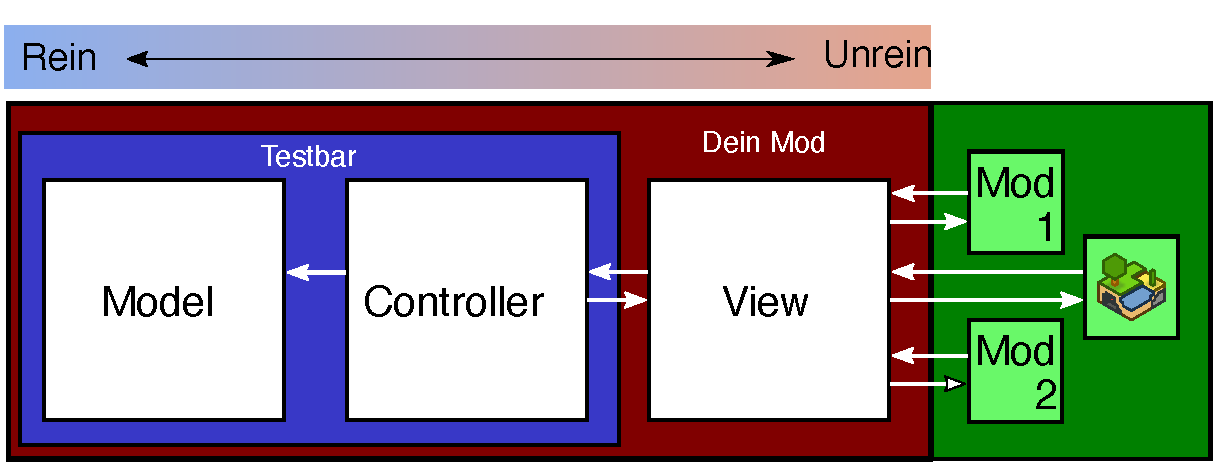
\includegraphics[width=12cm,height=\textheight,keepaspectratio,alt={Model, View und Controller und ihre Verbindungen}]{bilder/mvc_diagram.pdf}
\caption{Model, View und Controller und ihre Verbindungen}
\end{figure}

Wichtig ist, dass jeder Bereich nur mit seinen direkten Nachbarn
kommuniziert, wie im Diagramm gezeigt. So musst du weniger ändern, wenn
du das Innere oder die Schnittstelle eines Bereichs änderst. Um die
Formspec zu ändern, musst du zum Beispiel nur die View anpassen. Um die
API der View zu ändern, musst du nur View und Controller anpassen, das
Model aber gar nicht.

In der Praxis wird dieser Entwurf selten verwendet, weil er die
Komplexität erhöht und den meisten Mods nicht viel bringt. Häufiger
sieht man einen weniger formalen und strengen Entwurf -- Varianten von
API-View.

\subsection{API-View}\label{api-view}

In einer idealen Welt wären die drei Bereiche oben sauber getrennt, und
alle Ereignisse gingen erst durch den Controller, bevor sie zur View
zurückkehren. Die Welt ist aber nicht ideal. Ein guter Kompromiss ist,
den Mod in zwei Teile zu gliedern:

\begin{itemize}
\tightlist
\item
  \textbf{API} -- Das waren oben Model und Controller. Hier sollte
  \texttt{core.\allowbreak{}} nirgends vorkommen.
\item
  \textbf{View} -- Das war auch oben die View. Am besten teilst du sie
  in eigene Dateien für jede Art von Ereignis auf.
\end{itemize}

rubenwardys crafting-Mod\footnote{\url{https://github.com/rubenwardy/crafting}}
folgt ungefähr diesem Entwurf. \texttt{api.\allowbreak{}lua} besteht
fast nur aus reinen Lua-Funktionen für die Datenhaltung und Berechnungen
im Stil eines Controllers. \texttt{gui.\allowbreak{}lua} ist die View
für Formspecs und deren Eingaben, und
\texttt{async\_\allowbreak{}crafter.\allowbreak{}lua} ist View und
Controller für eine Node-Formspec und
Node-Timer.\index{node-timer@Node-Timer}

So aufgeteilt, lässt sich der API-Teil sehr einfach testen, weil er
keine Luanti-APIs verwendet -- wie im nächsten
Kapitel~(Kapitel~\ref{ch:quality/unit-testing}) gezeigt und im
crafting-Mod zu sehen.

\section{Fazit}\label{fazit}

Guter Code-Entwurf ist subjektiv und hängt stark vom jeweiligen Projekt
ab. Als Faustregel gilt: Halte die Kohäsion hoch und die Kopplung
gering. Anders gesagt: Halte zusammen, was zusammengehört, trenne, was
nicht zusammengehört, und halte die Abhängigkeiten einfach.

Sehr zu empfehlen ist das Buch Game Programming Patterns\footnote{\url{http://gameprogrammingpatterns.com/}}
(englisch). Es ist kostenlos online lesbar\footnote{\url{http://gameprogrammingpatterns.com/contents.html}}
und geht viel ausführlicher auf verbreitete Programmiermuster für Spiele
ein.

\chapter{Automatische Unit-Tests}
\label{ch:quality/unit-testing}

Unit-Tests\index{unit-test@Unit-Test} sind ein unverzichtbares Werkzeug,
um nachzuweisen und dich zu vergewissern, dass dein Code korrekt ist.
Dieses Kapitel zeigt, wie du mit \emph{Busted\index{busted@Busted}}
Tests für Luanti-Mods und -Spiele schreibst. Funktionen zu testen, die
Luanti-Funktionen aufrufen, ist ziemlich schwierig. Zum Glück haben wir
im vorigen Kapitel~(Kapitel~\ref{ch:quality/clean-arch}) besprochen, wie
du deinen Code so aufbaust, dass sich das vermeiden lässt.

\section{Busted installieren}\label{busted-installieren}

Zuerst installierst du LuaRocks:

\begin{itemize}
\tightlist
\item
  Windows: Folge der Installationsanleitung im LuaRocks-Wiki\footnote{\url{https://github.com/luarocks/luarocks/wiki/Installation-instructions-for-Windows}}
  (englisch).
\item
  Debian/Ubuntu: \texttt{sudo apt install luarocks}
\end{itemize}

Dann installierst du Busted global:

\begin{Shaded}
\begin{Highlighting}[]
\NormalTok{sudo luarocks install busted}
\end{Highlighting}
\end{Shaded}

Zum Schluss prüfst du, ob es installiert ist:

\begin{Shaded}
\begin{Highlighting}[]
\NormalTok{busted {-}{-}version}
\end{Highlighting}
\end{Shaded}

\section{Dein erster Test}\label{dein-erster-test}

Busted ist das führende Framework für Unit-Tests in Lua. Es sucht nach
Lua-Dateien, deren Name auf \texttt{\_\allowbreak{}spec} endet, und
führt sie in einer eigenständigen Lua-Umgebung aus.

\begin{Shaded}
\begin{Highlighting}[]
\NormalTok{mymod/}
\NormalTok{├── init.lua}
\NormalTok{├── api.lua}
\NormalTok{└── tests}
\NormalTok{    └── api\_spec.lua}
\end{Highlighting}
\end{Shaded}

\subsection{init.lua}\label{init.lua}

\begin{Shaded}
\begin{Highlighting}[]
\VariableTok{mymod} \OperatorTok{=} \OperatorTok{\{\}}

\FunctionTok{dofile}\OperatorTok{(}\VariableTok{core}\OperatorTok{.}\NormalTok{get\_modpath}\OperatorTok{(}\StringTok{"mymod"}\OperatorTok{)} \OperatorTok{..} \StringTok{"/api.lua"}\OperatorTok{)}
\end{Highlighting}
\end{Shaded}

\subsection{api.lua}\label{api.lua}

\begin{Shaded}
\begin{Highlighting}[]
\KeywordTok{function} \VariableTok{mymod}\OperatorTok{.}\NormalTok{add}\OperatorTok{(}\VariableTok{x}\OperatorTok{,} \VariableTok{y}\OperatorTok{)}
    \ControlFlowTok{return} \VariableTok{x} \OperatorTok{+} \VariableTok{y}
\KeywordTok{end}
\end{Highlighting}
\end{Shaded}

\subsection{tests/api\_spec.lua}\label{testsapi_spec.lua}

\begin{Shaded}
\begin{Highlighting}[]
\CommentTok{{-}{-} Benötigte Dateien im Mod{-}Verzeichnis suchen}
\VariableTok{package.path} \OperatorTok{=} \StringTok{"./?.lua;"} \OperatorTok{..} \VariableTok{package.path}

\CommentTok{{-}{-} Globale Tabelle mymod anlegen, in die die API schreibt}
\ConstantTok{\_G}\OperatorTok{.}\VariableTok{mymod} \OperatorTok{=} \OperatorTok{\{\}}
\CommentTok{{-}{-} api.lua ausführen}
\FunctionTok{require}\OperatorTok{(}\StringTok{"api"}\OperatorTok{)}

\CommentTok{{-}{-} Tests}
\NormalTok{describe}\OperatorTok{(}\StringTok{"add"}\OperatorTok{,} \KeywordTok{function}\OperatorTok{()}
\NormalTok{    it}\OperatorTok{(}\StringTok{"addiert"}\OperatorTok{,} \KeywordTok{function}\OperatorTok{()}
        \VariableTok{assert}\OperatorTok{.}\NormalTok{equals}\OperatorTok{(}\DecValTok{2}\OperatorTok{,} \VariableTok{mymod}\OperatorTok{.}\NormalTok{add}\OperatorTok{(}\DecValTok{1}\OperatorTok{,} \DecValTok{1}\OperatorTok{))}
    \KeywordTok{end}\OperatorTok{)}

\NormalTok{    it}\OperatorTok{(}\StringTok{"kann mit negativen Zahlen umgehen"}\OperatorTok{,} \KeywordTok{function}\OperatorTok{()}
        \VariableTok{assert}\OperatorTok{.}\NormalTok{equals}\OperatorTok{(}\DecValTok{0}\OperatorTok{,} \VariableTok{mymod}\OperatorTok{.}\NormalTok{add}\OperatorTok{({-}}\DecValTok{1}\OperatorTok{,} \DecValTok{1}\OperatorTok{))}
        \VariableTok{assert}\OperatorTok{.}\NormalTok{equals}\OperatorTok{({-}}\DecValTok{2}\OperatorTok{,} \VariableTok{mymod}\OperatorTok{.}\NormalTok{add}\OperatorTok{({-}}\DecValTok{1}\OperatorTok{,} \OperatorTok{{-}}\DecValTok{1}\OperatorTok{))}
    \KeywordTok{end}\OperatorTok{)}
\KeywordTok{end}\OperatorTok{)}
\end{Highlighting}
\end{Shaded}

Jetzt kannst du die Tests ausführen, indem du im Verzeichnis des Mods
ein Terminal öffnest und \texttt{busted .\allowbreak{}} aufrufst.

Wichtig ist, dass die API-Datei die Tabelle nicht selbst anlegt, denn
globale Variablen funktionieren in Busted anders. Jede Variable, die in
Luanti global wäre, ist in Busted lokal zur Datei. Das wäre auch für
Luanti der bessere Weg gewesen, aber dafür ist es jetzt zu spät.

Außerdem sollten die Dateien, die du testest, möglichst keine Funktionen
aufrufen, die nicht in ihnen selbst stehen. Meist schreibst du Tests
jeweils nur für eine einzelne Datei.

\section{Mocking: Externe Funktionen
ersetzen}\label{mocking-externe-funktionen-ersetzen}

\emph{Mocking\index{mocking@Mocking}} heißt, Funktionen zu ersetzen, von
denen das Getestete abhängt. Das hat zwei Zwecke: Zum einen steht die
Funktion in der Testumgebung womöglich nicht zur Verfügung, zum anderen
möchtest du vielleicht Aufrufe der Funktion und ihre Argumente
mitschneiden.

Hast du die Ratschläge aus dem Kapitel Saubere
Architektur~(Kapitel~\ref{ch:quality/clean-arch}) befolgt, hast du schon
eine recht saubere Datei zum Testen. Dinge außerhalb deines Bereichs
musst du aber trotzdem ersetzen -- etwa die View, wenn du Controller
oder API testest. Hast du die Ratschläge nicht befolgt, wird es etwas
schwieriger, weil du womöglich die Luanti-API ersetzen musst.

\begin{Shaded}
\begin{Highlighting}[]
\CommentTok{{-}{-} Wie oben eine Tabelle anlegen}
\ConstantTok{\_G}\OperatorTok{.}\VariableTok{core} \OperatorTok{=} \OperatorTok{\{\}}

\CommentTok{{-}{-} Die Mock{-}Funktion definieren}
\KeywordTok{local} \VariableTok{chat\_send\_player\_calls} \OperatorTok{=} \OperatorTok{\{\}}
\KeywordTok{function} \VariableTok{core}\OperatorTok{.}\NormalTok{chat\_send\_player}\OperatorTok{(}\VariableTok{name}\OperatorTok{,} \VariableTok{message}\OperatorTok{)}
    \FunctionTok{table.insert}\OperatorTok{(}
        \VariableTok{chat\_send\_player\_calls}\OperatorTok{,}
        \OperatorTok{\{} \VariableTok{name} \OperatorTok{=} \VariableTok{name}\OperatorTok{,} \VariableTok{message} \OperatorTok{=} \VariableTok{message} \OperatorTok{\}}
    \OperatorTok{)}
\KeywordTok{end}

\CommentTok{{-}{-} Tests}
\NormalTok{describe}\OperatorTok{(}\StringTok{"list\_areas"}\OperatorTok{,} \KeywordTok{function}\OperatorTok{()}
\NormalTok{    it}\OperatorTok{(}\StringTok{"gibt eine Zeile je Gebiet aus"}\OperatorTok{,} \KeywordTok{function}\OperatorTok{()}
        \VariableTok{chat\_send\_player\_calls} \OperatorTok{=} \OperatorTok{\{\}} \CommentTok{{-}{-} Tabelle zurücksetzen}

        \VariableTok{mymod}\OperatorTok{.}\NormalTok{list\_areas\_to\_chat}\OperatorTok{(}
            \StringTok{"singleplayer"}\OperatorTok{,}
            \StringTok{"singleplayer"}
        \OperatorTok{)}

        \VariableTok{assert}\OperatorTok{.}\NormalTok{equals}\OperatorTok{(}\DecValTok{2}\OperatorTok{,} \OperatorTok{\#}\VariableTok{chat\_send\_player\_calls}\OperatorTok{)}
    \KeywordTok{end}\OperatorTok{)}

\NormalTok{    it}\OperatorTok{(}\StringTok{"sendet an den richtigen Spieler"}\OperatorTok{,} \KeywordTok{function}\OperatorTok{()}
        \VariableTok{chat\_send\_player\_calls} \OperatorTok{=} \OperatorTok{\{\}} \CommentTok{{-}{-} Tabelle zurücksetzen}

        \VariableTok{mymod}\OperatorTok{.}\NormalTok{list\_areas\_to\_chat}\OperatorTok{(}
            \StringTok{"singleplayer"}\OperatorTok{,}
            \StringTok{"singleplayer"}
        \OperatorTok{)}

        \ControlFlowTok{for} \ConstantTok{\_}\OperatorTok{,} \VariableTok{call} \KeywordTok{in} \FunctionTok{pairs}\OperatorTok{(}\VariableTok{chat\_send\_player\_calls}\OperatorTok{)} \ControlFlowTok{do}
            \VariableTok{assert}\OperatorTok{.}\NormalTok{equals}\OperatorTok{(}\StringTok{"singleplayer"}\OperatorTok{,} \VariableTok{call}\OperatorTok{.}\VariableTok{name}\OperatorTok{)}
        \ControlFlowTok{end}
    \KeywordTok{end}\OperatorTok{)}

    \CommentTok{{-}{-} Die beiden Tests oben sind eigentlich überflüssig,}
    \CommentTok{{-}{-} denn dieser prüft beides}
\NormalTok{    it}\OperatorTok{(}\StringTok{"gibt das Richtige aus"}\OperatorTok{,} \KeywordTok{function}\OperatorTok{()}
        \VariableTok{chat\_send\_player\_calls} \OperatorTok{=} \OperatorTok{\{\}} \CommentTok{{-}{-} Tabelle zurücksetzen}

        \VariableTok{mymod}\OperatorTok{.}\NormalTok{list\_areas\_to\_chat}\OperatorTok{(}
            \StringTok{"singleplayer"}\OperatorTok{,}
            \StringTok{"singleplayer"}
        \OperatorTok{)}

        \KeywordTok{local} \VariableTok{expected} \OperatorTok{=} \OperatorTok{\{}
            \OperatorTok{\{}
                \VariableTok{name} \OperatorTok{=} \StringTok{"singleplayer"}\OperatorTok{,}
                \VariableTok{message} \OperatorTok{=} \StringTok{"Rathaus (2,43,63)"}\OperatorTok{,}
            \OperatorTok{\},}
            \OperatorTok{\{}
                \VariableTok{name} \OperatorTok{=} \StringTok{"singleplayer"}\OperatorTok{,}
                \VariableTok{message} \OperatorTok{=} \StringTok{"Flughafen (43,45,63)"}\OperatorTok{,}
            \OperatorTok{\},}
        \OperatorTok{\}}
        \VariableTok{assert}\OperatorTok{.}\NormalTok{same}\OperatorTok{(}\VariableTok{expected}\OperatorTok{,} \VariableTok{chat\_send\_player\_calls}\OperatorTok{)}
    \KeywordTok{end}\OperatorTok{)}
\KeywordTok{end}\OperatorTok{)}
\end{Highlighting}
\end{Shaded}

\section{Fazit}\label{fazit}

Gut eingesetzt, verbessern Unit-Tests die Qualität und Zuverlässigkeit
deines Projekts erheblich. Sie verlangen aber, dass du deinen Code
anders aufbaust als üblich.

Ein Beispiel für einen Mod mit vielen Unit-Tests ist crafting von
rubenwardy\footnote{\url{https://github.com/rubenwardy/crafting}}.

\chapter{Einen Mod veröffentlichen}
\label{ch:quality/releasing}

Wenn du einen Mod veröffentlichst, können andere ihn nutzen. Ein
veröffentlichter Mod wird womöglich in Einzelspielerwelten oder auf
Servern verwendet, auch auf öffentlichen.

\section{Eine Lizenz wählen}\label{eine-lizenz-wuxe4hlen}

Du musst für deinen Mod eine Lizenz\index{lizenz@Lizenz} angeben. Sie
sagt anderen, auf welche Weise sie dein Werk nutzen dürfen. Hat dein Mod
keine Lizenz, wissen andere nicht, ob sie ihn verändern, weitergeben
oder auf einem öffentlichen Server einsetzen dürfen.

Code und Grafiken stellen unterschiedliche Anforderungen an ihre
Lizenzen. Creative-Commons-Lizenzen solltest du zum Beispiel nicht für
Quellcode verwenden; für künstlerische Werke wie Bilder, Texte und
Meshes\index{mesh@Mesh} können sie aber gut geeignet sein.

Du darfst jede Lizenz verwenden. Mods, die keine Bearbeitungen erlauben,
sind im offiziellen Luanti-Forum allerdings nicht zugelassen. (Damit ein
Mod im Forum erlaubt ist, müssen andere Entwickler ihn verändern und die
veränderte Fassung veröffentlichen dürfen.)

Beachte, dass \textbf{Gemeinfreiheit (\emph{public domain}) keine
gültige Lizenz ist}, weil sie in verschiedenen Ländern unterschiedlich
definiert ist.

Von der WTFPL wird dringend abgeraten\footnote{\url{https://content.luanti.org/help/wtfpl/}}
(englisch); manche verzichten auf deinen Mod, wenn er unter dieser
Lizenz steht.

\subsection{LGPL und CC BY-SA}\label{lgpl-und-cc-by-sa}

Diese Kombination ist in der Luanti-Community verbreitet; auch Luanti
und Minetest Game verwenden sie.

Du stellst deinen Code unter die LGPL 2.1 und deine Grafiken unter CC
BY-SA.

Das bedeutet:

\begin{itemize}
\tightlist
\item
  Jeder darf veränderte und unveränderte Fassungen bearbeiten,
  weitergeben und verkaufen.
\item
  Wer deinen Mod verändert, muss seine Fassung unter dieselbe Lizenz
  stellen.
\item
  Dein Urheberrechtsvermerk muss erhalten bleiben.
\end{itemize}

\subsection{CC0}\label{cc0}

Diese Lizenz eignet sich für Code und Grafiken und erlaubt jedem, mit
deinem Werk zu tun, was er will. Andere dürfen es also verändern,
weitergeben, verkaufen und auch ohne Namensnennung verwenden.

\subsection{MIT}\label{mit}

Eine verbreitete Lizenz für Code. Die einzige Bedingung für Nutzer
deines Codes ist, dass sie in allen Kopien des Codes oder wesentlicher
Teile davon denselben Urheberrechtsvermerk und dieselbe Lizenz beifügen.

\section{Verpacken}\label{verpacken}

Einige Dateien solltest du deinem Mod oder Spiel vor der
Veröffentlichung beilegen.

\subsection{README.txt}\label{readme.txt}

Die README sollte angeben:

\begin{itemize}
\tightlist
\item
  was der Mod oder das Spiel tut und wie man ihn benutzt,
\item
  unter welcher Lizenz er steht,
\item
  optional:

  \begin{itemize}
  \tightlist
  \item
    wo man Probleme melden oder Hilfe bekommen kann,
  \item
    Danksagungen.
  \end{itemize}
\end{itemize}

\subsection{mod.conf / game.conf}\label{mod.conf-game.conf}

Füge unbedingt einen Schlüssel \texttt{description} hinzu, der erklärt,
was dein Mod oder Spiel tut. Fasse dich kurz, ohne vage zu werden. Die
Beschreibung sollte kurz sein, weil sie im Inhaltsinstaller angezeigt
wird, wo wenig Platz ist.

Gutes Beispiel:

\begin{Shaded}
\begin{Highlighting}[]
\NormalTok{description = Fügt Suppen, Kuchen, Gebäck und Säfte hinzu.}
\end{Highlighting}
\end{Shaded}

Vermeide so etwas:

\begin{Shaded}
\begin{Highlighting}[]
\NormalTok{description = Der Essens{-}Mod für Luanti.}
\end{Highlighting}
\end{Shaded}

Das ist zu vage.

\subsection{screenshot.png}\label{screenshot.png}

Screenshots sollten das Seitenverhältnis 3:2 haben (3 Pixel Breite auf 2
Pixel Höhe) und mindestens 300 × 200 Pixel groß sein.

Der Screenshot wird in Luanti als Vorschaubild für den Inhalt angezeigt.

\section{Hochladen}\label{hochladen}

Damit Interessierte deinen Mod herunterladen können, musst du ihn an
einem öffentlich zugänglichen Ort hochladen. Dafür gibt es mehrere Wege.
Nimm den, der für dich am besten passt, solange er diese Anforderungen
erfüllt (und alle weiteren, die Forenmoderatoren vielleicht noch
hinzufügen):

\begin{itemize}
\tightlist
\item
  \textbf{Beständig} -- Die Website sollte nicht ohne Vorwarnung
  abgeschaltet werden.
\item
  \textbf{Direkter Link} -- Ein Klick auf einen Link sollte die Datei
  herunterladen, ohne dass man erst eine andere Seite ansehen muss.
\item
  \textbf{Virenfrei} -- Unseriöse Upload-Dienste enthalten womöglich
  unsichere Werbung.
\end{itemize}

Bei ContentDB\index{contentdb@ContentDB} kannst du ZIP-Dateien
hochladen; ContentDB erfüllt diese Anforderungen.

\subsection{Versionsverwaltung}\label{versionsverwaltung}

Ein Versionsverwaltungssystem (\emph{Version Control System}, VCS)
verwaltet Änderungen an Software und macht es oft leichter, sie zu
verbreiten und Beiträge anderer anzunehmen.

Die meisten Luanti-Modder verwenden Git und eine Plattform wie GitHub,
um ihren Code zu verbreiten.

Git kann anfangs schwierig sein. Hilfe findest du hier:

\begin{itemize}
\tightlist
\item
  Pro Git\footnote{\url{https://git-scm.com/book/de/v2}} -- kostenlos
  online lesbar, auch auf Deutsch.
\end{itemize}

\section{Auf ContentDB
veröffentlichen}\label{auf-contentdb-veruxf6ffentlichen}

ContentDB ist der offizielle Ort, um Inhalte wie Mods, Spiele und
Texturpakete zu finden und zu verbreiten. Benutzer finden Inhalte über
die Website oder laden und installieren sie direkt über das Hauptmenü
von Luanti.

Registriere dich bei ContentDB\footnote{\url{https://content.luanti.org}}
und füge deinen Inhalt hinzu. Lies unbedingt die Hinweise im
Hilfebereich.

\section{Forenthema}\label{forenthema}

Du kannst auch ein Forenthema anlegen, in dem Benutzer über dein Werk
sprechen können.

Themen für Mods gehören ins Forum „WIP Mods``\footnote{\url{https://forum.luanti.org/viewforum.php?f=9}}
(\emph{Work in Progress}), Themen für Spiele ins Forum „WIP
Games``\footnote{\url{https://forum.luanti.org/viewforum.php?f=50}}.
Wenn dein Mod für dich nicht mehr in Arbeit ist, kannst du beantragen,
dass das Thema verschoben wird\footnote{\url{https://forum.luanti.org/viewtopic.php?f=11&t=10418}},
und zwar nach „Mod Releases``.

Das Forenthema sollte ähnliche Inhalte wie die README haben, aber
werbender formuliert sein und einen Link zum Herunterladen enthalten.
Wenn möglich, zeig Screenshots deines Mods in Aktion.

Der Titel des Themas muss eines dieser Formate haben:

\begin{itemize}
\tightlist
\item
  {[}Mod{]} Titel des Mods {[}modname{]}
\item
  {[}Mod{]} Titel des Mods {[}Versionsnummer{]} {[}modname{]}
\end{itemize}

Zum Beispiel:

\begin{itemize}
\tightlist
\item
  {[}Mod{]} More Blox {[}0.1{]} {[}moreblox{]}
\end{itemize}

\chapter{Weiterlesen}
\label{ch:quality/readmore}

Wenn du dieses Buch durchgelesen hast, lohnt sich ein Blick auf die
folgenden Quellen.

\section{Modding für Luanti}\label{modding-fuxfcr-luanti}

\begin{itemize}
\tightlist
\item
  Die Lua-API-Referenz von Luanti: mehrseitige Fassung\footnote{\url{https://api.luanti.org/}}
  und einseitige Fassung\footnote{\url{https://github.com/luanti-org/luanti/blob/master/doc/lua_api.md}}
  (englisch).
\item
  Schau dir bestehende Mods\footnote{\url{https://forum.luanti.org/viewforum.php?f=11}}
  an.
\end{itemize}

\section{Programmieren in Lua}\label{programmieren-in-lua}

\begin{itemize}
\tightlist
\item
  Programming in Lua (PIL)\footnote{\url{http://www.lua.org/pil/}}
  (englisch).
\end{itemize}

\section{3D-Modellierung}\label{d-modellierung}

\begin{itemize}
\tightlist
\item
  Blender 3D: Noob to Pro\footnote{\url{https://en.wikibooks.org/wiki/Blender_3D:_Noob_to_Pro}}
  (englisch).
\item
  Blender mit Luanti verwenden\footnote{\url{https://docs.luanti.org/Using_Blender/}}
  (englisch).
\end{itemize}


% ---------------------------------------------------------------- Anhang
\backmatter
\printindex

\end{document}
